    \subsection{Общая физика: квантовая физика}
        
        \subsubsection{Аннотация}

            Курс <<Общая физика: квантовая физика>> получил смешанные отзывы.

            Лекции Кобякина А.С. получили в основном негативные отзывы. На основании развернутных отзывов респондентов Совет студентов и аспирантов ФРКТ просит заменить лектора.

            Преподаватели семинаров и лабораторных работ Аникин Ю.А., Виноградов С.В., Кубышкин А.В., Стожков В.Ю., Зубович Н.Ю., Хан Ф.В., Юрьев Ю.В. получили крайне положительные оценки от респондентов. Совет студентов и аспирантов ФРКТ предлагает поощрить перечисленных преподавателей.

            Совет студентов и аспирантов ФРКТ также просит донести развернутые отзывы до преподавателей.

            Руководствуясь результатами опроса, Совет студентов и аспирантов ФРКТ выдвигает следующие идеи по улучшению данного курса:
	        \begin{enumerate}
                \item заменить лектора Кобякина А.С. на более компетентного преподавателя, такого как Овчинкин В.А. или Глазков В.Н., чьи записи лекций уже пользуются популярностью среди студентов;
                \item уменьшить количество материала (или адаптировать курс), т.к. многие респонденты отметили сложность в освоении последних тем курса.
            \end{enumerate}

        \subsubsection{Общий отзыв студентов о курсе}

            \begin{figure}[H]
                \centering
                \begin{subfigure}[b]{0.45\textwidth}
                    \centering
                    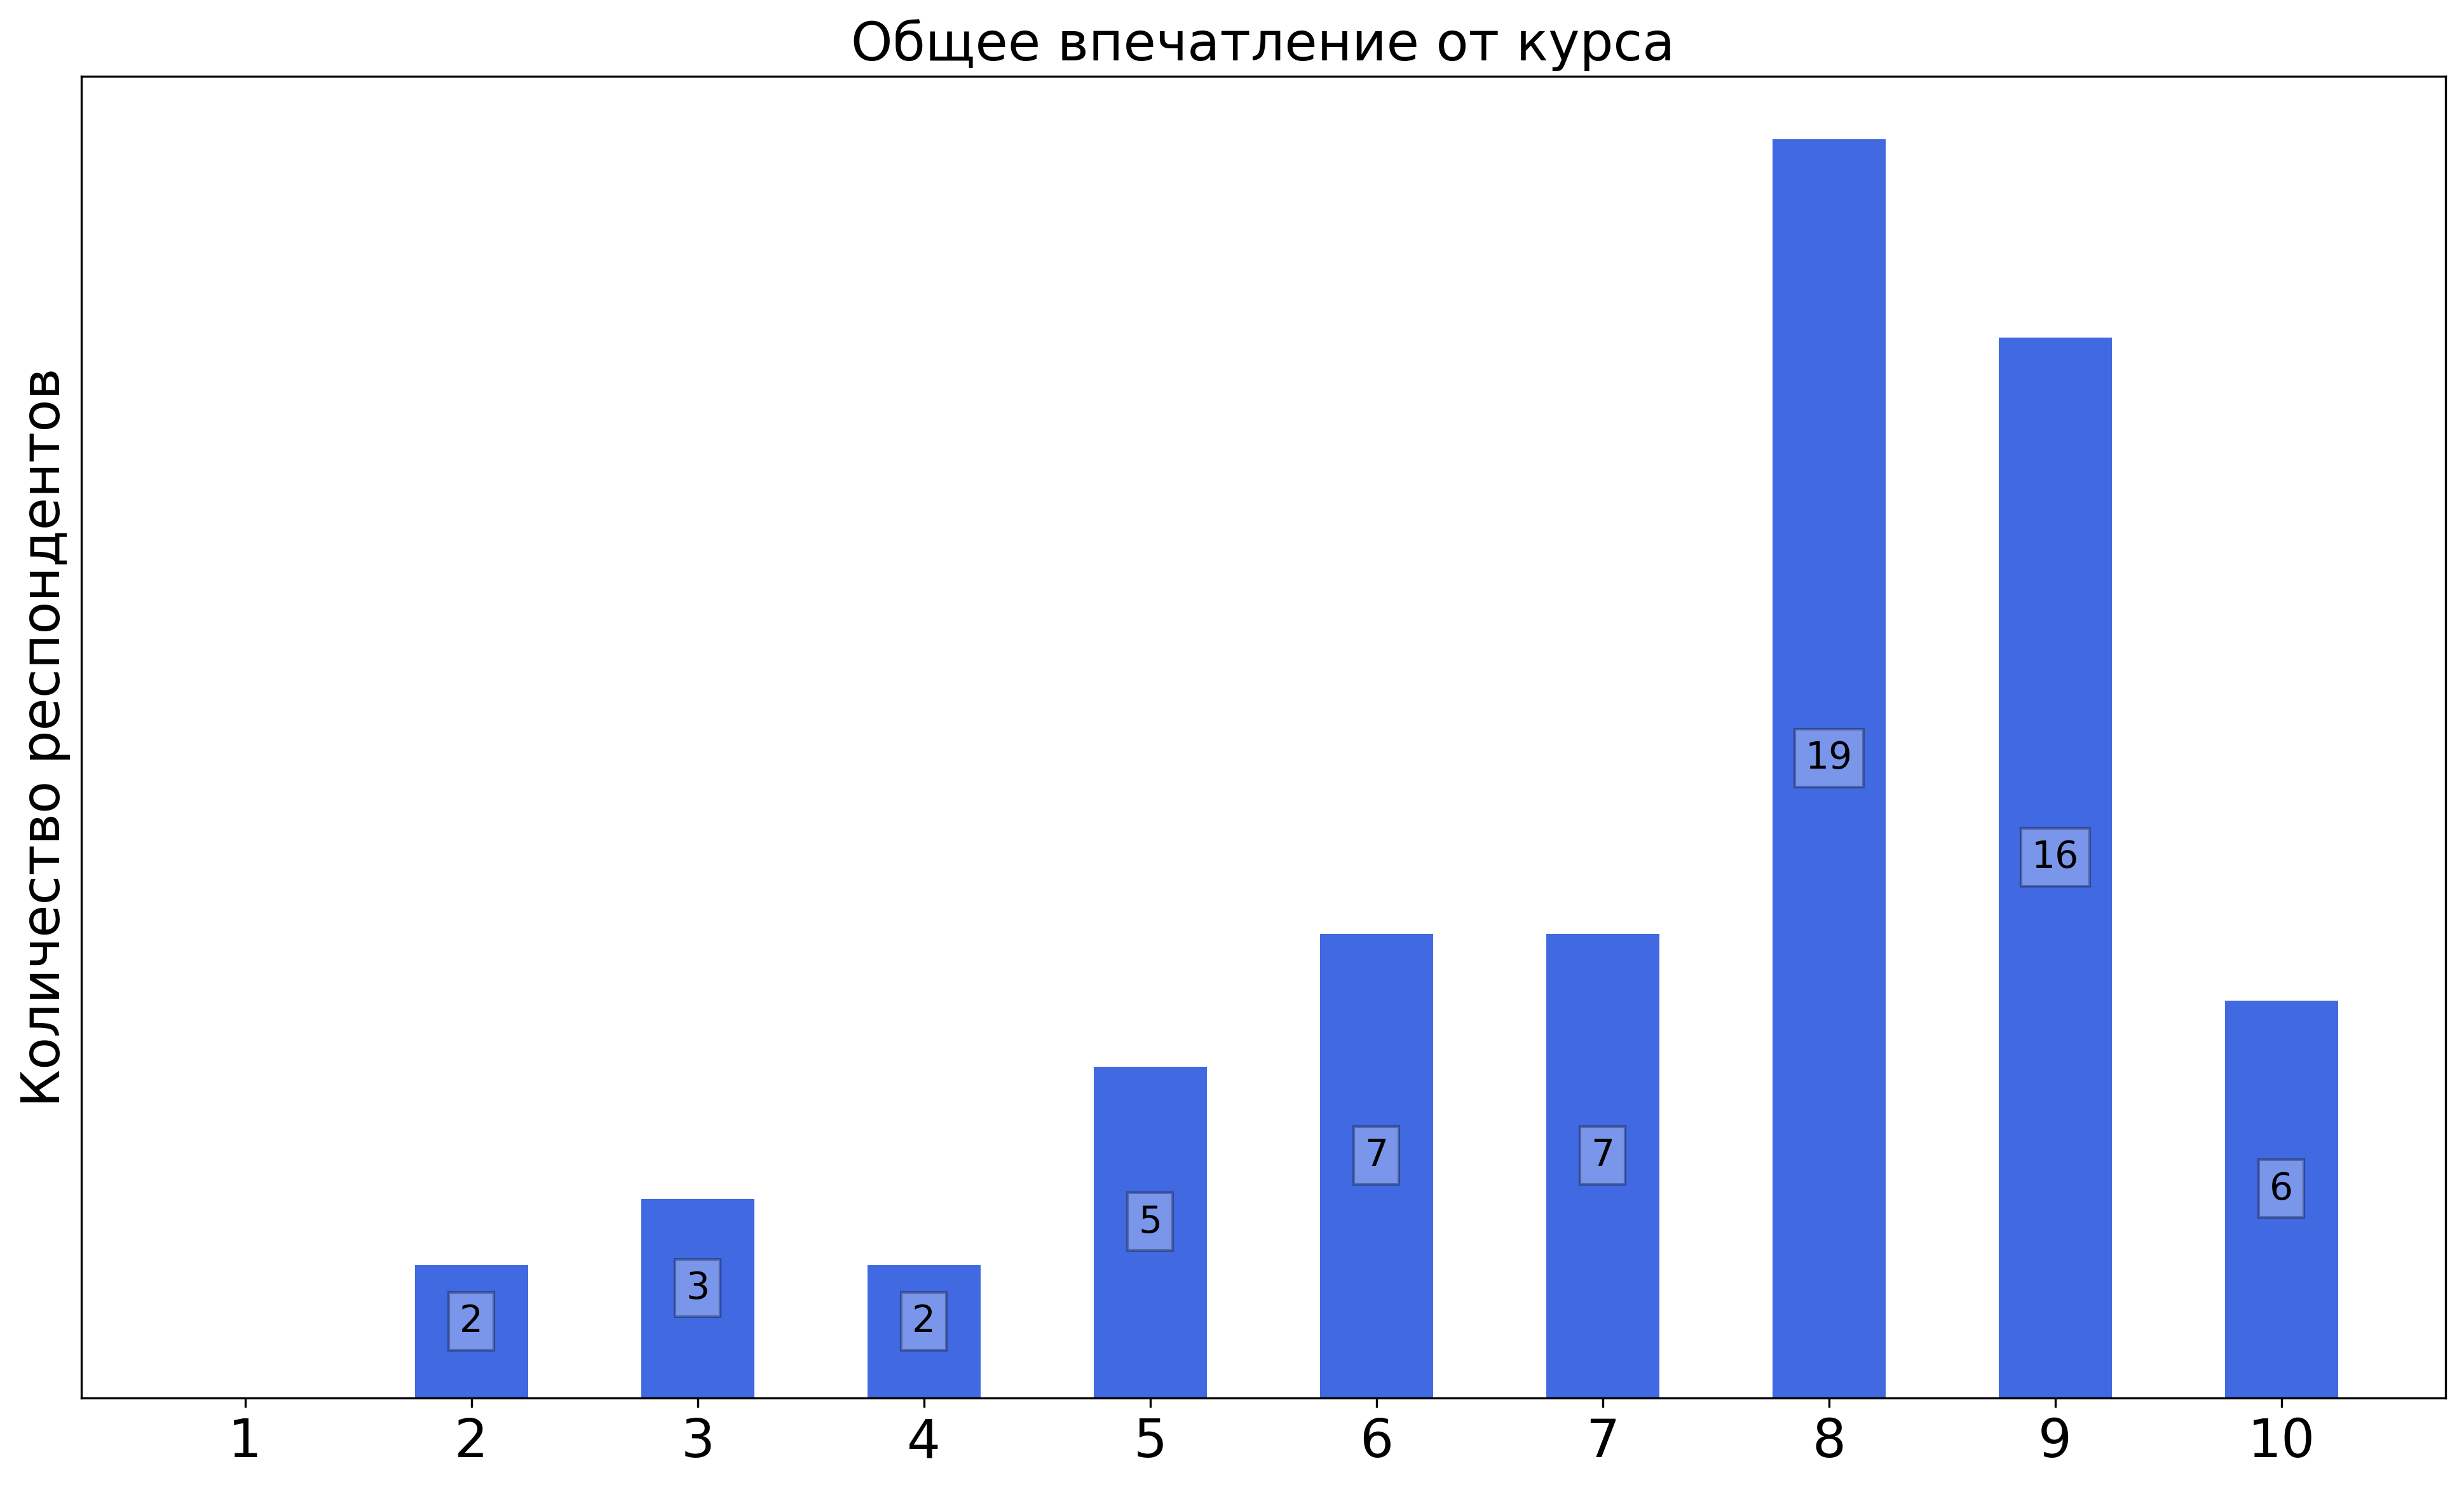
\includegraphics[width=\textwidth]{images/3 course/Общая физика - квантовая физика/general-0.png}
                \end{subfigure}
                \begin{subfigure}[b]{0.45\textwidth}
                    \centering
                    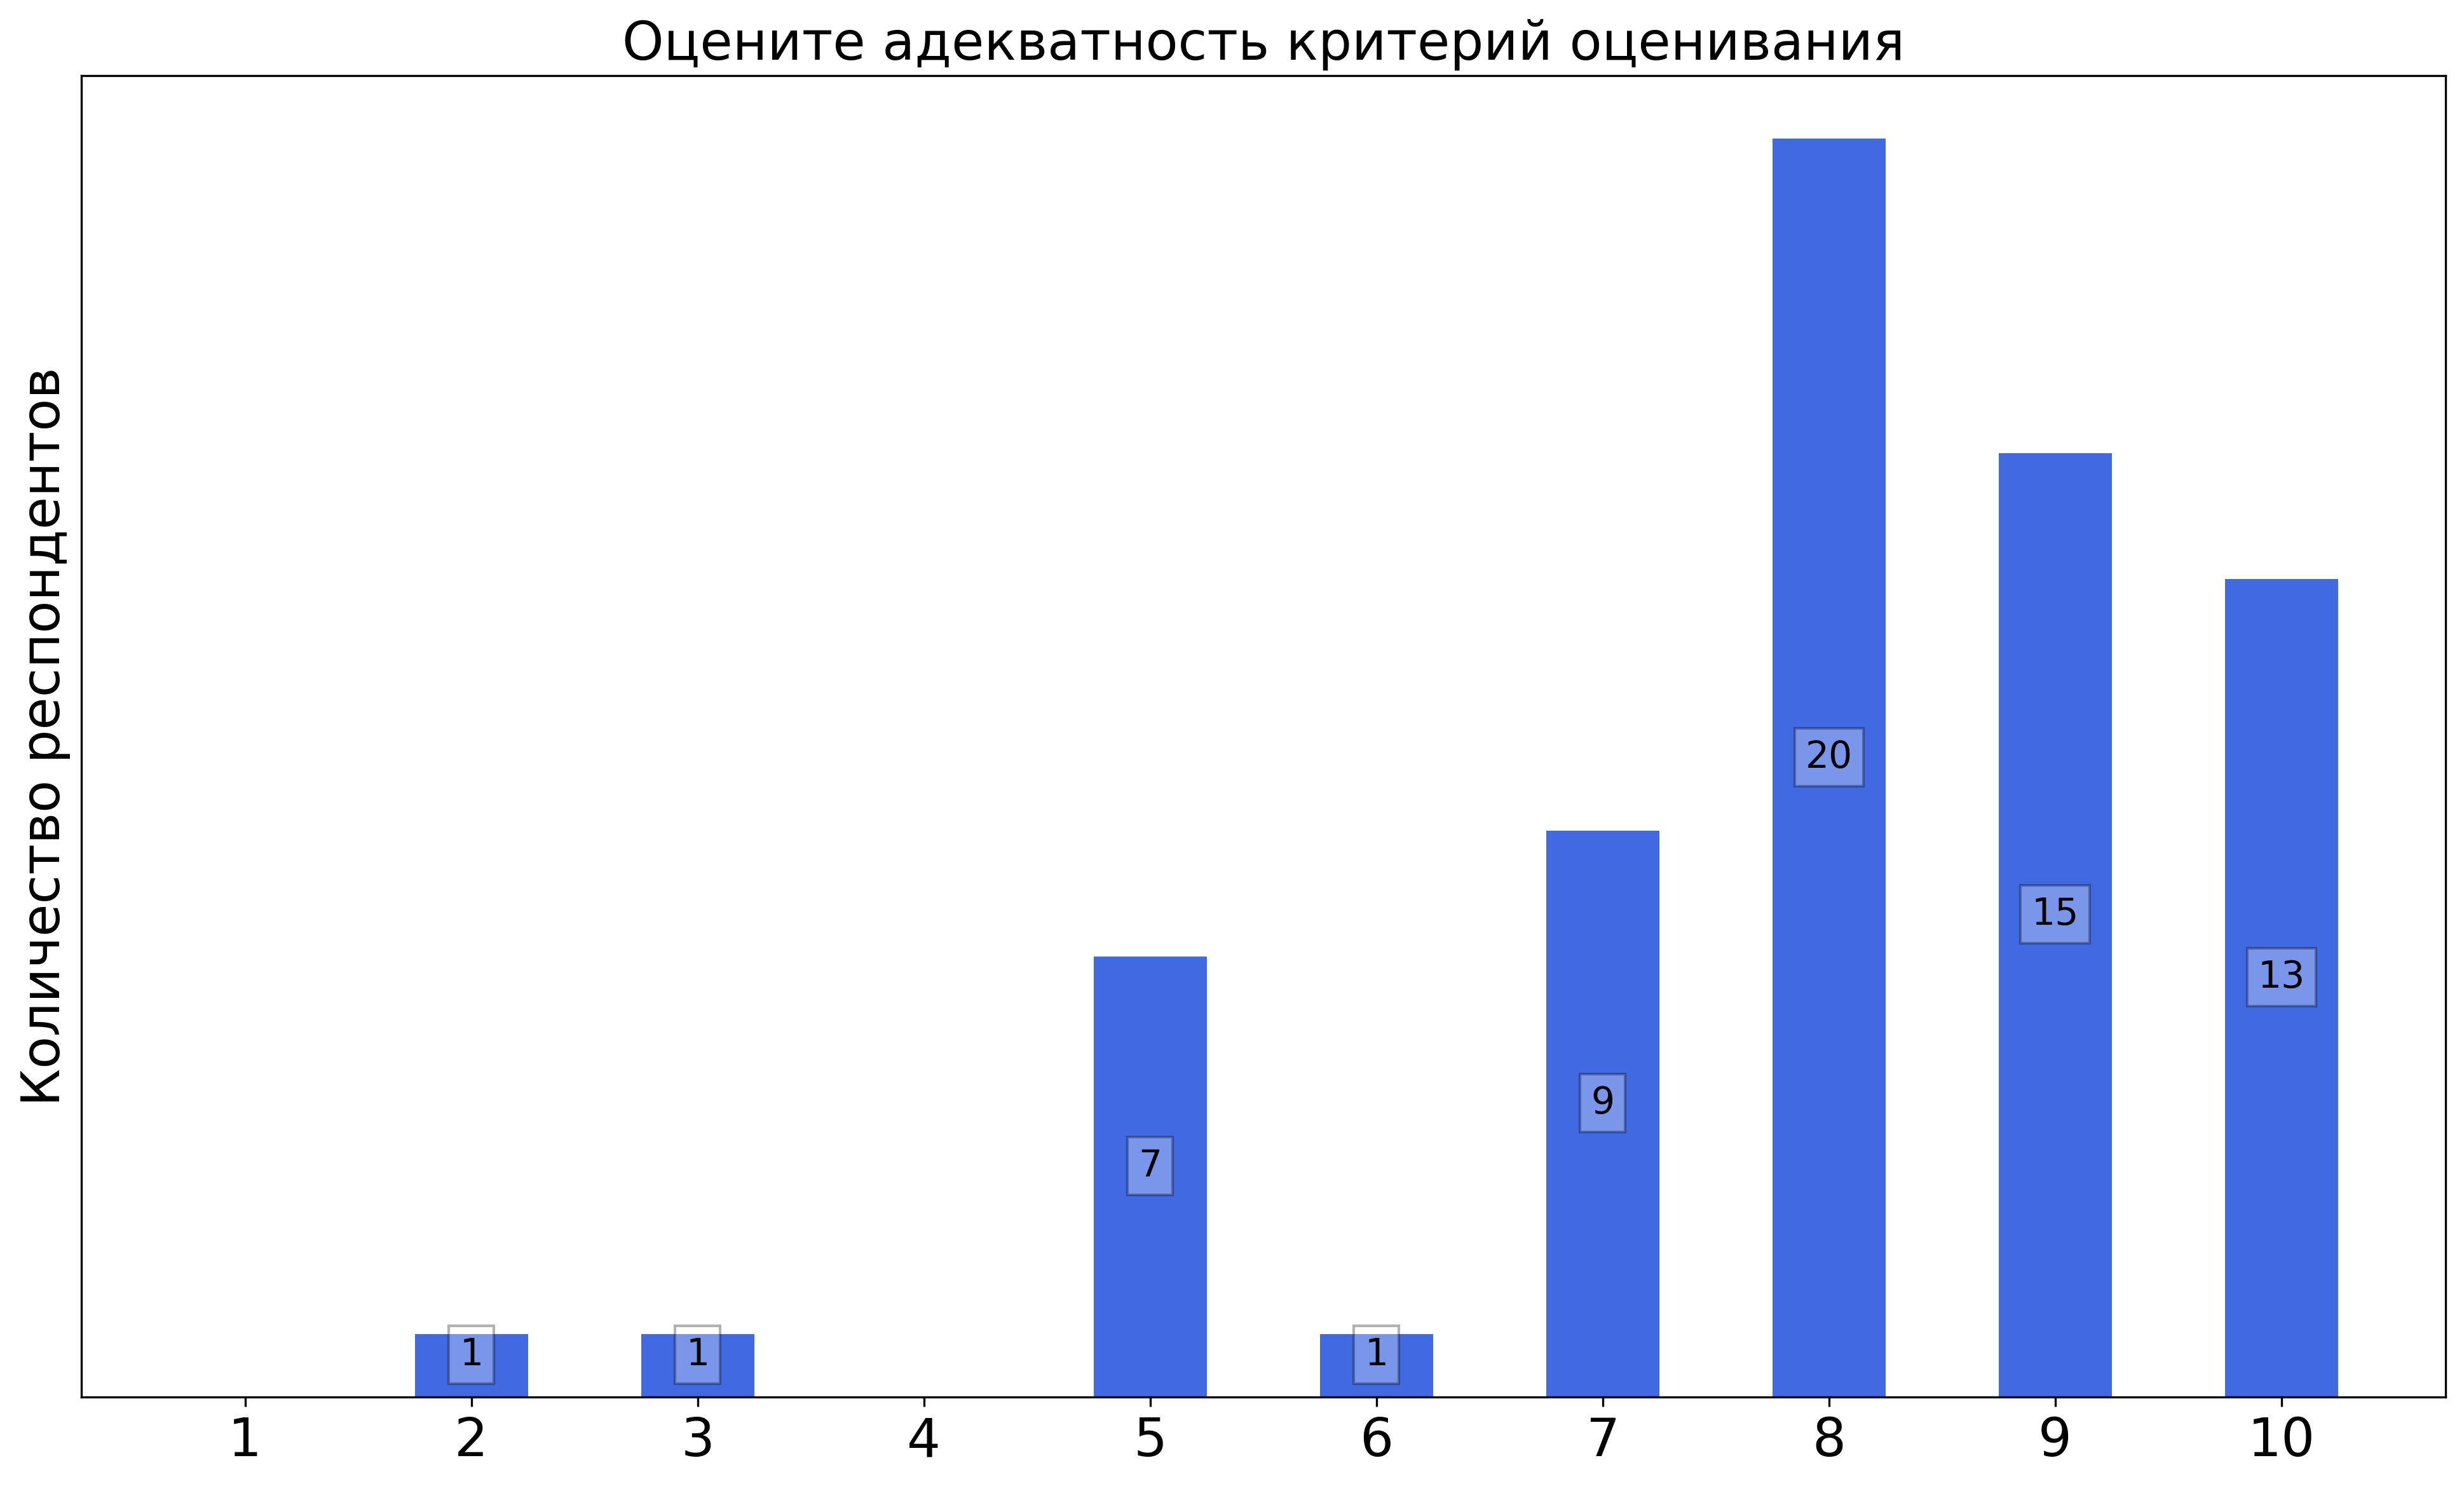
\includegraphics[width=\textwidth]{images/3 course/Общая физика - квантовая физика/general-1.png}
                \end{subfigure}	
            \end{figure}

        \subsubsection{Материалы, использумые респондентами при изучении курса}

            \begin{figure}[H]
                \centering
                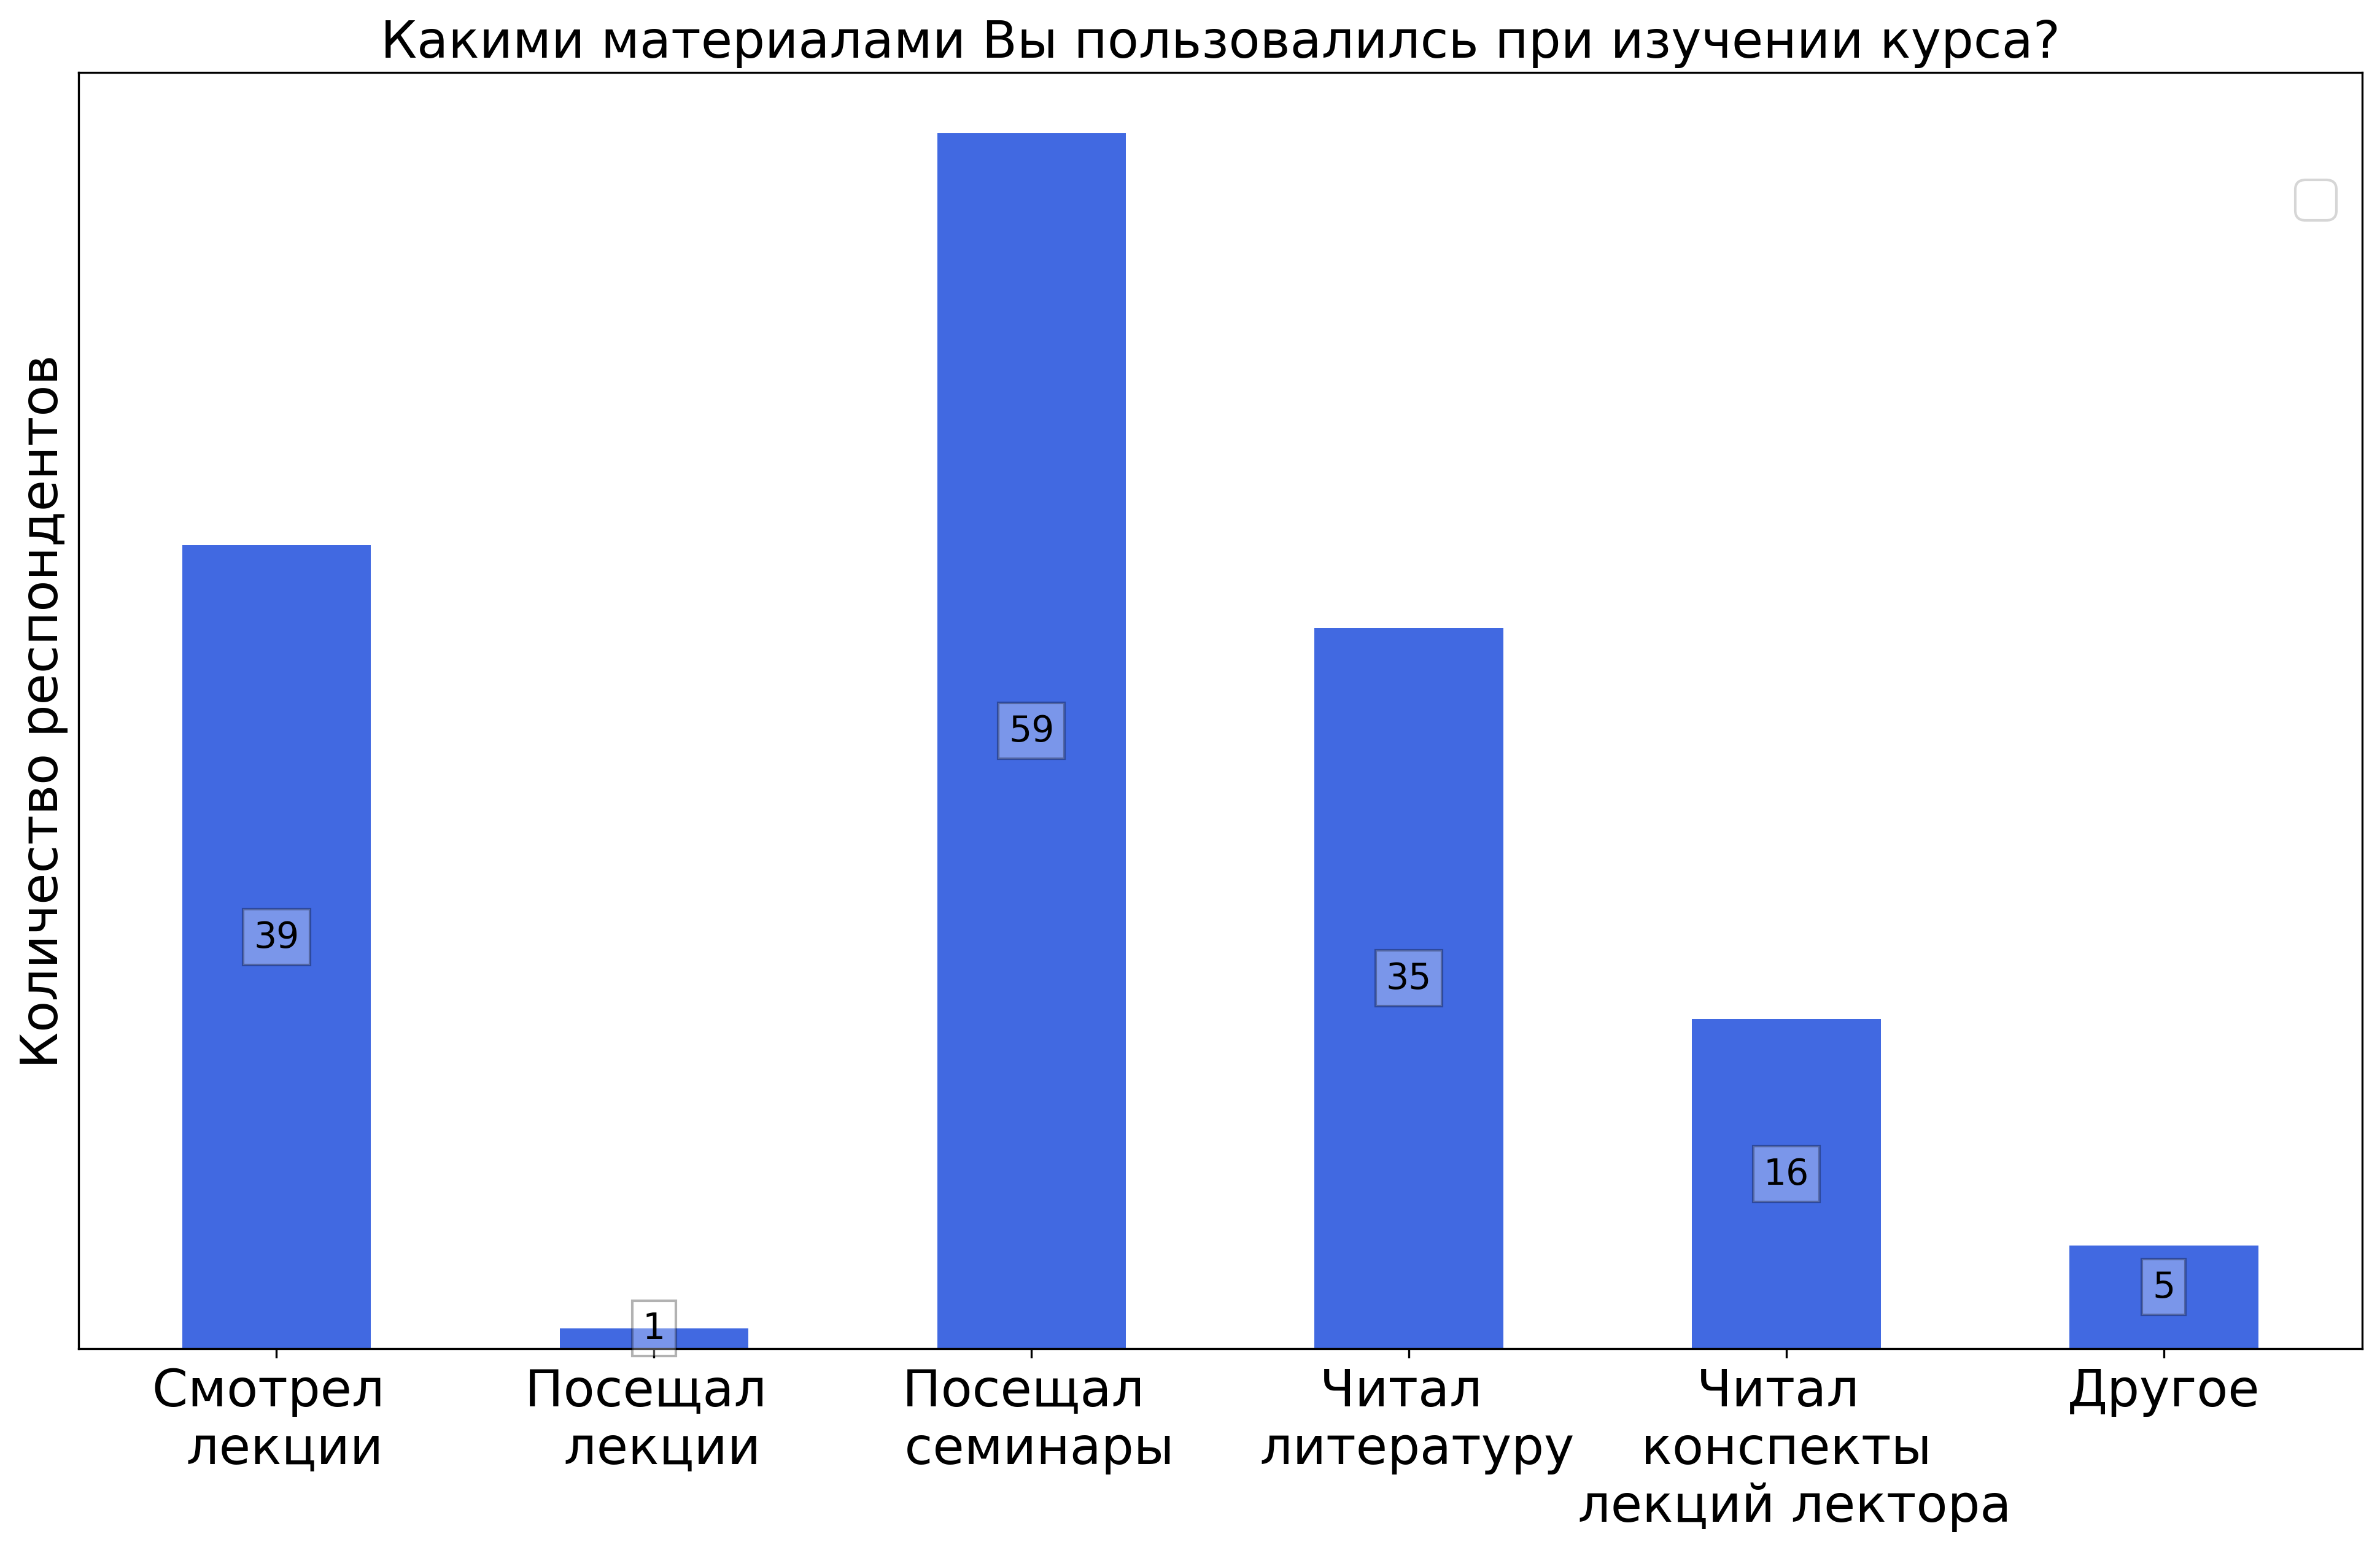
\includegraphics[width = 0.45\textwidth]{images/3 course/Общая физика - квантовая физика/materials.png}
            \end{figure}

            \textit{В качестве других источников информации студенты указали:} 
            \begin{itemize}
                \item онлайн-консультации Глазкова В.Н.;
                \item конспекты лекций прошлых лет;
                \item доп. семинары Овчинкина В.А.
            \end{itemize}

        \subsubsection{Отзыв студентов о лекциях. Лектор: Кобякин А.С.}

            \begin{figure}[H]
                \centering
                \begin{subfigure}[b]{0.45\textwidth}
                    \centering
                    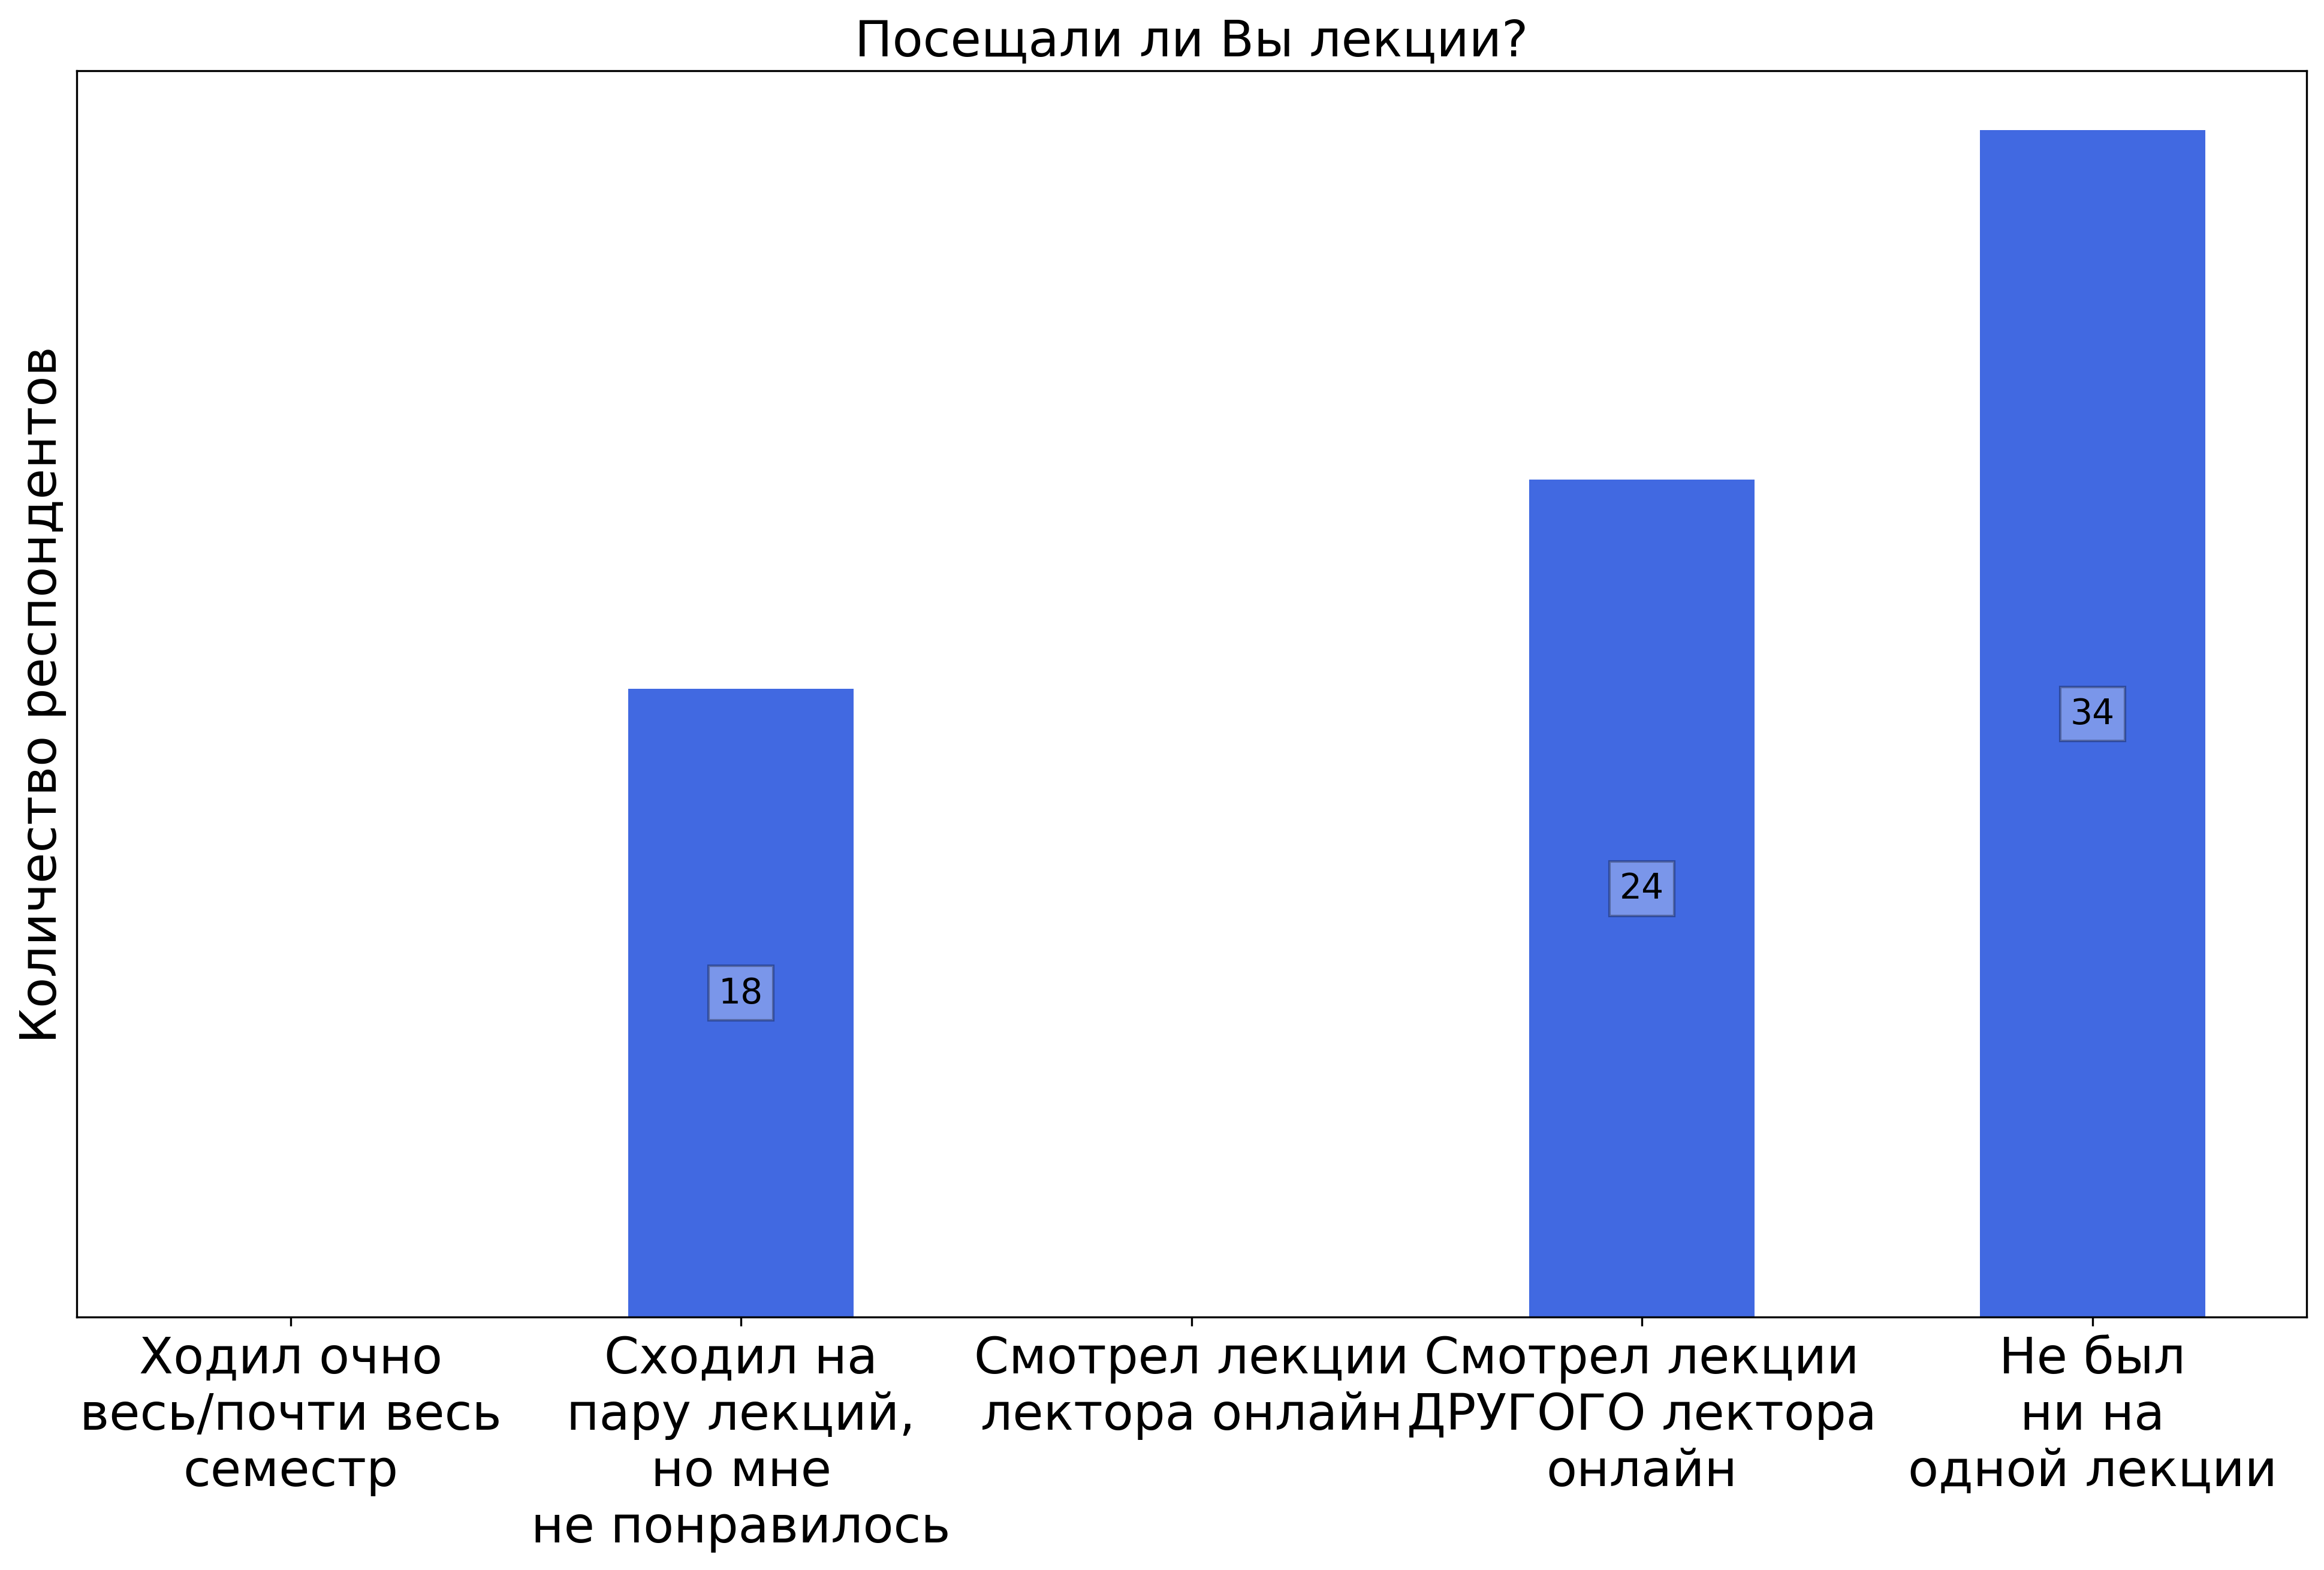
\includegraphics[width=\textwidth]{images/3 course/Общая физика - квантовая физика/lecturer-questions-Кобякин А.С.-0.png}
                \end{subfigure}
                \begin{subfigure}[b]{0.45\textwidth}
                    \centering
                    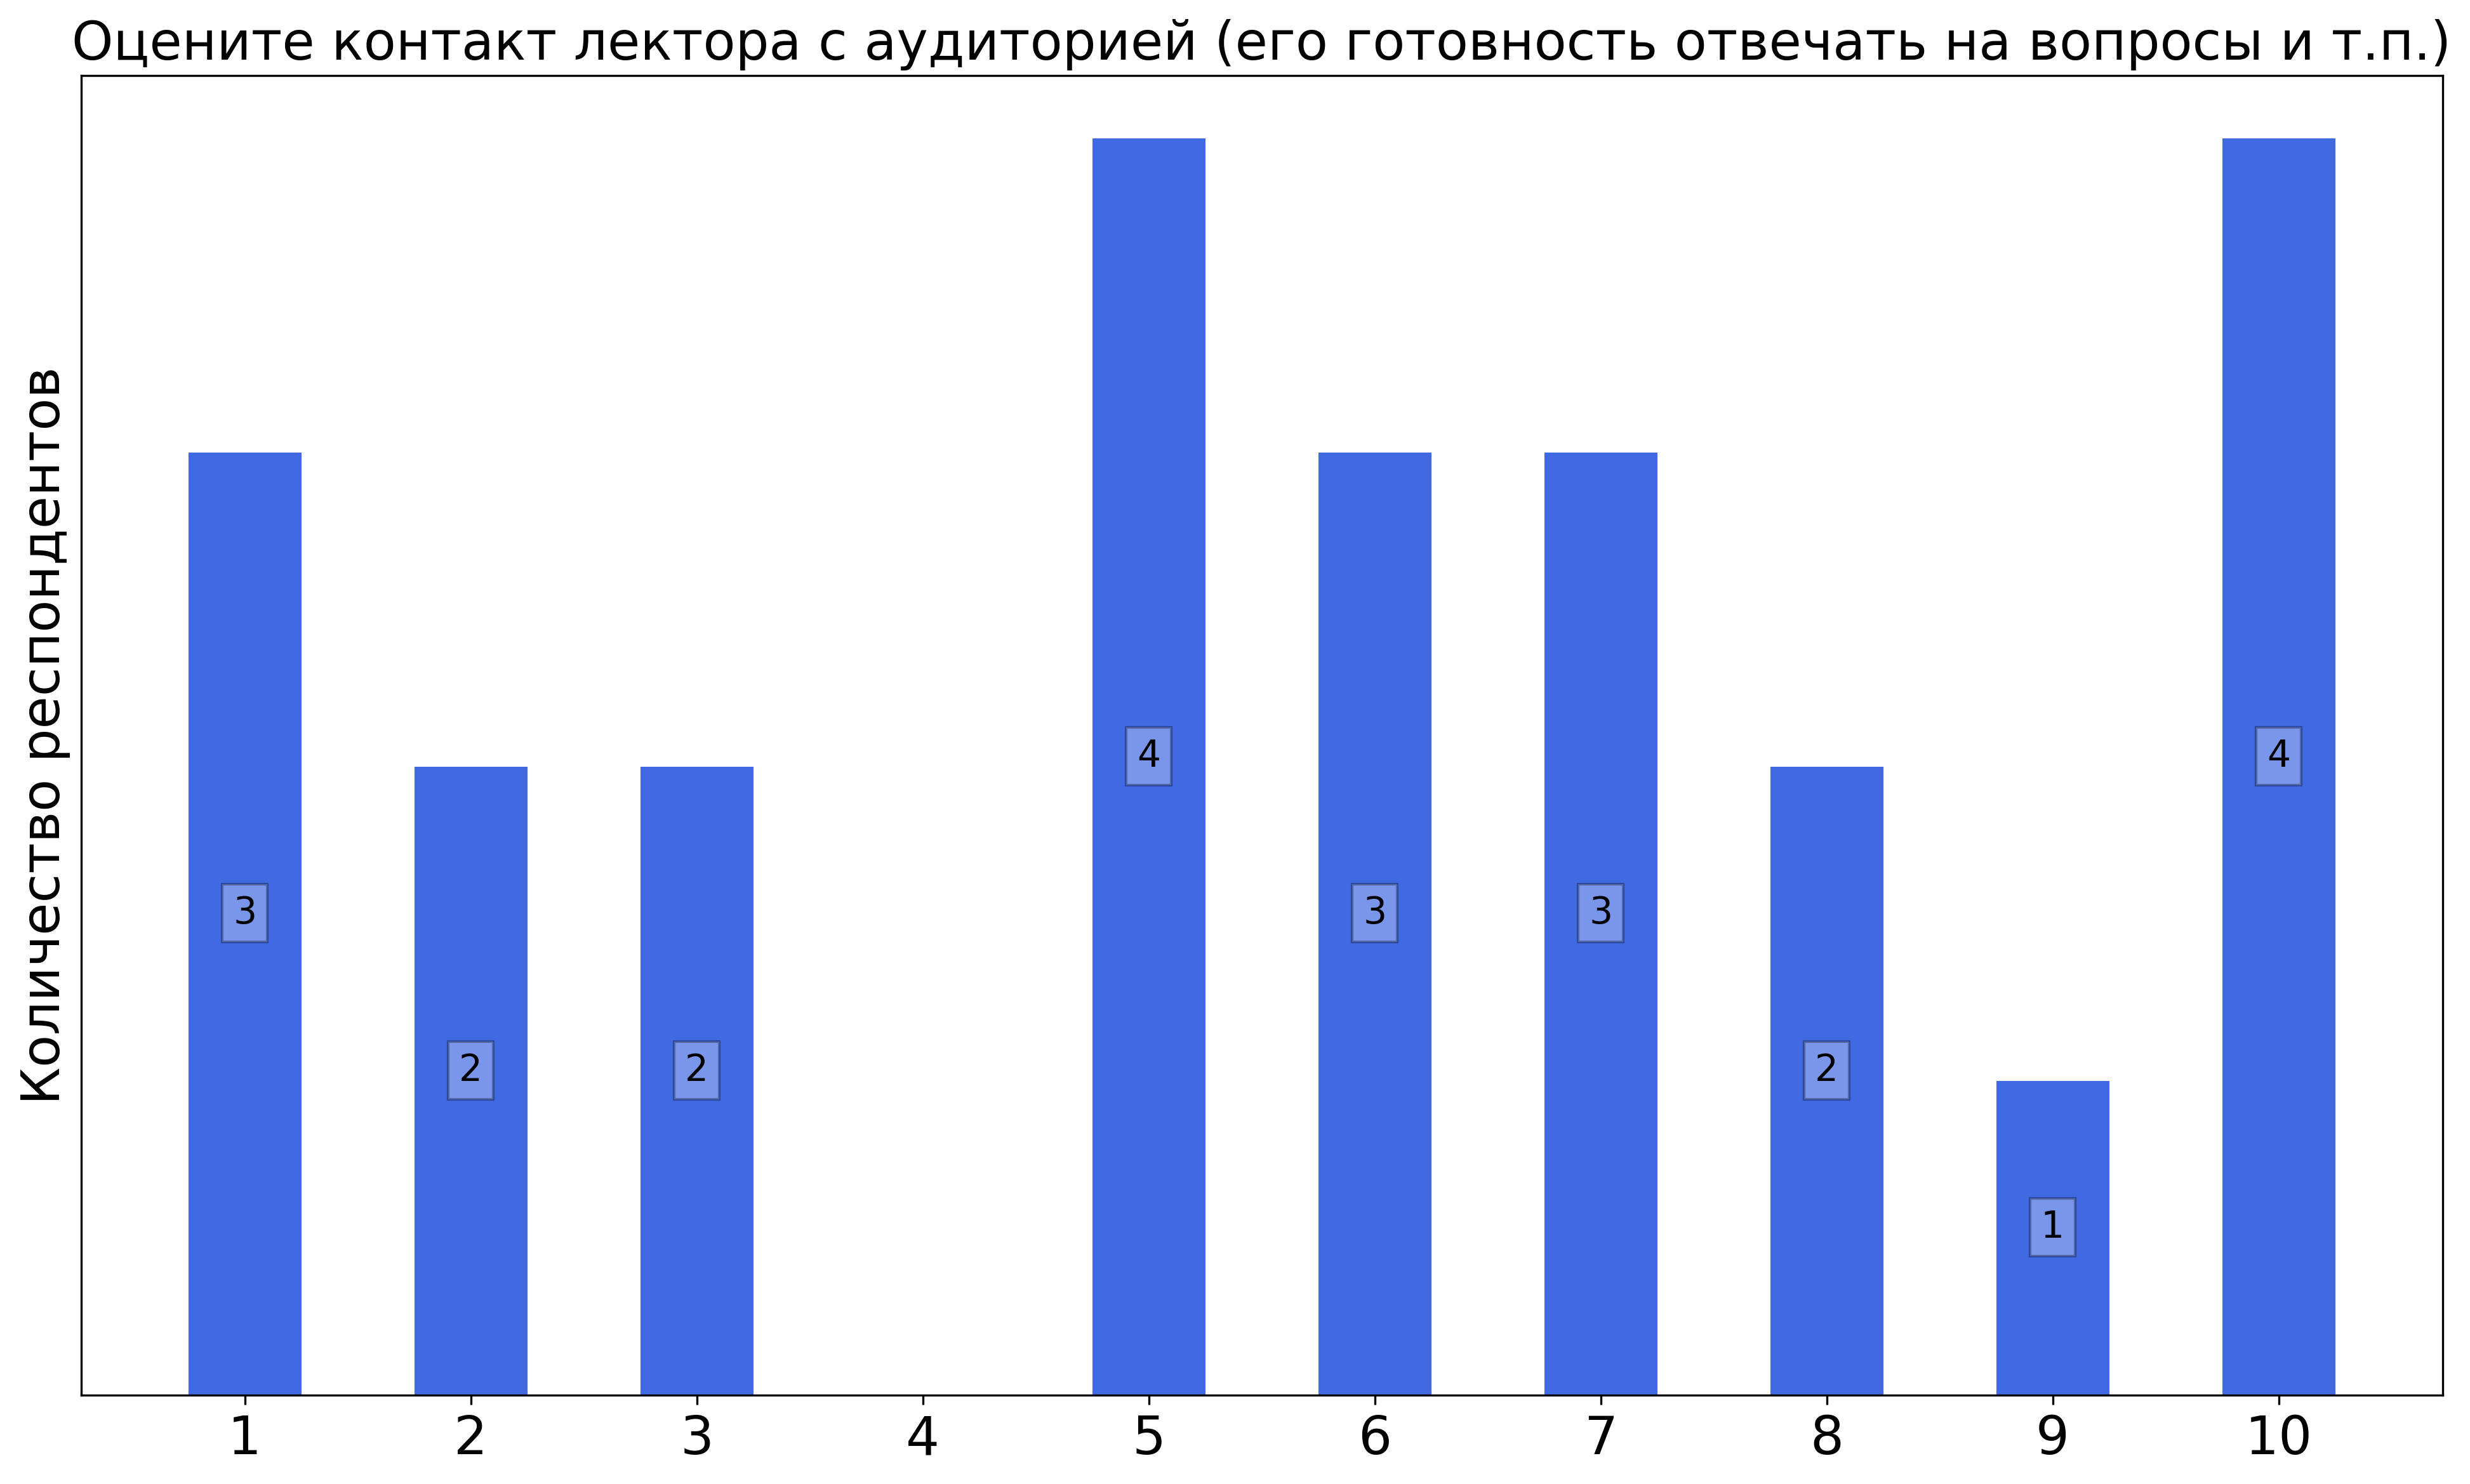
\includegraphics[width=\textwidth]{images/3 course/Общая физика - квантовая физика/lecturer-marks-Кобякин А.С.-0.png}
                \end{subfigure}
                \begin{subfigure}[b]{0.45\textwidth}
                    \centering
                    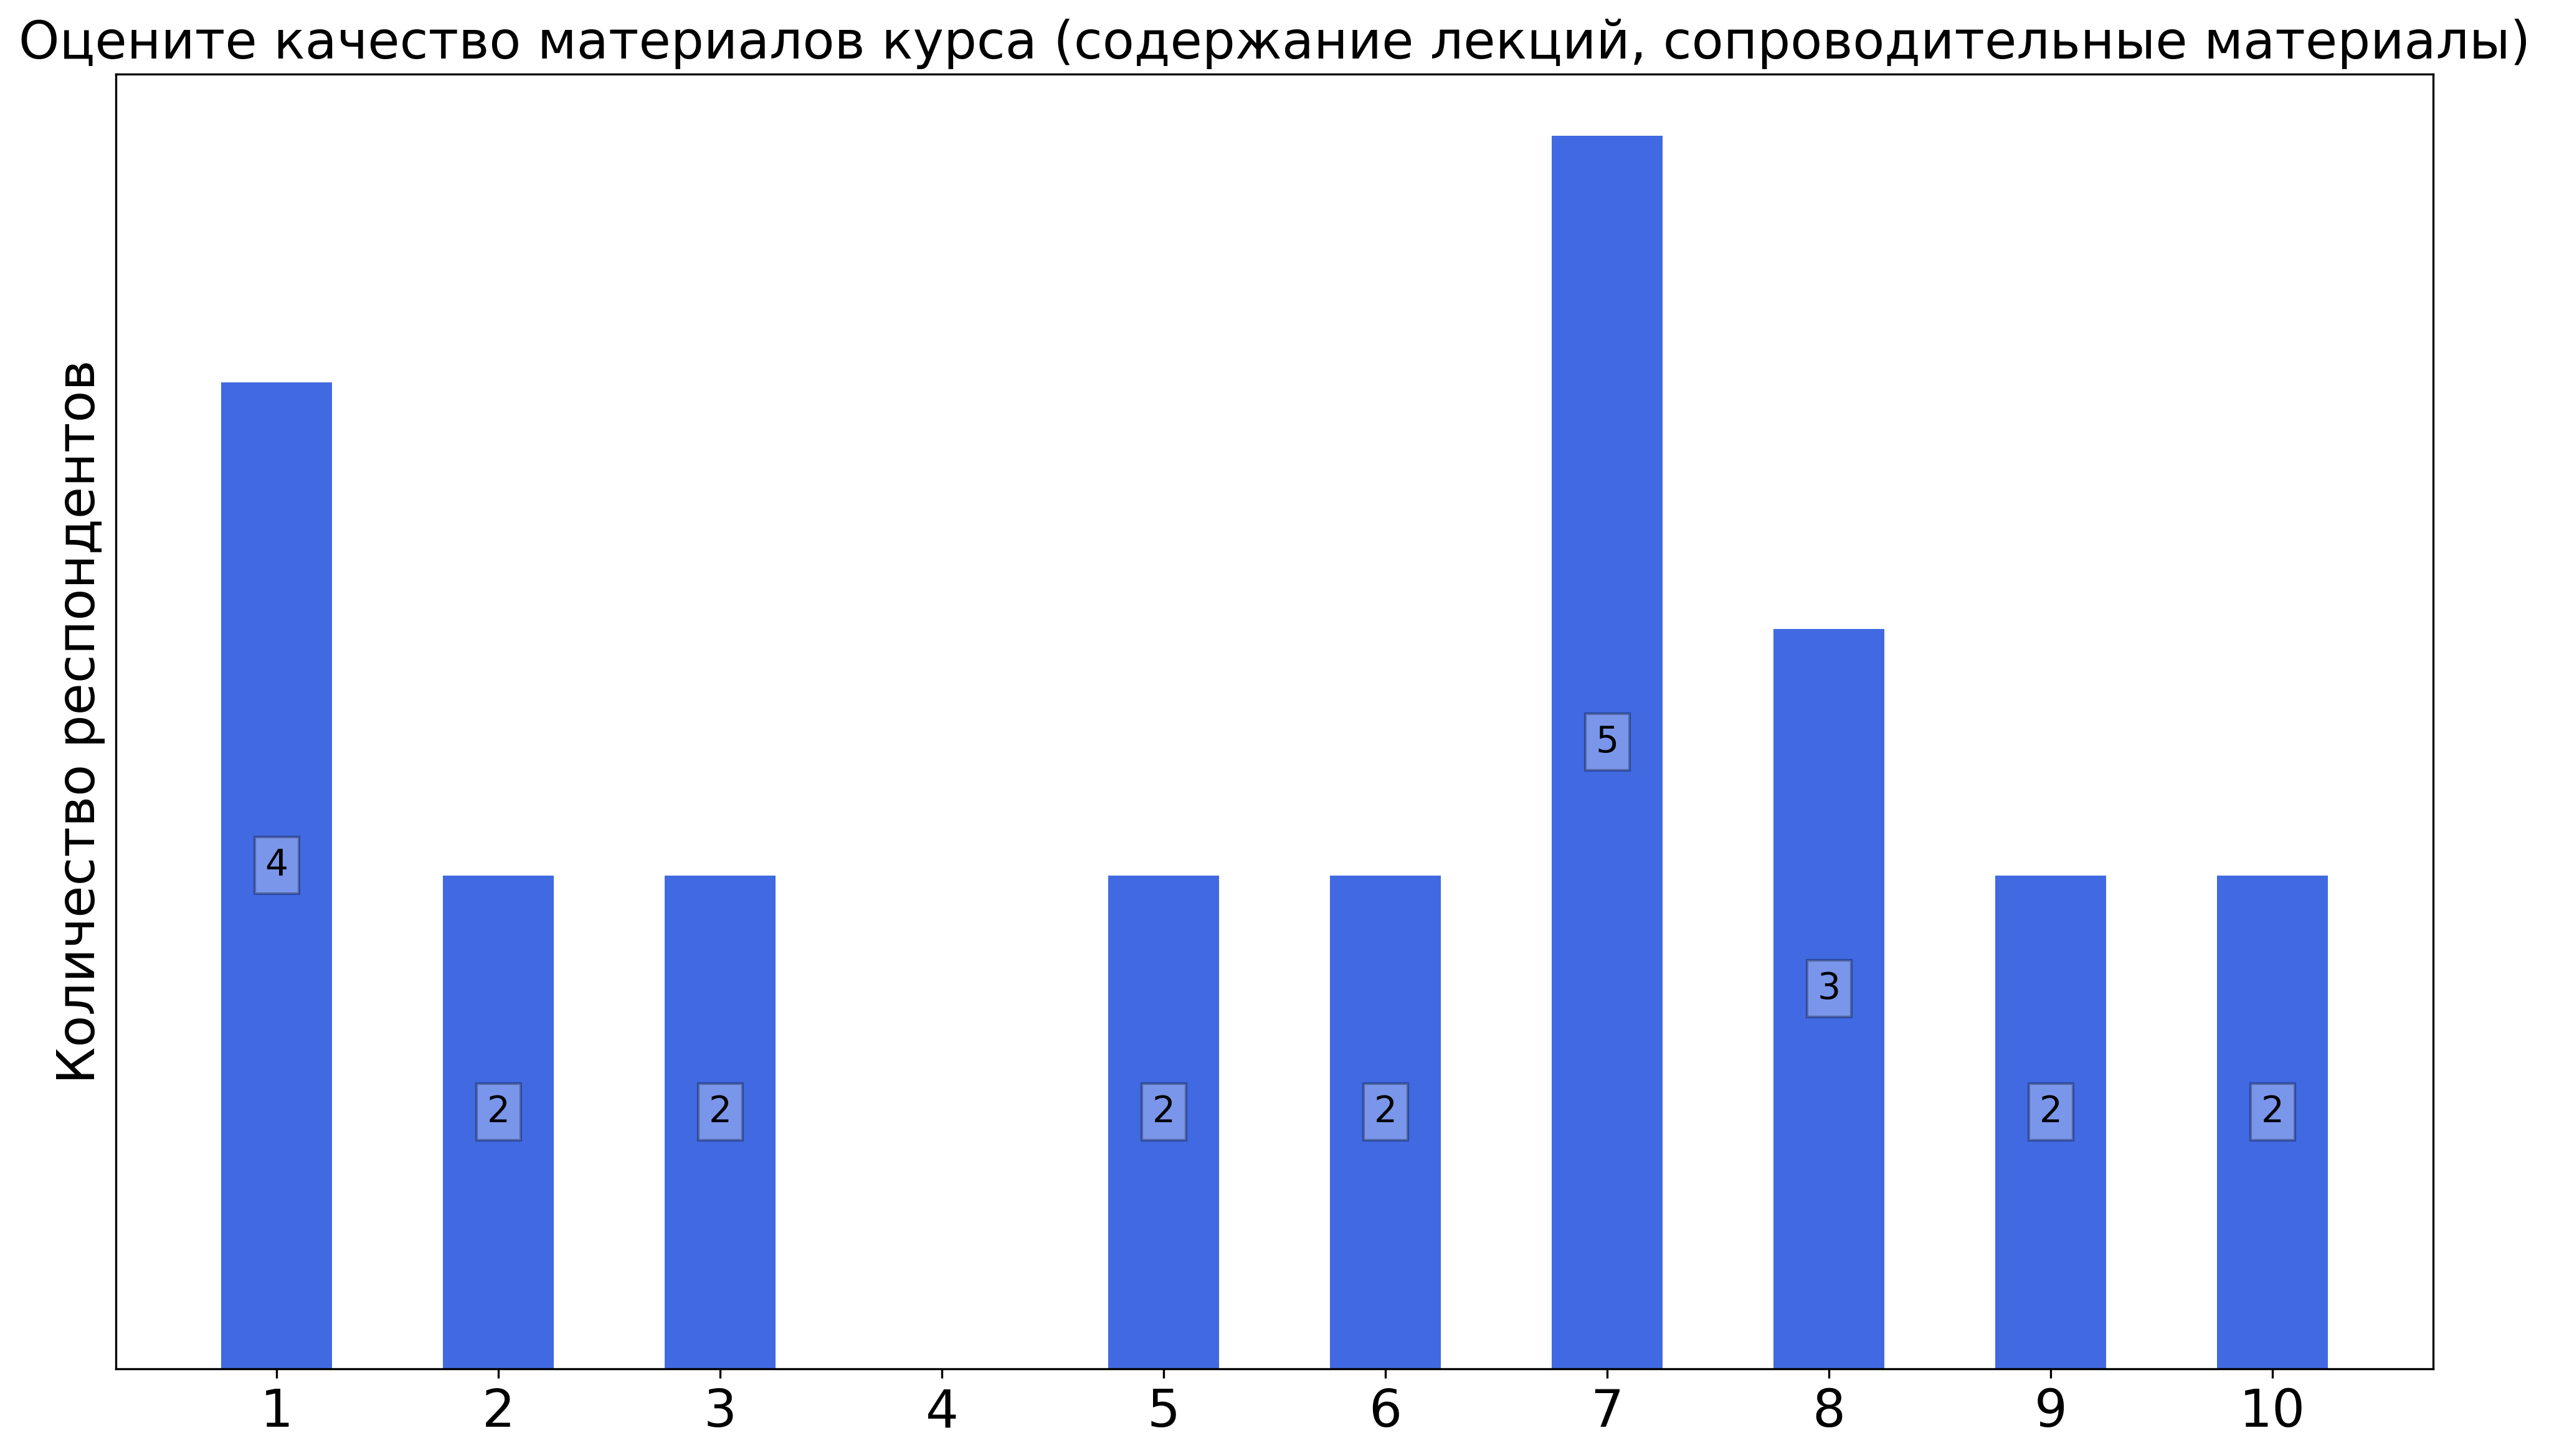
\includegraphics[width=\textwidth]{images/3 course/Общая физика - квантовая физика/lecturer-marks-Кобякин А.С.-1.png}
                \end{subfigure}
                \begin{subfigure}[b]{0.45\textwidth}
                    \centering
                    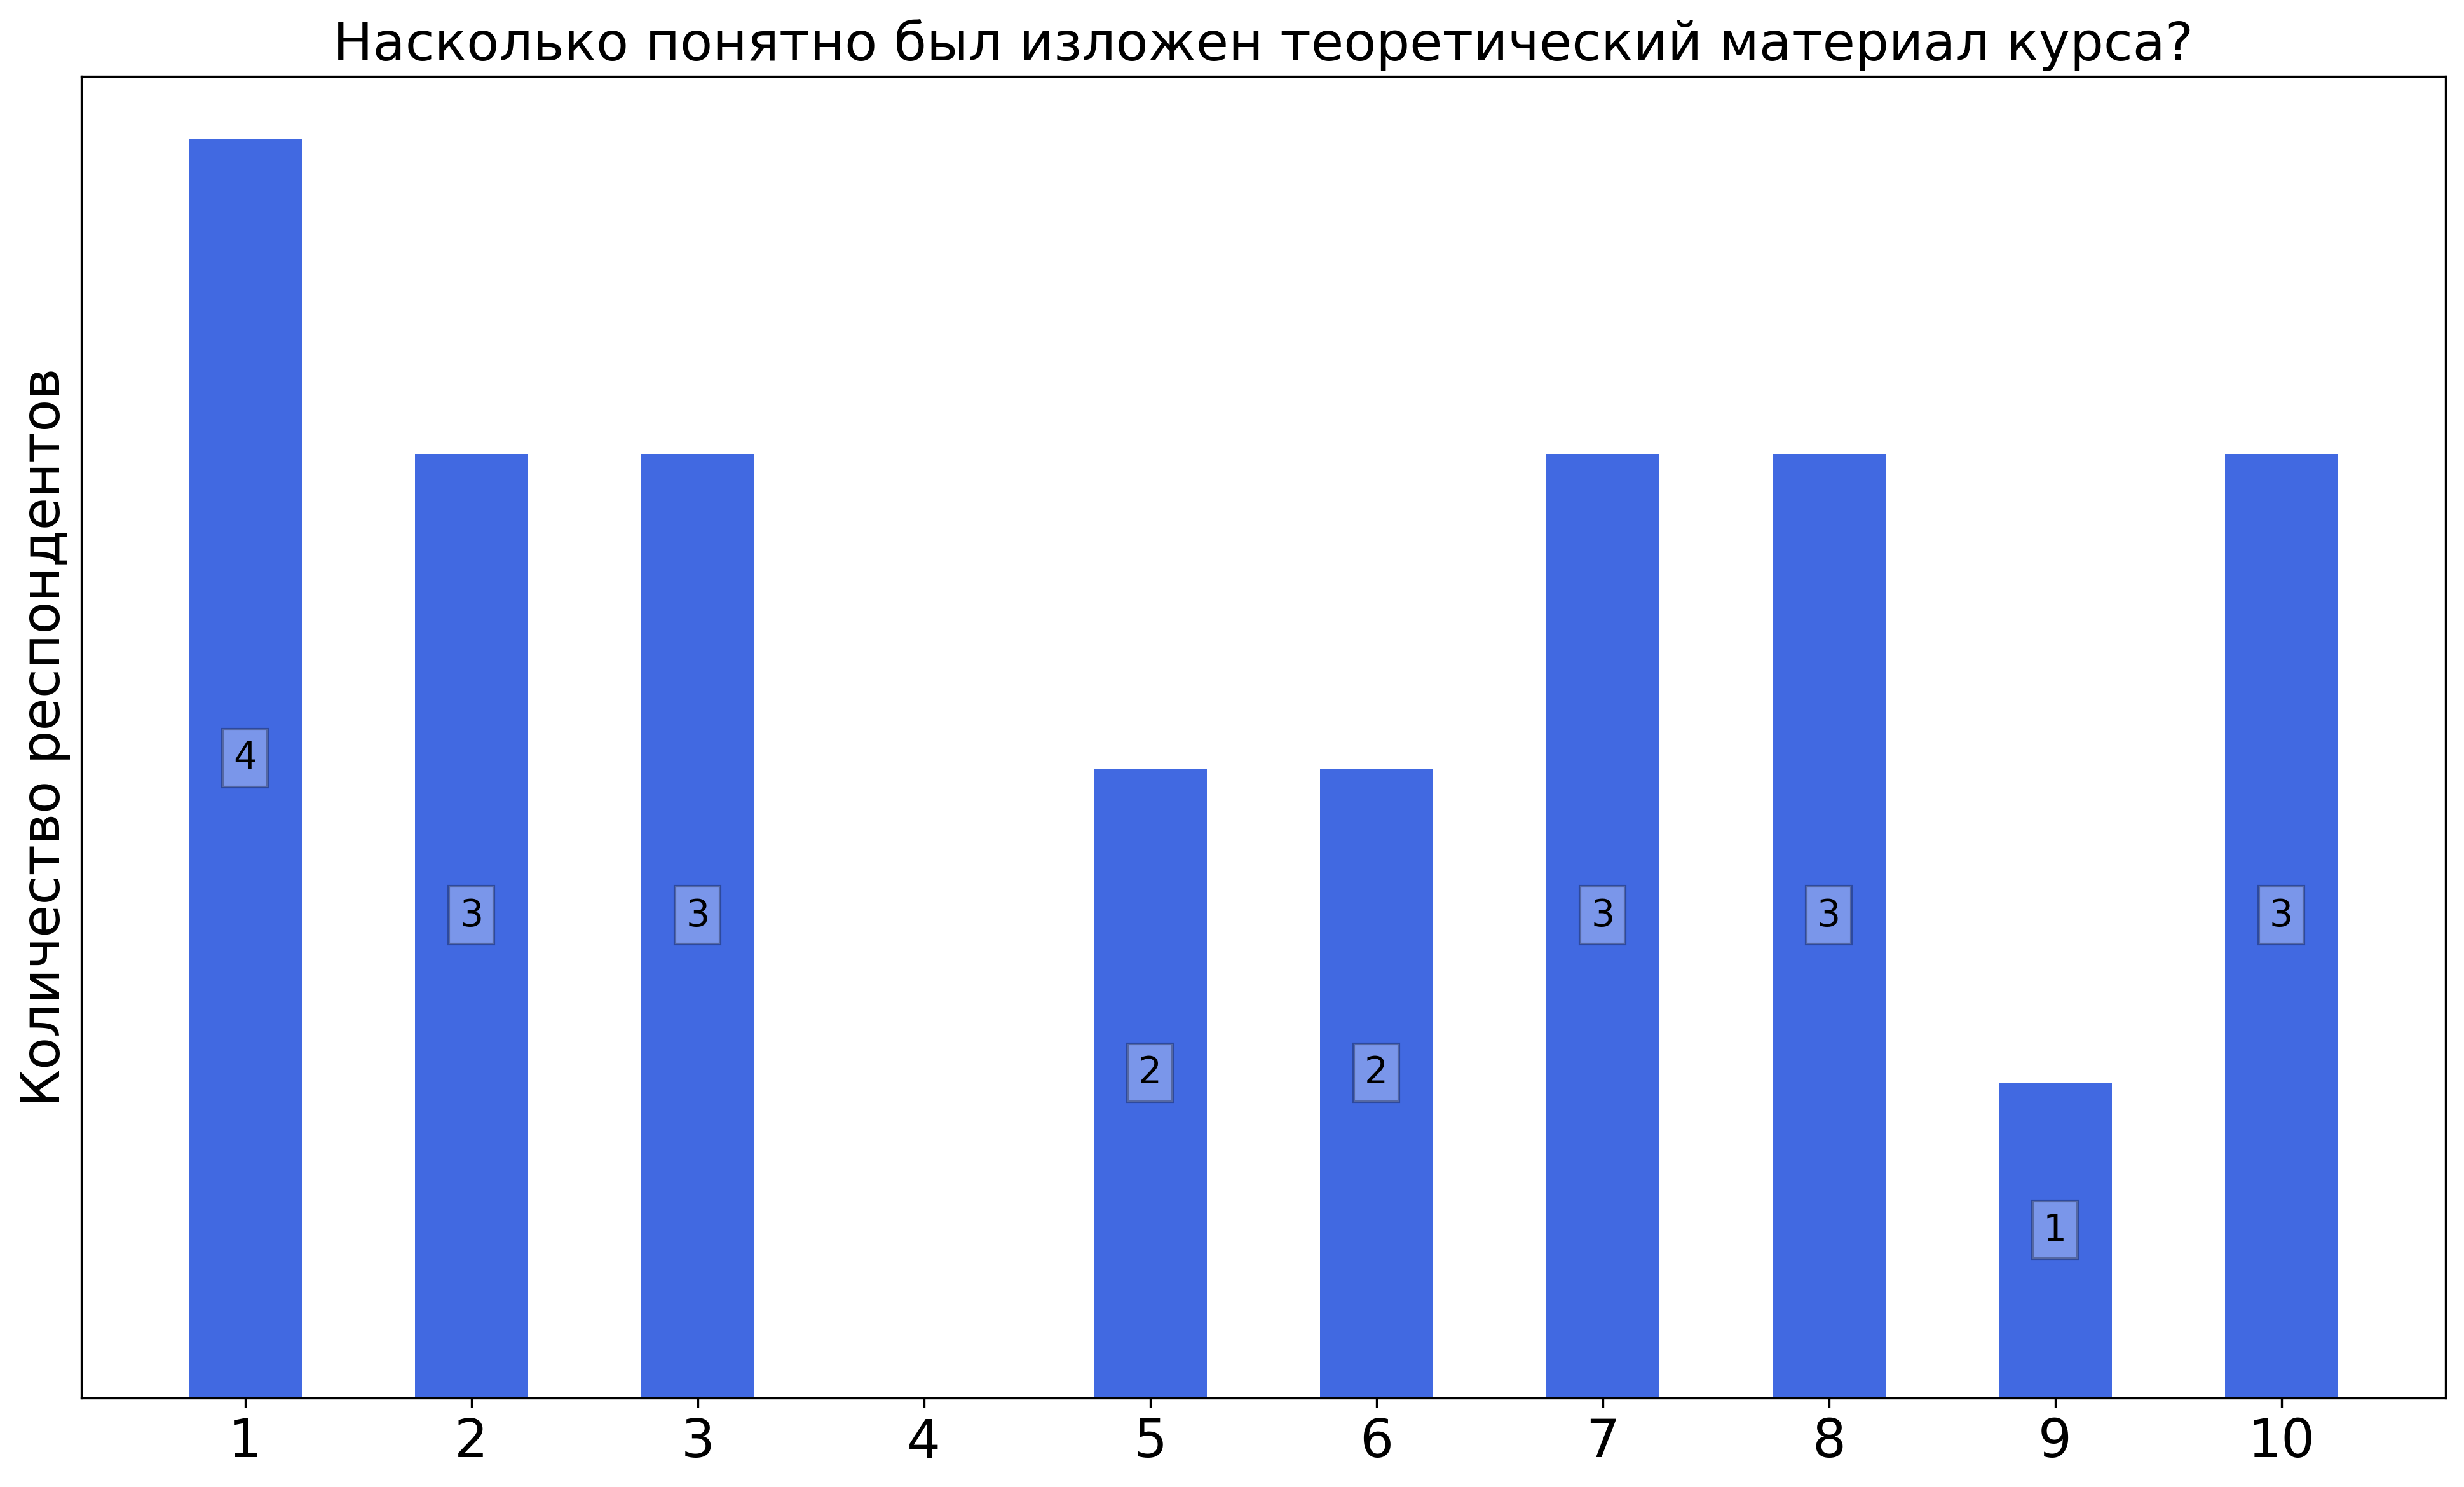
\includegraphics[width=\textwidth]{images/3 course/Общая физика - квантовая физика/lecturer-marks-Кобякин А.С.-2.png}
                \end{subfigure}	
                \begin{subfigure}[b]{0.45\textwidth}
                    \centering
                    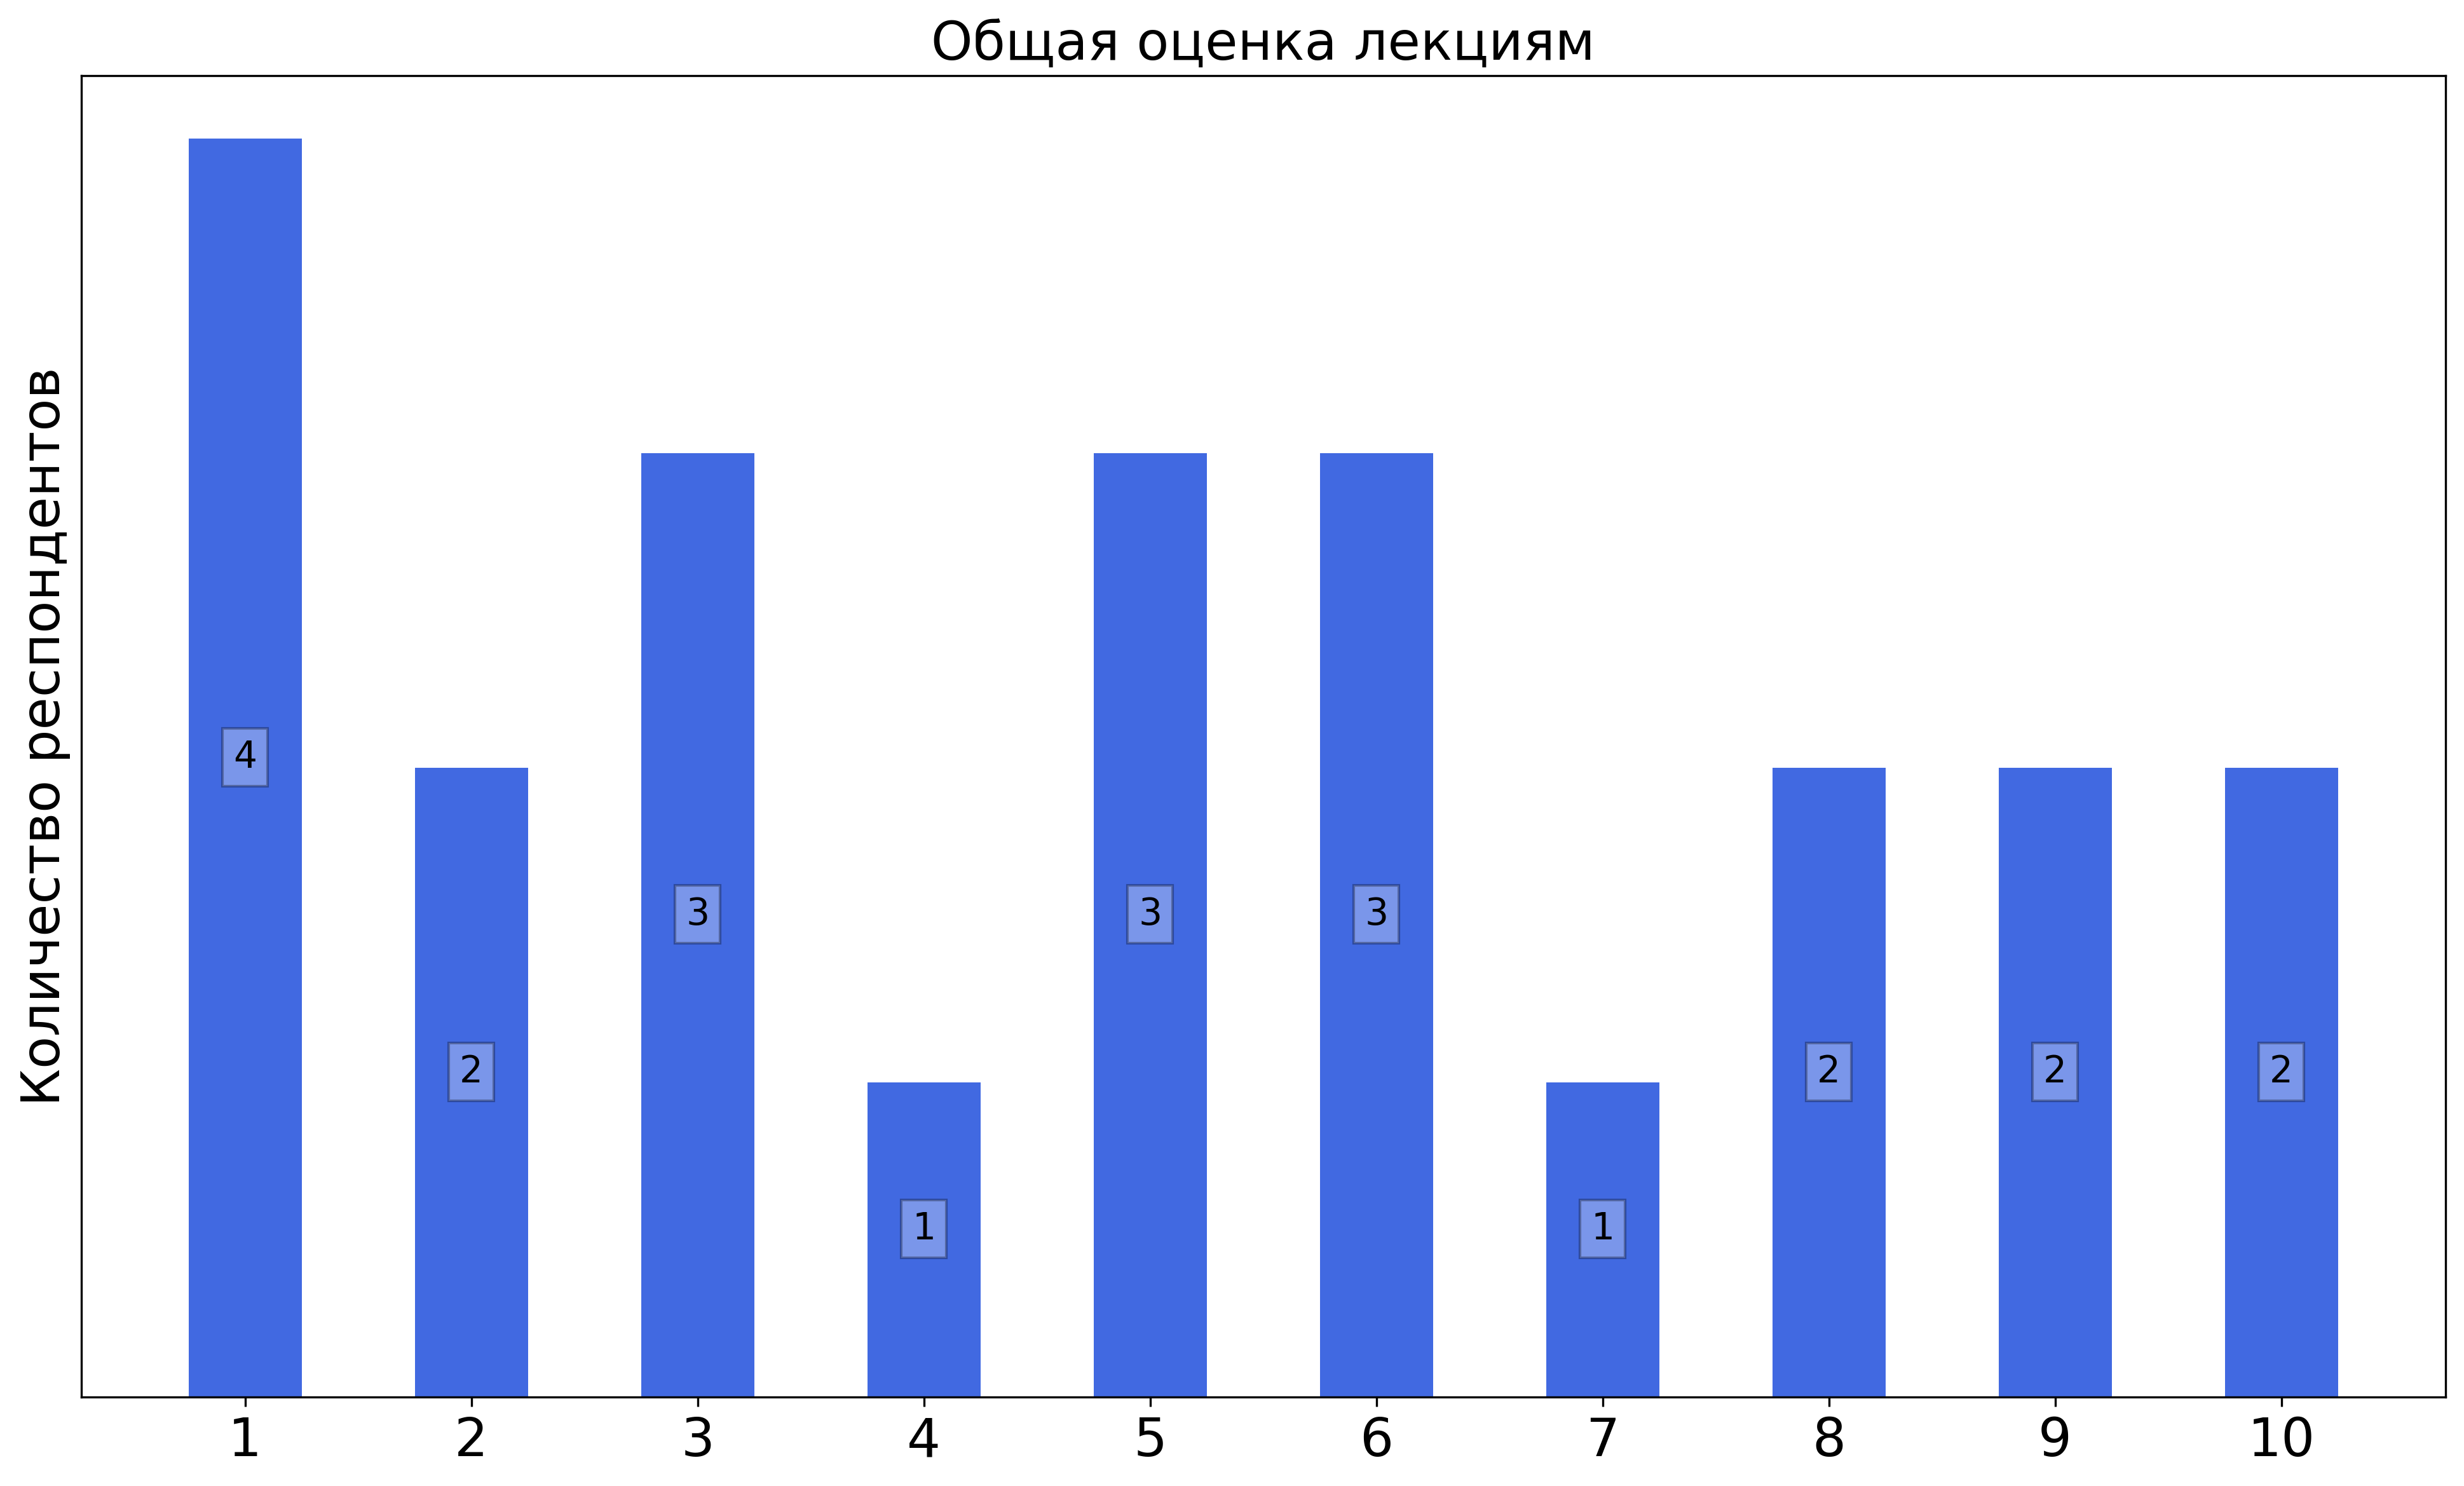
\includegraphics[width=\textwidth]{images/3 course/Общая физика - квантовая физика/lecturer-marks-Кобякин А.С.-3.png}
                \end{subfigure}
                \caption{Оценки респондентов о качестве преподавания лекций по курсу <<Общая физика: квантовая физика>>}
            \end{figure}

            \textbf{Комментарии студентов о лекциях\protect\footnote{сохранены оригинальные орфография и пунктуация}}
                \begin{commentbox} 
                    Не ходил, но то, что слышал: студентам не нравилось, как лектор читает. Не вникал в доказательства, а поверхностно проходился по каким-то азам 
                \end{commentbox} 
            
                \begin{commentbox} 
                    Смотрел Глазкова 
                \end{commentbox} 
            
                \begin{commentbox} 
                    не было структуры 
                \end{commentbox} 
            
                \begin{commentbox} 
                    Не понравилось, что очень смутно читает. На первых двух лекциях вообще ноль структуры, поэтому перестал ходить
                
                \end{commentbox} 
            
                \begin{commentbox} 
                    Абсолютно неструктурированное изложение материала. Походит на вброс рандомных фактов из физики, как будто человек просто хочет похвастаться знаниями. Лектор предполагает, что многие вещи нам очевидны со школы, но забывает, что уровень подготовки у всех разный. Говорит быстро и скомкано 
                \end{commentbox} 
            
                \begin{commentbox} 
                    Я не посещал много лекций для объективной оценки, но после первой лекции перестал ходить, потому что очень неструктурированное изложение материала. На первой лекции доска почти не использовалась. 
                \end{commentbox} 
            
                \begin{commentbox} 
                    Смотрел лекции и допсемы овчинкина, классный лектор и семинарист 
                \end{commentbox} 
            
                \begin{commentbox} 
                    лекции крайне слабы: лектор перескакивает с темы на тему, говорит слишком нечетко, на вопросы отвечает неконструктивно
            
                    Смотрел записи лекций 2021года В Н Глазкова - отличные! 
                \end{commentbox} 
            
                \begin{commentbox} 
                    Первая лекция была просто набором рандомных фактов, связанных со столкновением частиц и т.п. Никакой структуры не почувствовал и следовательно ничего с нее не запомнил. После первой же лекции перешел на Гаврикова, ну а Гавриков топ 
                \end{commentbox} 
            
                \begin{commentbox} 
                    Глазкова В. Н. - великолепин. 
                    У Кобякина А. С. был на первой лекции - не понравилось. Мне не хватило структурности. 
                \end{commentbox} 
            
                \begin{commentbox} 
                    На первой лекции изначально была непонятна логика повествования: куда лектор ведёт? Что хочет донести? И вообще у него аура недружелюбная. Поэтому лучшим выходом было смотреть видео лекции легендарного Андрея Владимировича Гаврикова) 
                \end{commentbox} 

                \begin{commentbox} 
                    Глазков moment 
                \end{commentbox} 
            
                \begin{commentbox} 
                    Был на одной лекции, которая напрочь отбила желание посещать последующее. До этого на протяжении 4 семестров общей физики ходил почти на все лекции. Лектор, вместо последовательного изложения материал, задавал аудитории множество вопросов, ожидая, что студенты сами на них ответят. Сама же лекция была жутко неструктурированной, на ней ничего не было понятно. В итоге смотрел записанные лекции Гаврикова. 
                \end{commentbox} 
            
                \begin{commentbox} 
                    Любимые цитаты Кобякина полностью отбили желание даже слушать такого человека. По отзывам ходивших, лучше правда посмотреть глазкова, что я и сделал. 
                \end{commentbox} 
        
        
        \subsubsection{Отзыв студентов о семинарах. Семинарист: Аникин Ю.А.}
            \begin{figure}[H]
                \centering
                \begin{subfigure}[b]{0.45\textwidth}
                    \centering
                    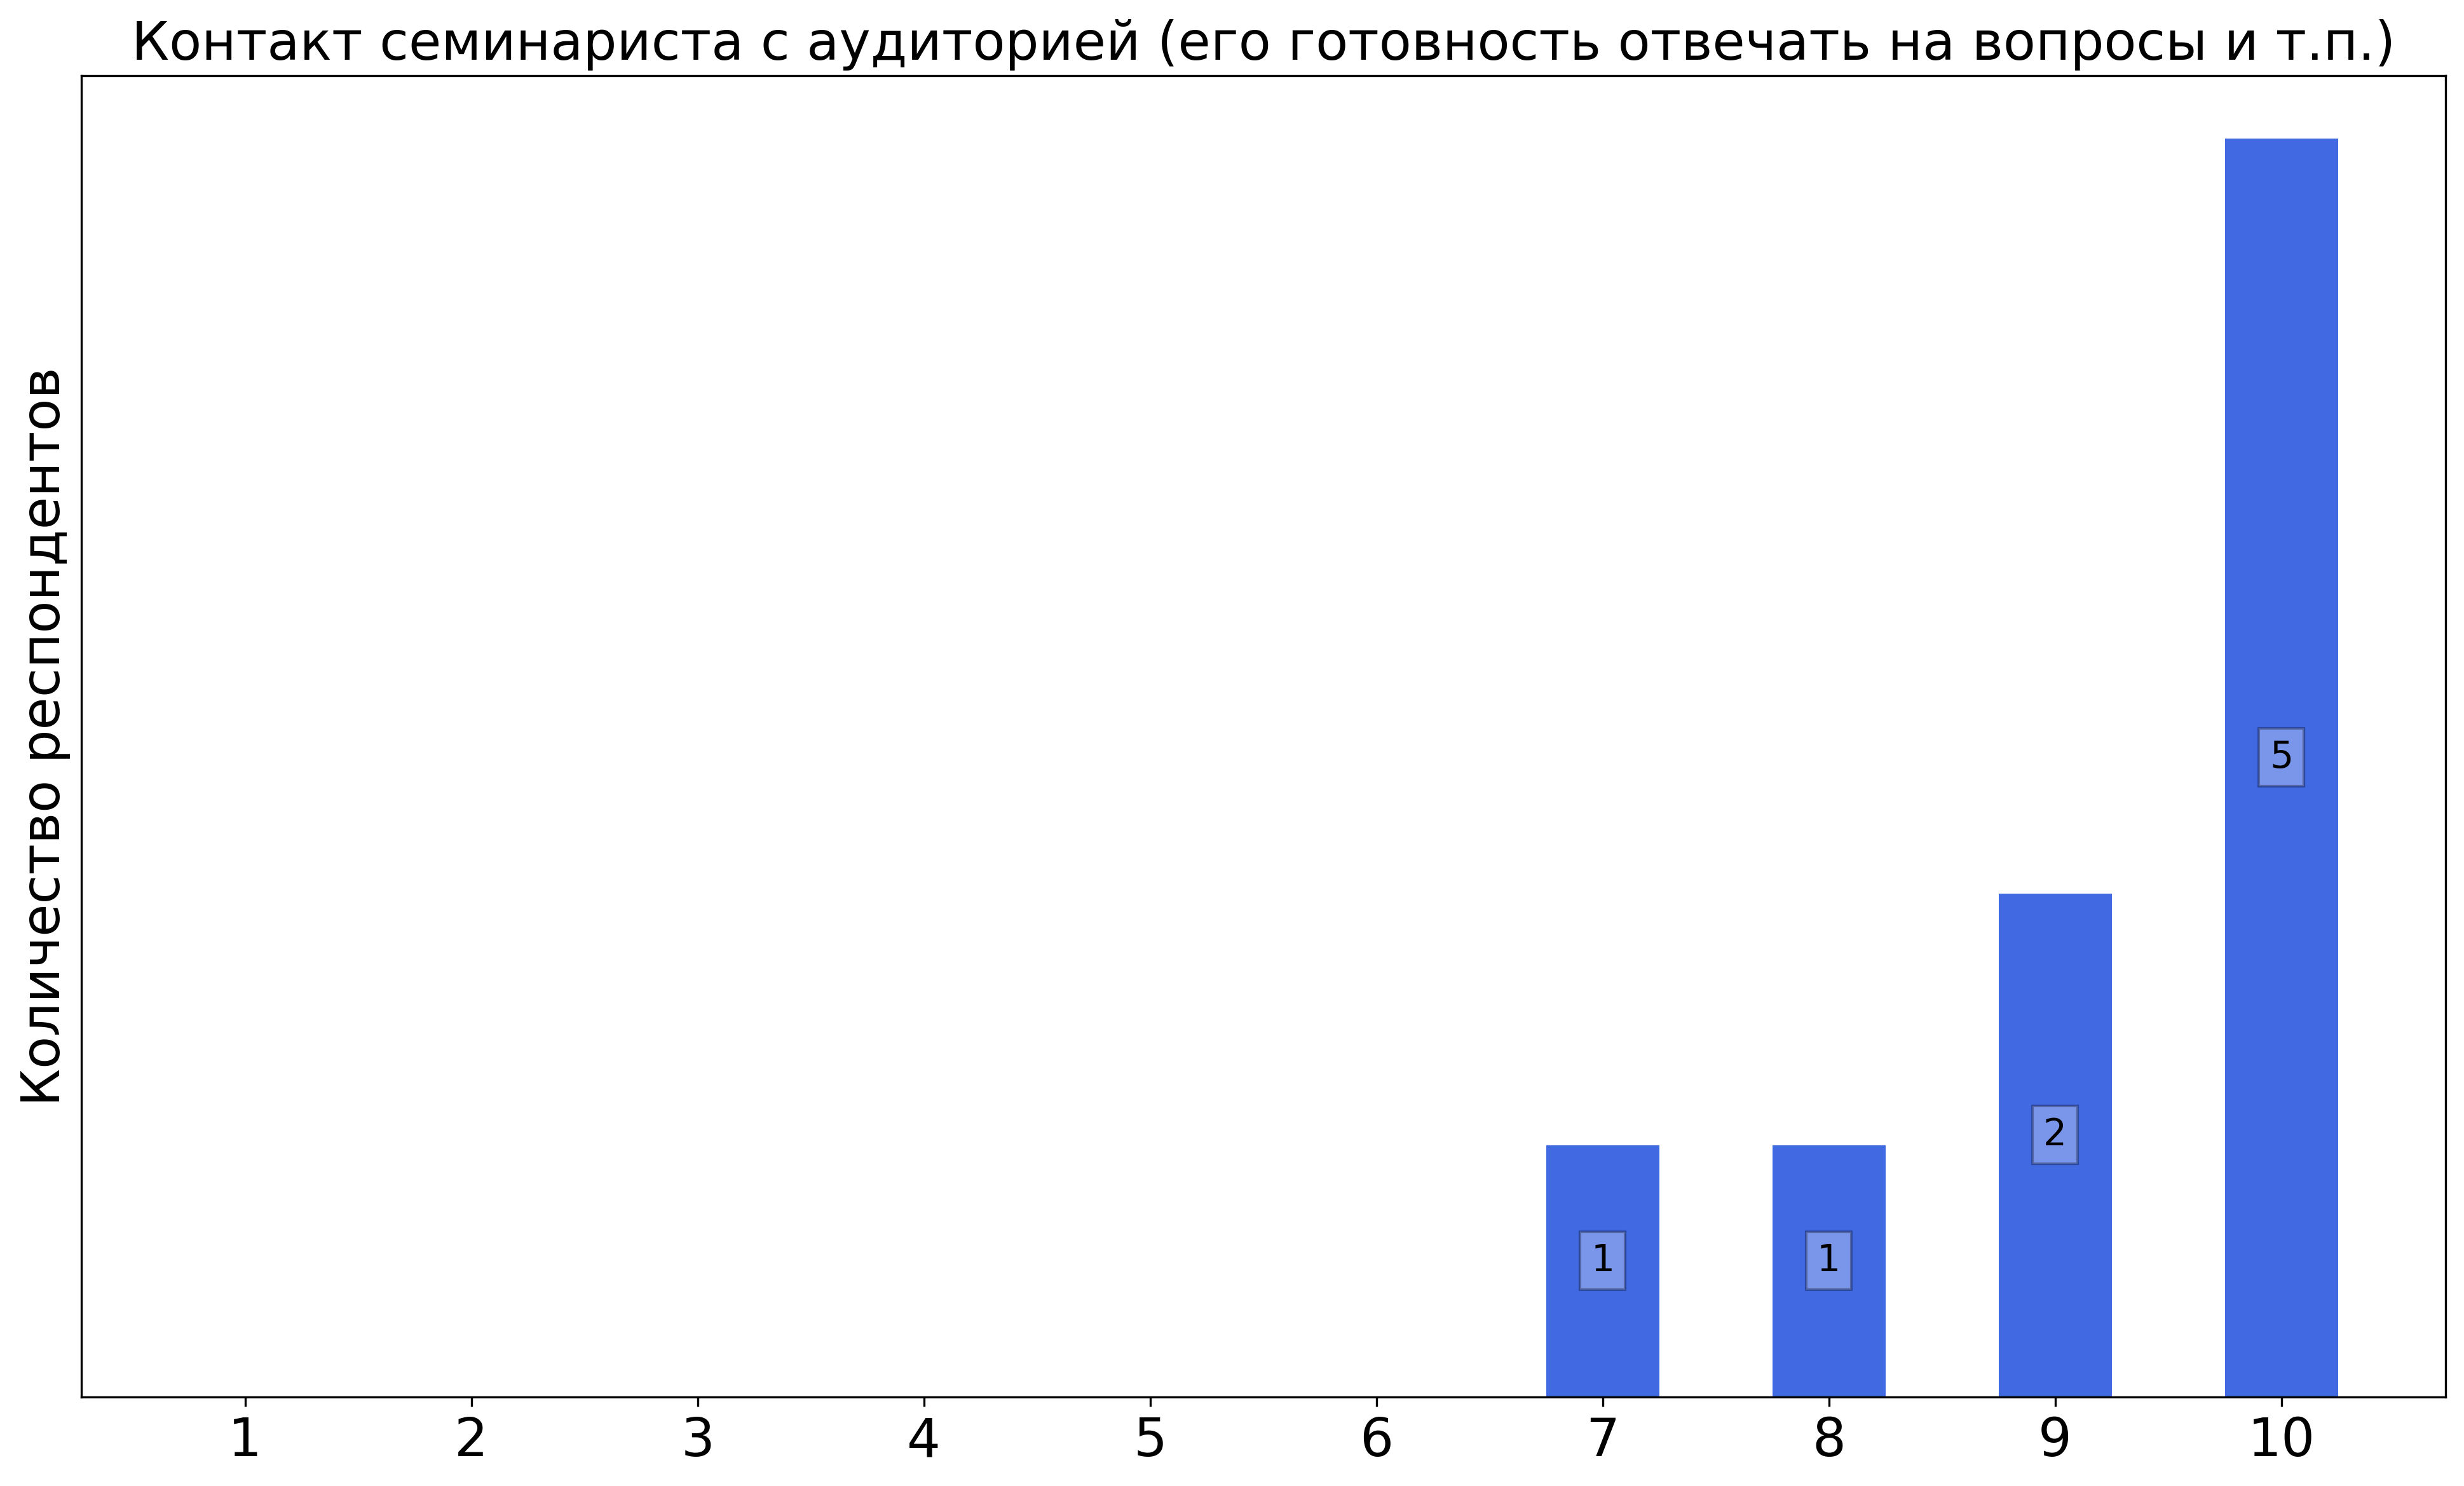
\includegraphics[width=\textwidth]{images/3 course/Общая физика - квантовая физика/seminarists-marks-Аникин Ю.А.-0.png}
                \end{subfigure}
                \begin{subfigure}[b]{0.45\textwidth}
                    \centering
                    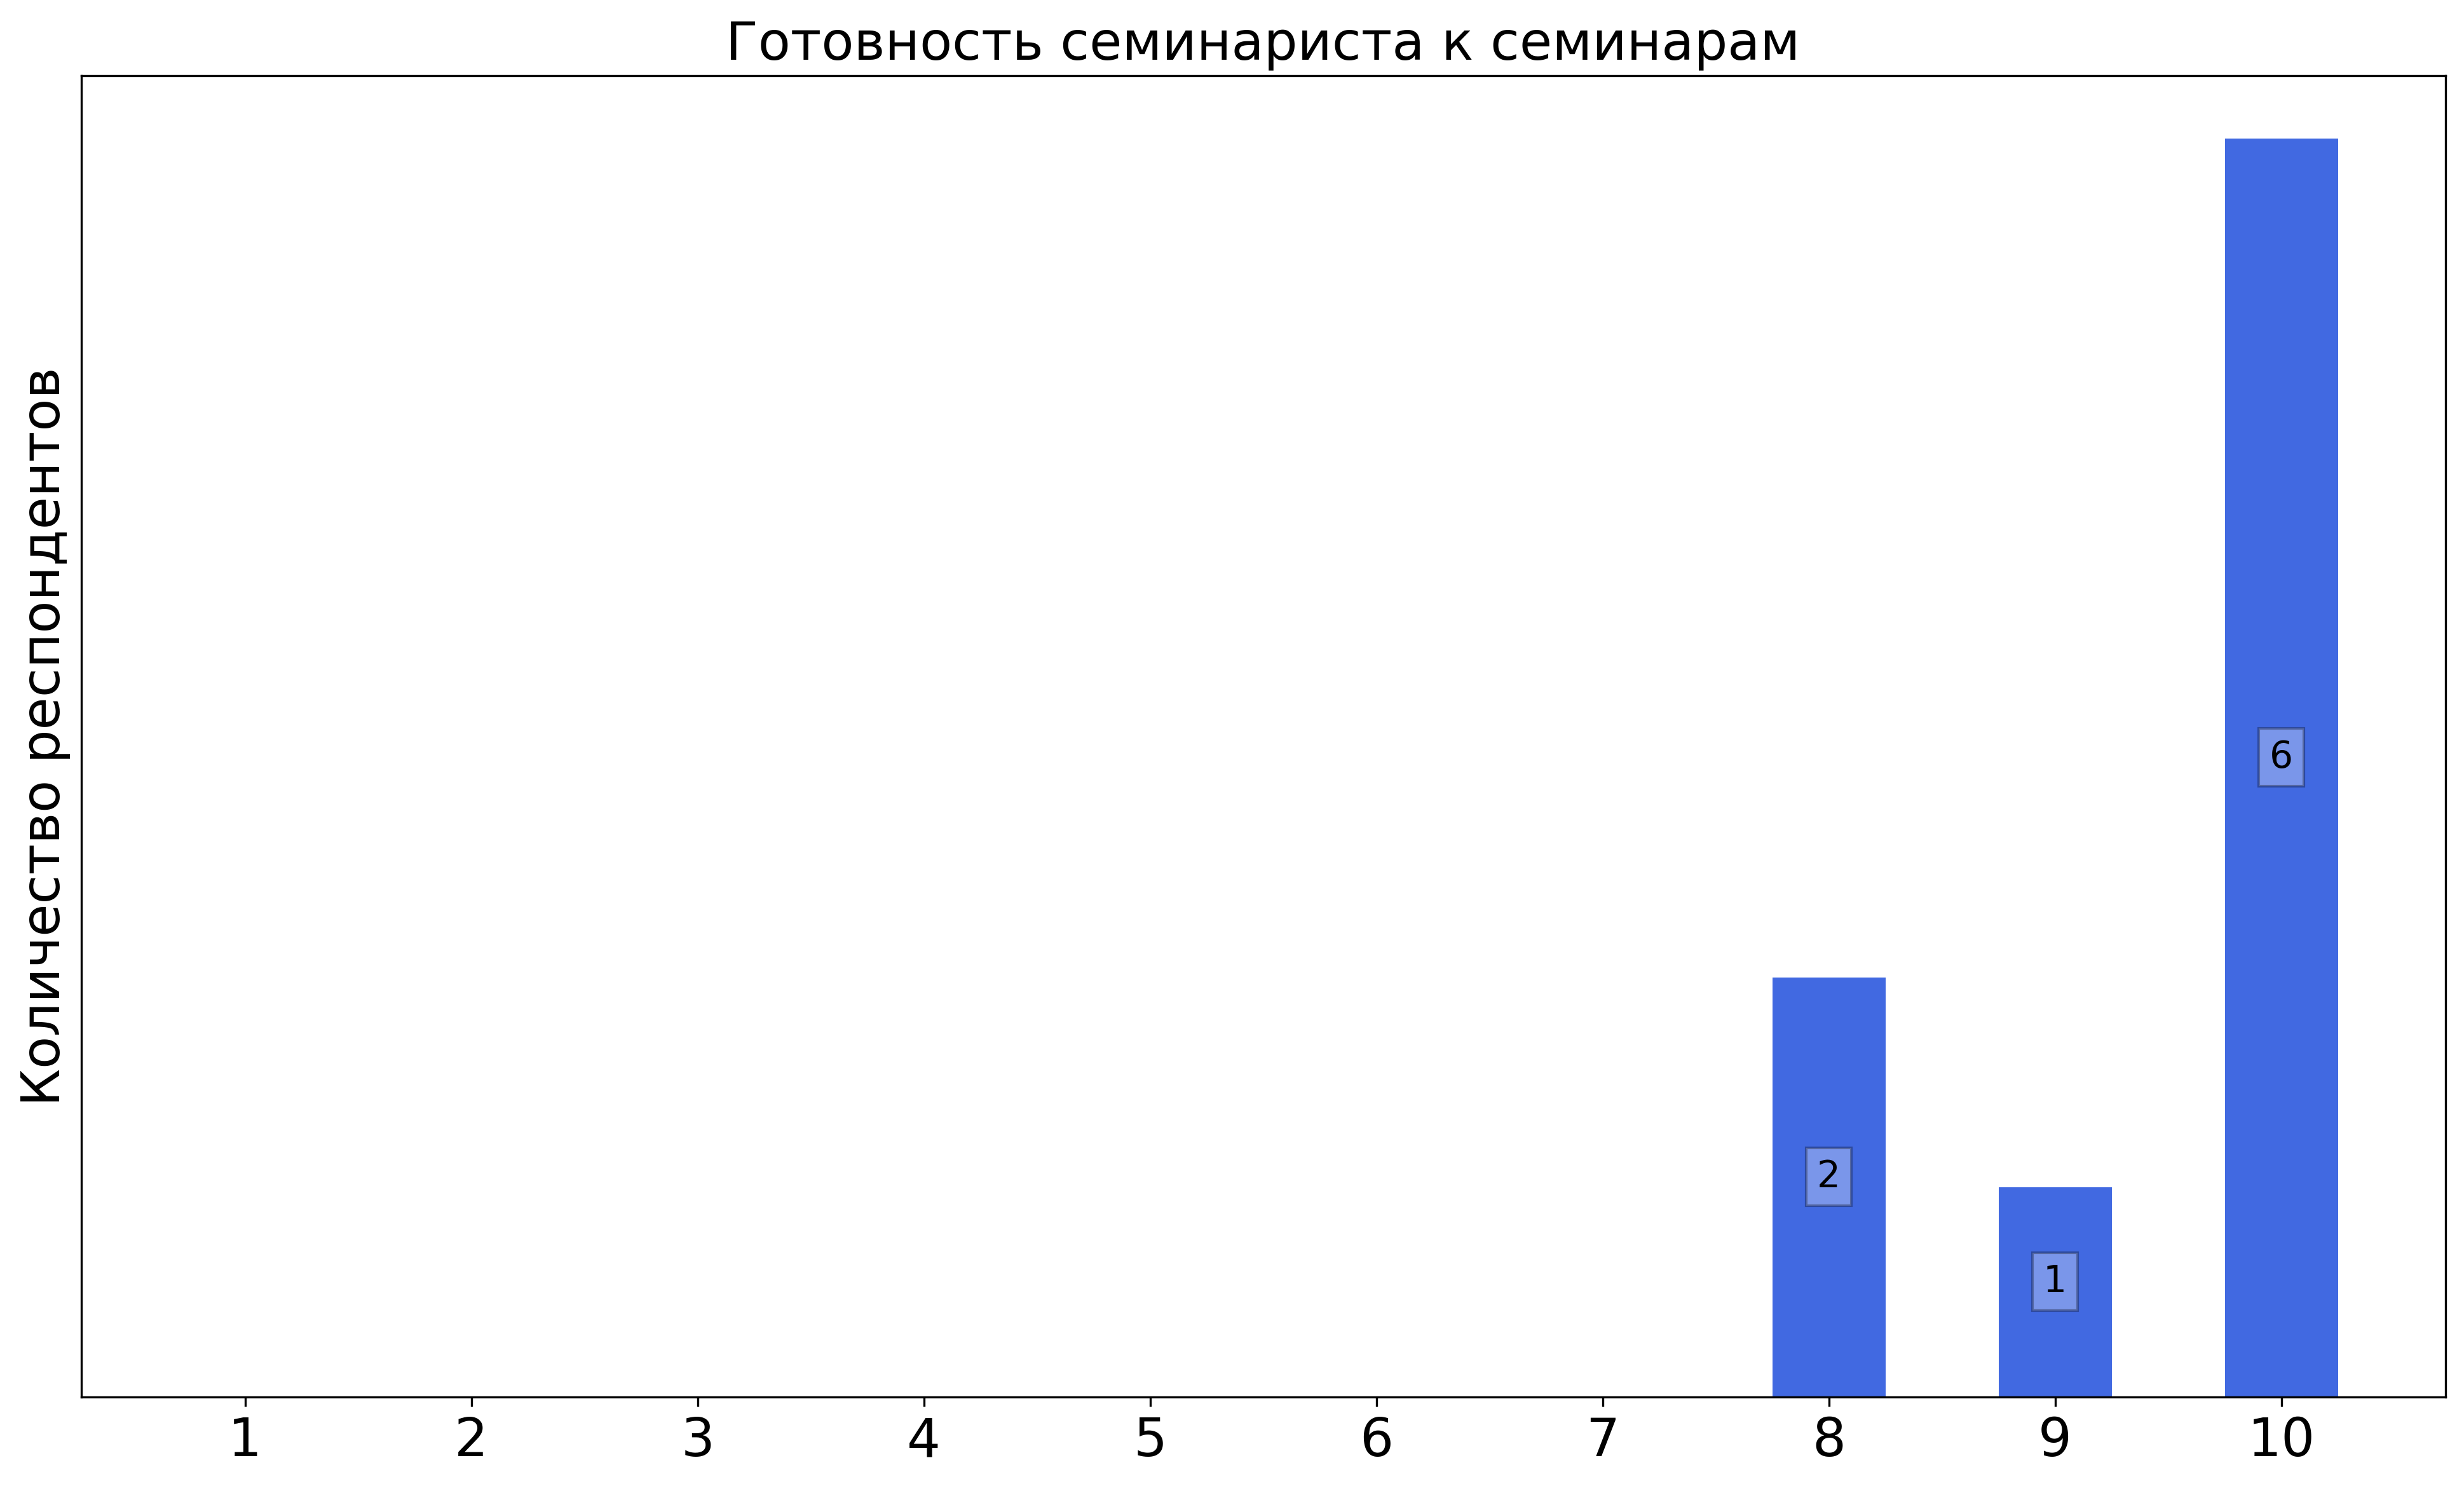
\includegraphics[width=\textwidth]{images/3 course/Общая физика - квантовая физика/seminarists-marks-Аникин Ю.А.-1.png}
                \end{subfigure}
                \begin{subfigure}[b]{0.45\textwidth}
                    \centering
                    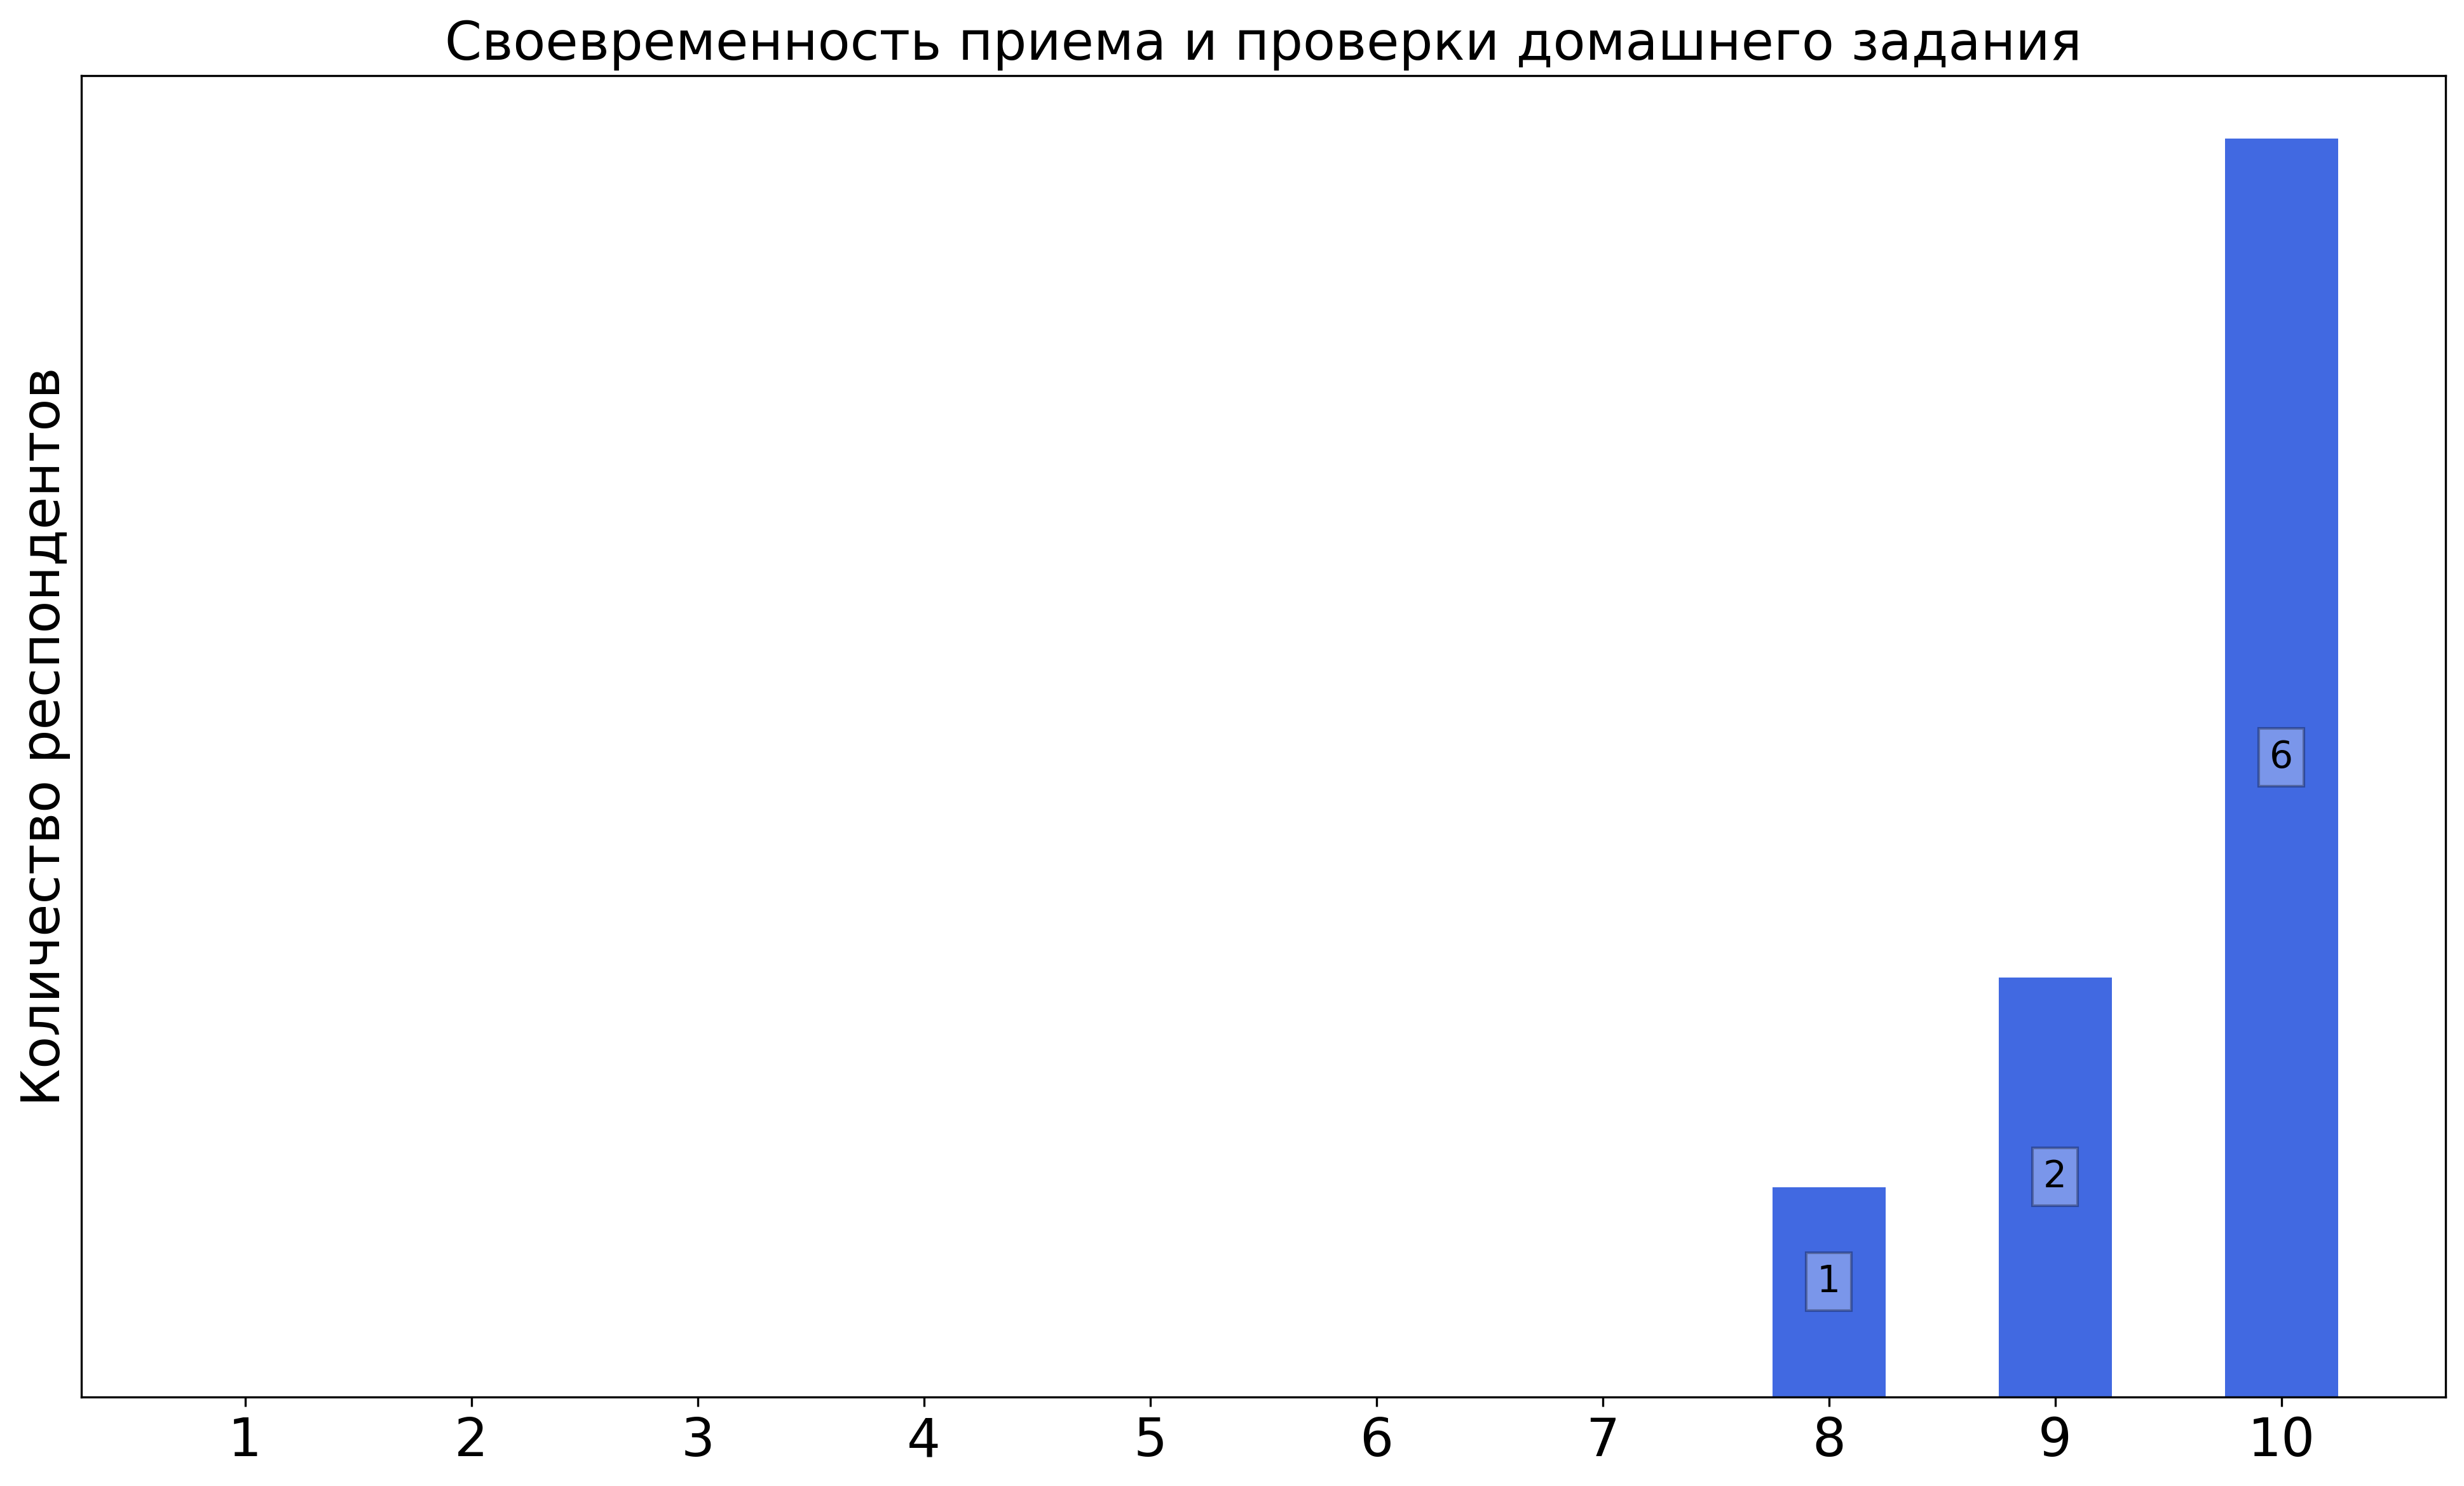
\includegraphics[width=\textwidth]{images/3 course/Общая физика - квантовая физика/seminarists-marks-Аникин Ю.А.-2.png}
                \end{subfigure}
                \begin{subfigure}[b]{0.45\textwidth}
                    \centering
                    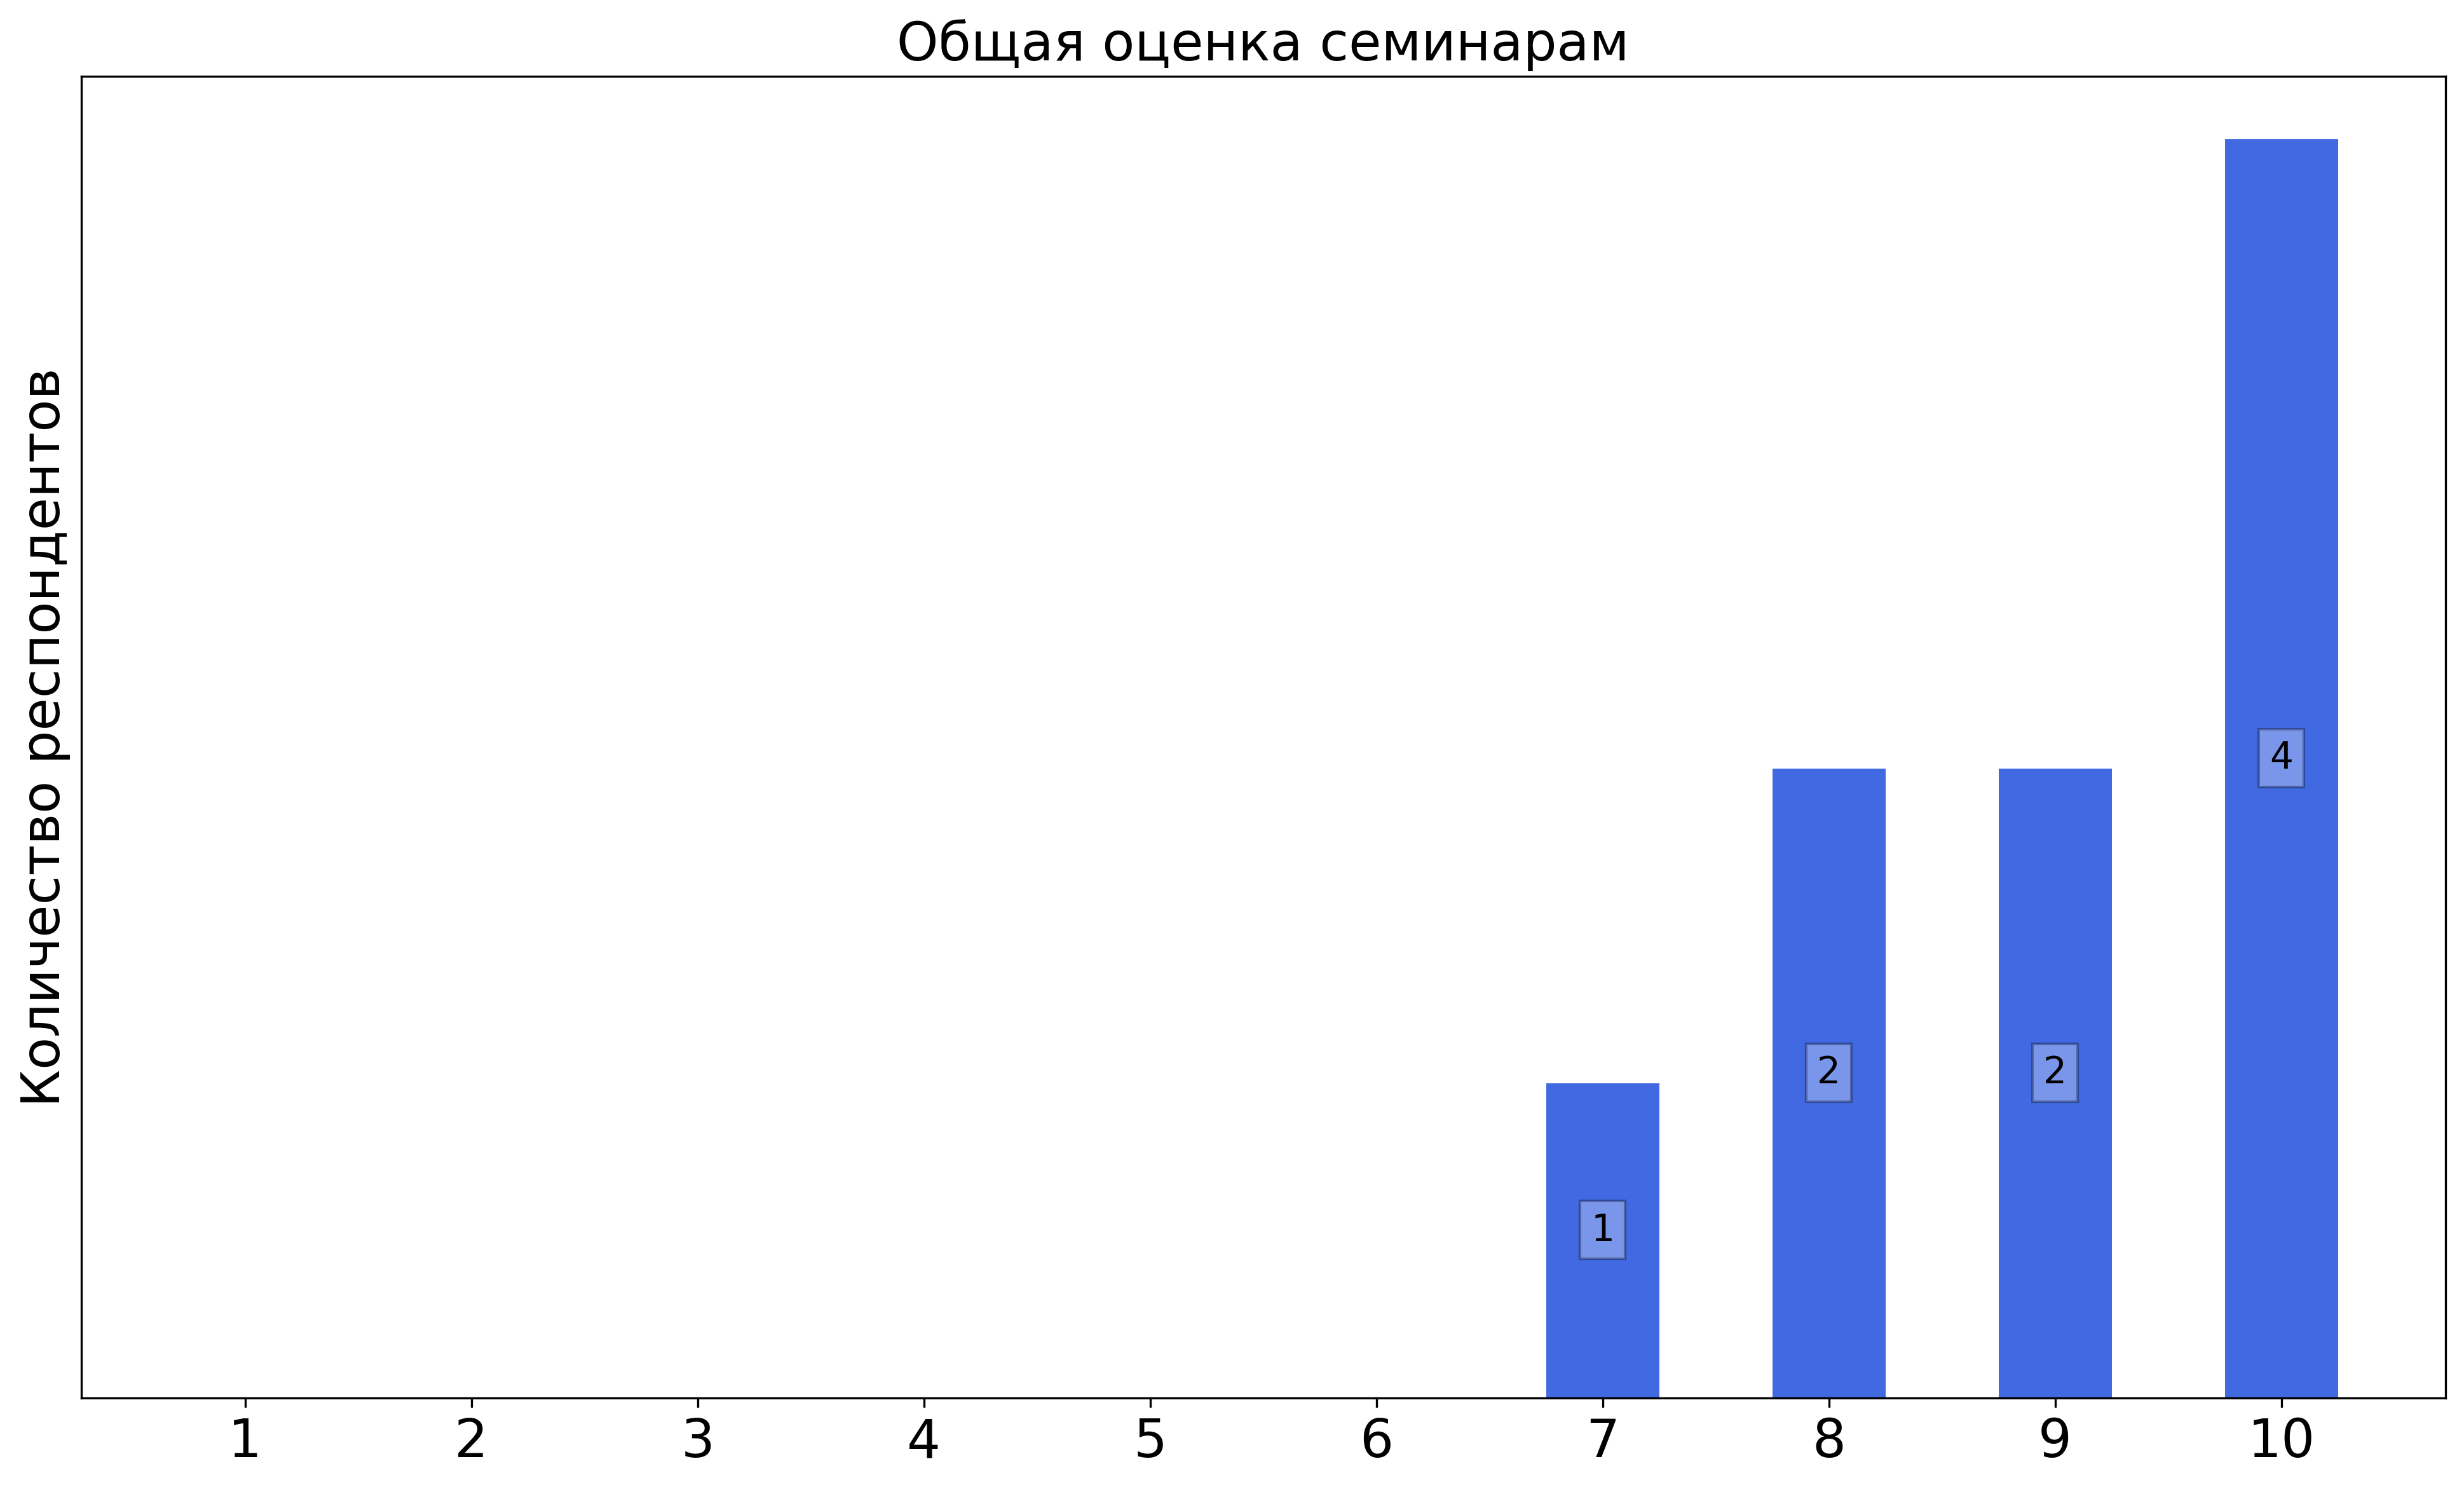
\includegraphics[width=\textwidth]{images/3 course/Общая физика - квантовая физика/seminarists-marks-Аникин Ю.А.-3.png}
                \end{subfigure}	
                \caption{Оценки респондентов о качестве преподавания семинаров}
            \end{figure}

            \textbf{Комментарии студентов о семинаристе\protect\footnote{сохранены оригинальные орфография и пунктуация}}
                \begin{commentbox} 
                    Очень сильно проглатывает слова, поэтому часто тяжело вникнуть в его рассказ. Очень часто обрывки рассказывает материал, из-за чего сложно собрать полную картину. 
                \end{commentbox} 
            
                \begin{commentbox} 
                    Один из лучших семинаристов за весь физтех. Отлично знает материал, готовится к семинарам. В начале семинара рассказывает теоретическую справку с небольшими реально интересными историческими справками. После переходит к задачам, которые всегда подготовлены на листочке, но он их знает наизусть. Если не все необходимые задачи были разобраны, то на словах рассказывает основные идеи, причем действительно понятно. Всегда шел на встречу,  не задерживал (у нас после него был Климанов), однажды начал семинар на 5 мин раньше по нашей просьбе, чтобы раньше отпустить. Бывают странные шутки, понятные только сильным фанатам вархамера/игры престолов (это скорее минус). 
                \end{commentbox} 
            
                \begin{commentbox} 
                    Очень хороший семинарист, всё по делу, адекватные критерии оценивания. Все его боялись,а он превзошел все ожидания!! 
                \end{commentbox} 
            
                \begin{commentbox} 
                    Лучший семинарист за 5 семестров. Расшаривает, очень неплохо объясняет, помогает разобраться. Отностельно других преподавателей кафедры принимает задание довольно строго, но, если делаешь сам, то проблем со сдачей не будет. Очень понравились семинары, спасибо за самый интересный семестр общей физики на Физтехе! 
                \end{commentbox} 
            
                \begin{commentbox} 
                    Хороший семинарист. Да, строже, чем среднестатистический, но зато получаешь отличный уровень подготовки по квантам к госу. Сдачи заданий в виде решения 4 задач из дз без использования доп материалов позволили классно зашарить. 
                \end{commentbox} 
            
                \begin{commentbox} 
                    Семинарист хороший, объясняет понятно, с интересом, с готовностью отвечает на вопросы, действительно хочет добиться понимания темы. Оценивает абсолютно адекватно, хотя сдачи заданий - довольно неприятный процесс, но оценкой не обижает.
                \end{commentbox} 


        \subsubsection{Отзыв студентов о семинарах. Семинарист: Виноградов С.В.}
            \begin{figure}[H]
                \centering
                \begin{subfigure}[b]{0.45\textwidth}
                    \centering
                    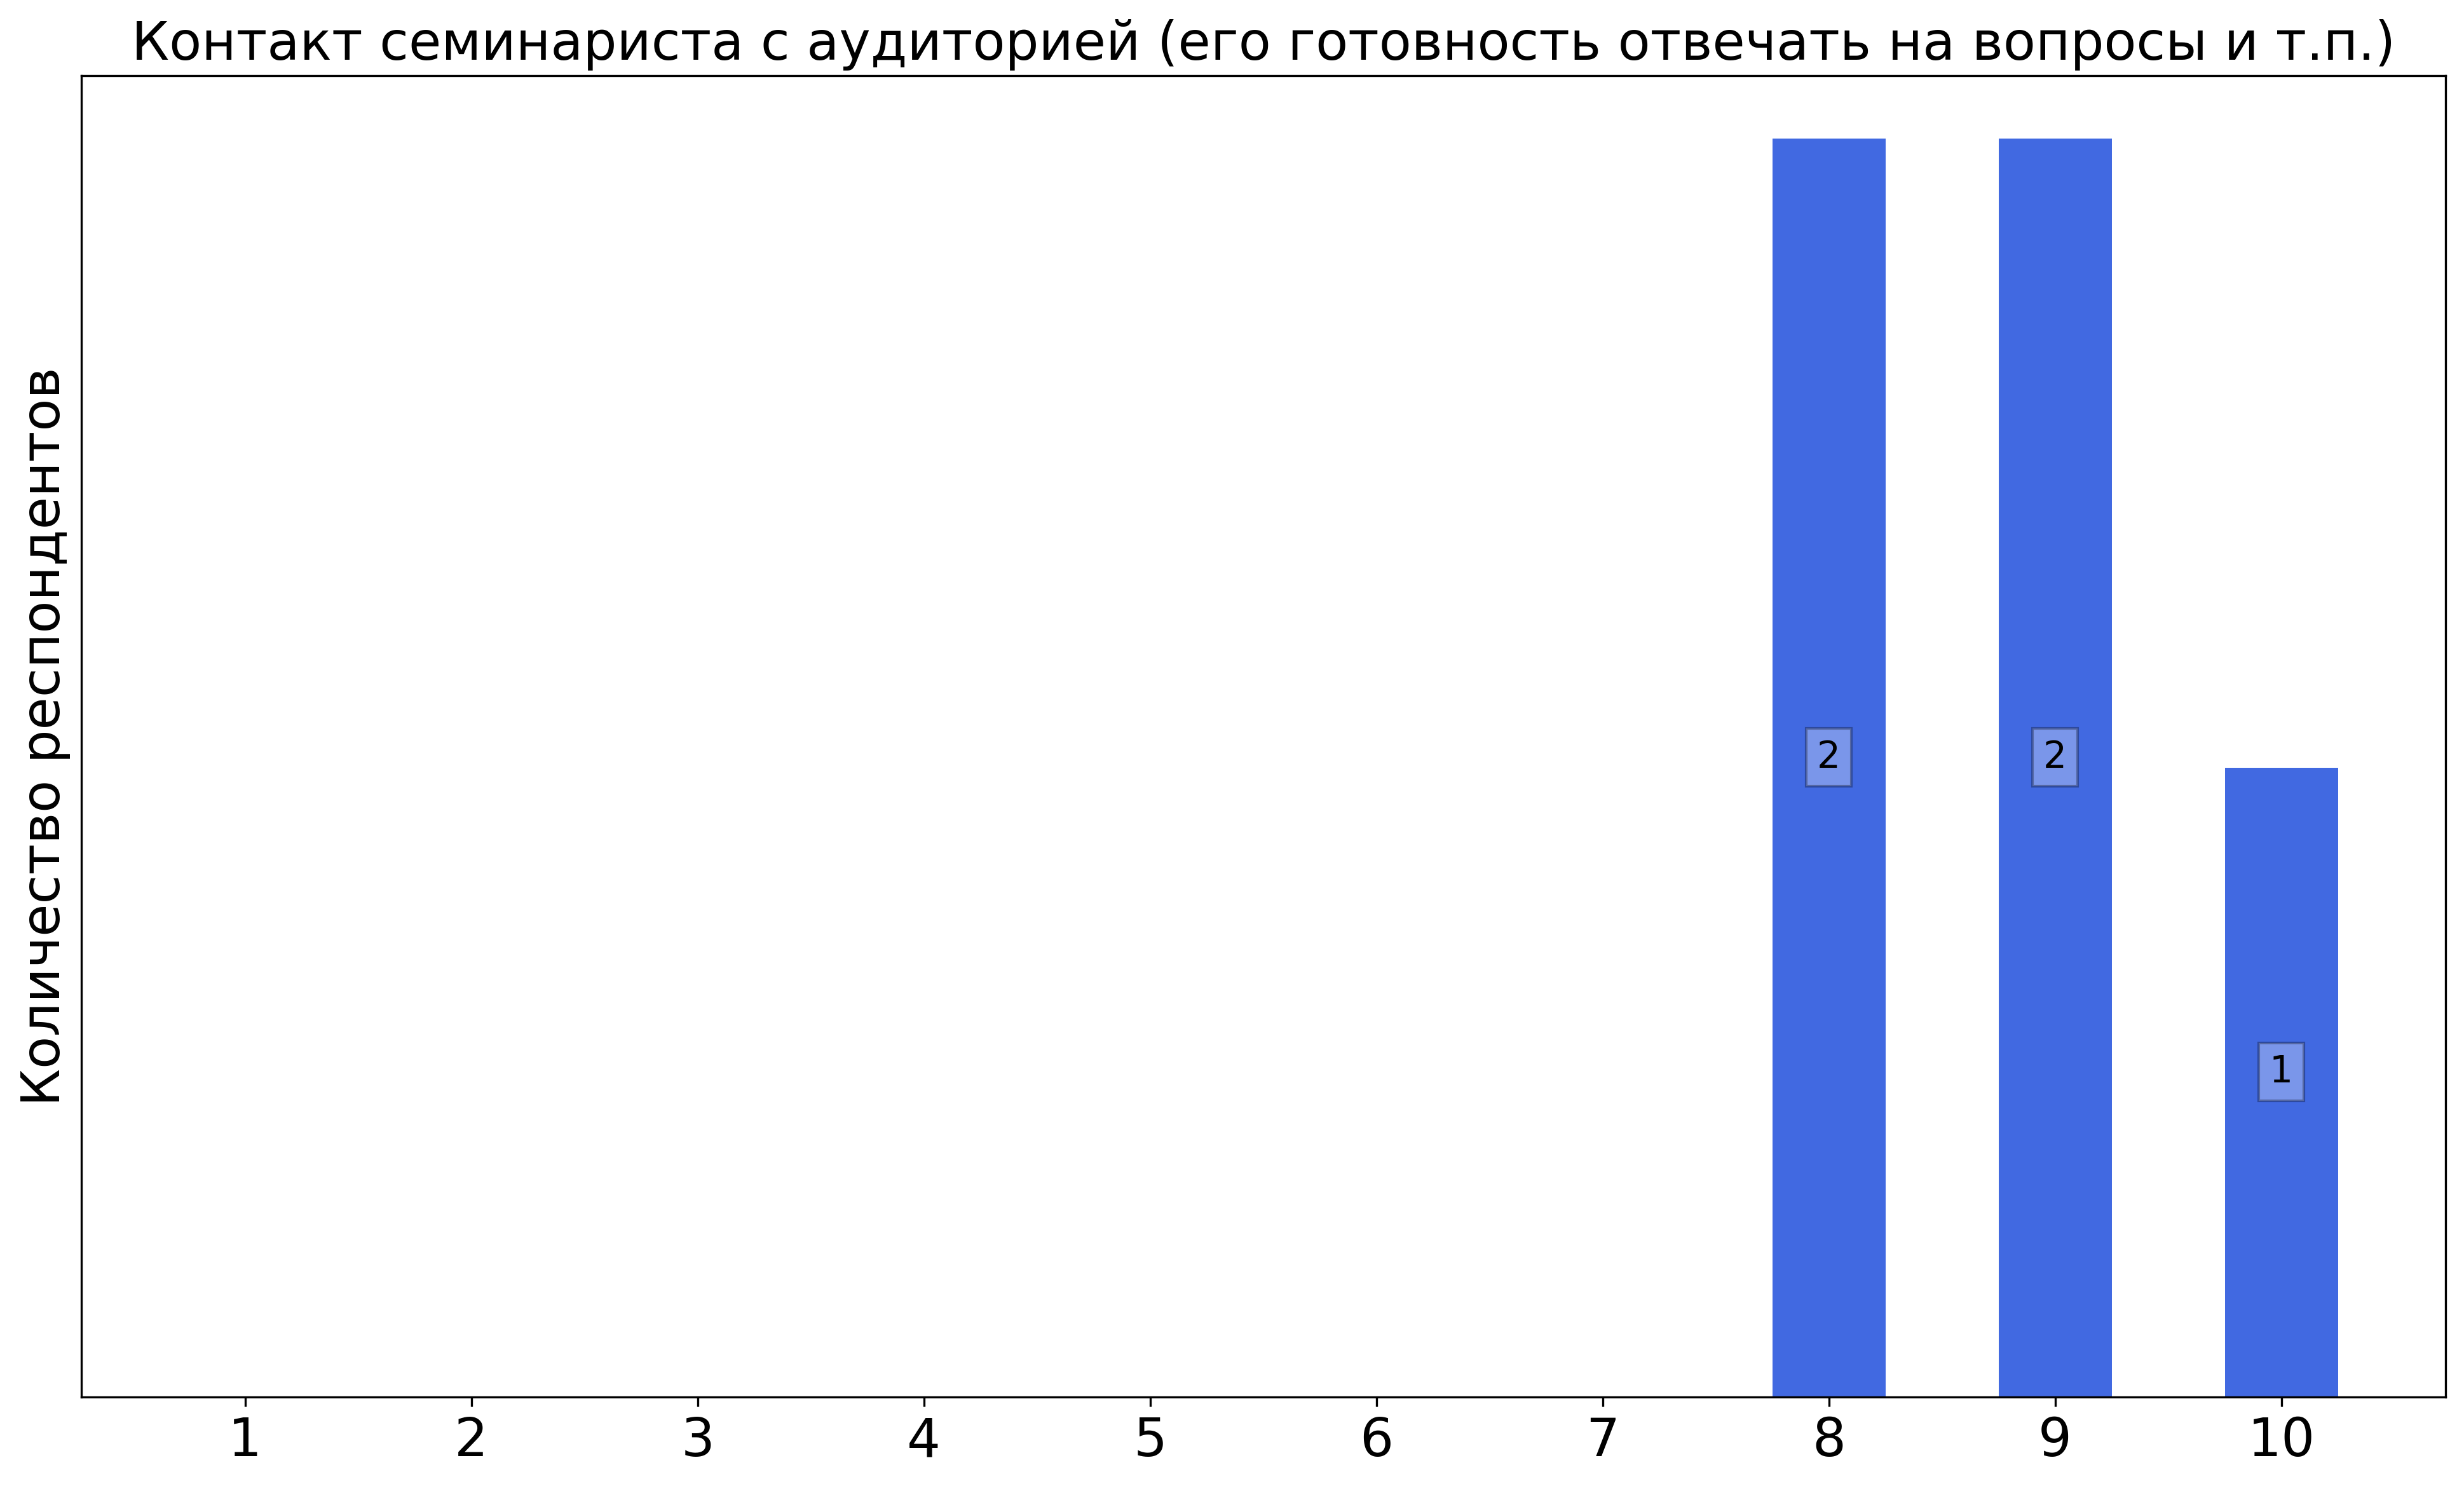
\includegraphics[width=\textwidth]{images/3 course/Общая физика - квантовая физика/seminarists-marks-Виноградов С.В.-0.png}
                \end{subfigure}
                \begin{subfigure}[b]{0.45\textwidth}
                    \centering
                    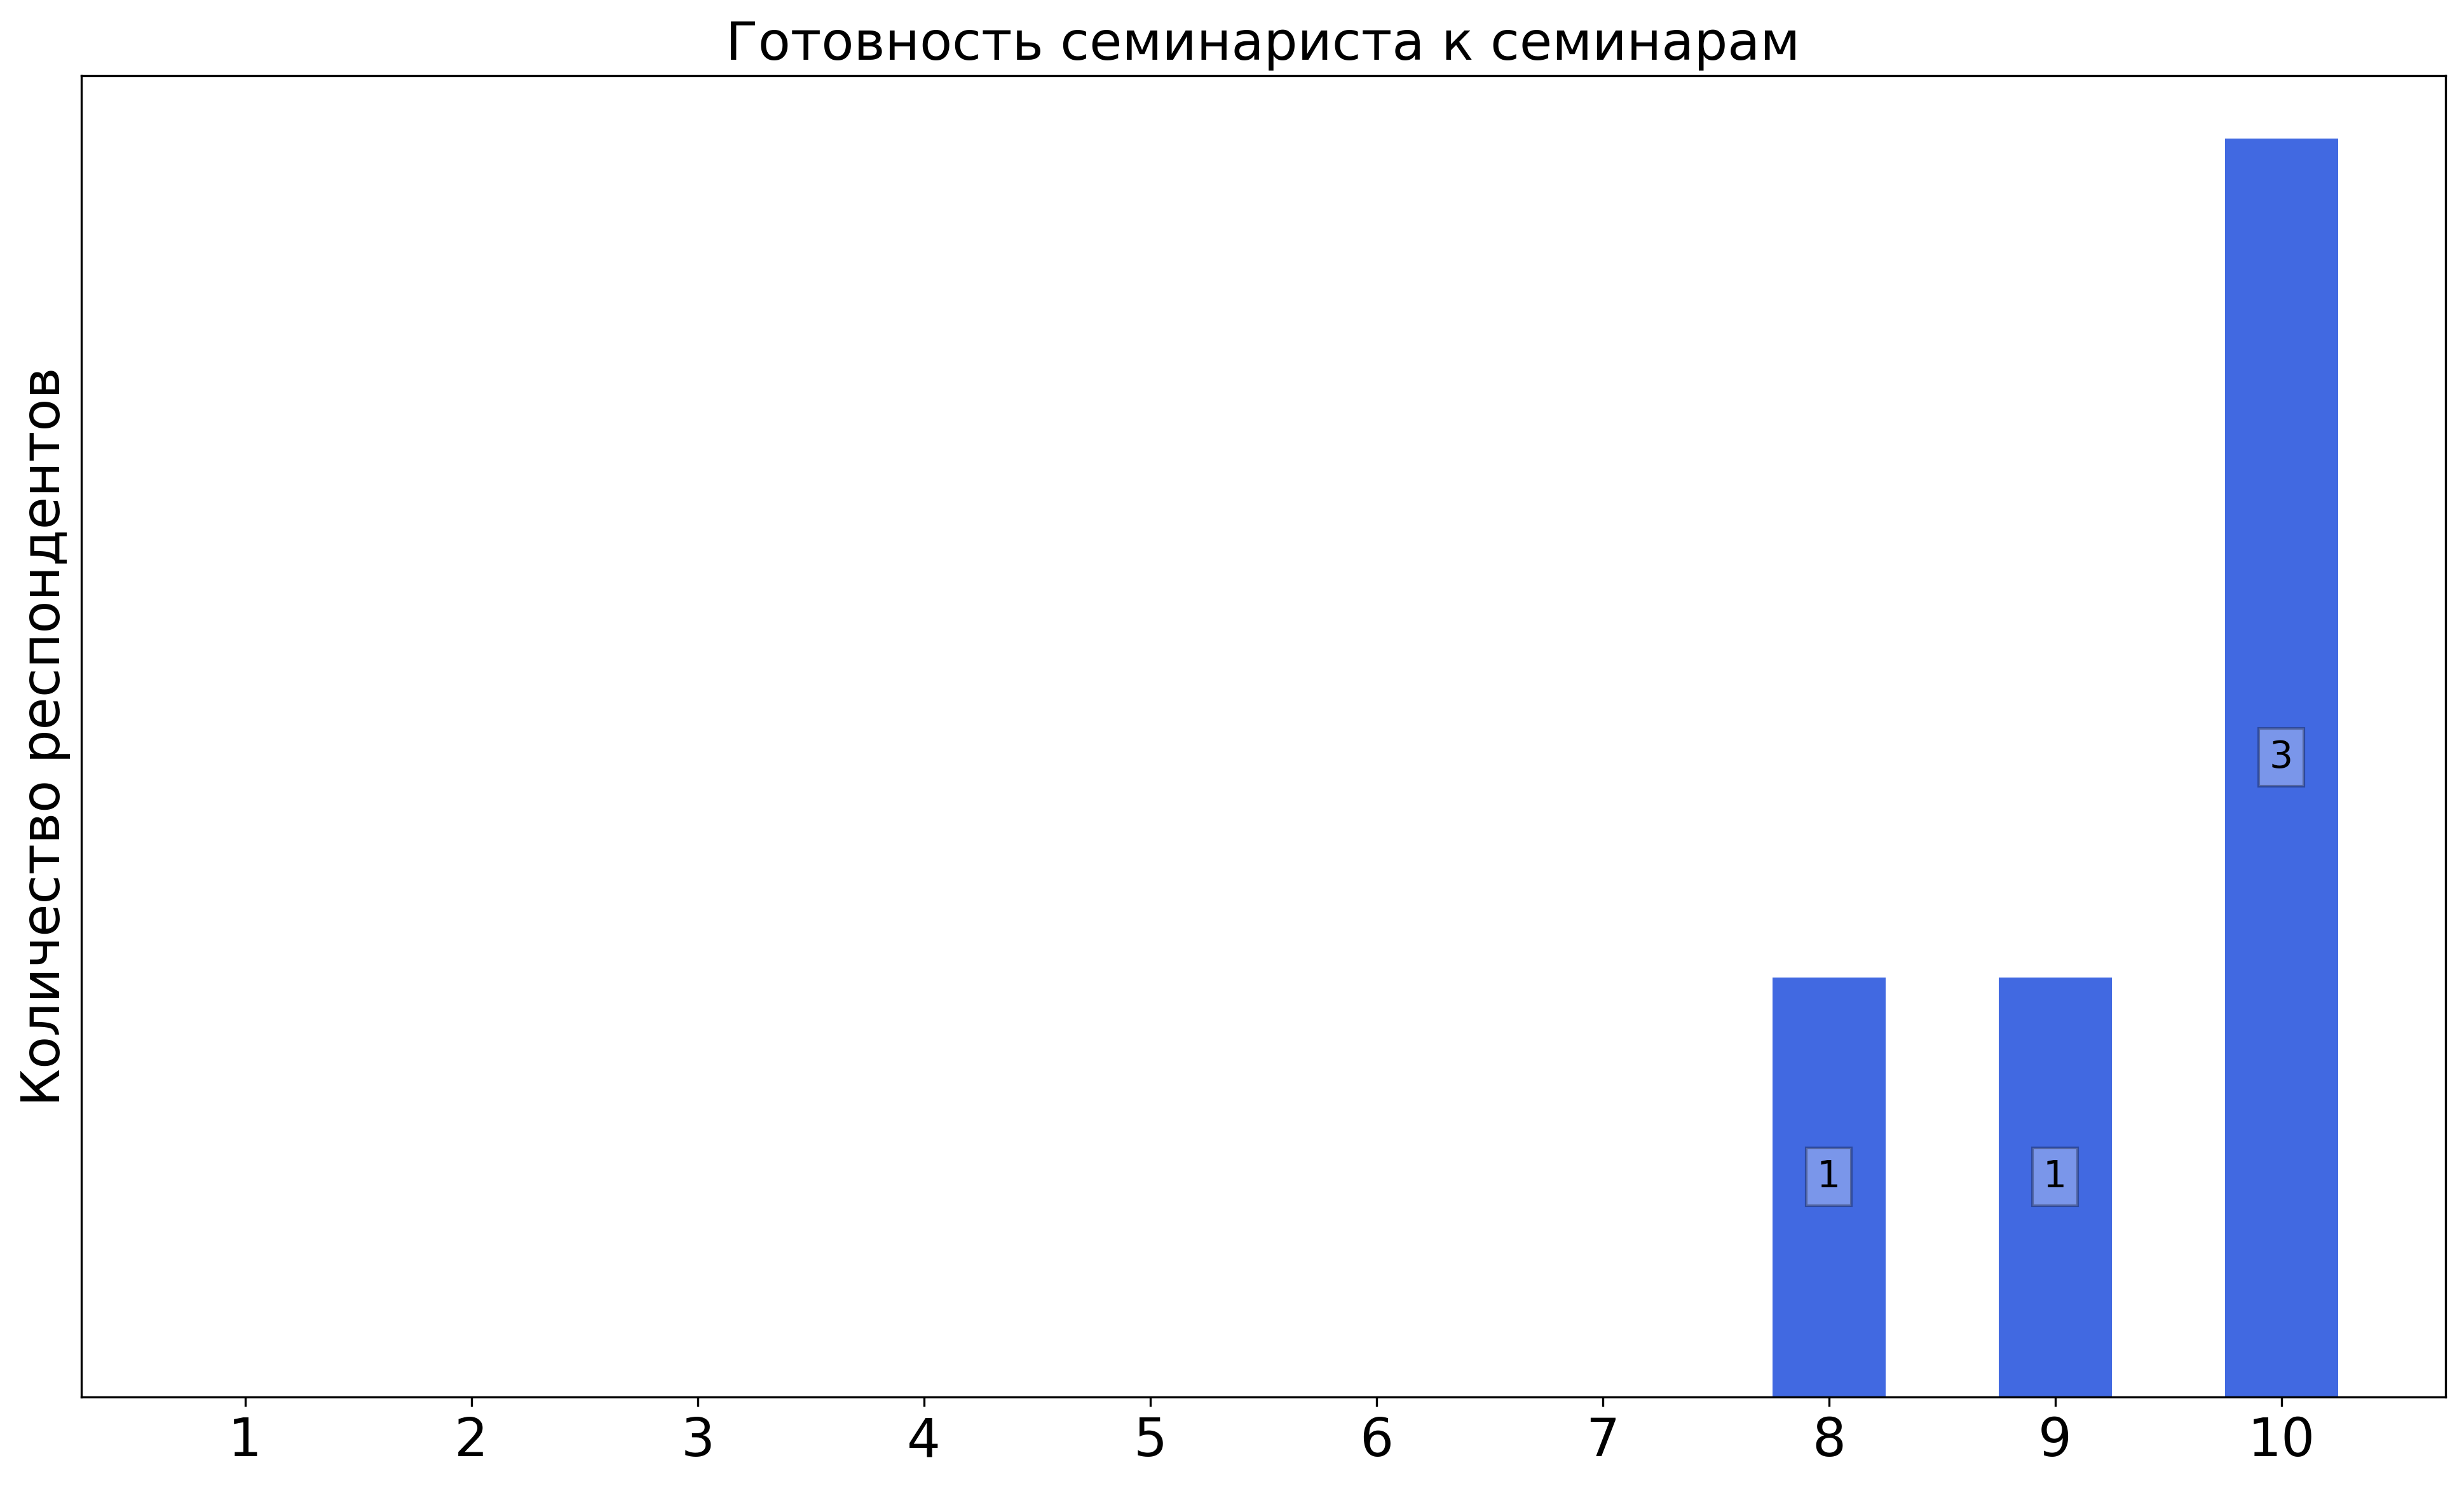
\includegraphics[width=\textwidth]{images/3 course/Общая физика - квантовая физика/seminarists-marks-Виноградов С.В.-1.png}
                \end{subfigure}
                \begin{subfigure}[b]{0.45\textwidth}
                    \centering
                    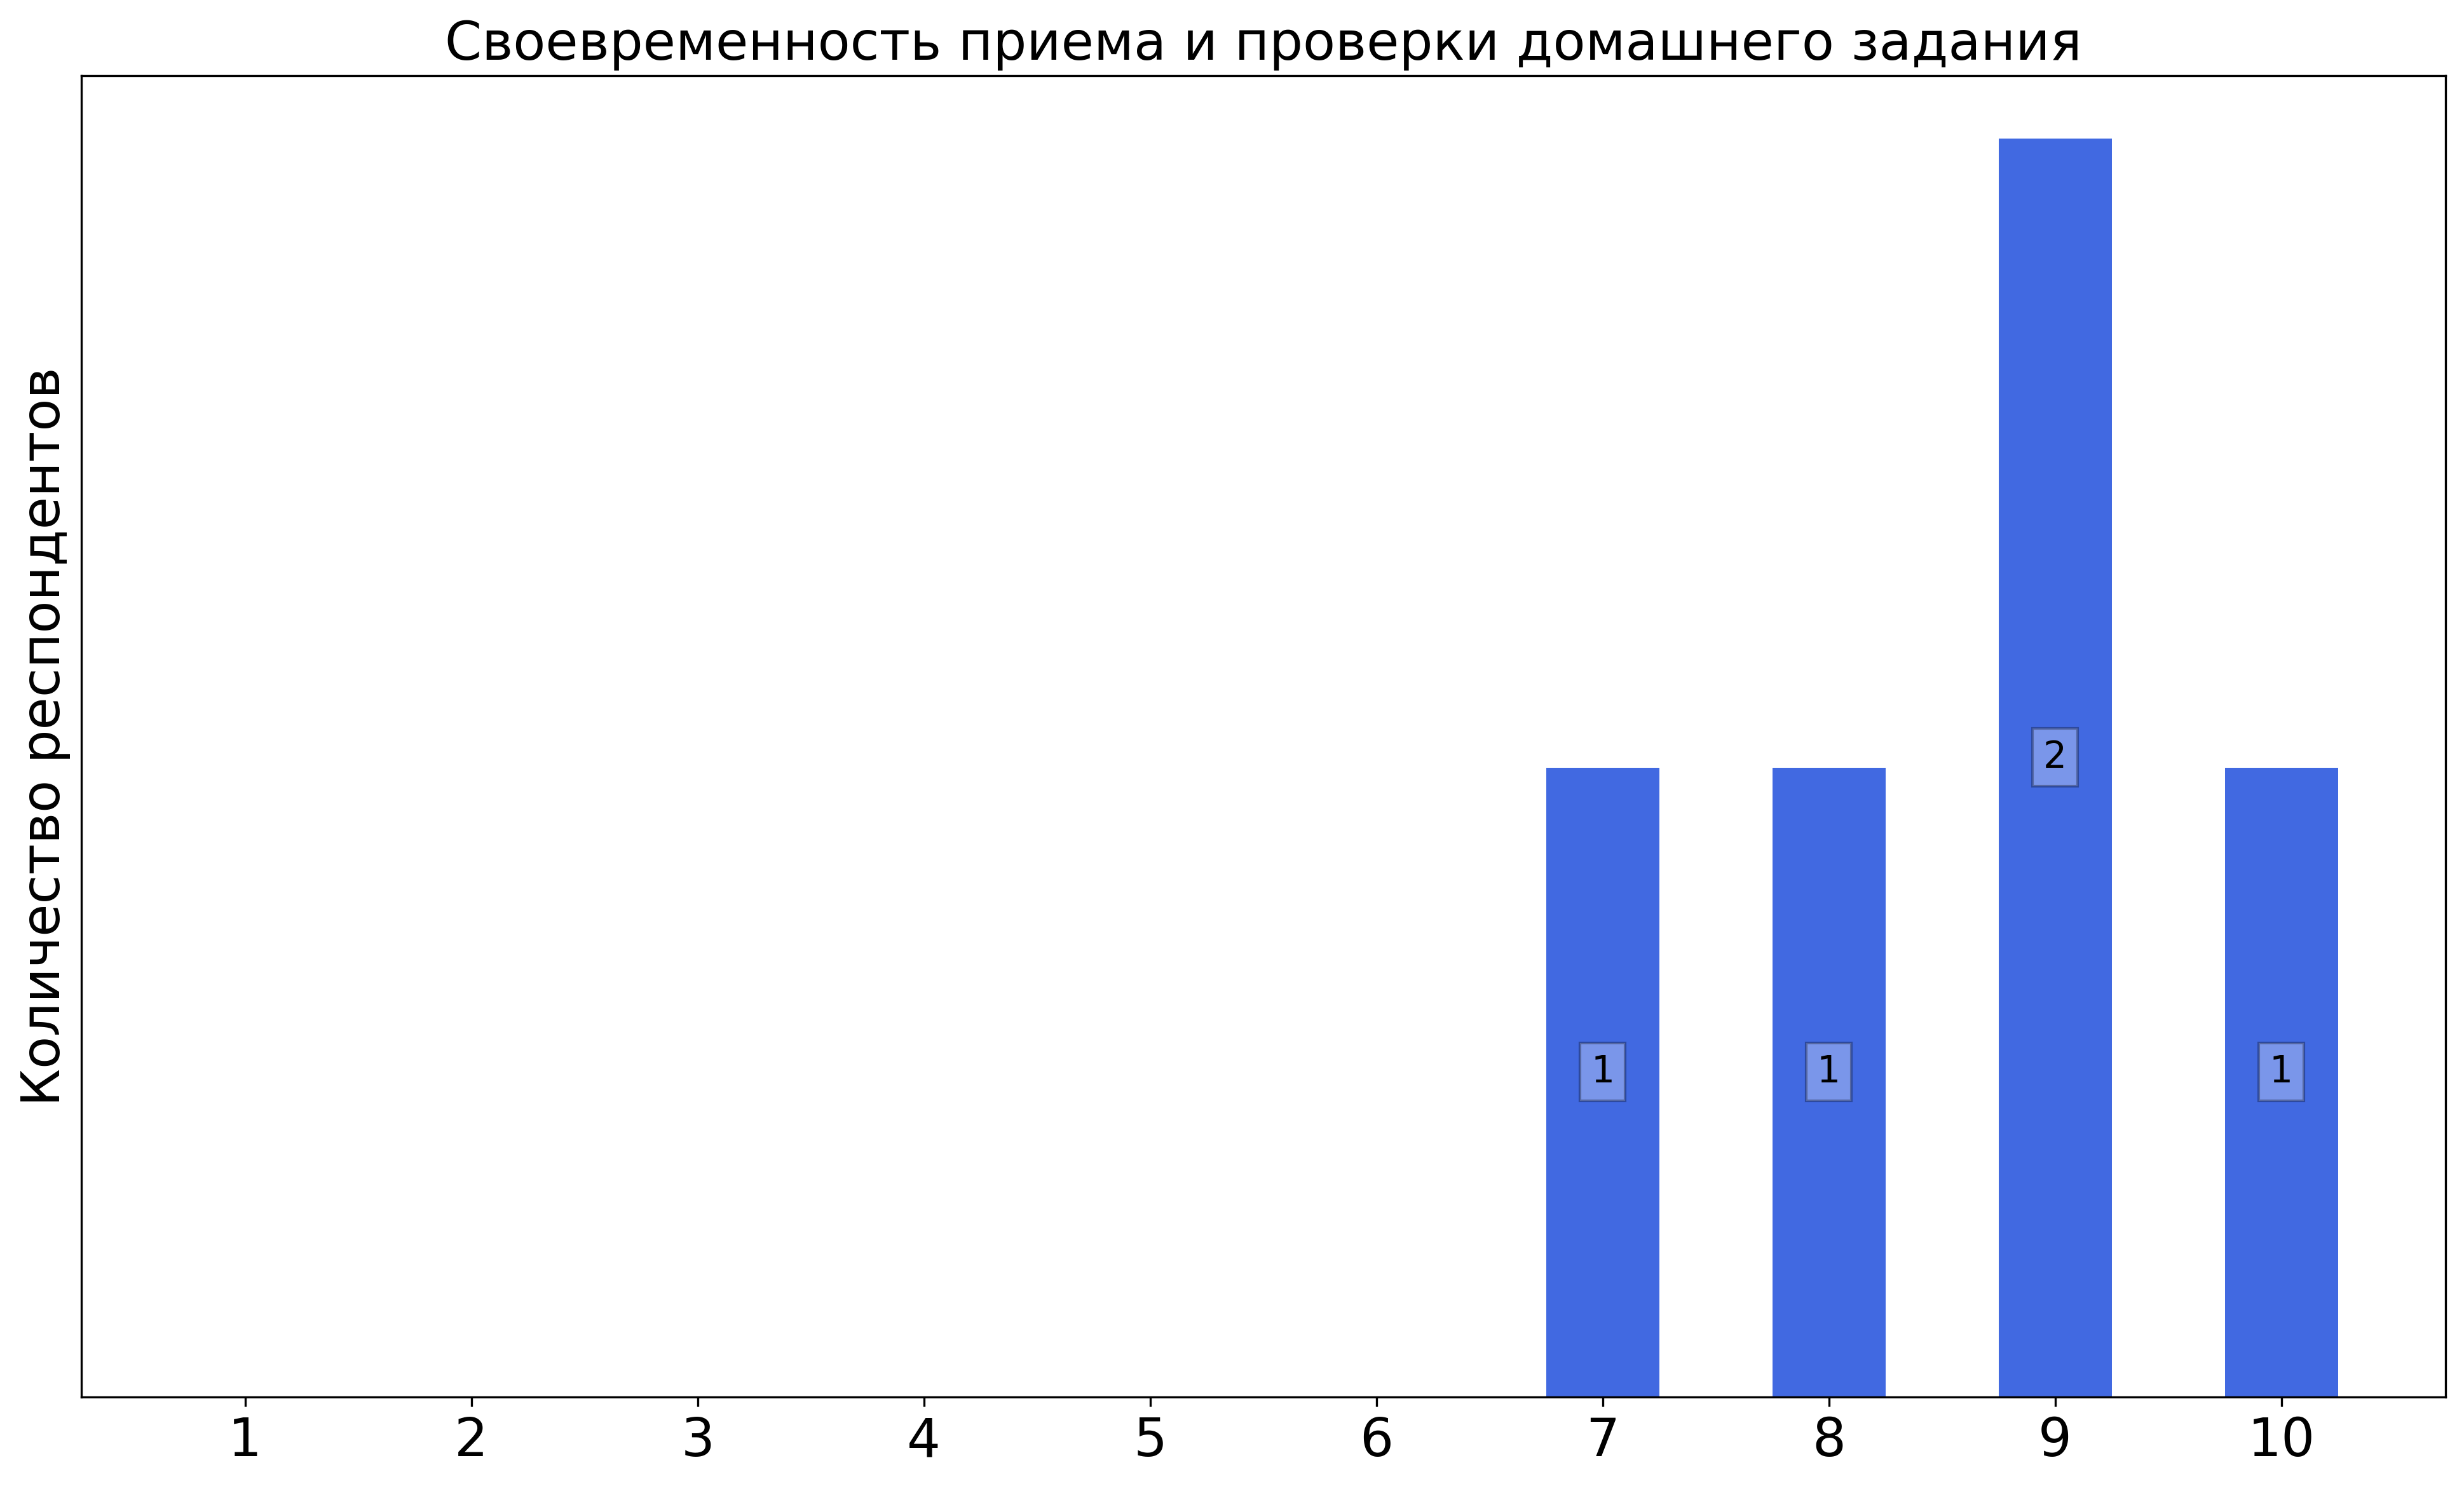
\includegraphics[width=\textwidth]{images/3 course/Общая физика - квантовая физика/seminarists-marks-Виноградов С.В.-2.png}
                \end{subfigure}
                \begin{subfigure}[b]{0.45\textwidth}
                    \centering
                    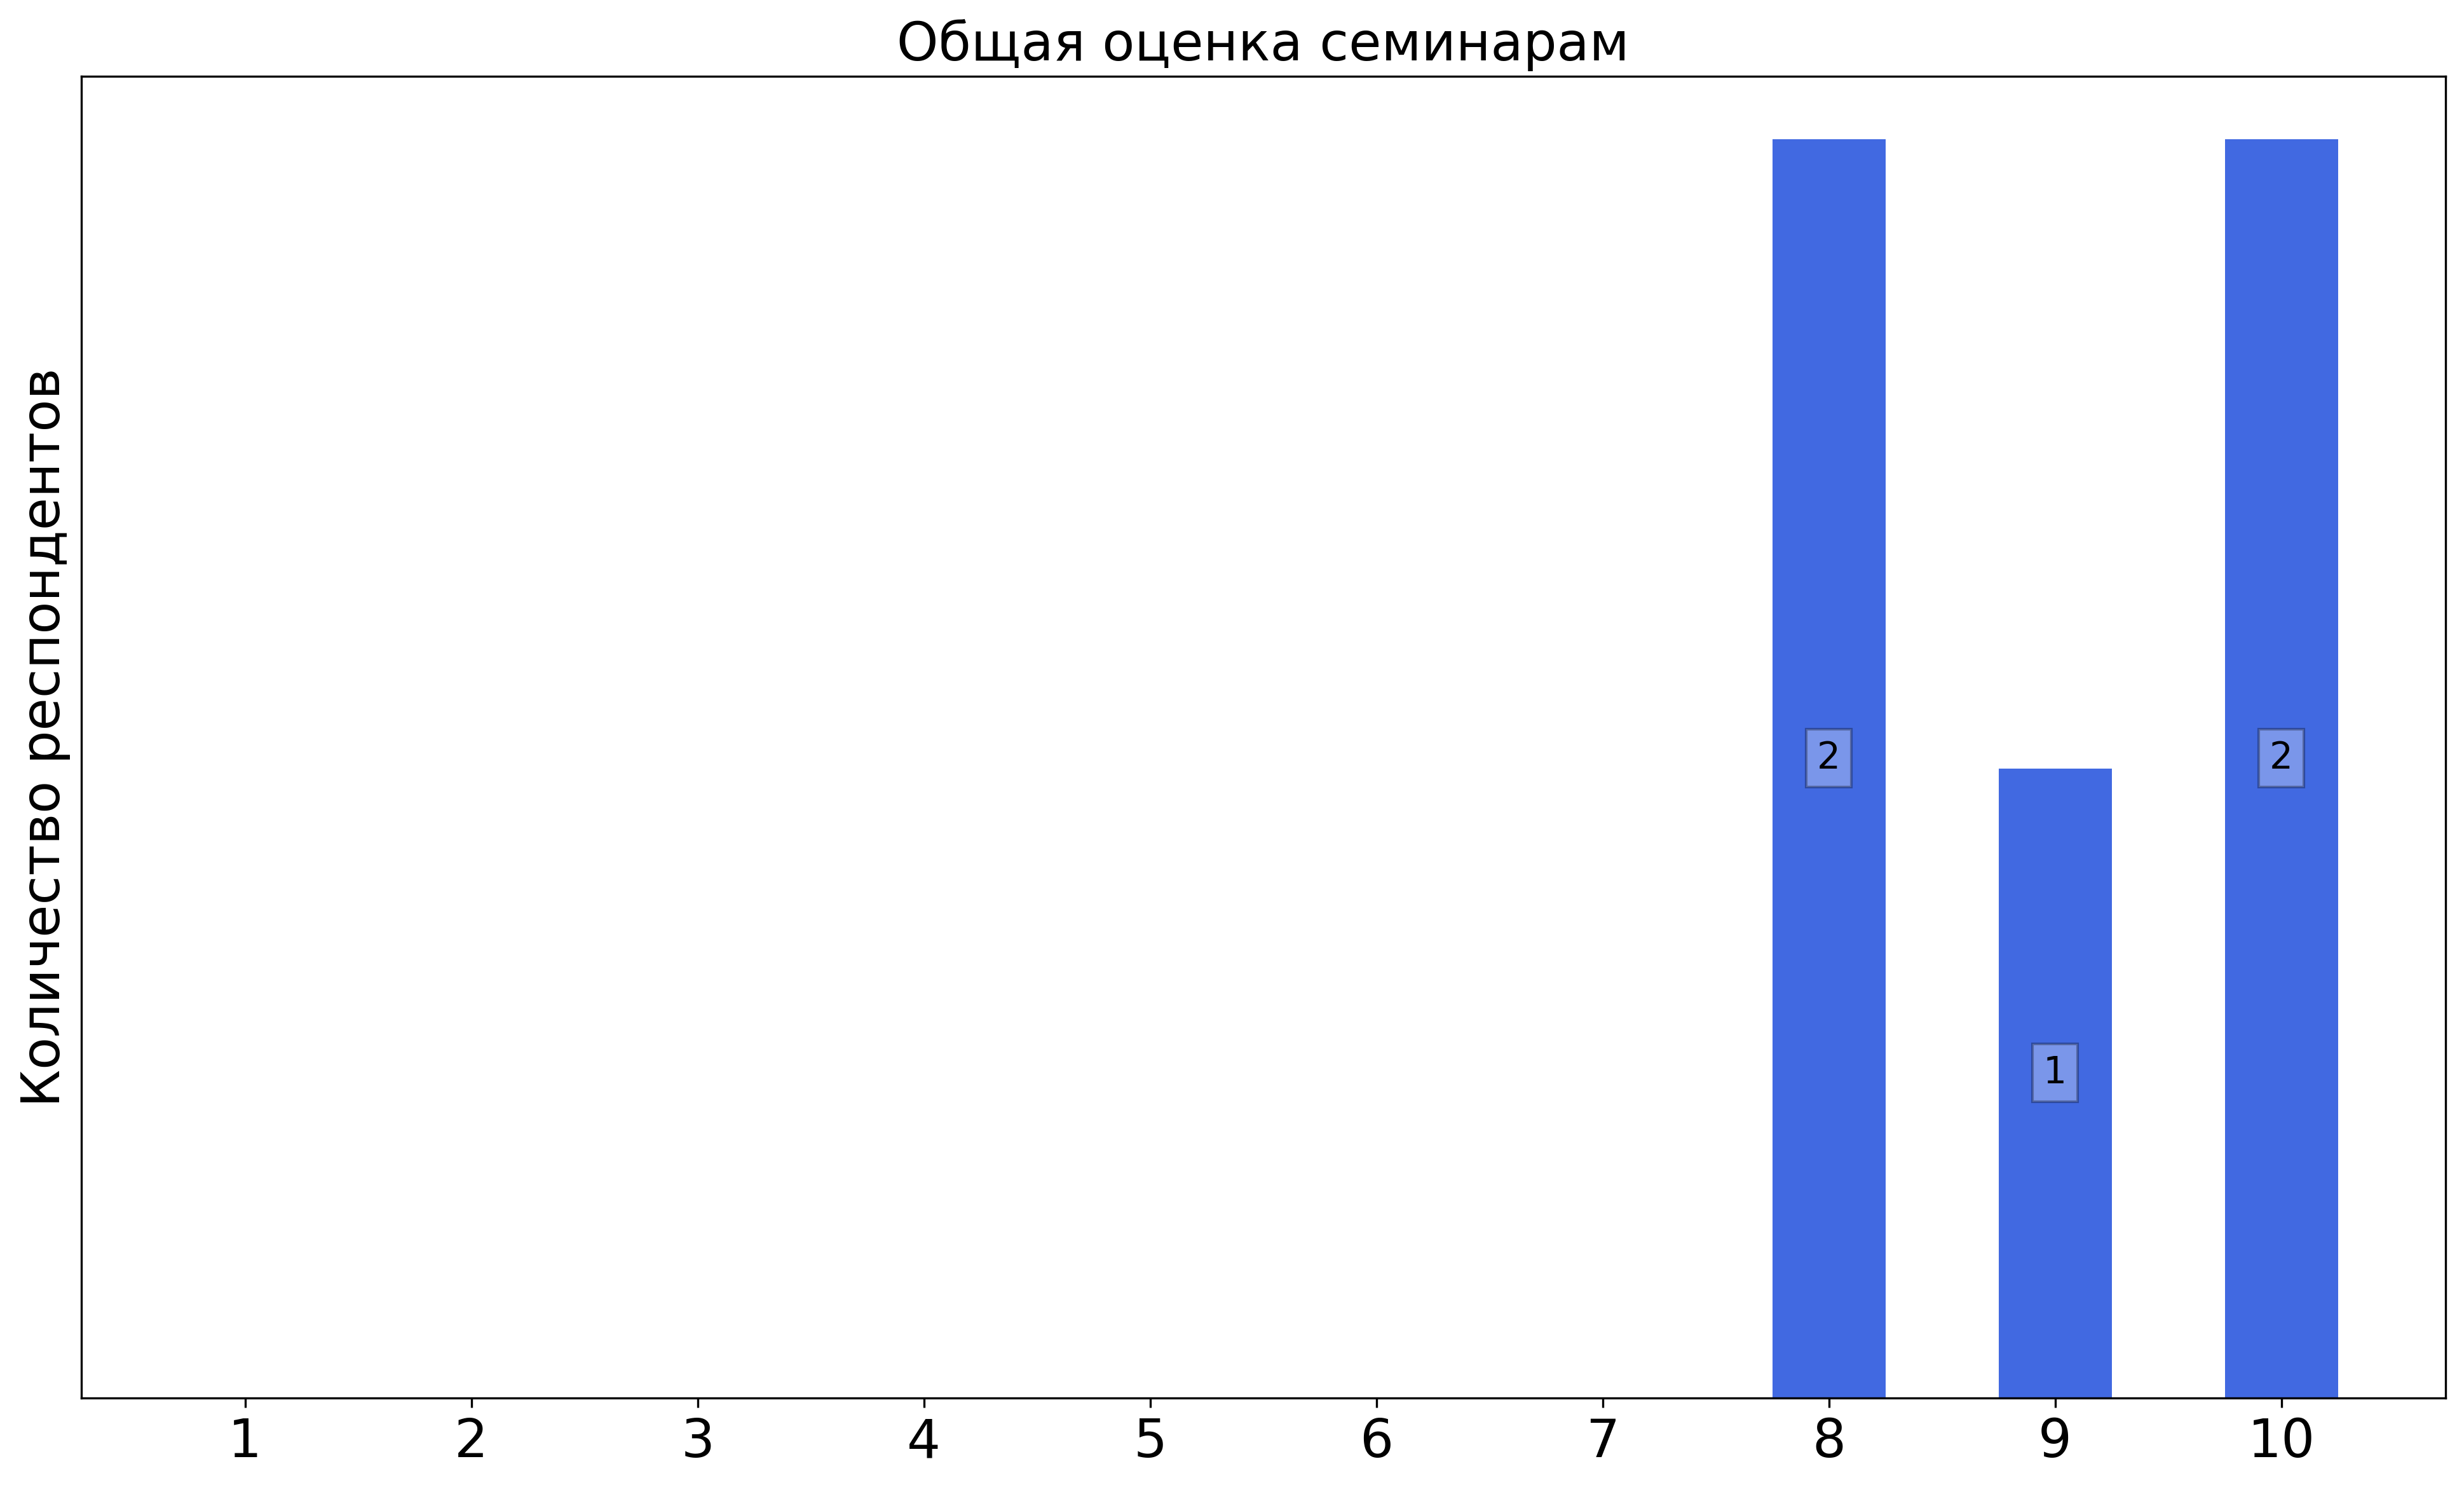
\includegraphics[width=\textwidth]{images/3 course/Общая физика - квантовая физика/seminarists-marks-Виноградов С.В.-3.png}
                \end{subfigure}	
                \caption{Оценки респондентов о качестве преподавания семинаров}
            \end{figure}

            \textbf{Комментарии студентов о семинаристе\protect\footnote{сохранены оригинальные орфография и пунктуация}}
                \begin{commentbox} 
                    Виноградов отличный препод и крутой мужик 
                \end{commentbox} 
            
                \begin{commentbox} 
                    Не всегда понятные обьяснения задач, зато разбор почти всего задания на семинарах
                    Контрольные хорошие, задачи вполне решаемые  
                \end{commentbox} 
            
                \begin{commentbox} 
                    Хороший семинарист, отвечал на все тупые и не только вопросы, оценивал довольно лояльно. Дал возможность сделать хороший впв. 
                \end{commentbox} 



        \subsubsection{Отзыв студентов о семинарах. Семинарист: Инжечик Л.В.}
            \begin{figure}[H]
                \centering
                \begin{subfigure}[b]{0.45\textwidth}
                    \centering
                    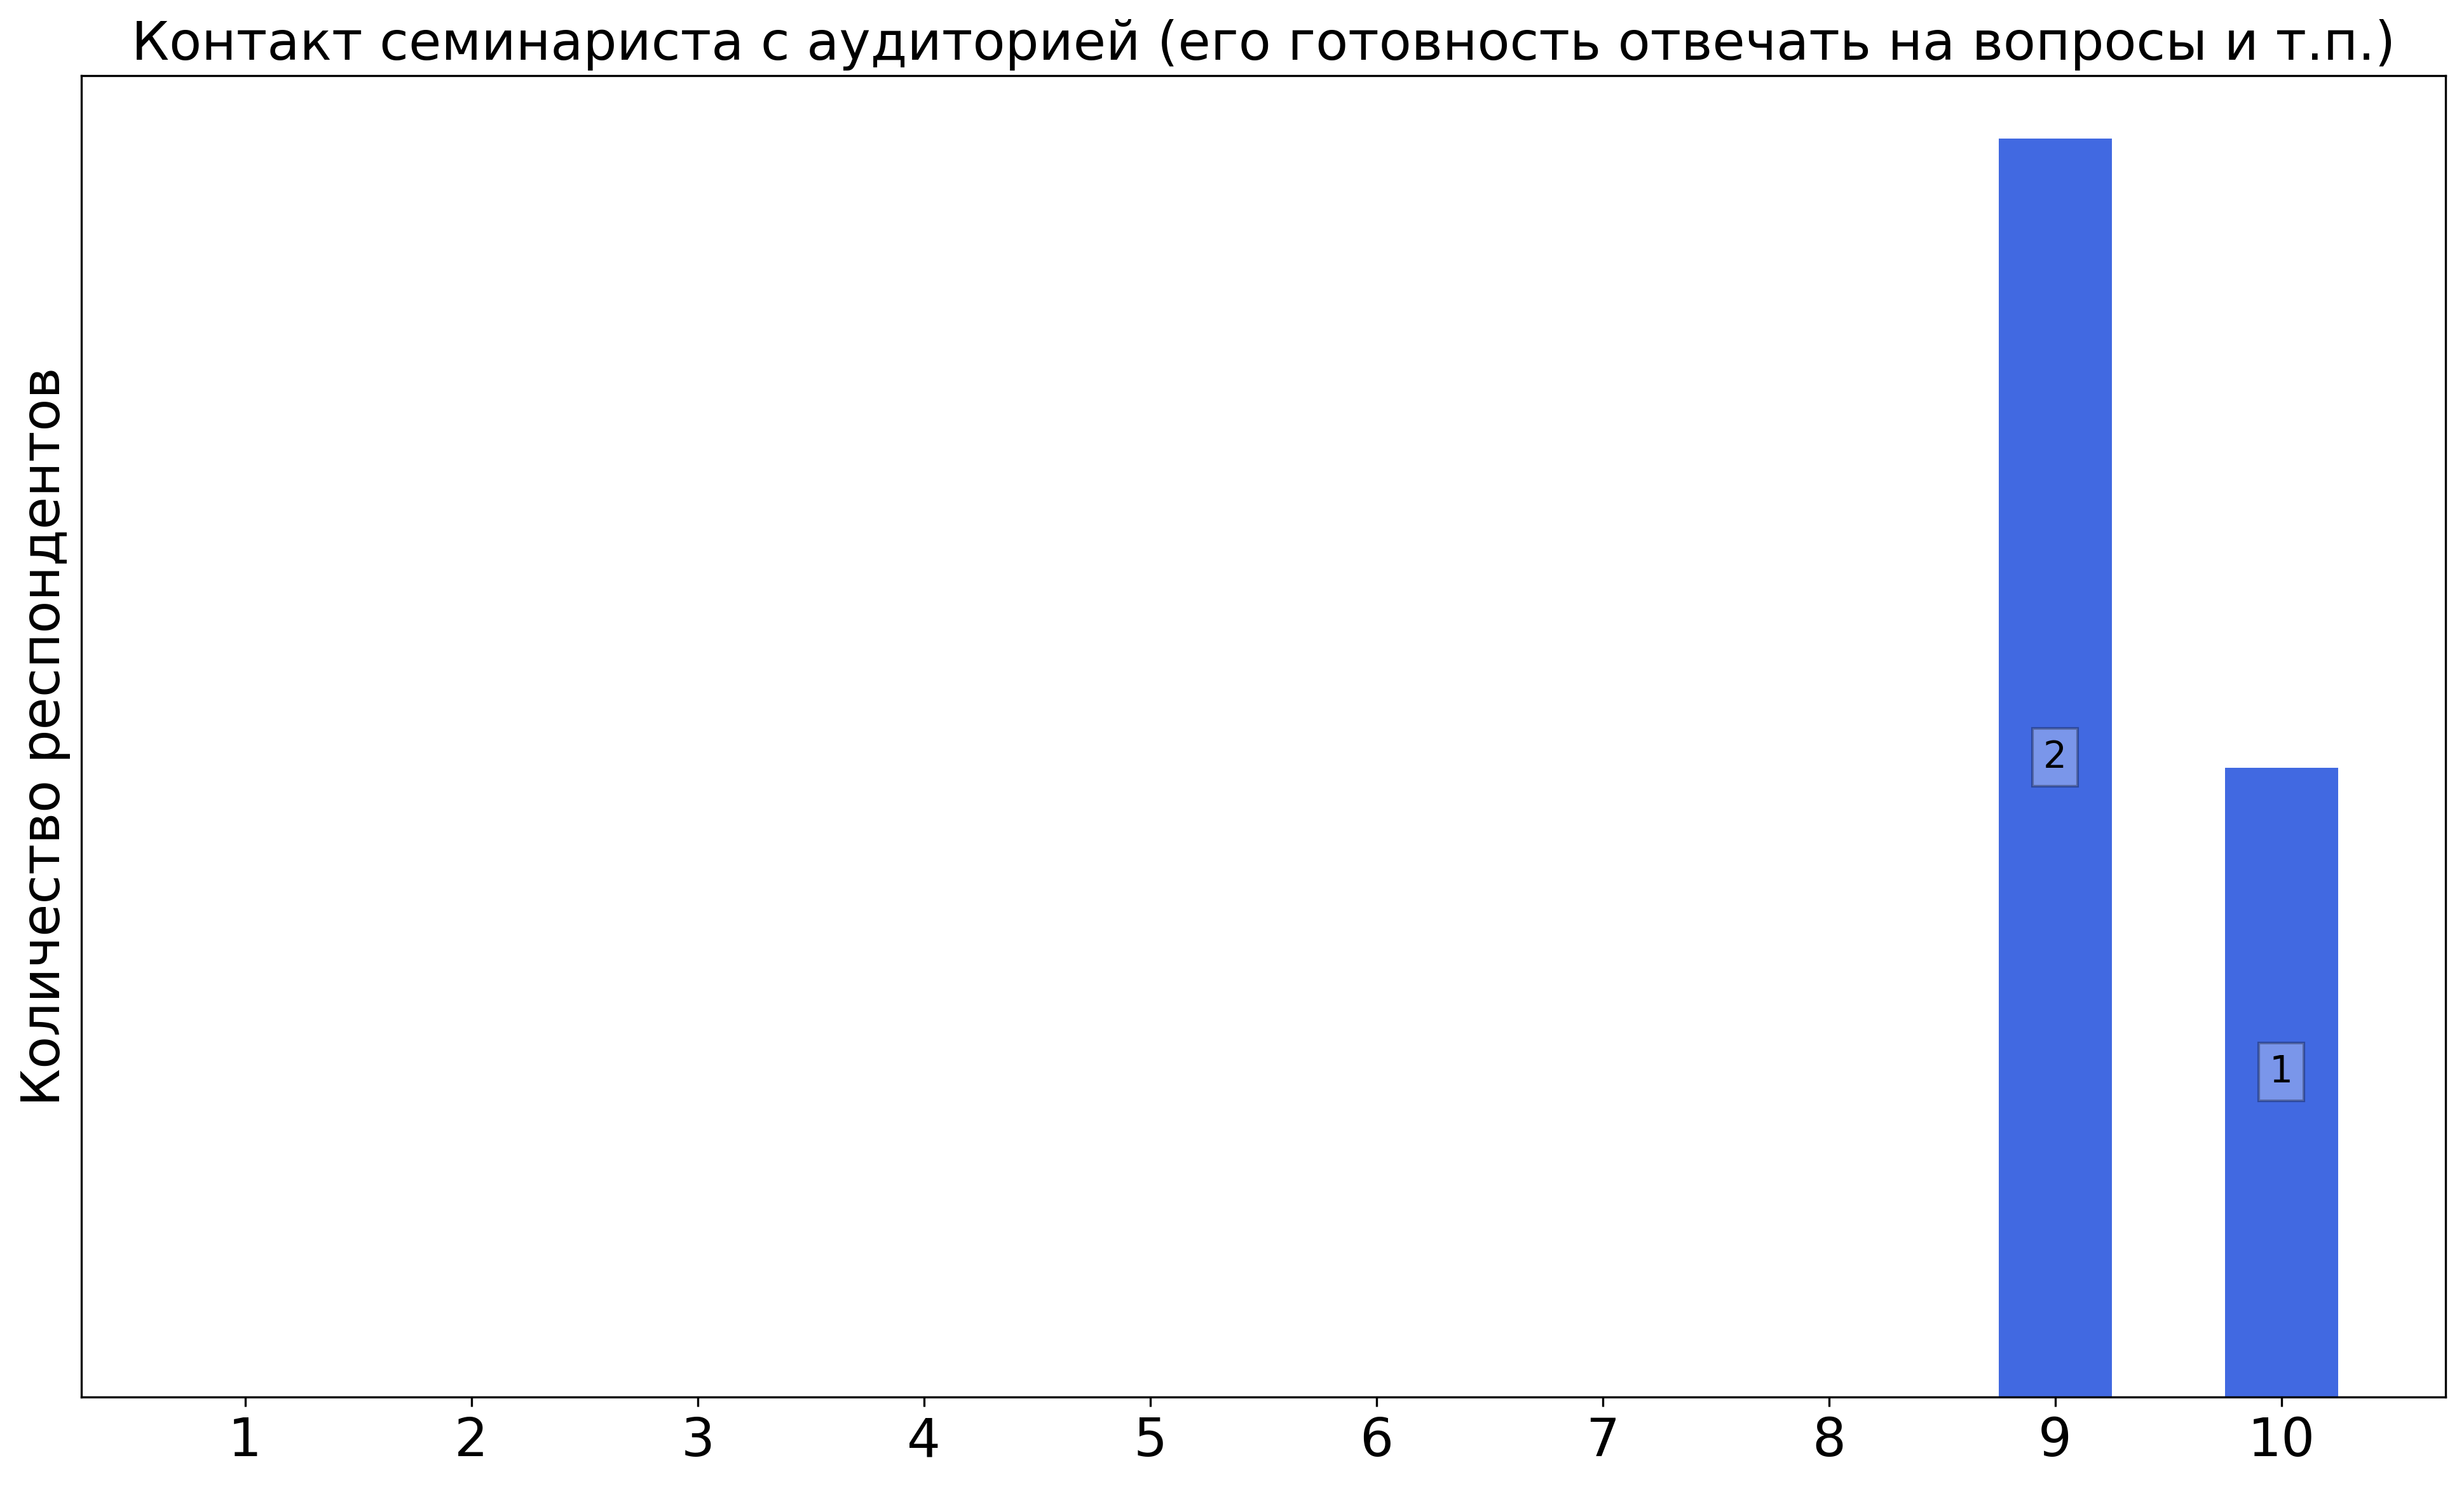
\includegraphics[width=\textwidth]{images/3 course/Общая физика - квантовая физика/seminarists-marks-Инжечик Л.В.-0.png}
                \end{subfigure}
                \begin{subfigure}[b]{0.45\textwidth}
                    \centering
                    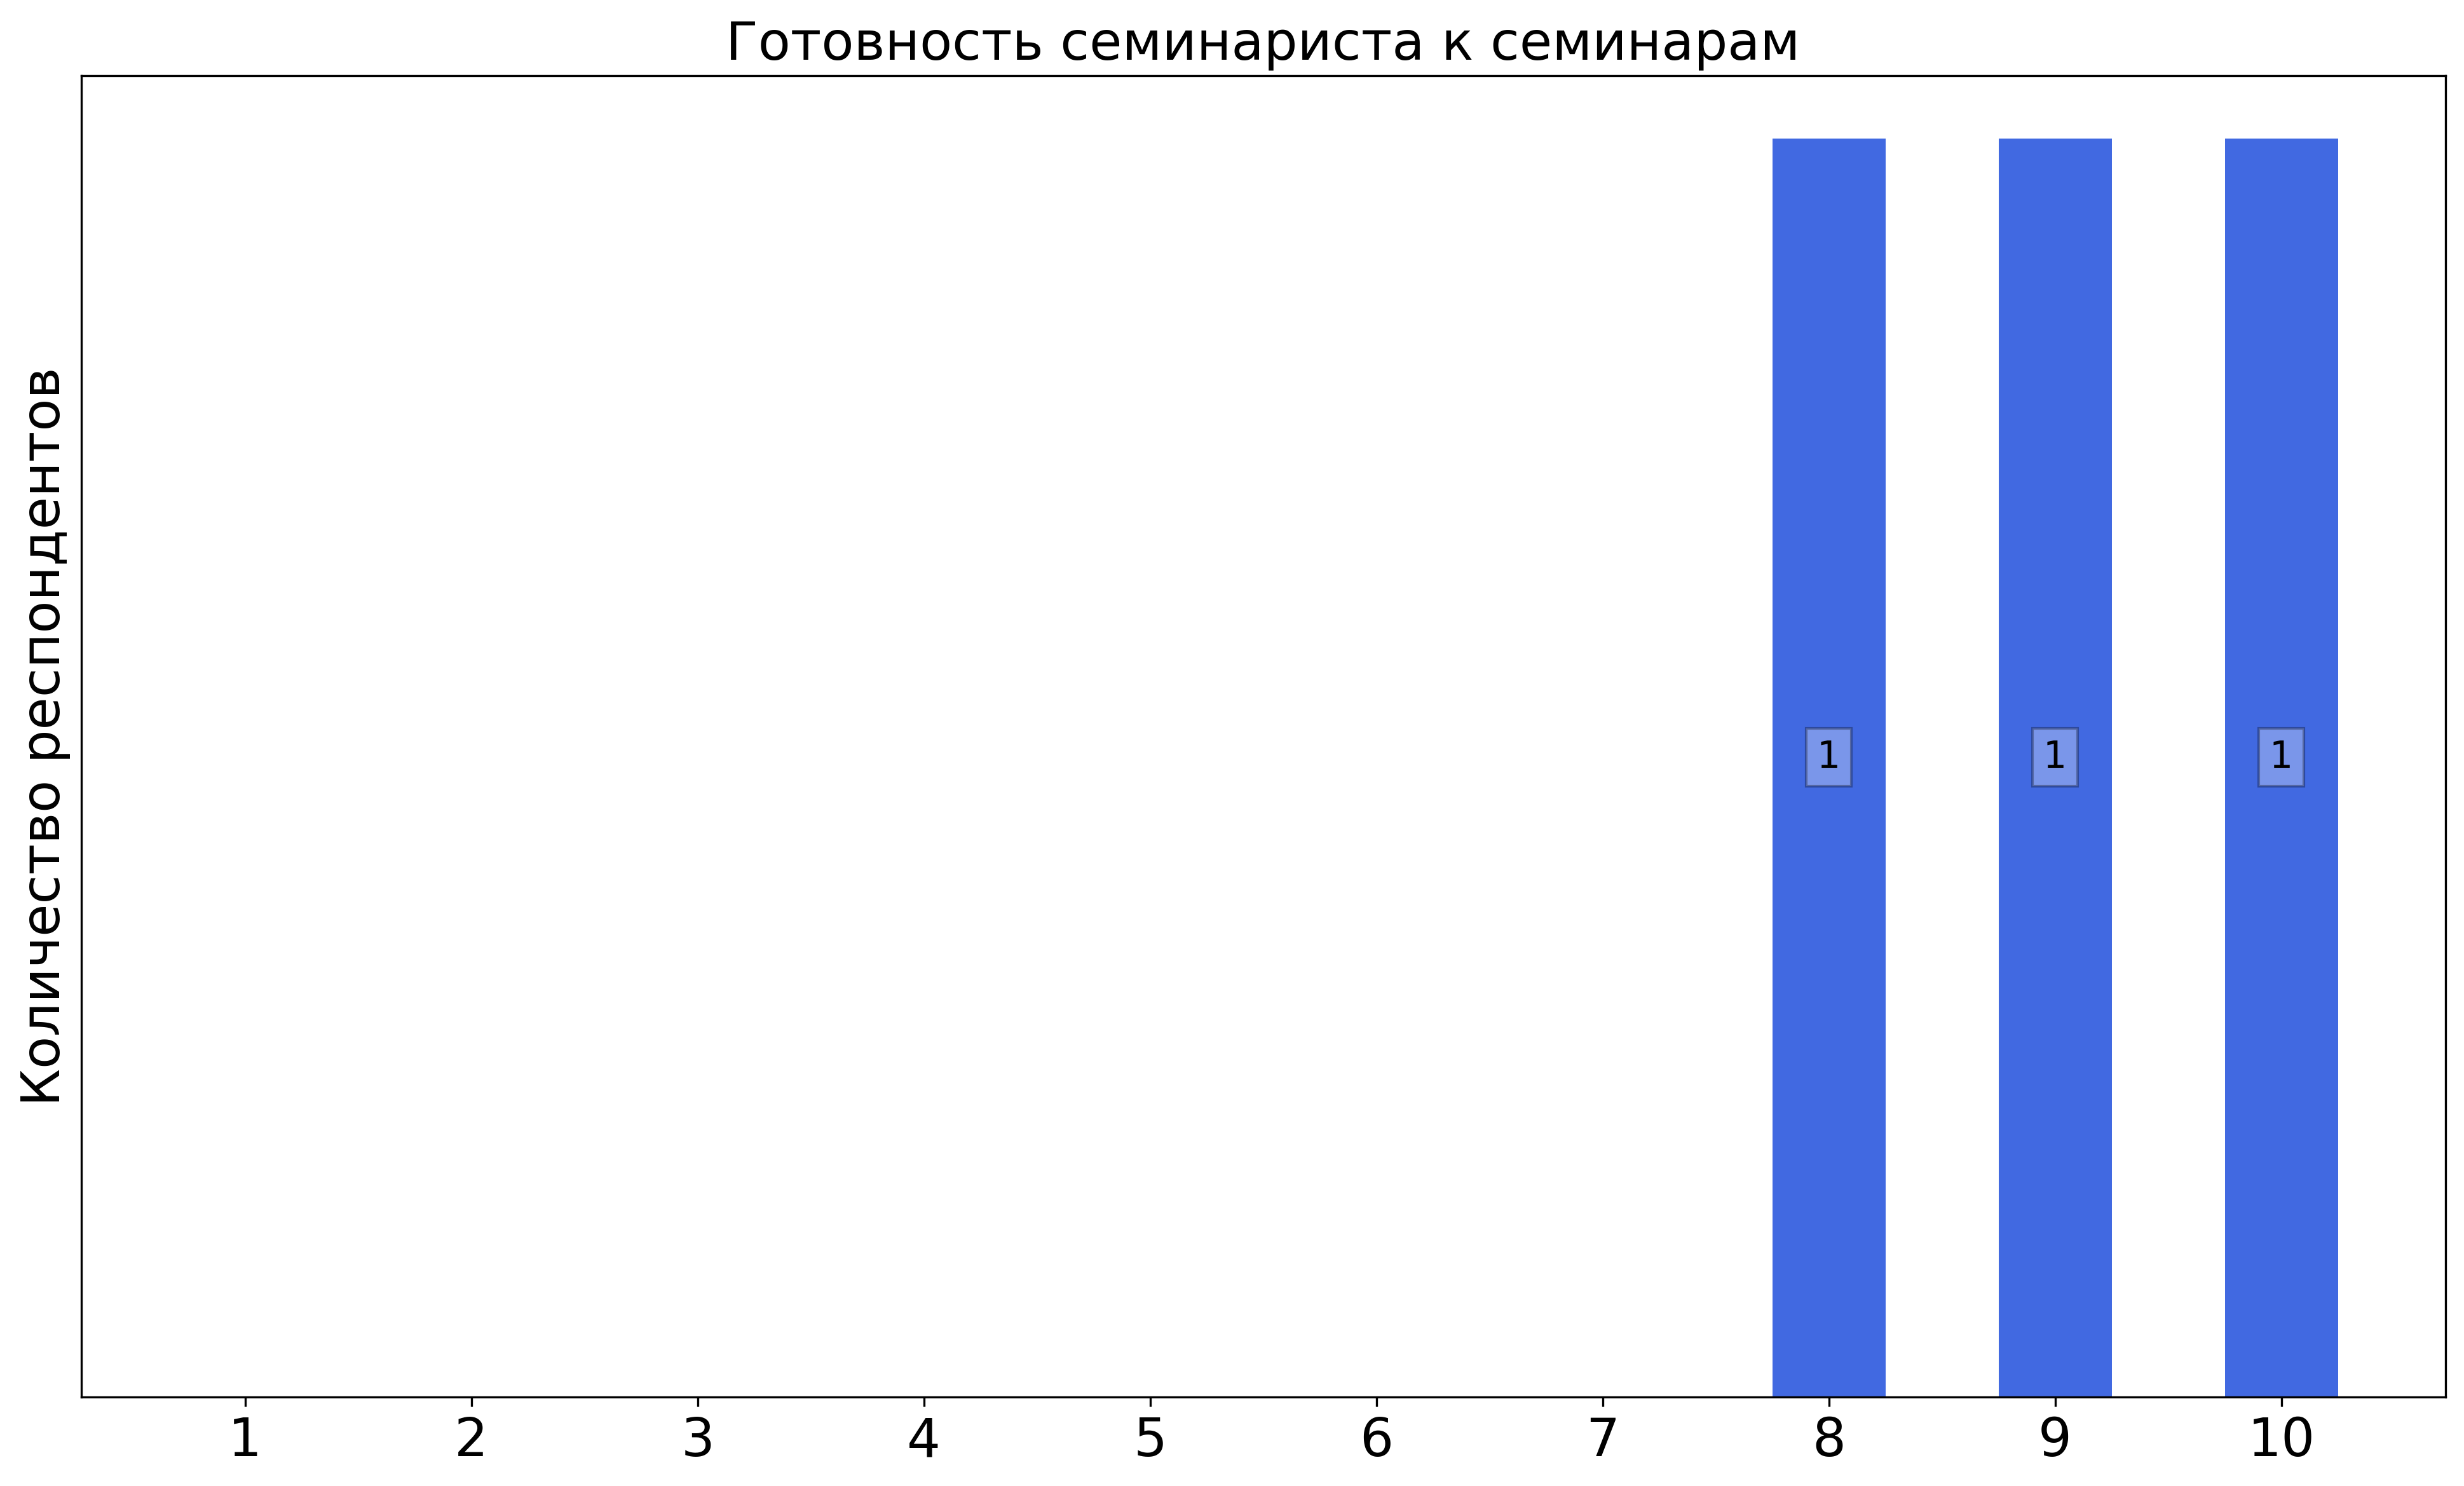
\includegraphics[width=\textwidth]{images/3 course/Общая физика - квантовая физика/seminarists-marks-Инжечик Л.В.-1.png}
                \end{subfigure}
                \begin{subfigure}[b]{0.45\textwidth}
                    \centering
                    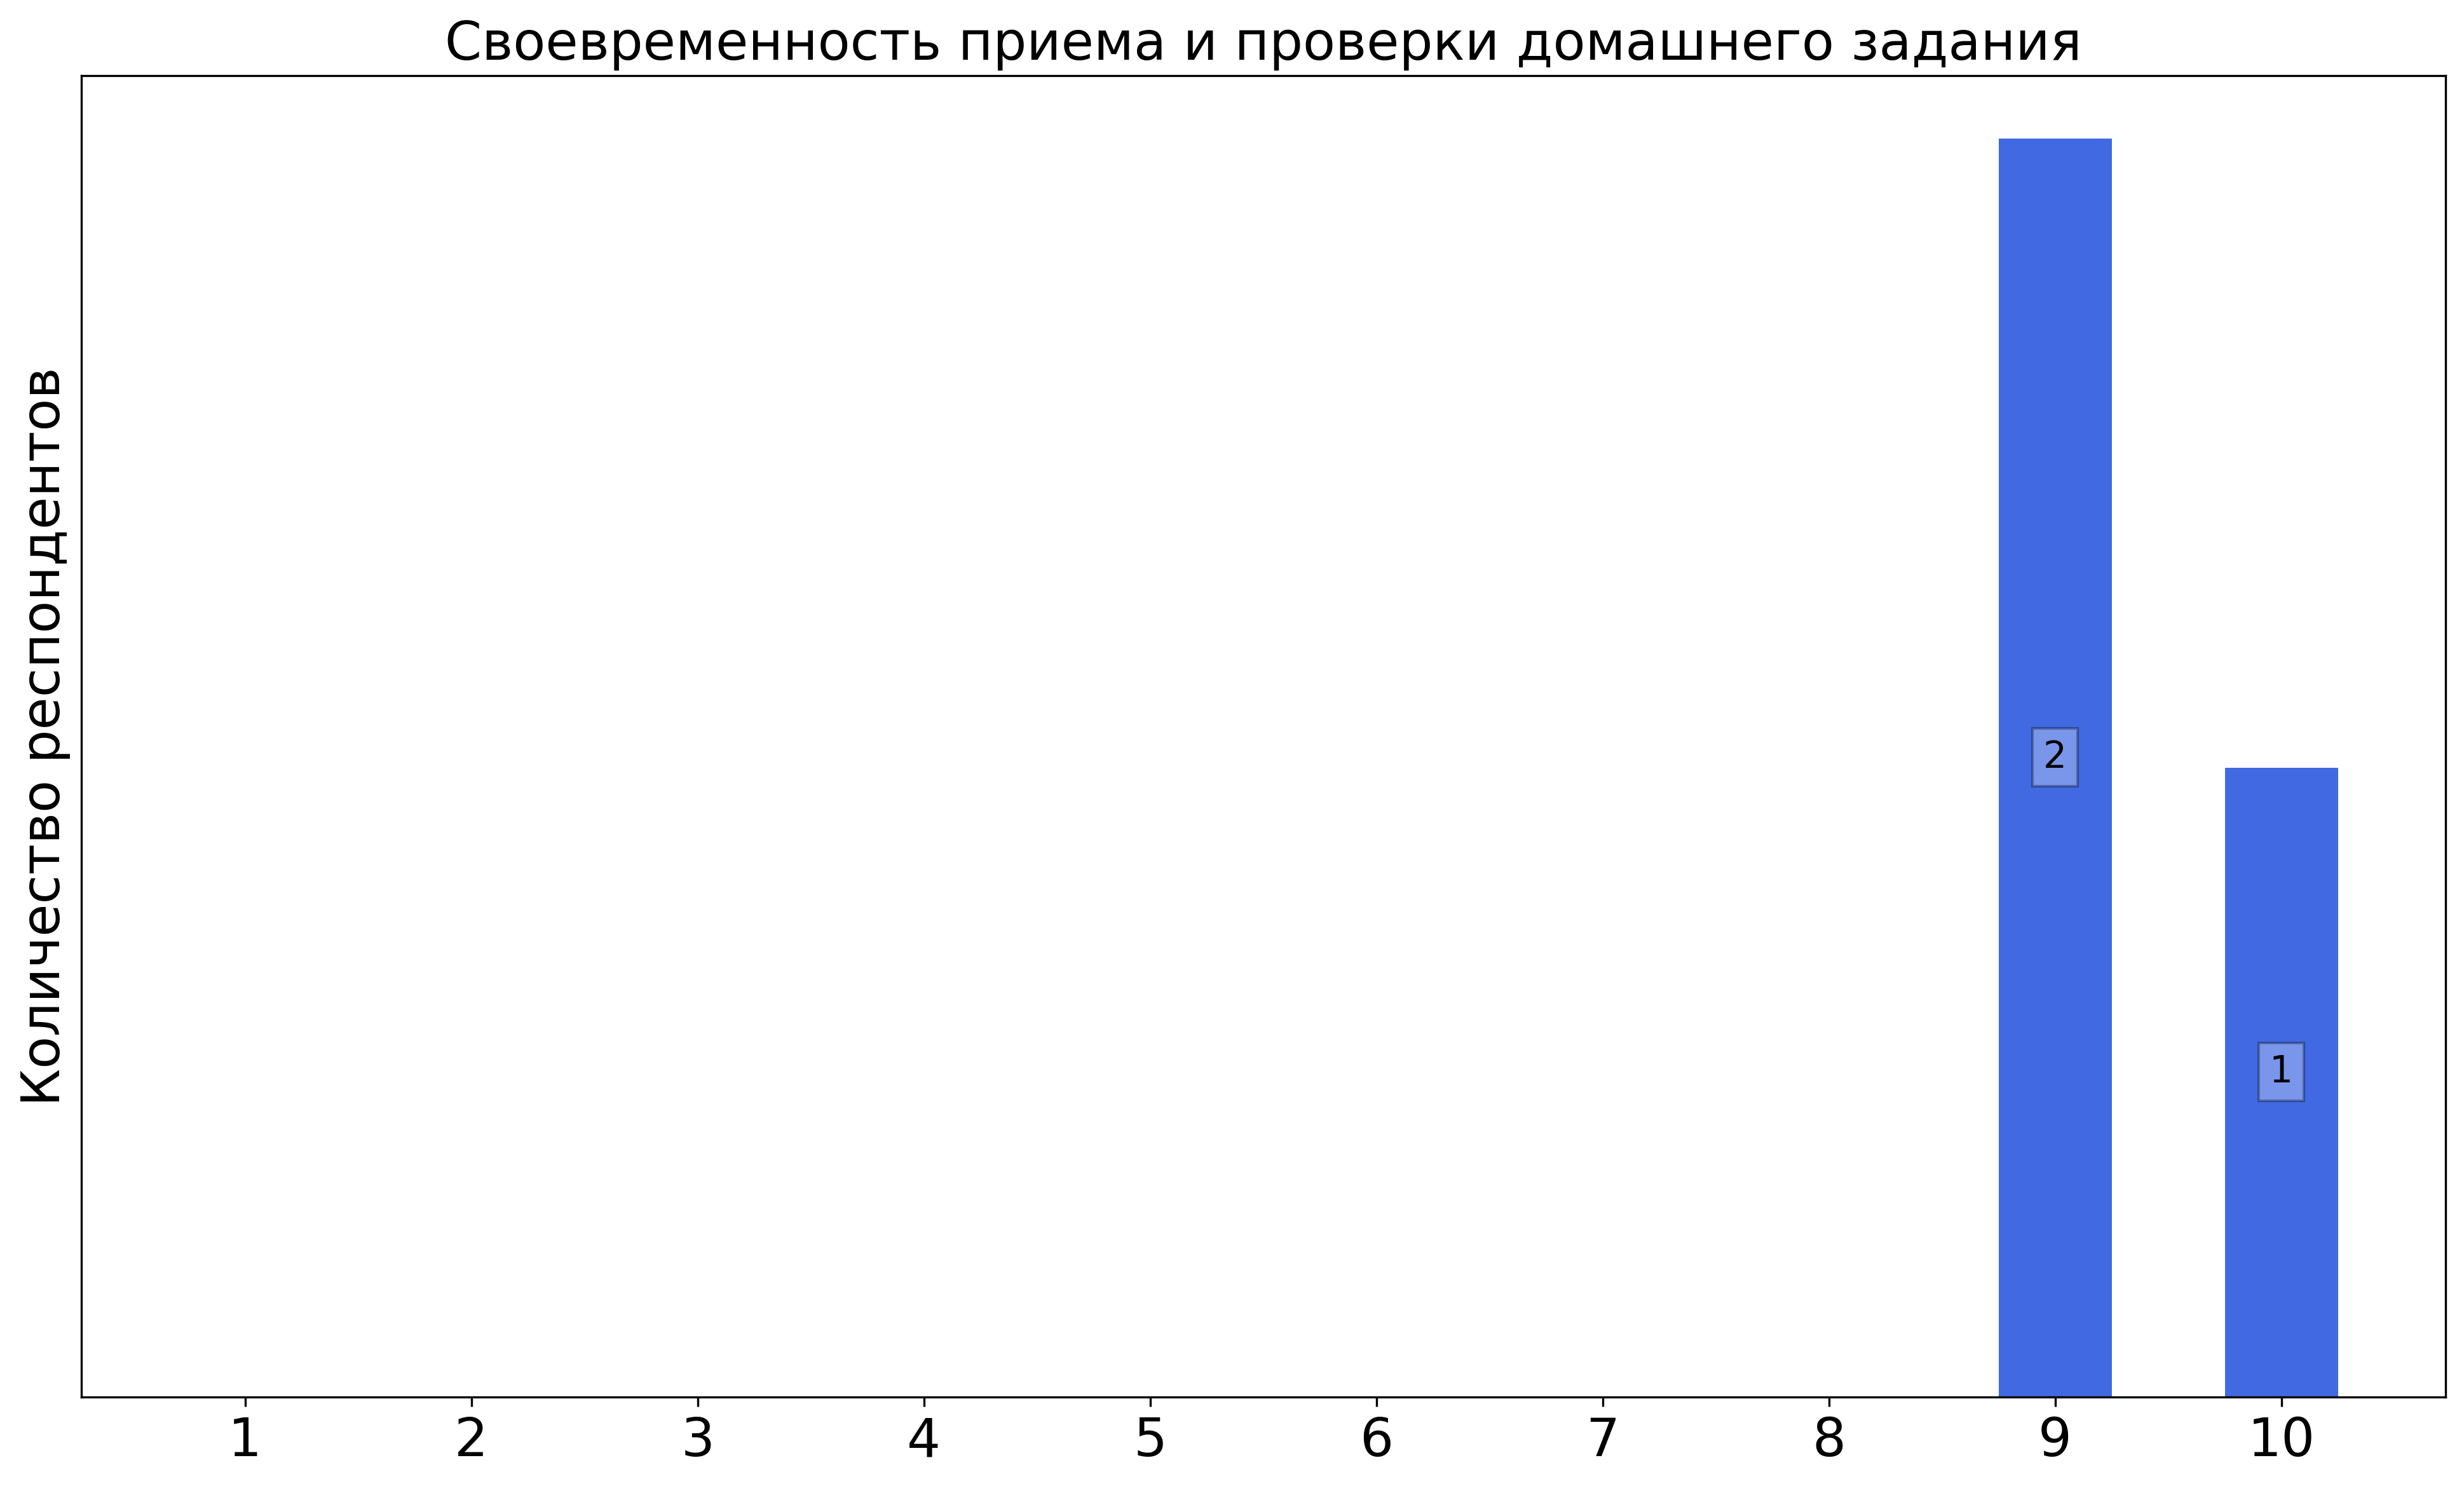
\includegraphics[width=\textwidth]{images/3 course/Общая физика - квантовая физика/seminarists-marks-Инжечик Л.В.-2.png}
                \end{subfigure}
                \begin{subfigure}[b]{0.45\textwidth}
                    \centering
                    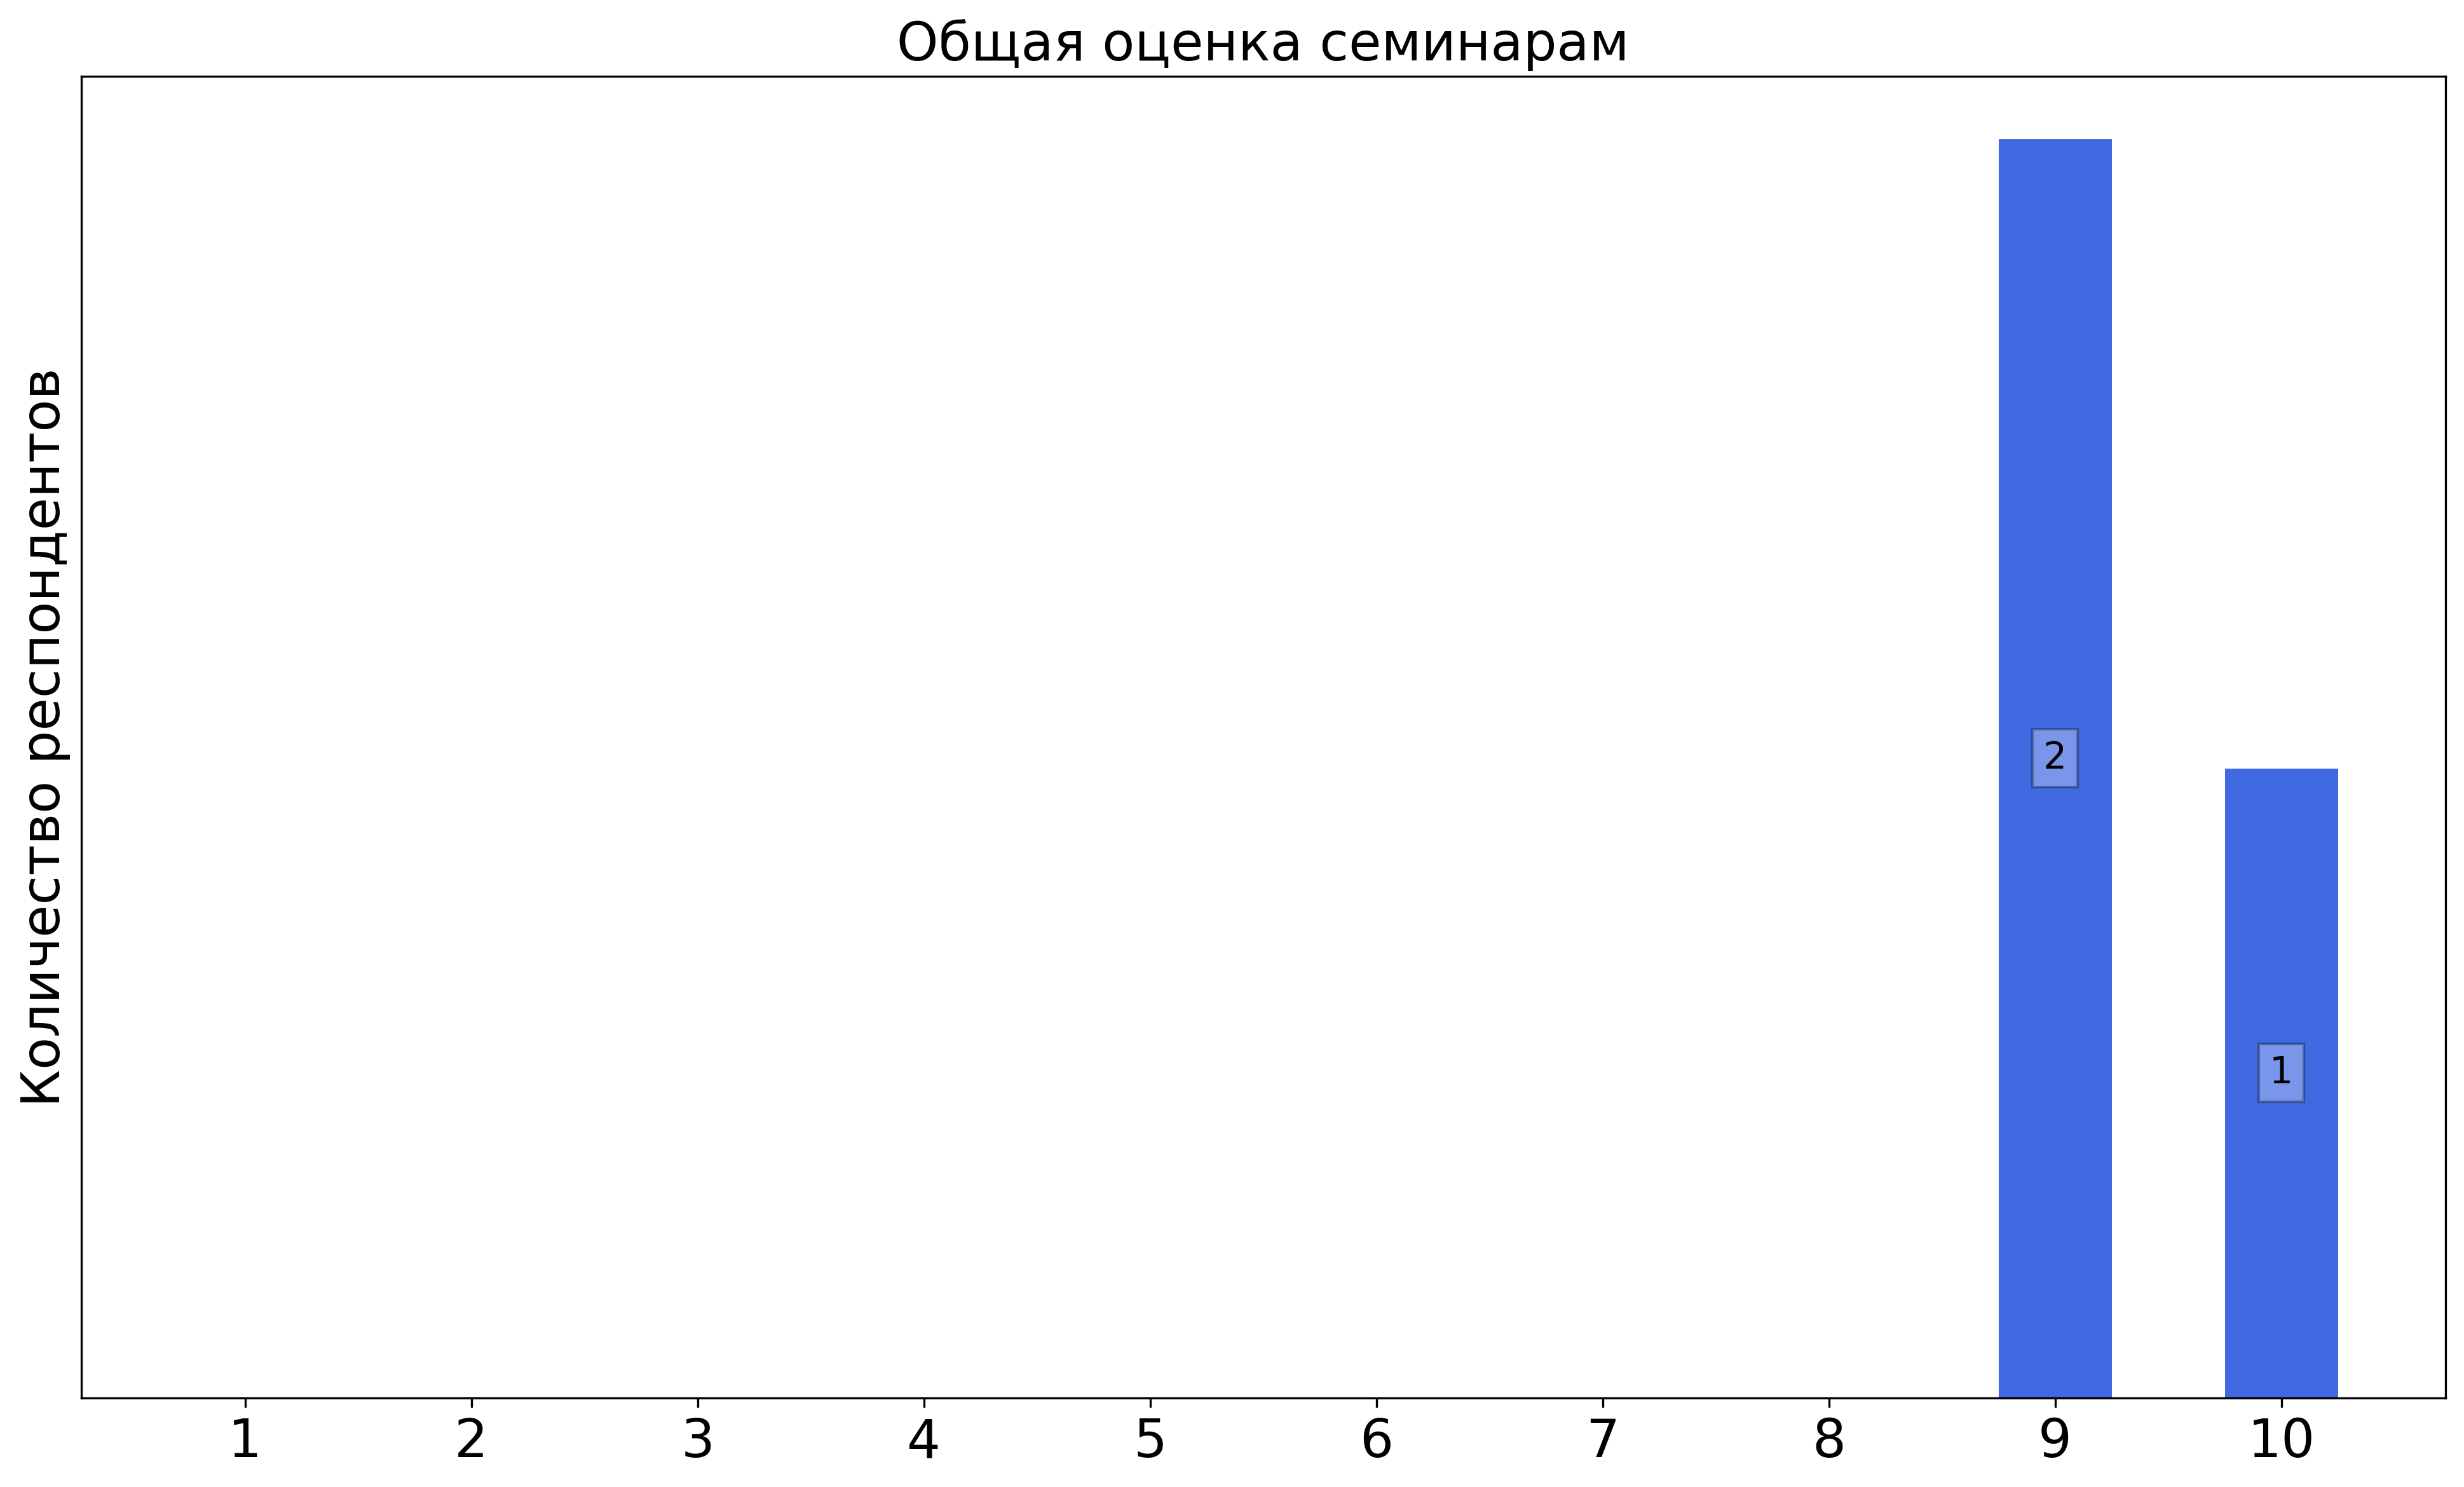
\includegraphics[width=\textwidth]{images/3 course/Общая физика - квантовая физика/seminarists-marks-Инжечик Л.В.-3.png}
                \end{subfigure}	
                \caption{Оценки респондентов о качестве преподавания семинаров}
            \end{figure}

            \textbf{Комментарии студентов о семинаристе\protect\footnote{сохранены оригинальные орфография и пунктуация}}
                \begin{commentbox} 
                    Система семинаров плоха, с точки зрения получения знаний: задачи мы по очереди решали группой. Но зато зачёт был получен холявно 
                \end{commentbox}

            
        \subsubsection{Отзыв студентов о семинарах. Семинарист: Колдунов М.Ф.}
            \begin{figure}[H]
                \centering
                \begin{subfigure}[b]{0.45\textwidth}
                    \centering
                    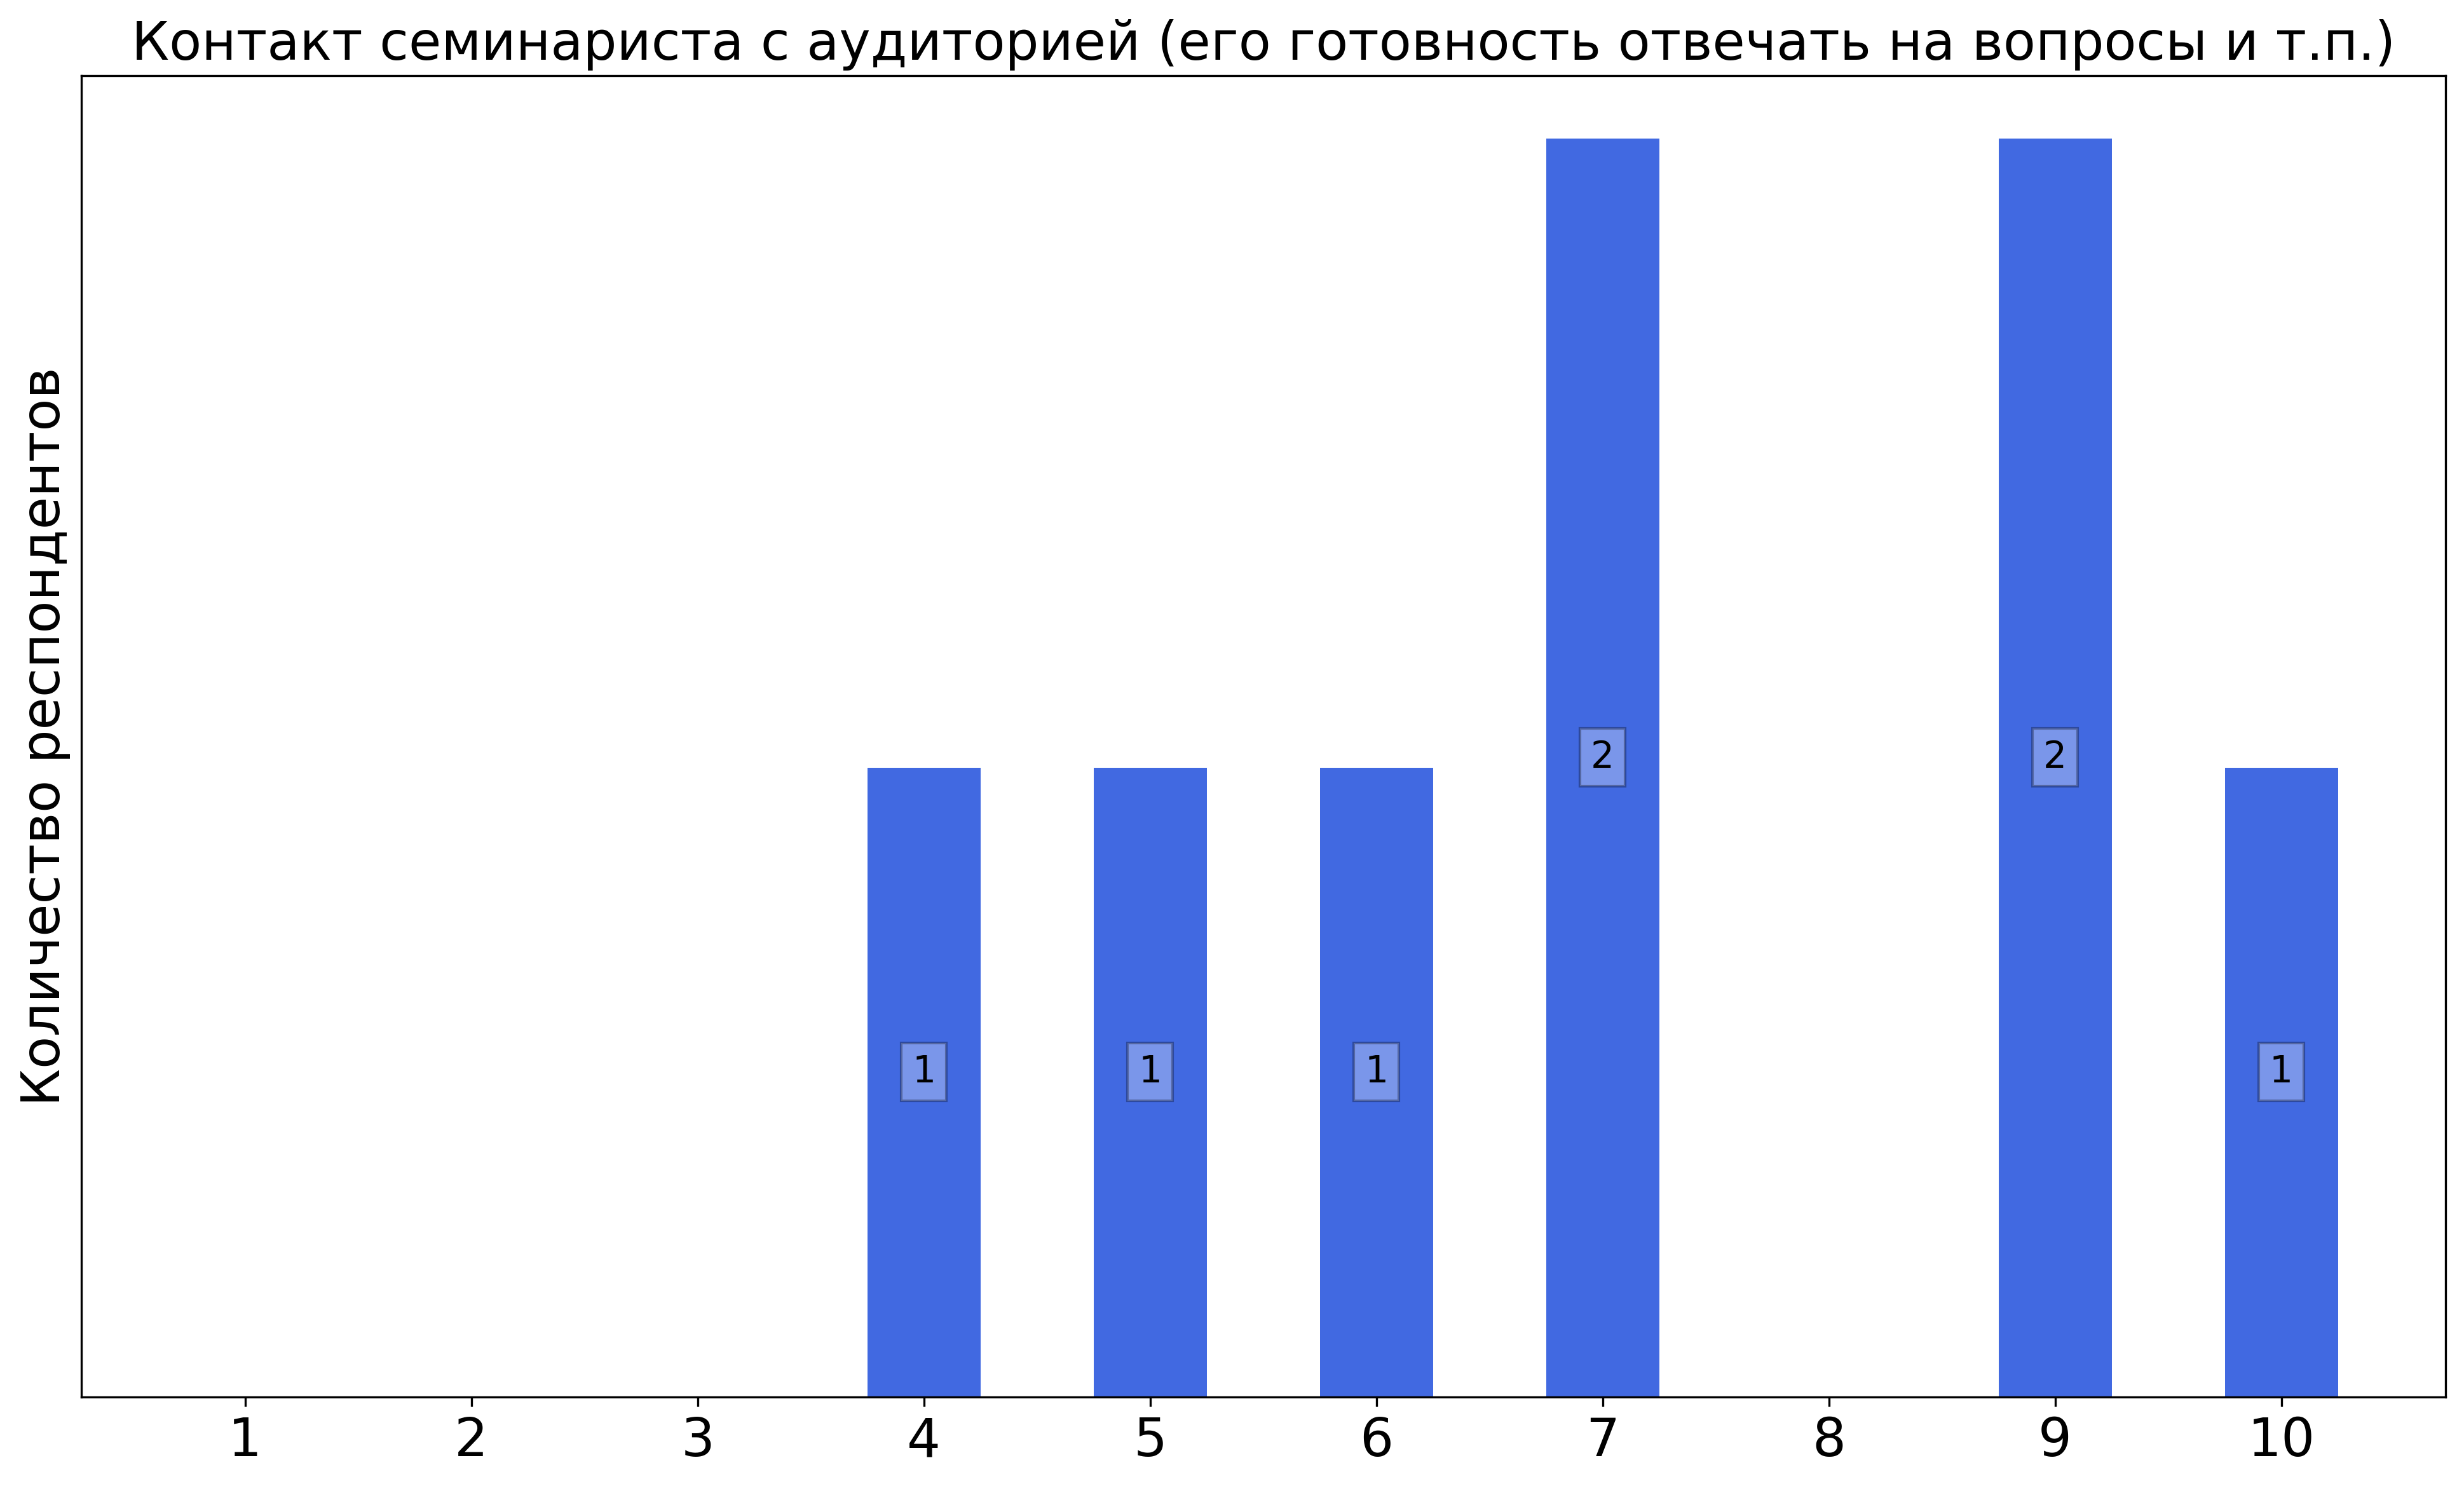
\includegraphics[width=\textwidth]{images/3 course/Общая физика - квантовая физика/seminarists-marks-Колдунов М.Ф.-0.png}
                \end{subfigure}
                \begin{subfigure}[b]{0.45\textwidth}
                    \centering
                    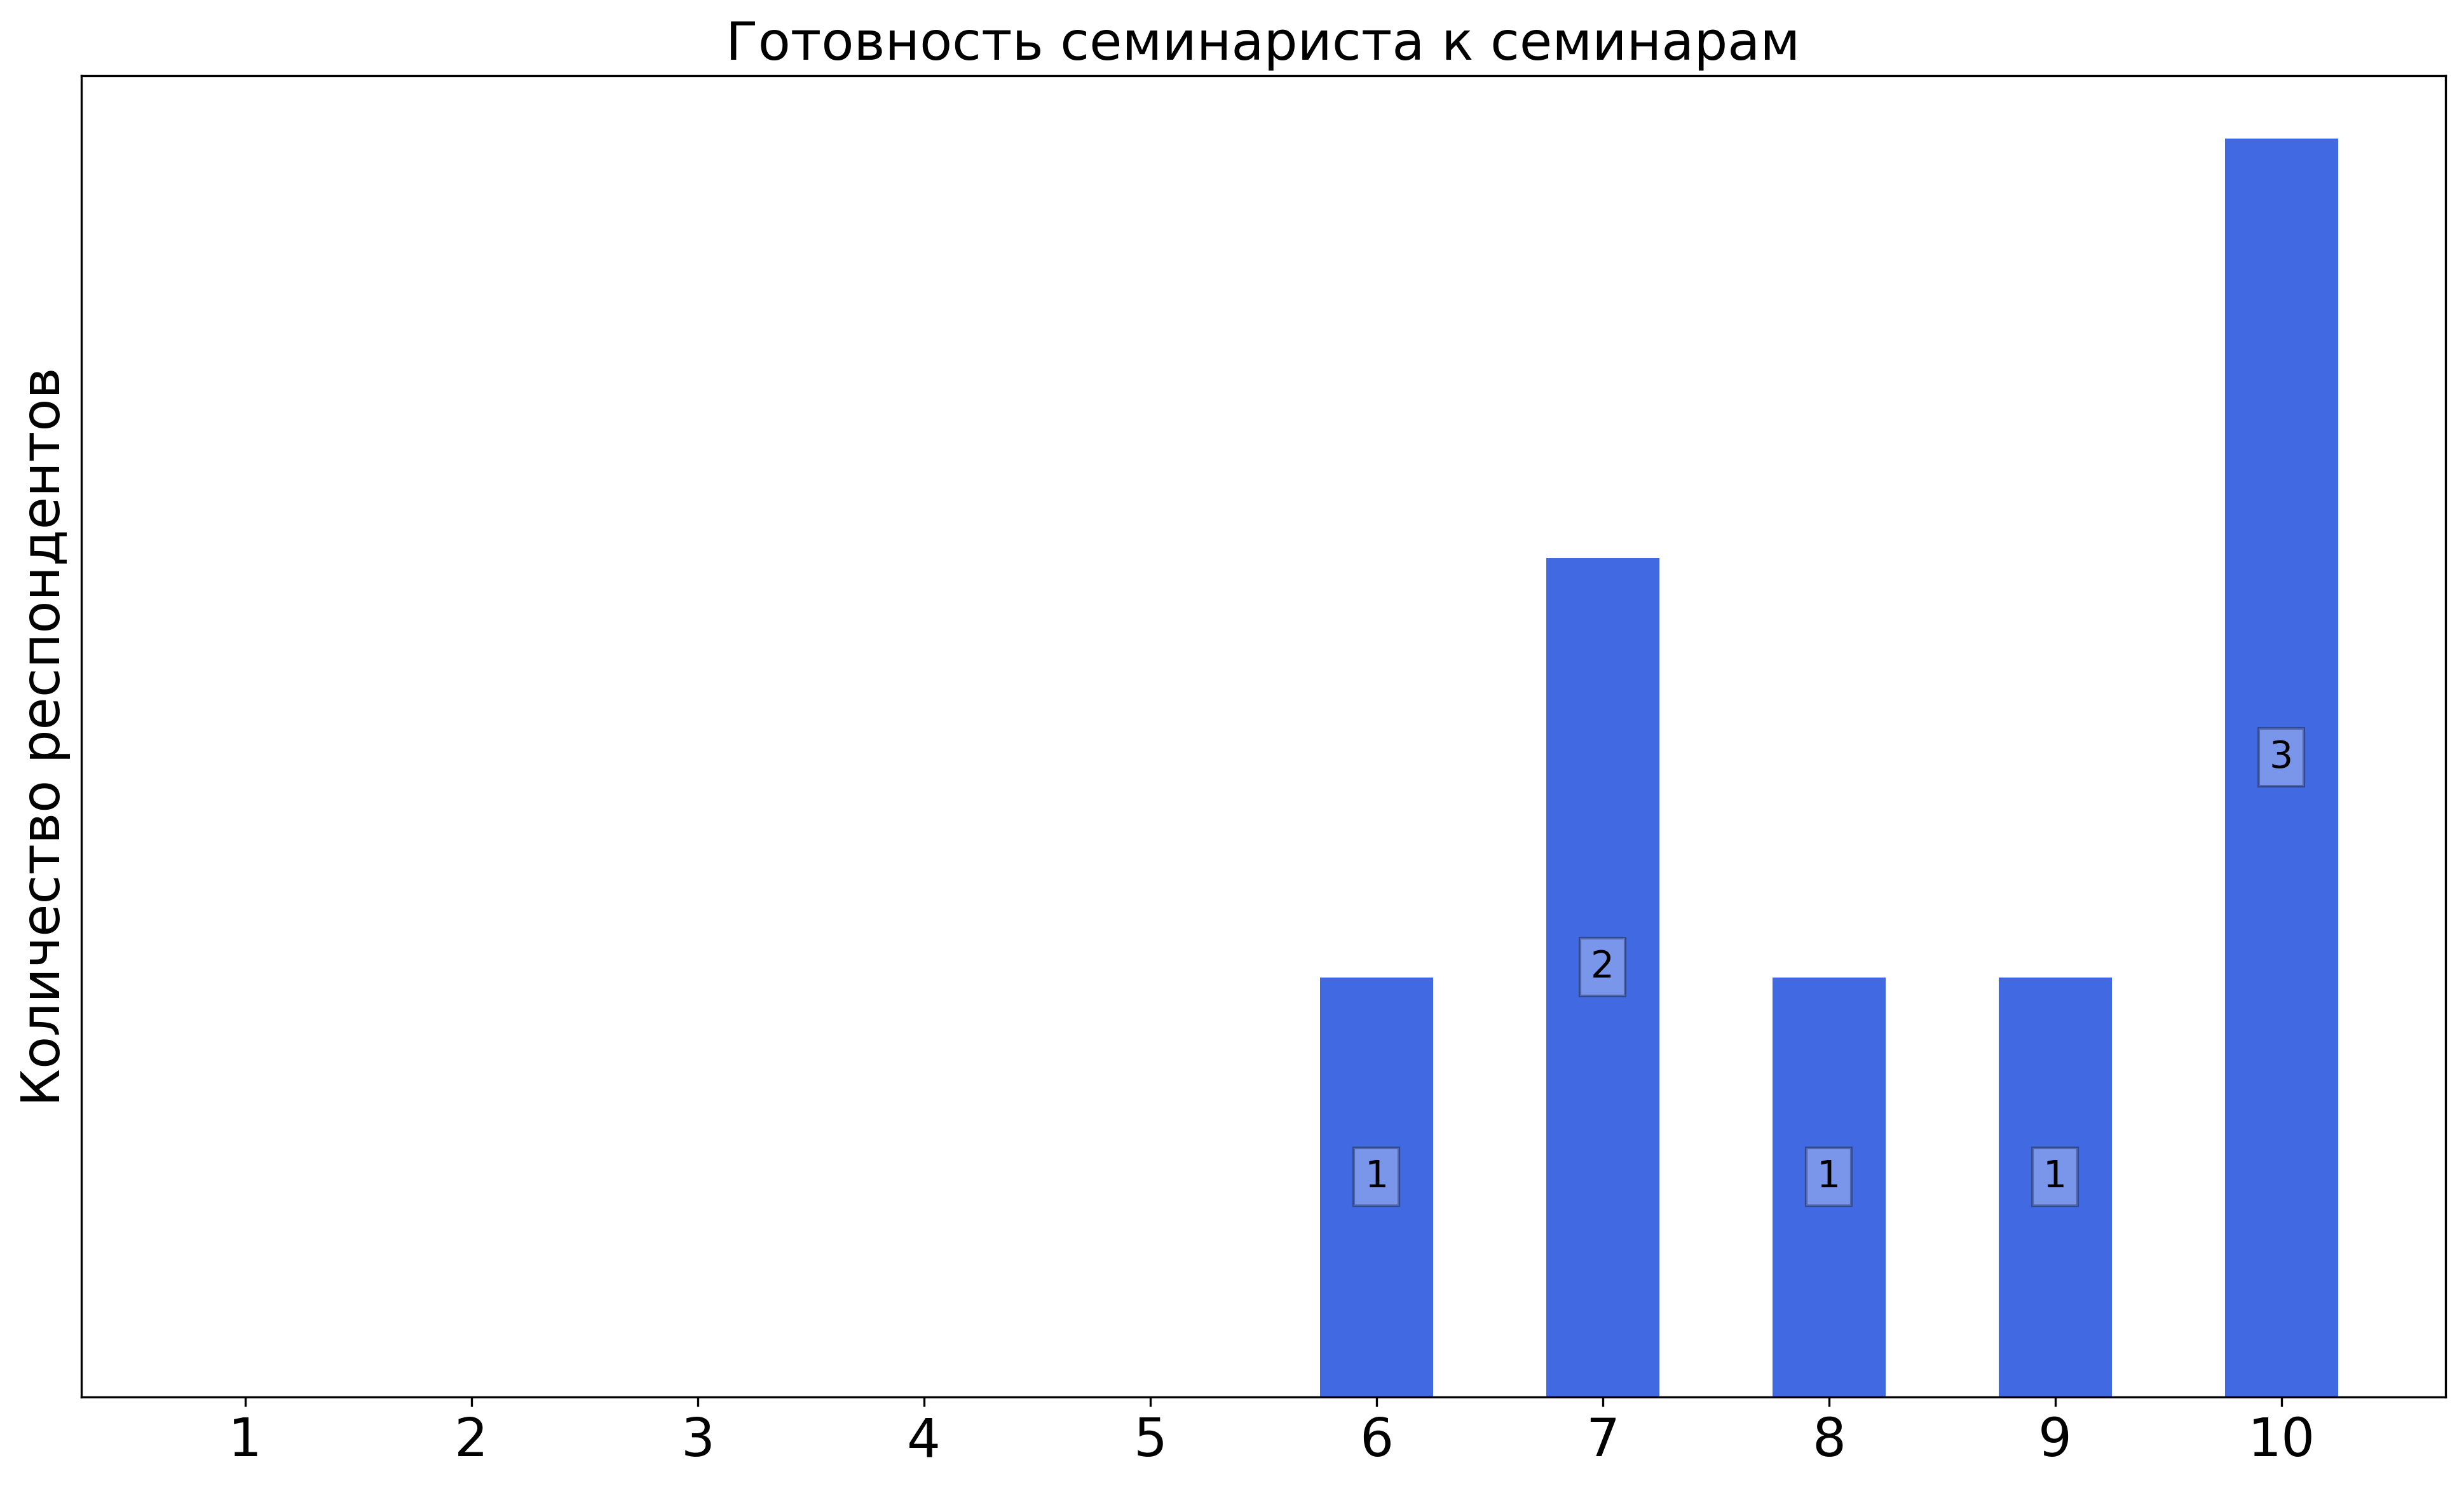
\includegraphics[width=\textwidth]{images/3 course/Общая физика - квантовая физика/seminarists-marks-Колдунов М.Ф.-1.png}
                \end{subfigure}
                \begin{subfigure}[b]{0.45\textwidth}
                    \centering
                    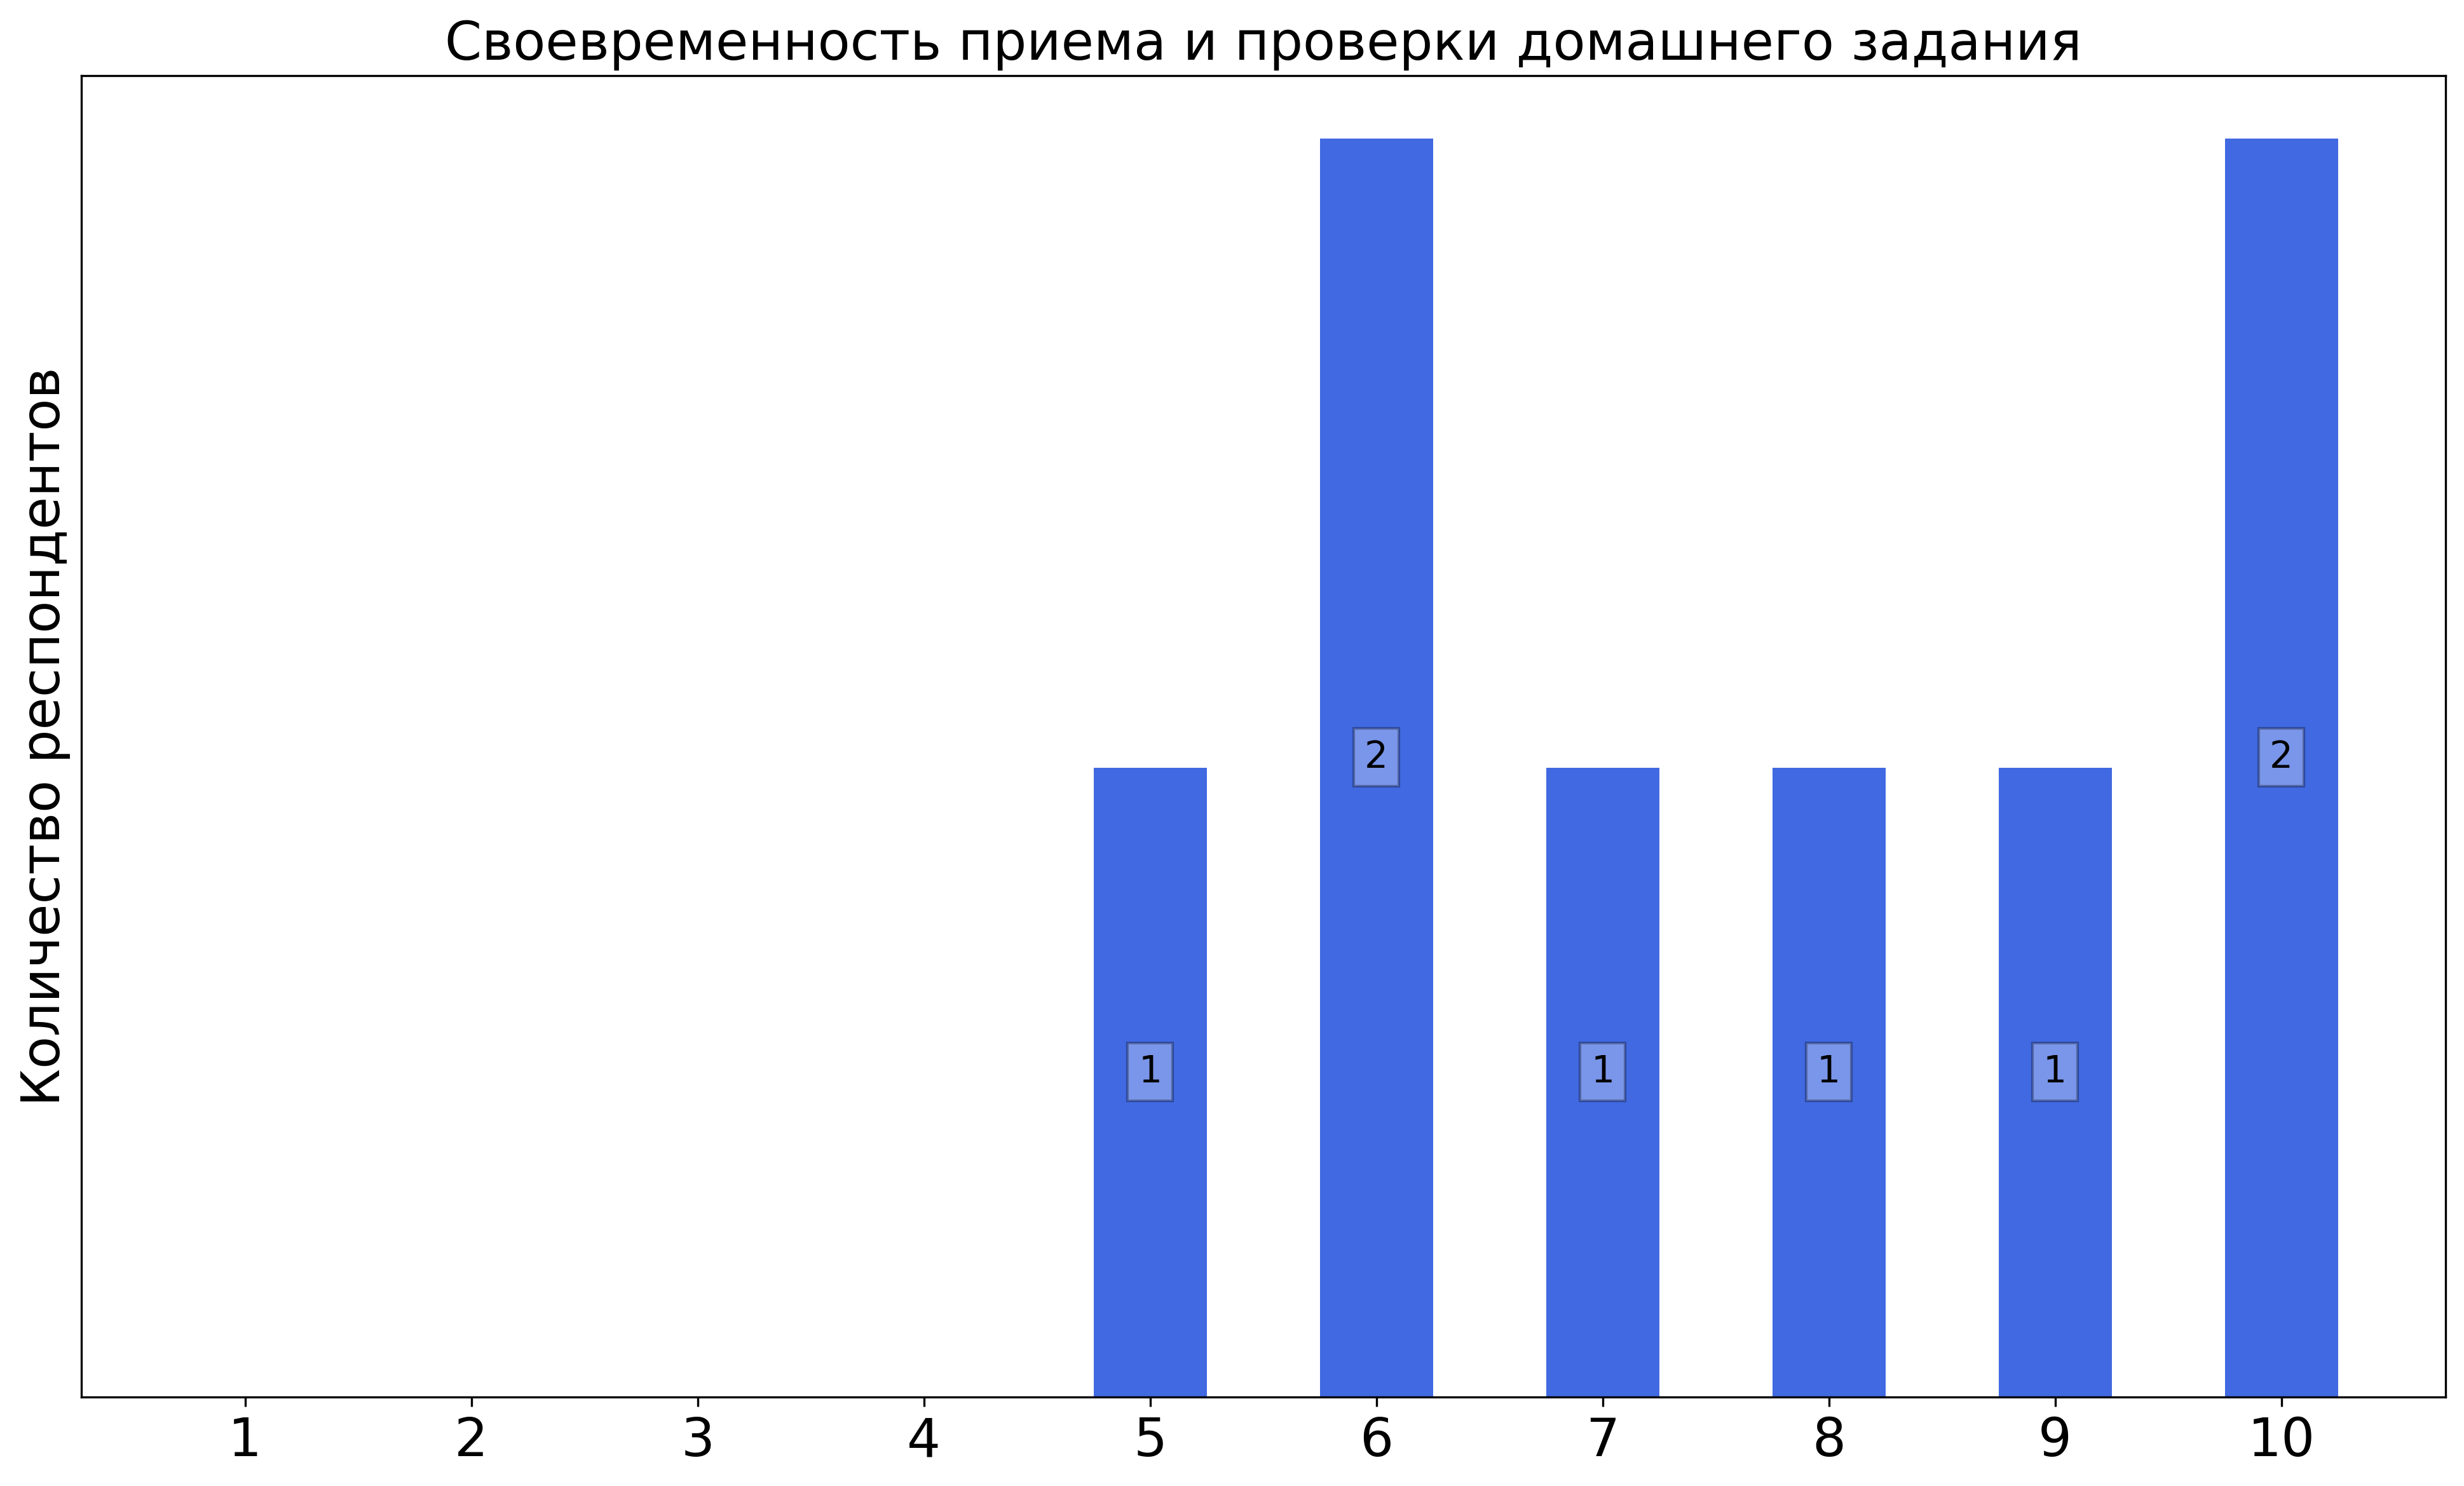
\includegraphics[width=\textwidth]{images/3 course/Общая физика - квантовая физика/seminarists-marks-Колдунов М.Ф.-2.png}
                \end{subfigure}
                \begin{subfigure}[b]{0.45\textwidth}
                    \centering
                    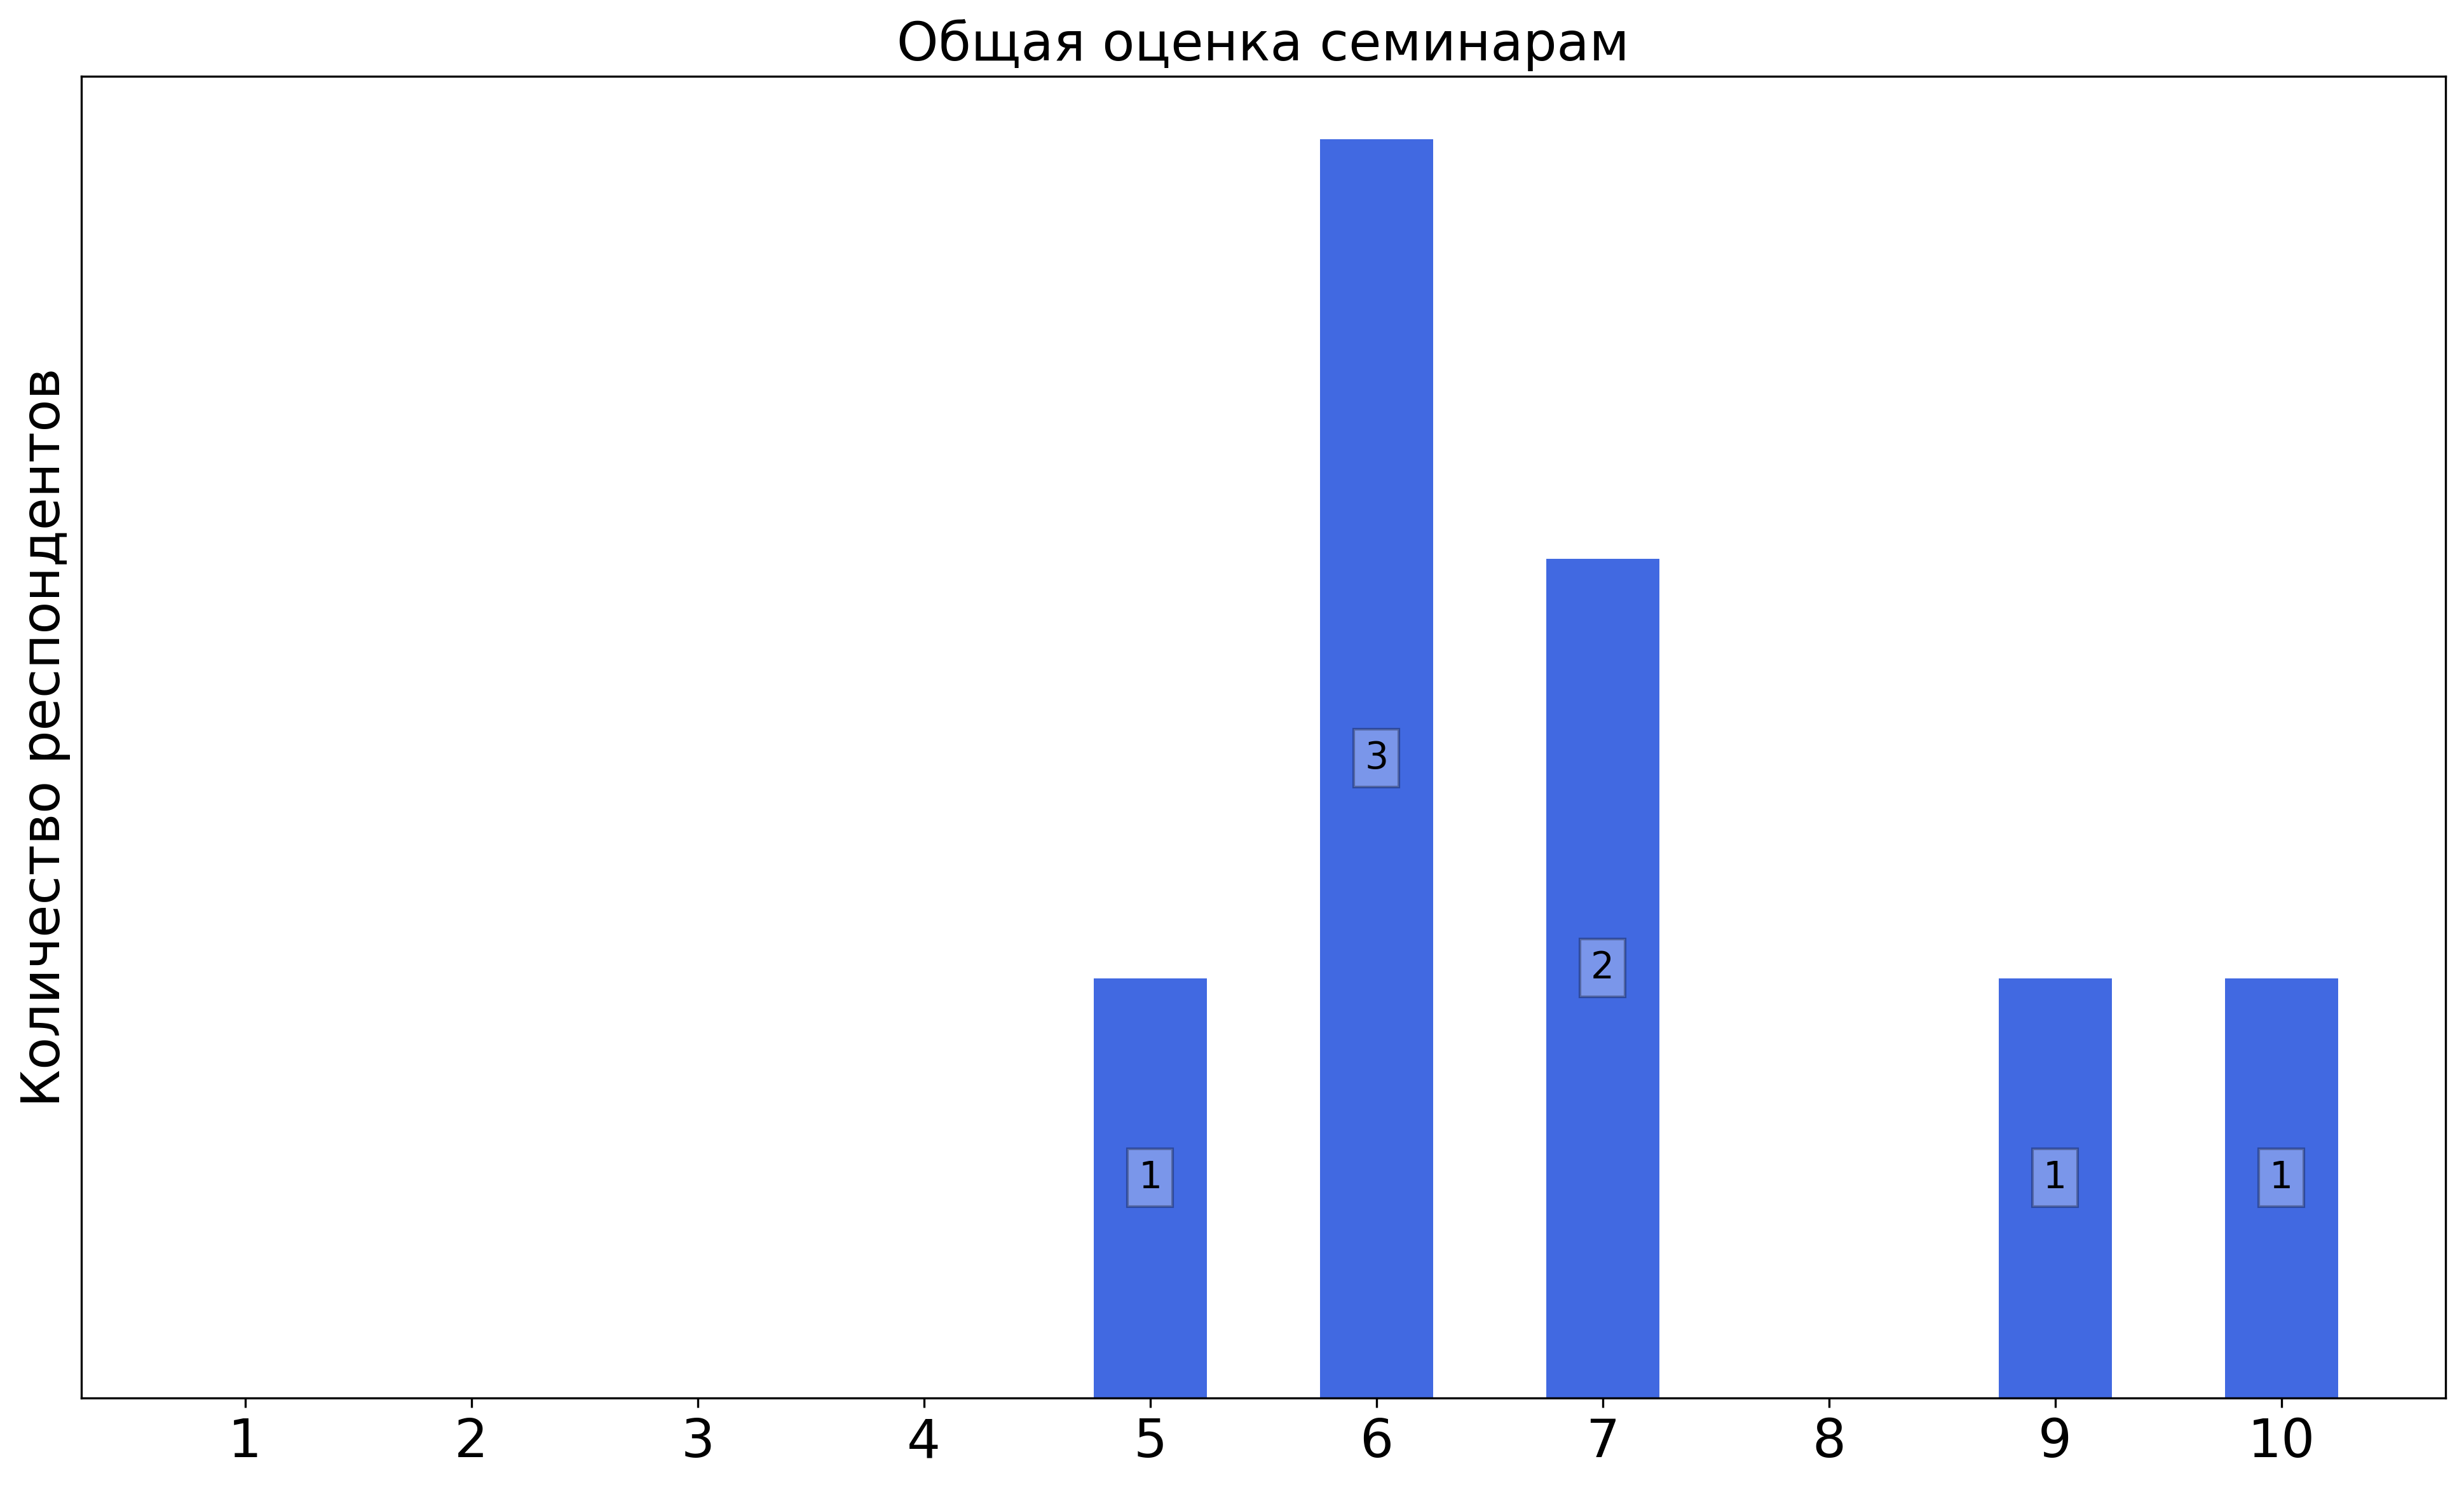
\includegraphics[width=\textwidth]{images/3 course/Общая физика - квантовая физика/seminarists-marks-Колдунов М.Ф.-3.png}
                \end{subfigure}	
                \caption{Оценки респондентов о качестве преподавания семинаров}
            \end{figure}

            \textbf{Комментарии студентов о семинаристе\protect\footnote{сохранены оригинальные орфография и пунктуация}}
                \begin{commentbox} 
                    Очень разбирающийся преподаватель. Но темп, который он задаёт, очень быстрый для студентов 
                \end{commentbox} 
            
                \begin{commentbox} 
                    К сожалению, было очень плохо понятно, что происходит. Он очень хорошо с нами взаимодействовал, иногда развлекал нас, чтобы нам было не слишком тяжко, но я едва понимал, что происходит. Впрочем тут может проблема быть и во мне 
                \end{commentbox} 
            
                \begin{commentbox} 
                    Знает по предмету очень много, правда, иногда это бывает не на пользу, поскольку Колдунов излагать строго и использовать аппарат теоретической физики (в этом случае, понятное дело, имеется в виду квантовая механика), а на ФРКТ этот предмет начинается только в 6 семестре. В общем, зачастую получается довольно мудрёно для общей физики. Контрольные работы довольно непростые, хоть и оценивается не так строго (например, как вам потенциальный барьер в виде дельта-функции?). В итоге ощущения получаются довольно смешанные. 
                \end{commentbox} 
            
                \begin{commentbox} 
                    Нормальный, не знаю как его еще описать. Во многом, как мне показалось, человек настроения. Принимал зачеты довольно лояльно, но чтобы получить отл - должно повести с настроением преподавателя.
                \end{commentbox} 


        \subsubsection{Отзыв студентов о семинарах. Семинарист: Кубышкин А.В.}
            \begin{figure}[H]
                \centering
                \begin{subfigure}[b]{0.45\textwidth}
                    \centering
                    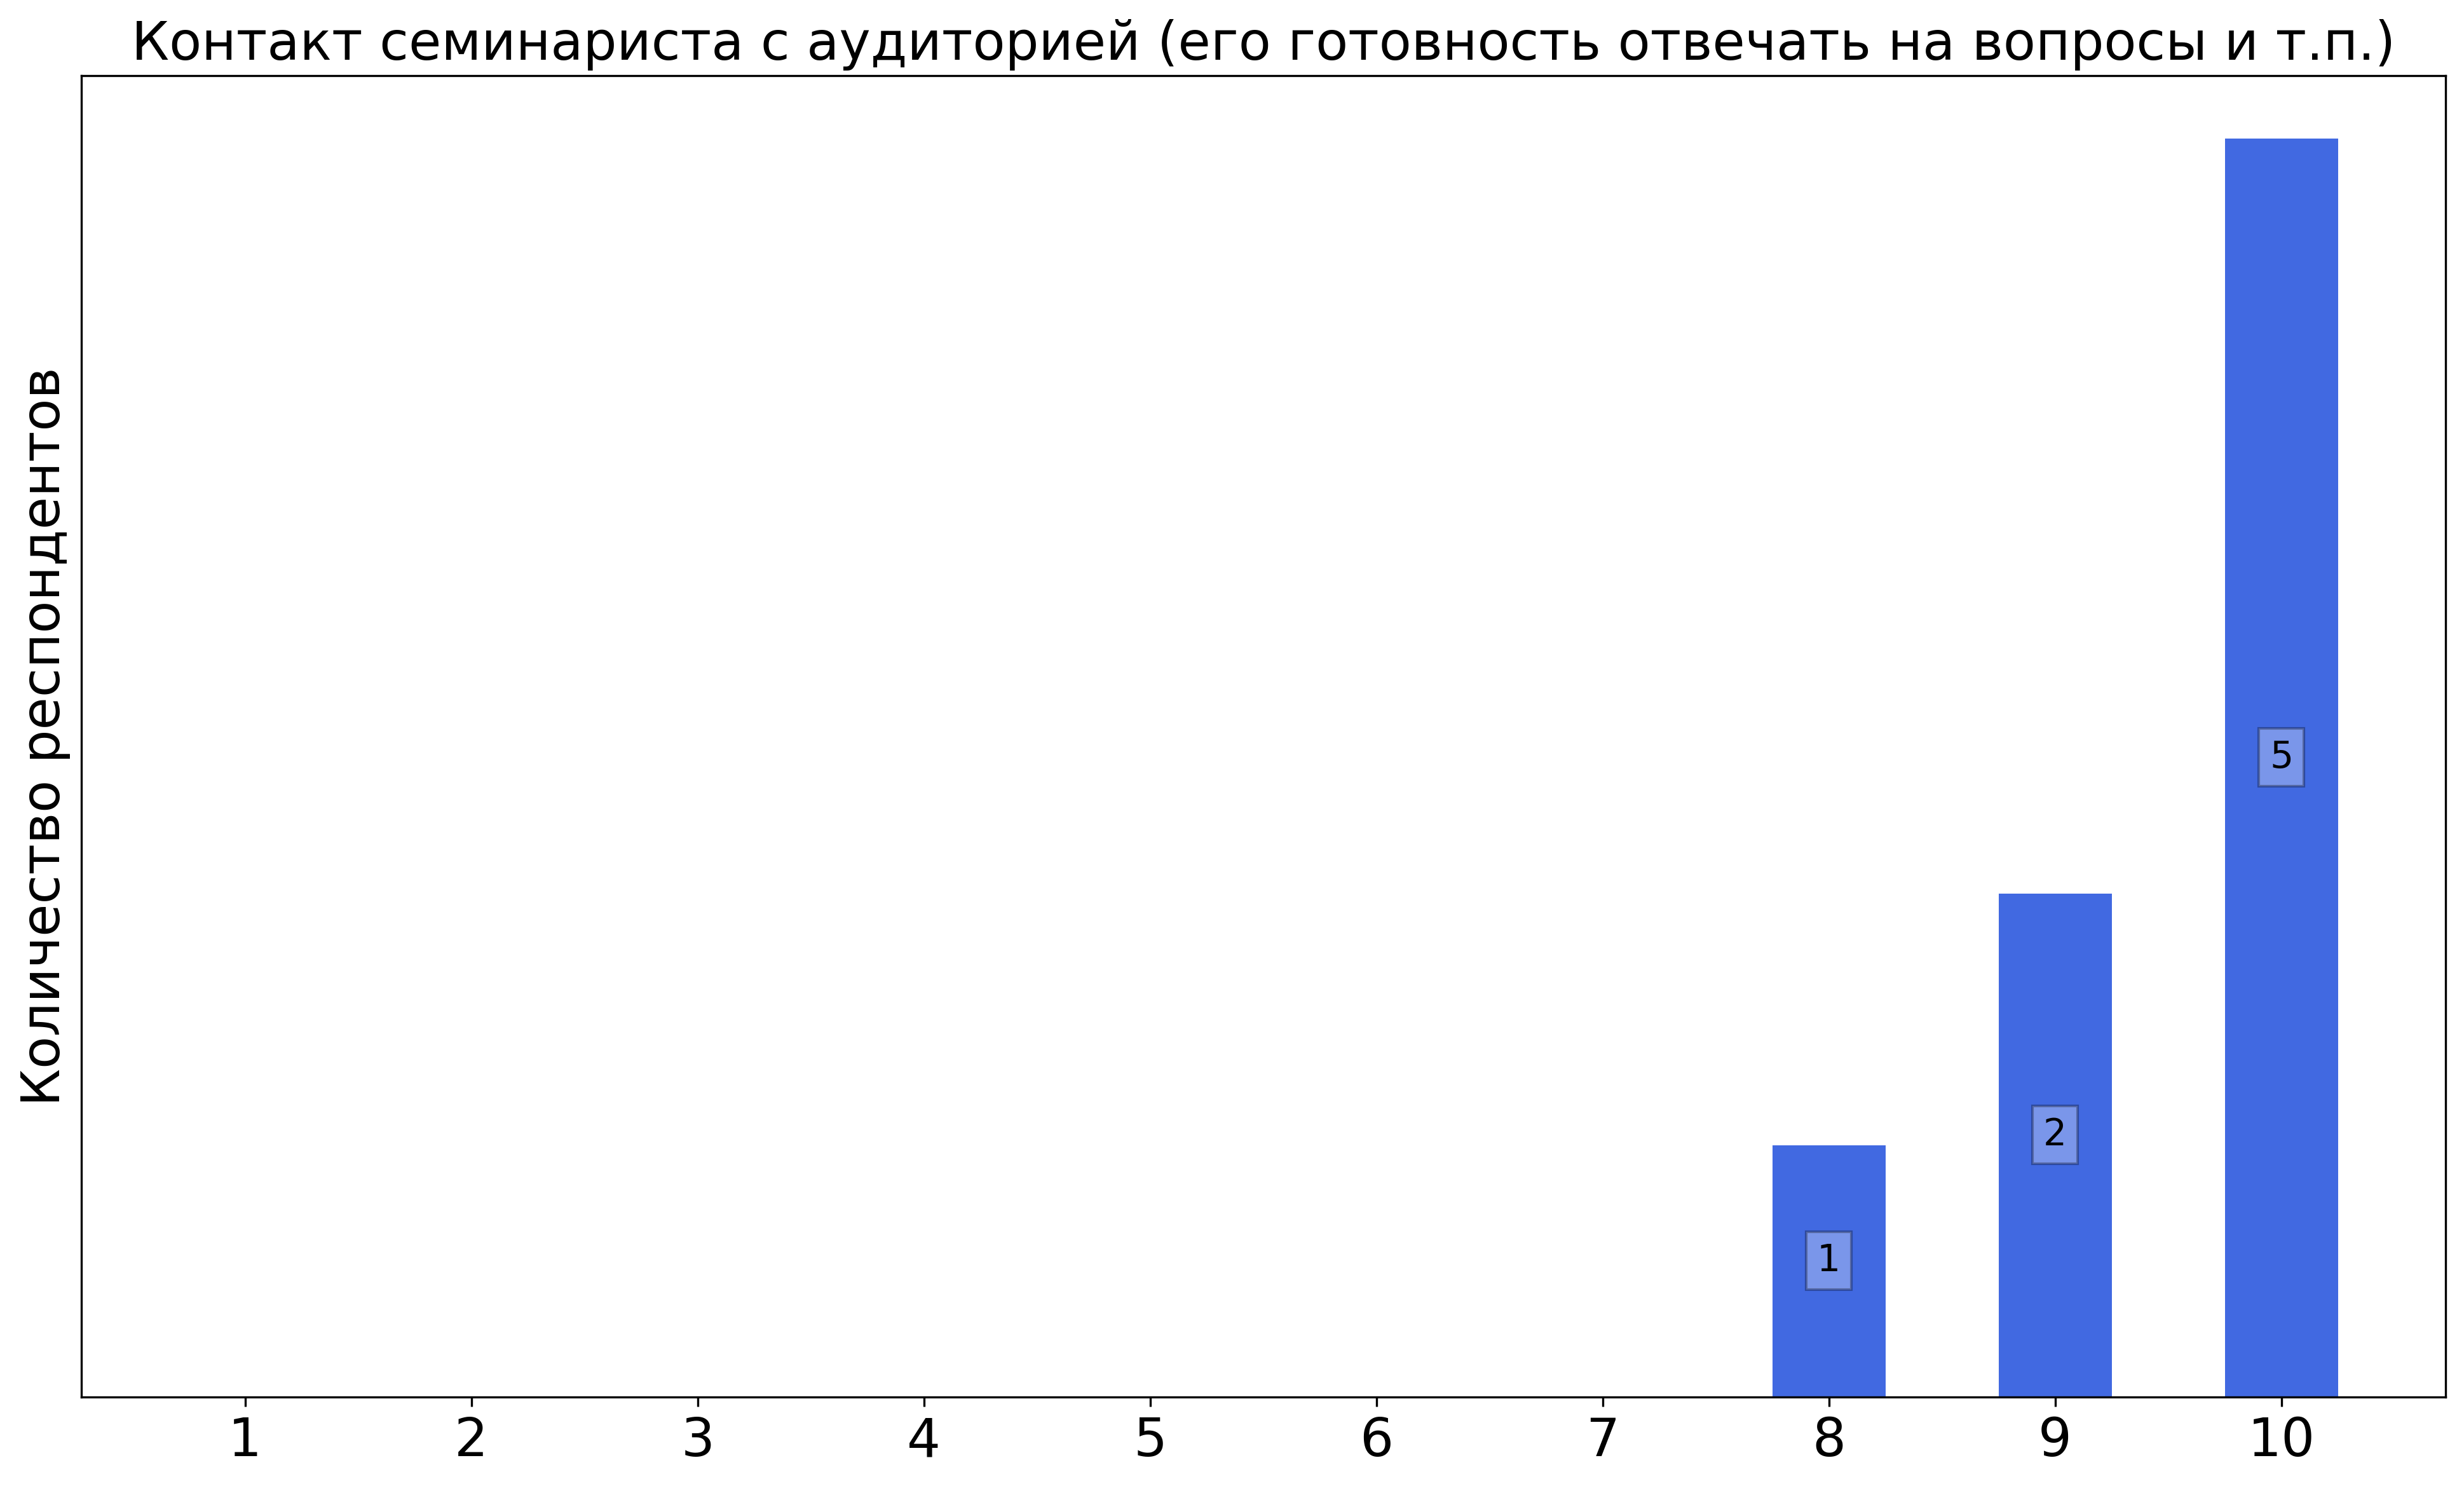
\includegraphics[width=\textwidth]{images/3 course/Общая физика - квантовая физика/seminarists-marks-Кубышкин А.В.-0.png}
                \end{subfigure}
                \begin{subfigure}[b]{0.45\textwidth}
                    \centering
                    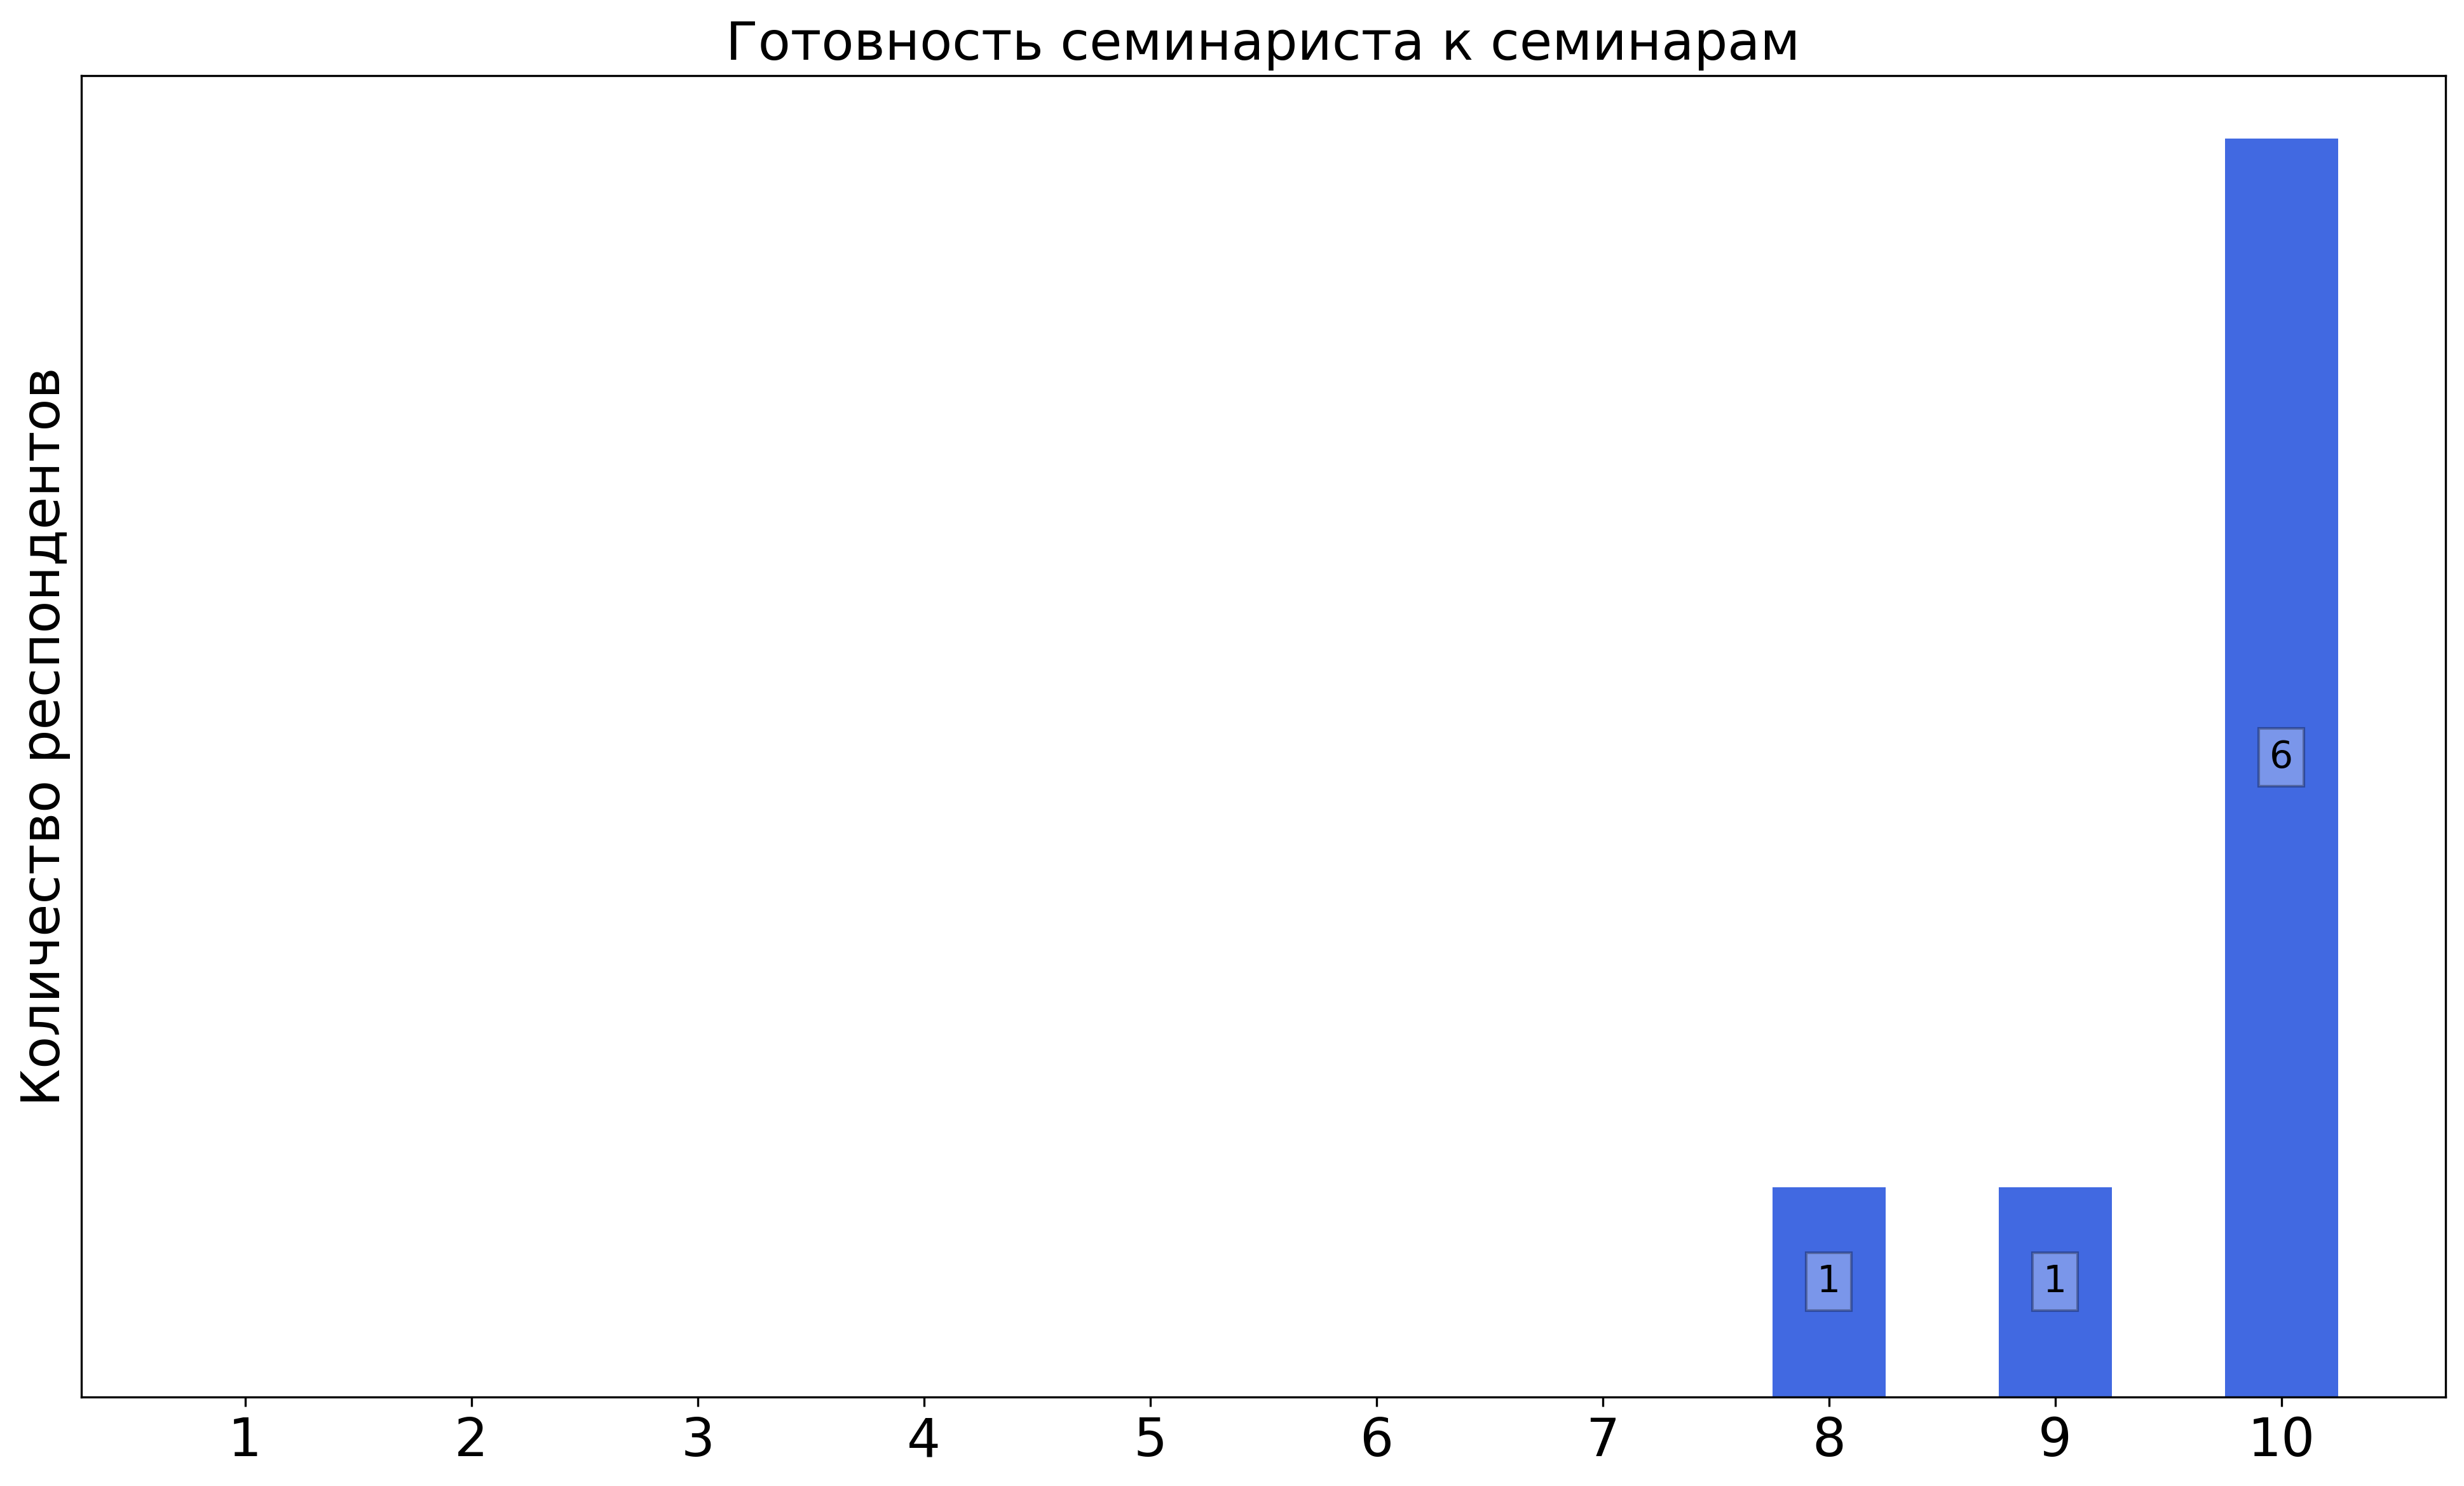
\includegraphics[width=\textwidth]{images/3 course/Общая физика - квантовая физика/seminarists-marks-Кубышкин А.В.-1.png}
                \end{subfigure}
                \begin{subfigure}[b]{0.45\textwidth}
                    \centering
                    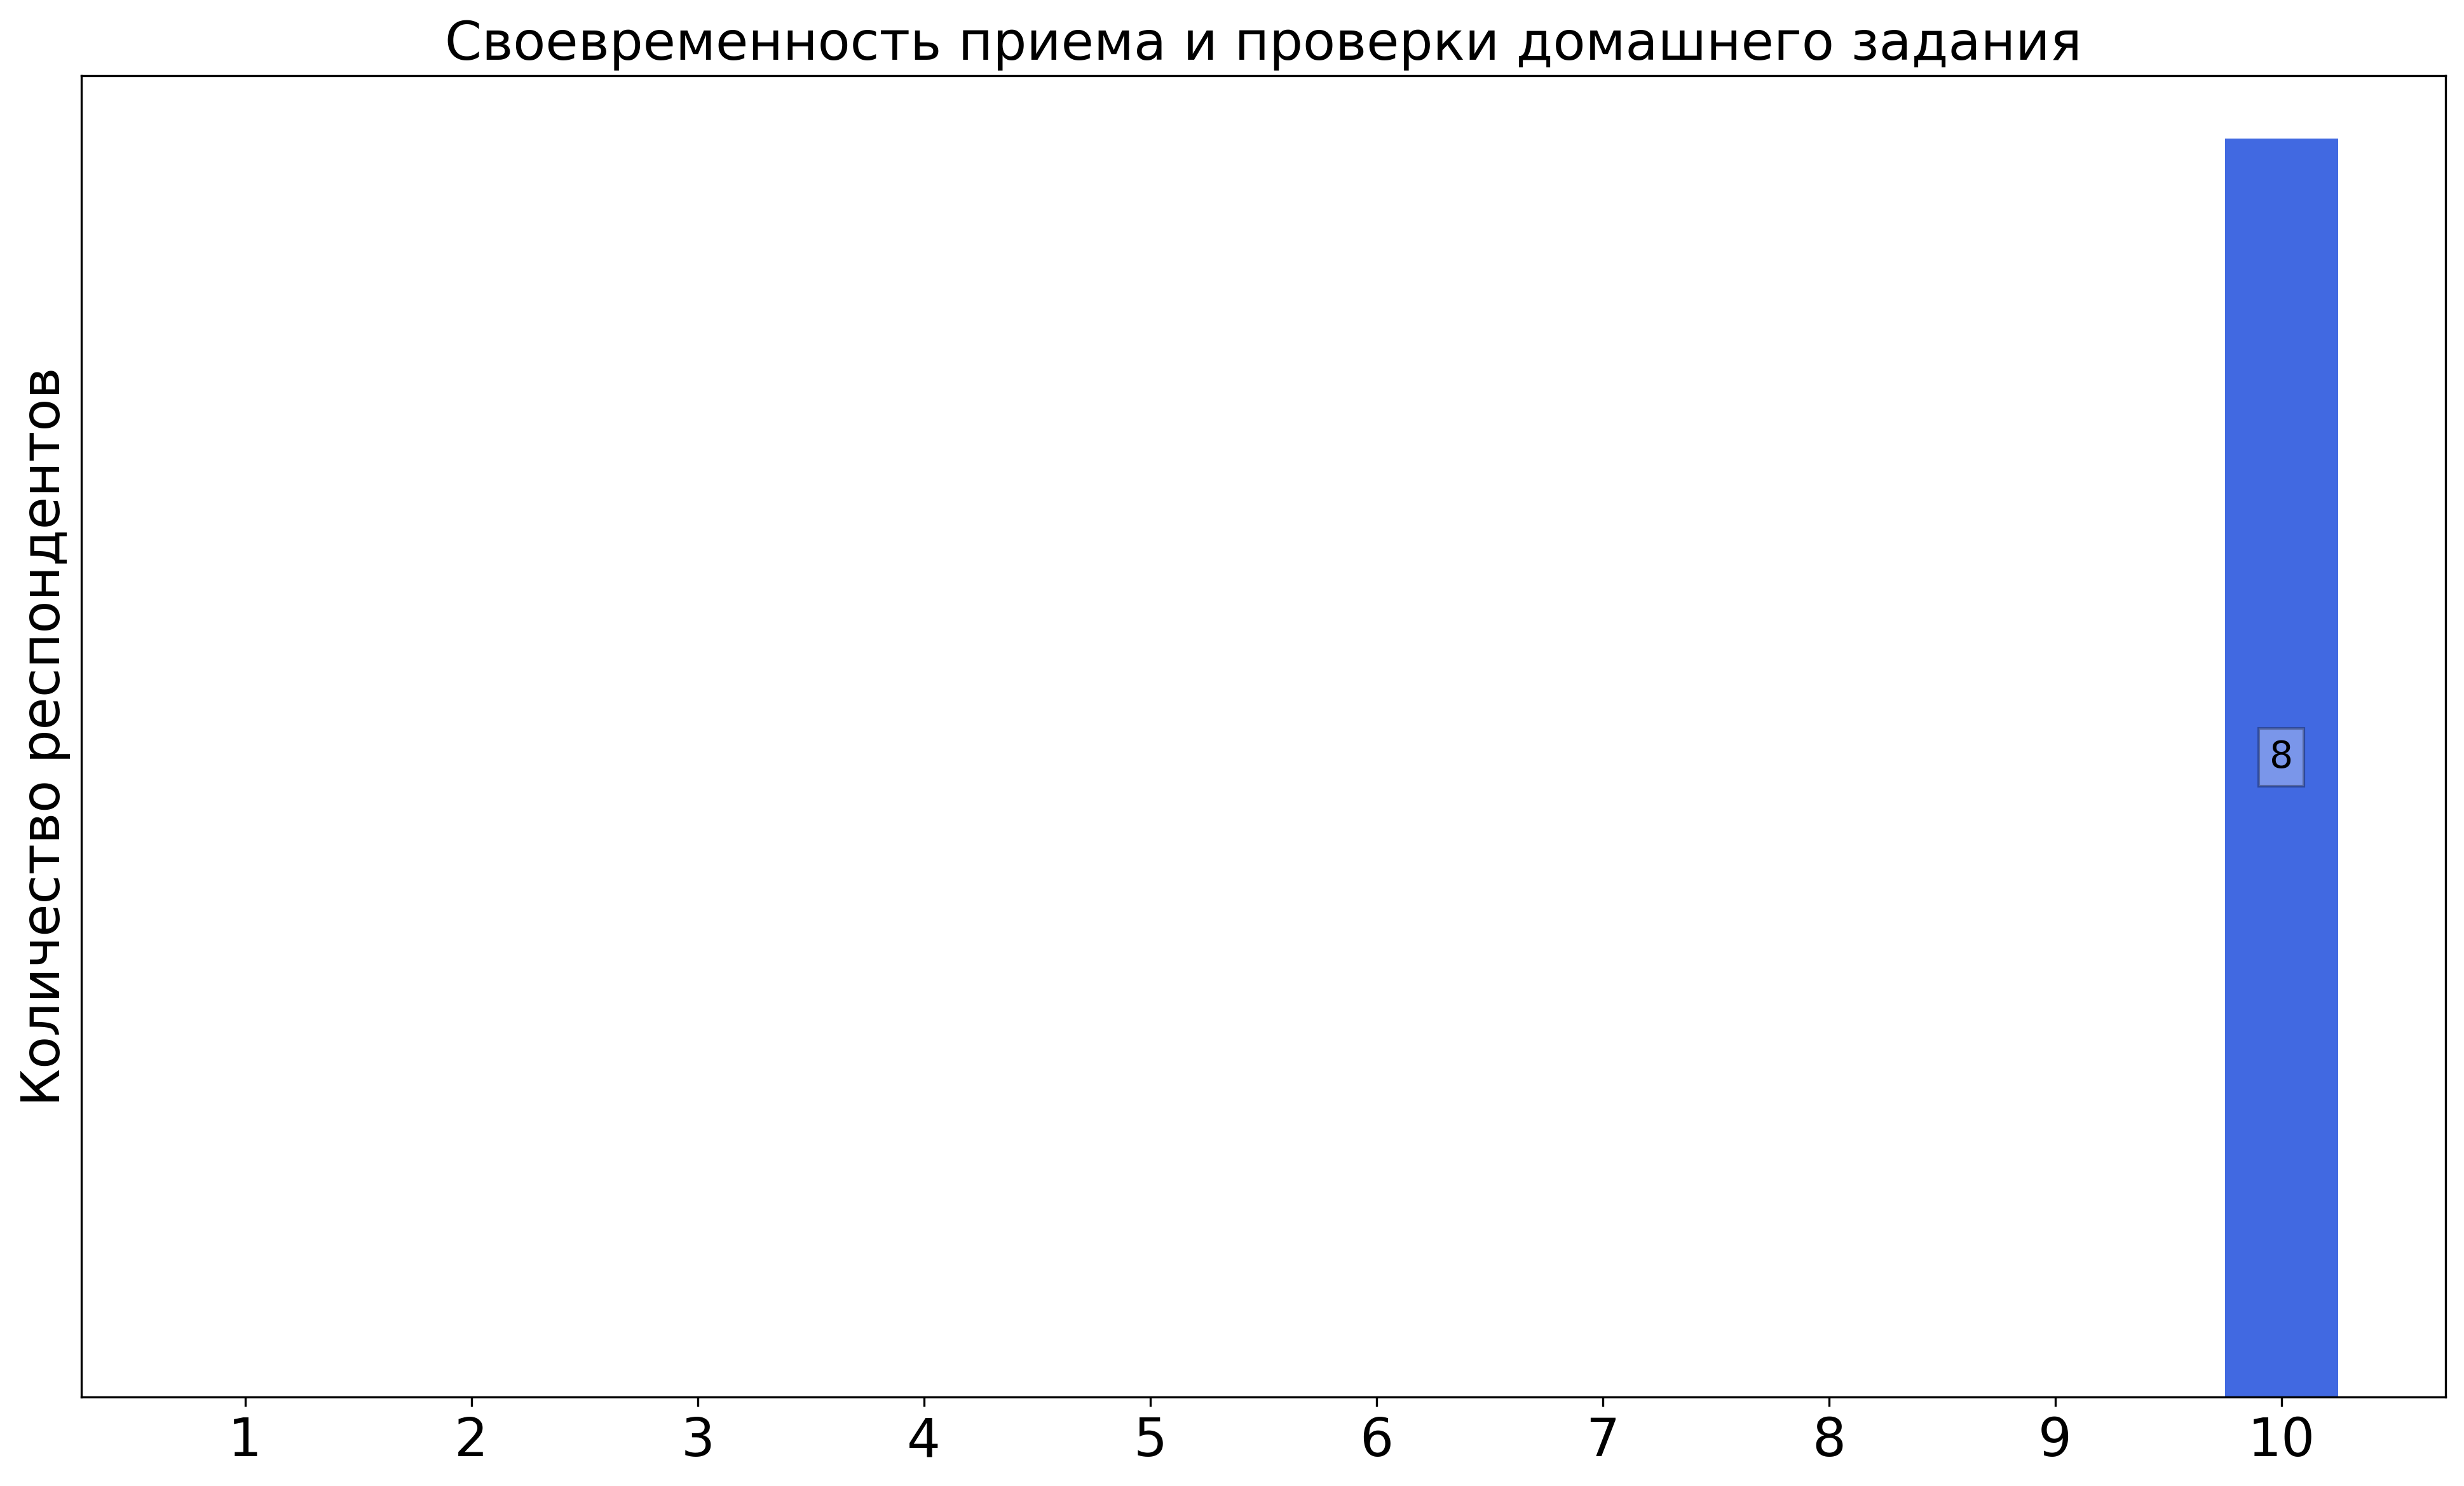
\includegraphics[width=\textwidth]{images/3 course/Общая физика - квантовая физика/seminarists-marks-Кубышкин А.В.-2.png}
                \end{subfigure}
                \begin{subfigure}[b]{0.45\textwidth}
                    \centering
                    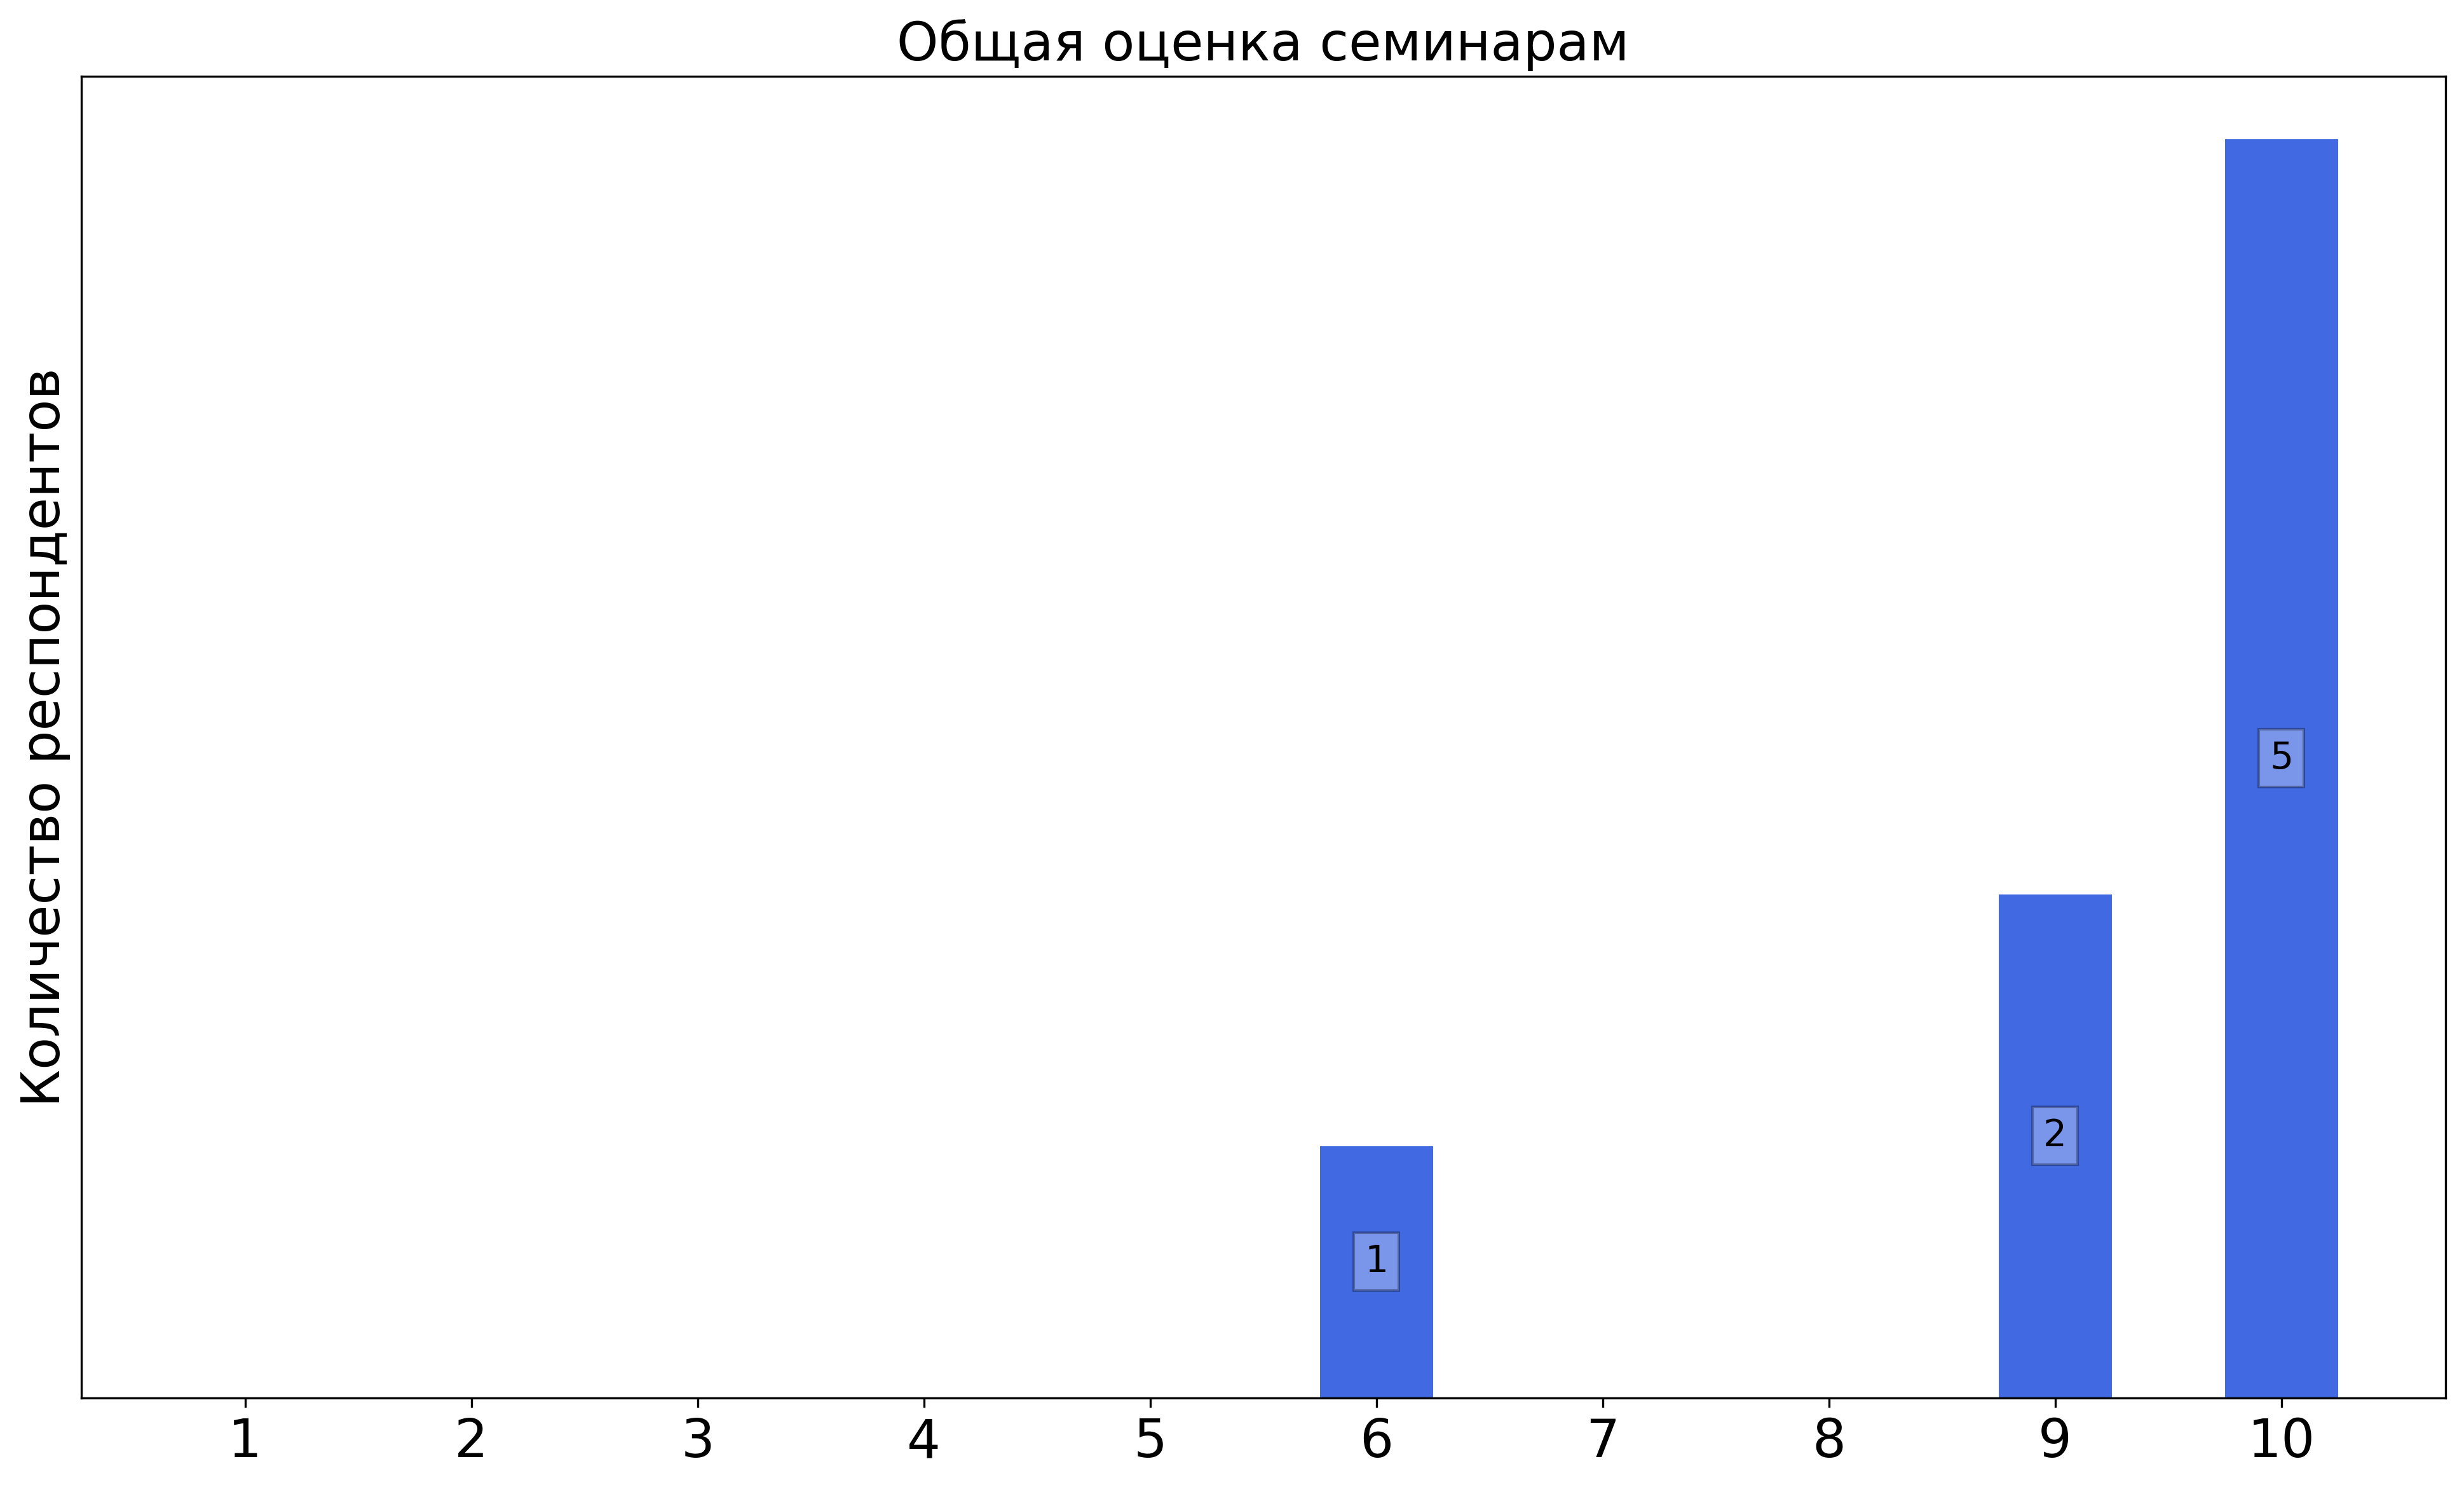
\includegraphics[width=\textwidth]{images/3 course/Общая физика - квантовая физика/seminarists-marks-Кубышкин А.В.-3.png}
                \end{subfigure}	
                \caption{Оценки респондентов о качестве преподавания семинаров}
            \end{figure}

            \textbf{Комментарии студентов о семинаристе\protect\footnote{сохранены оригинальные орфография и пунктуация}}
                \begin{commentbox} 
                    Мега топовый практик, хорошо объясняет, дает материалы по подготовке к госу 
                \end{commentbox} 
            
                \begin{commentbox} 
                    Человек, знающий своё дело. Объясняет очень хорошо.  
                \end{commentbox} 
            
                \begin{commentbox} 
                    В целом, нормально, не всегда было понятно, но проблема может быть в том, что я сам в семестре не очень активно ботал квантфиз. Но семинары всегда проходили бодро. Сдавали задания понедельно. В начале каждого семинара можно было взять доп задачу/вопрос (идейные чаще всего) по прошлой неделе, что влияло на отл. Я всегда их брал, решать вопрос можно было в течение всего семинара 
                \end{commentbox} 
            
                \begin{commentbox} 
                    Повторяет разбор задач из Овчинкина и Корявова, при этом иногда морозит ересь. Расшарить физику не помогает, но справедливо оценивает контрольные и письмак по ГОСу, сдача задания халявная, забавный. 
                \end{commentbox} 
            
                \begin{commentbox} 
                    Замечательный семинарист, на семинарах рассказывал кусок теории нужный для понимания задач. Задания принимал каждую неделю, что максимально снизило нагрузку при сдаче. Контрольные во всех смыслах справедливые, как и оценки за семестр. Всегда готов ответить на вопрос, поддержать, пойти на встречу и даже поднять оценку за контрольные дополнительными задачами.  
                \end{commentbox} 
        

        \subsubsection{Отзыв студентов о семинарах. Семинарист: Лапушкин Г.И.}
            \begin{figure}[H]
                \centering
                \begin{subfigure}[b]{0.45\textwidth}
                    \centering
                    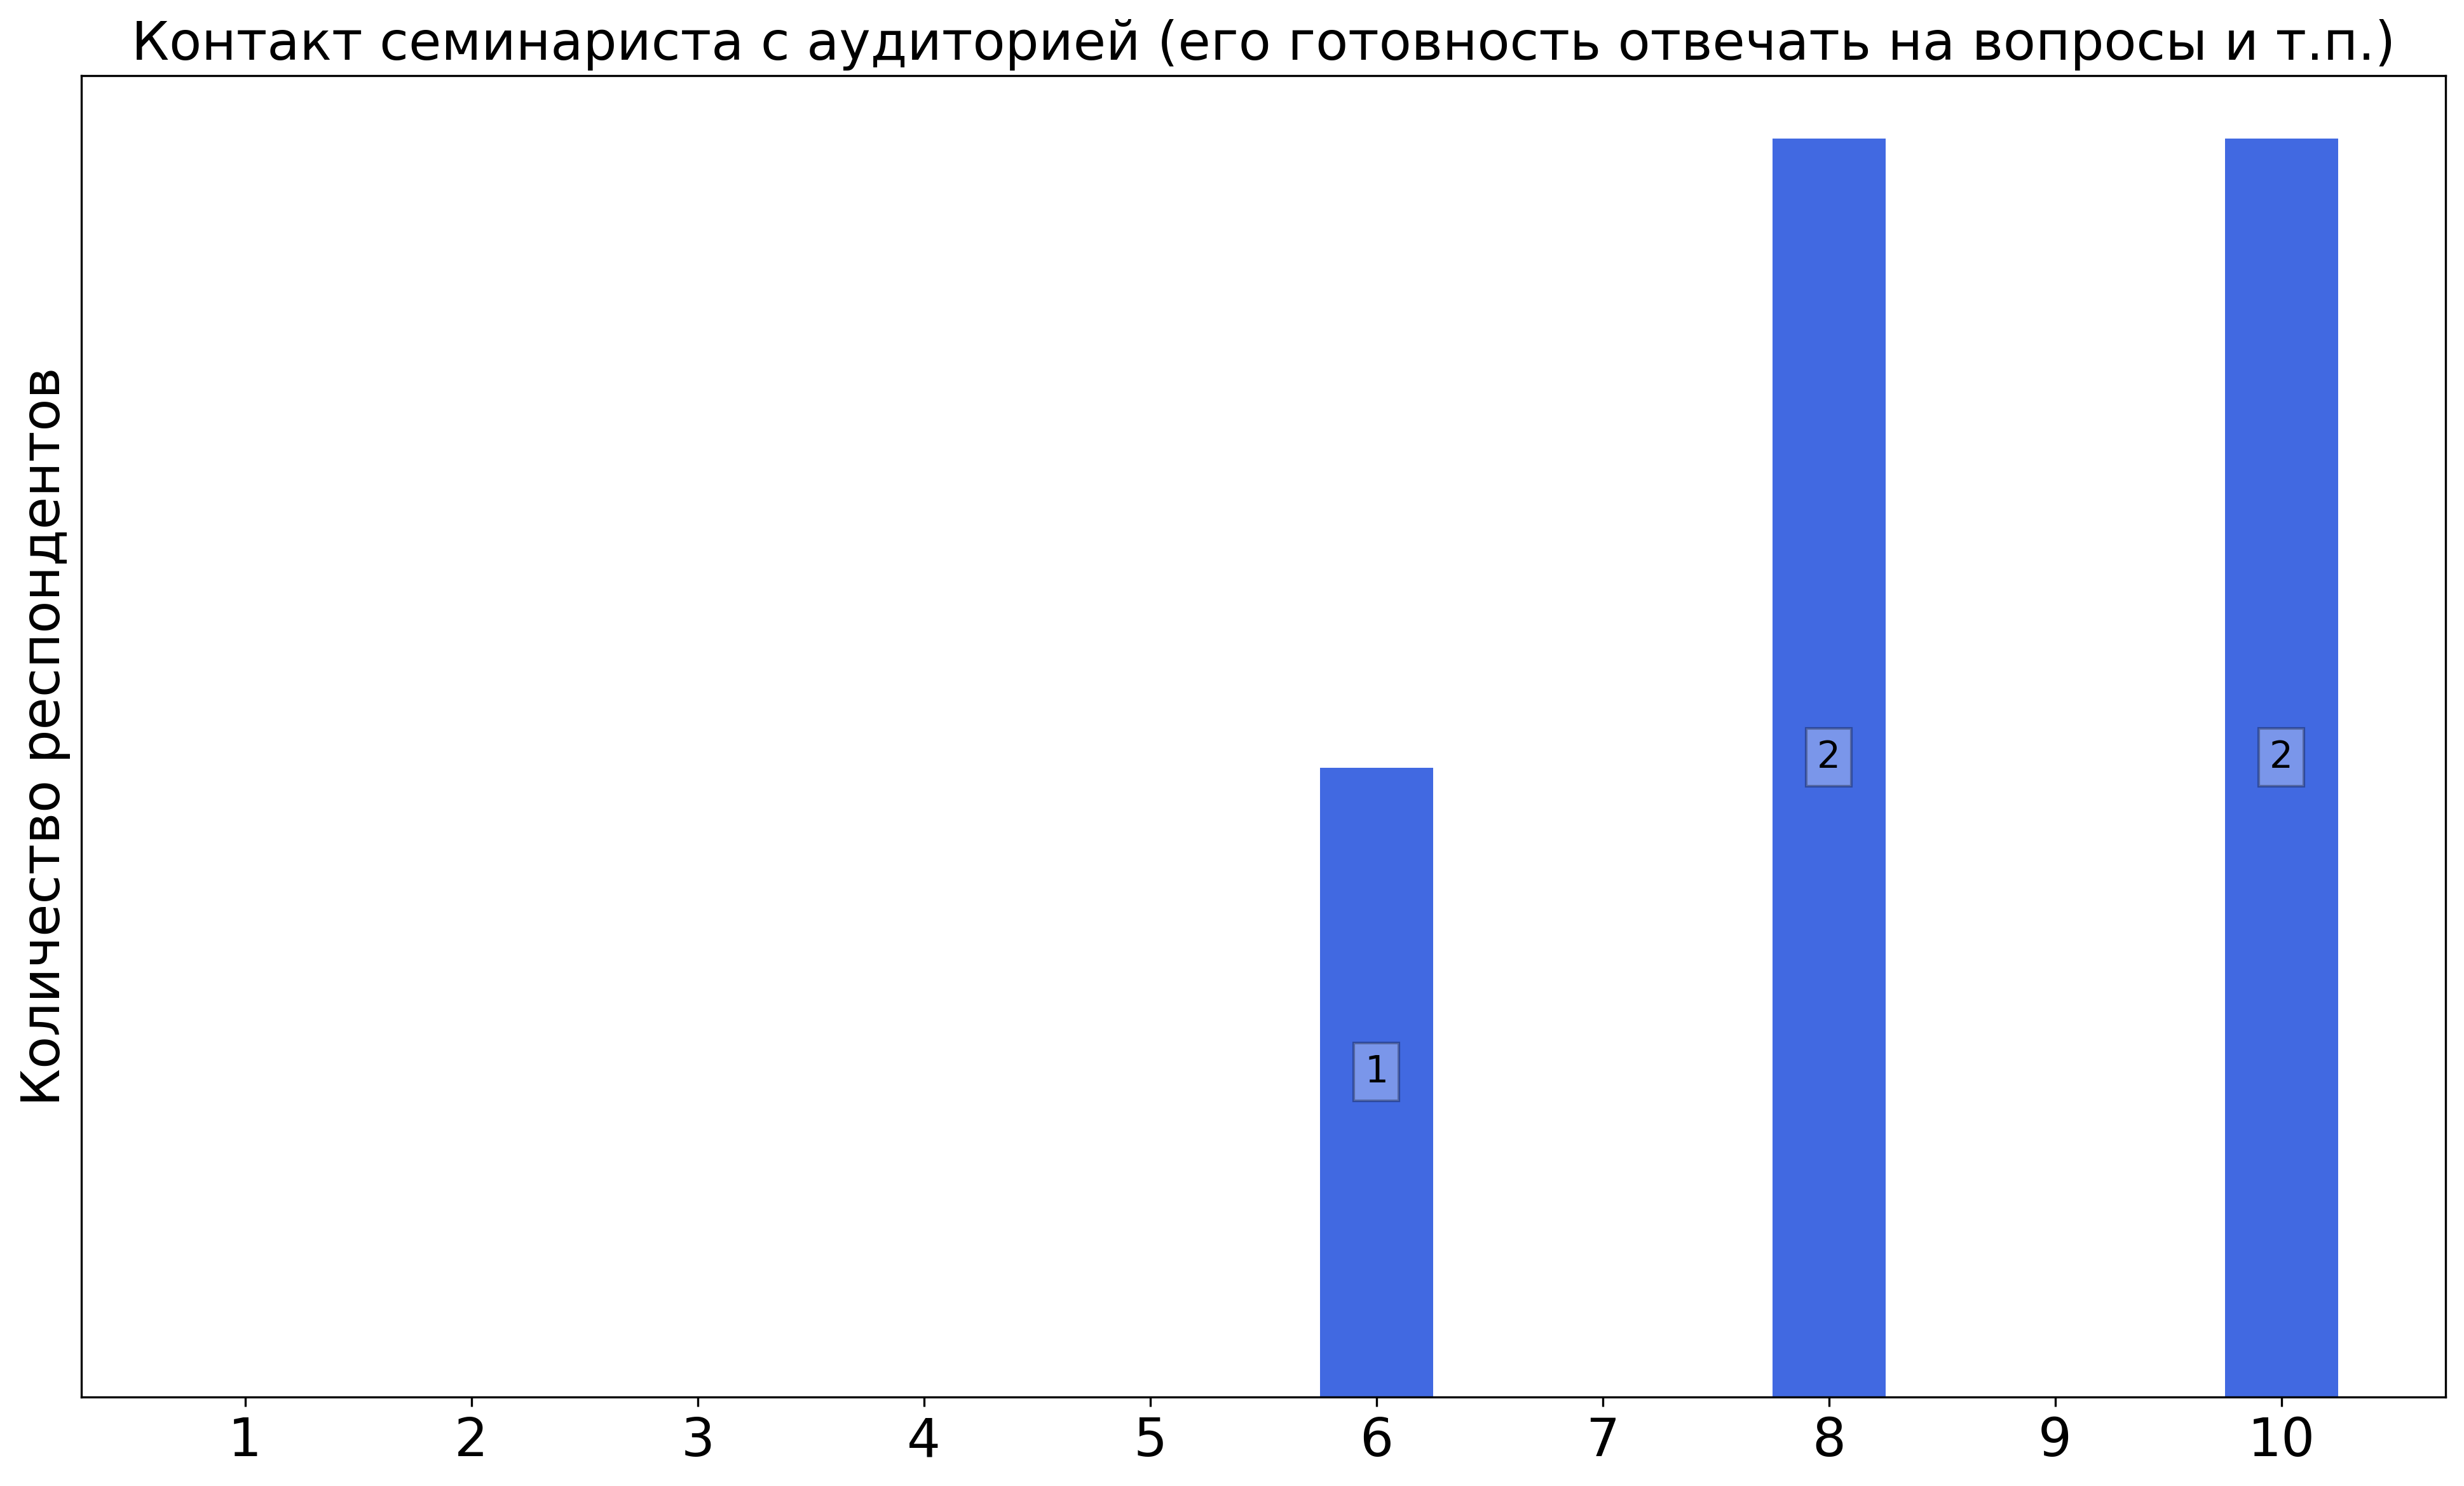
\includegraphics[width=\textwidth]{images/3 course/Общая физика - квантовая физика/seminarists-marks-Лапушкин Г.И.-0.png}
                \end{subfigure}
                \begin{subfigure}[b]{0.45\textwidth}
                    \centering
                    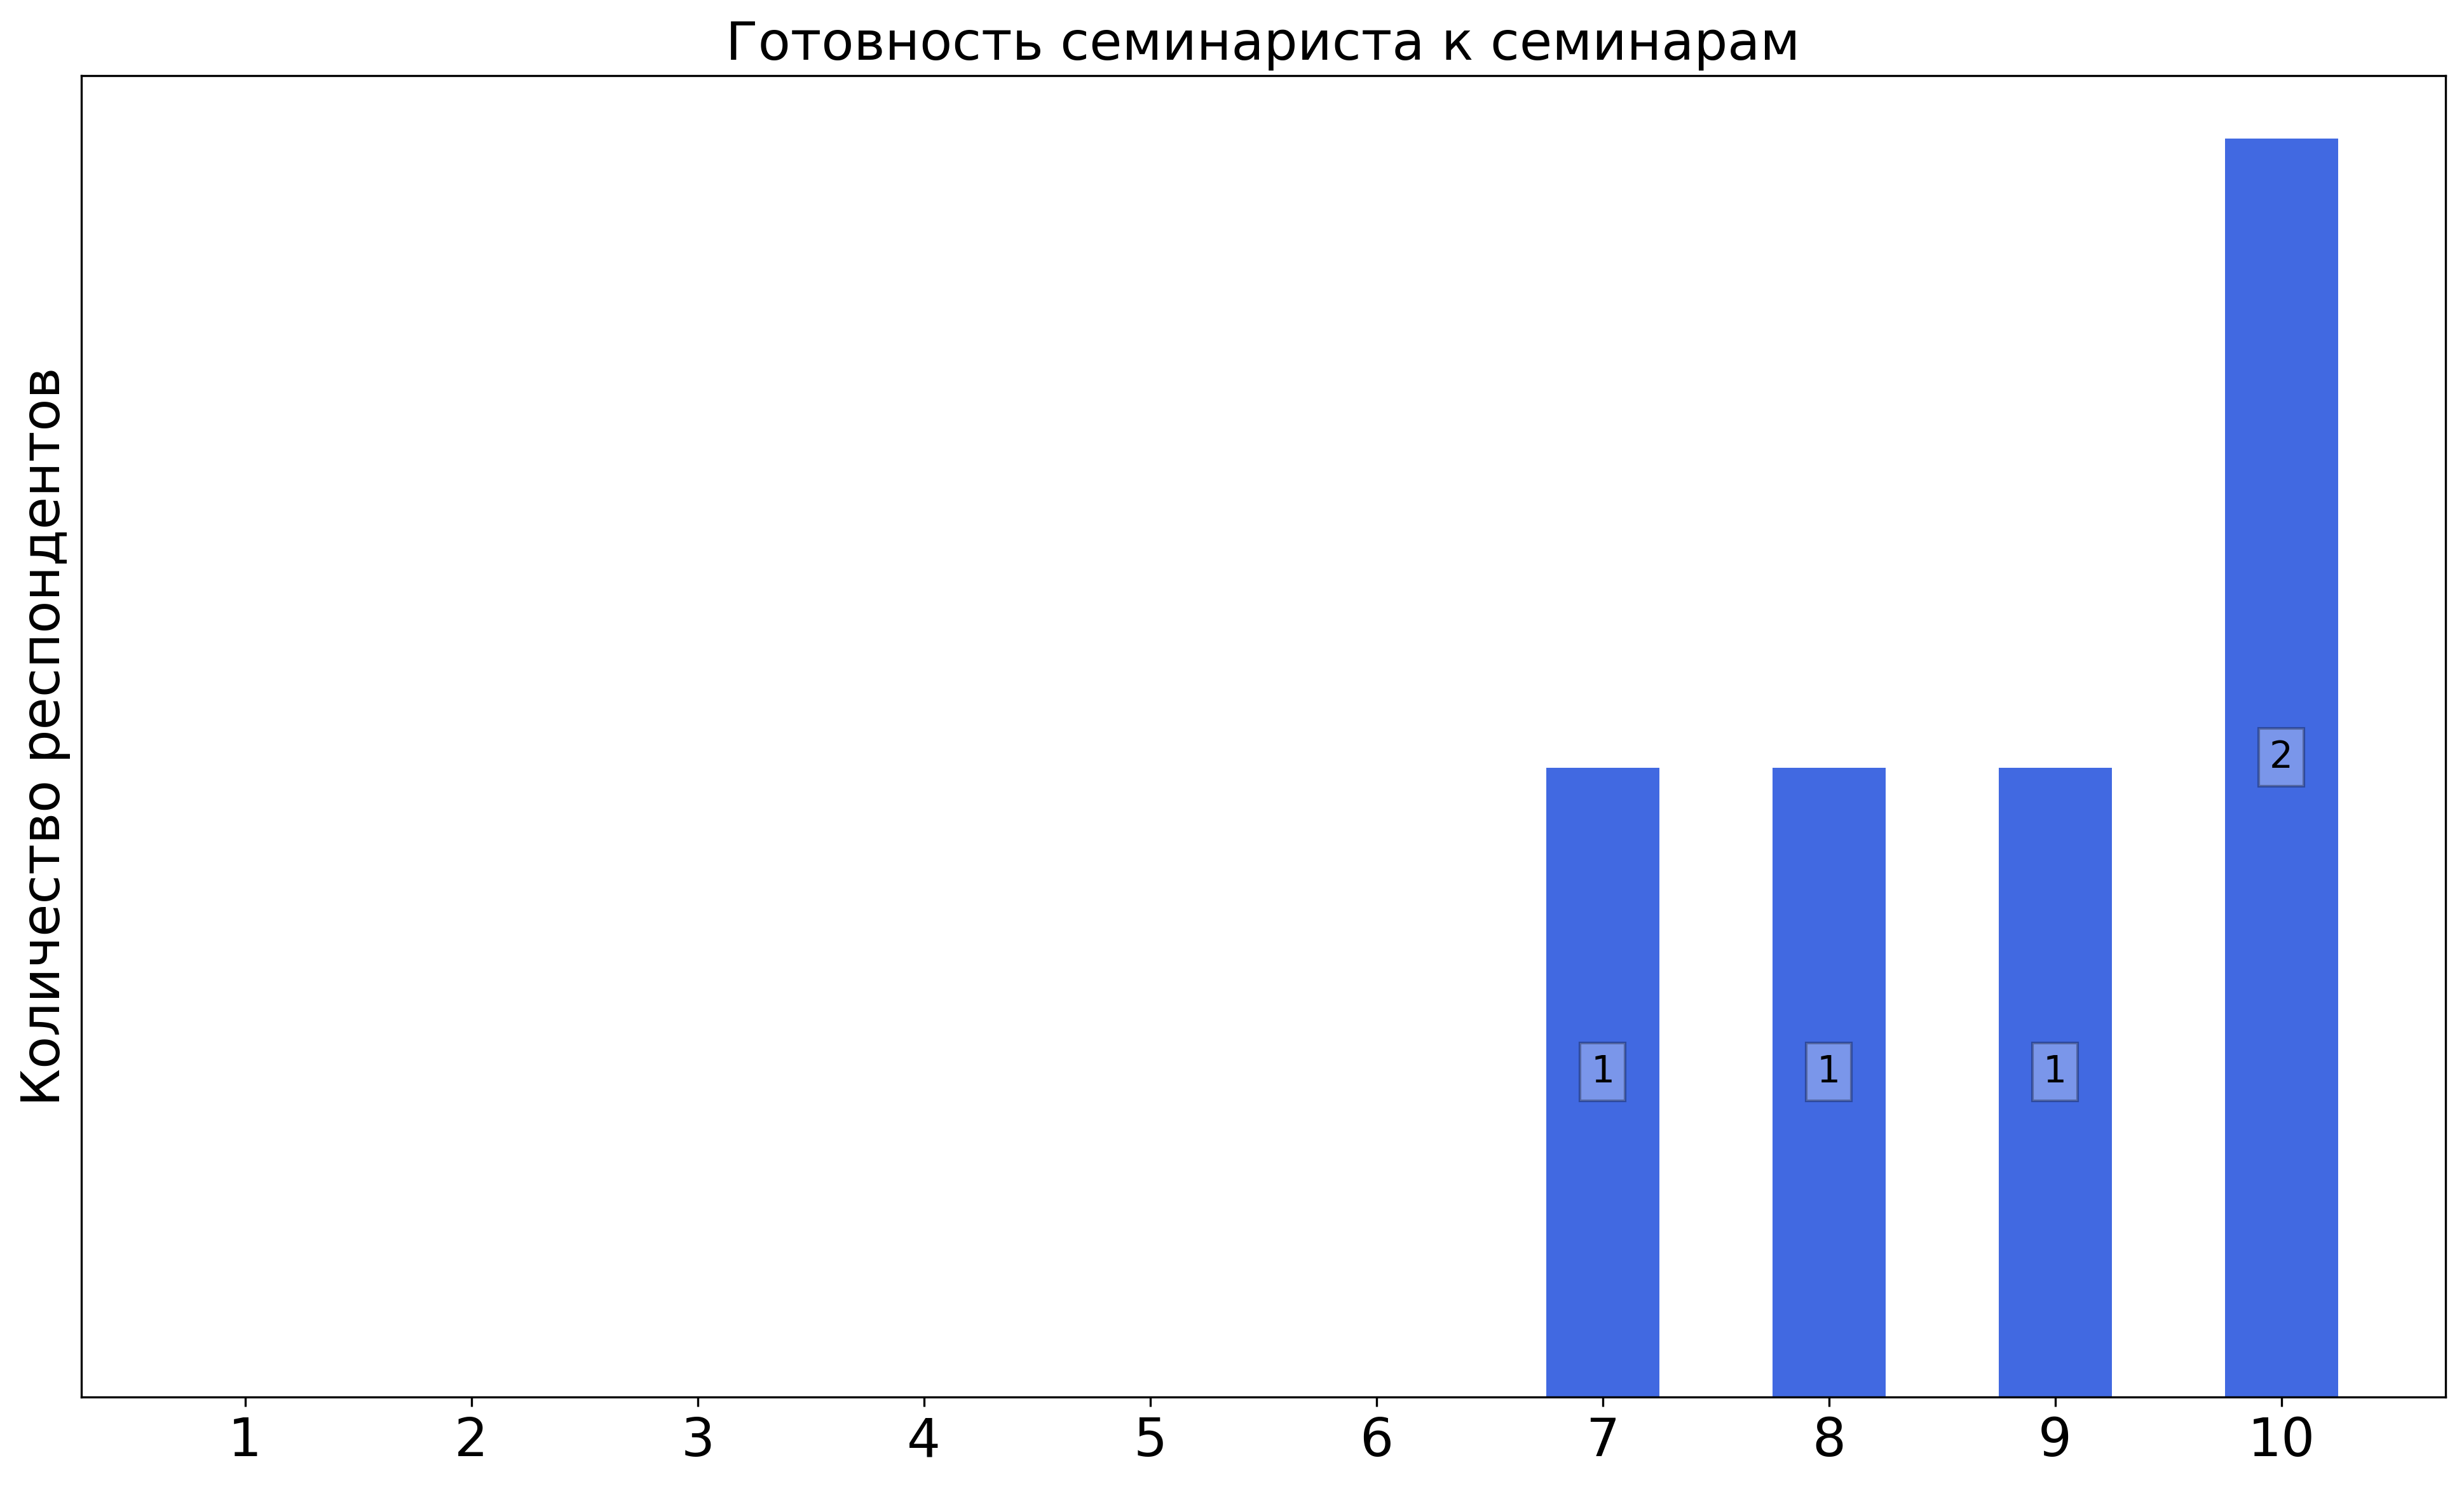
\includegraphics[width=\textwidth]{images/3 course/Общая физика - квантовая физика/seminarists-marks-Лапушкин Г.И.-1.png}
                \end{subfigure}
                \begin{subfigure}[b]{0.45\textwidth}
                    \centering
                    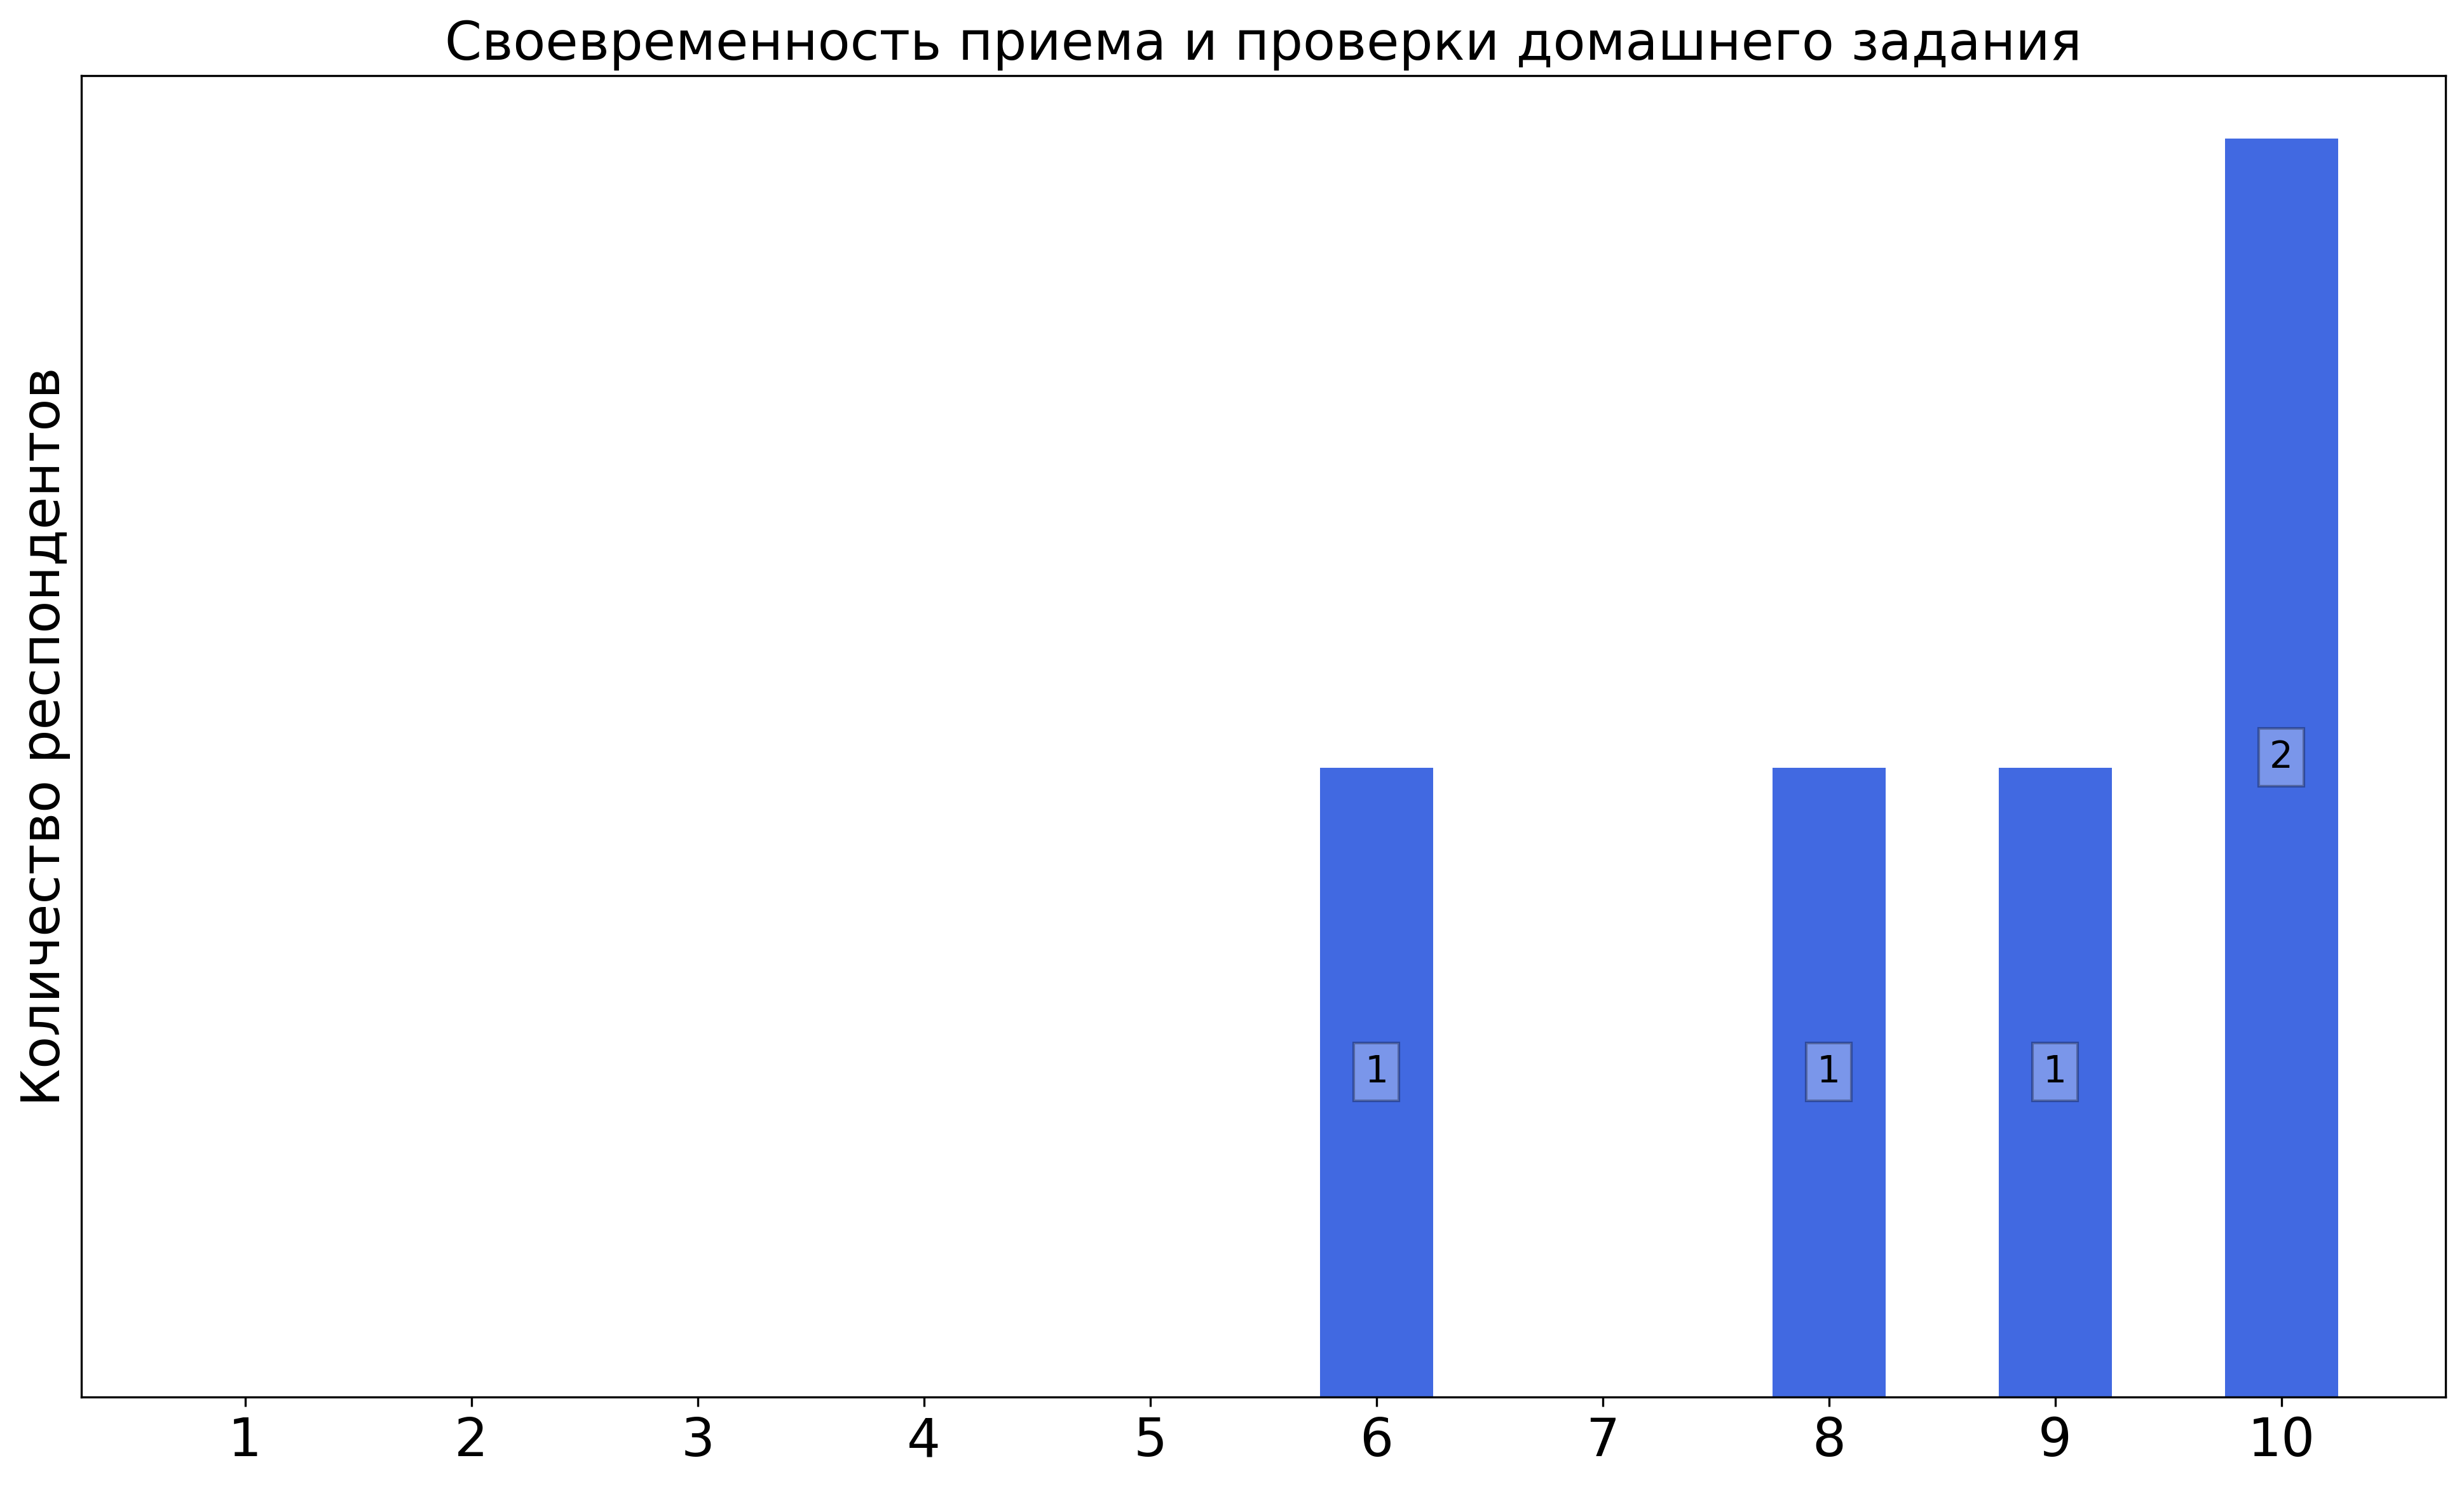
\includegraphics[width=\textwidth]{images/3 course/Общая физика - квантовая физика/seminarists-marks-Лапушкин Г.И.-2.png}
                \end{subfigure}
                \begin{subfigure}[b]{0.45\textwidth}
                    \centering
                    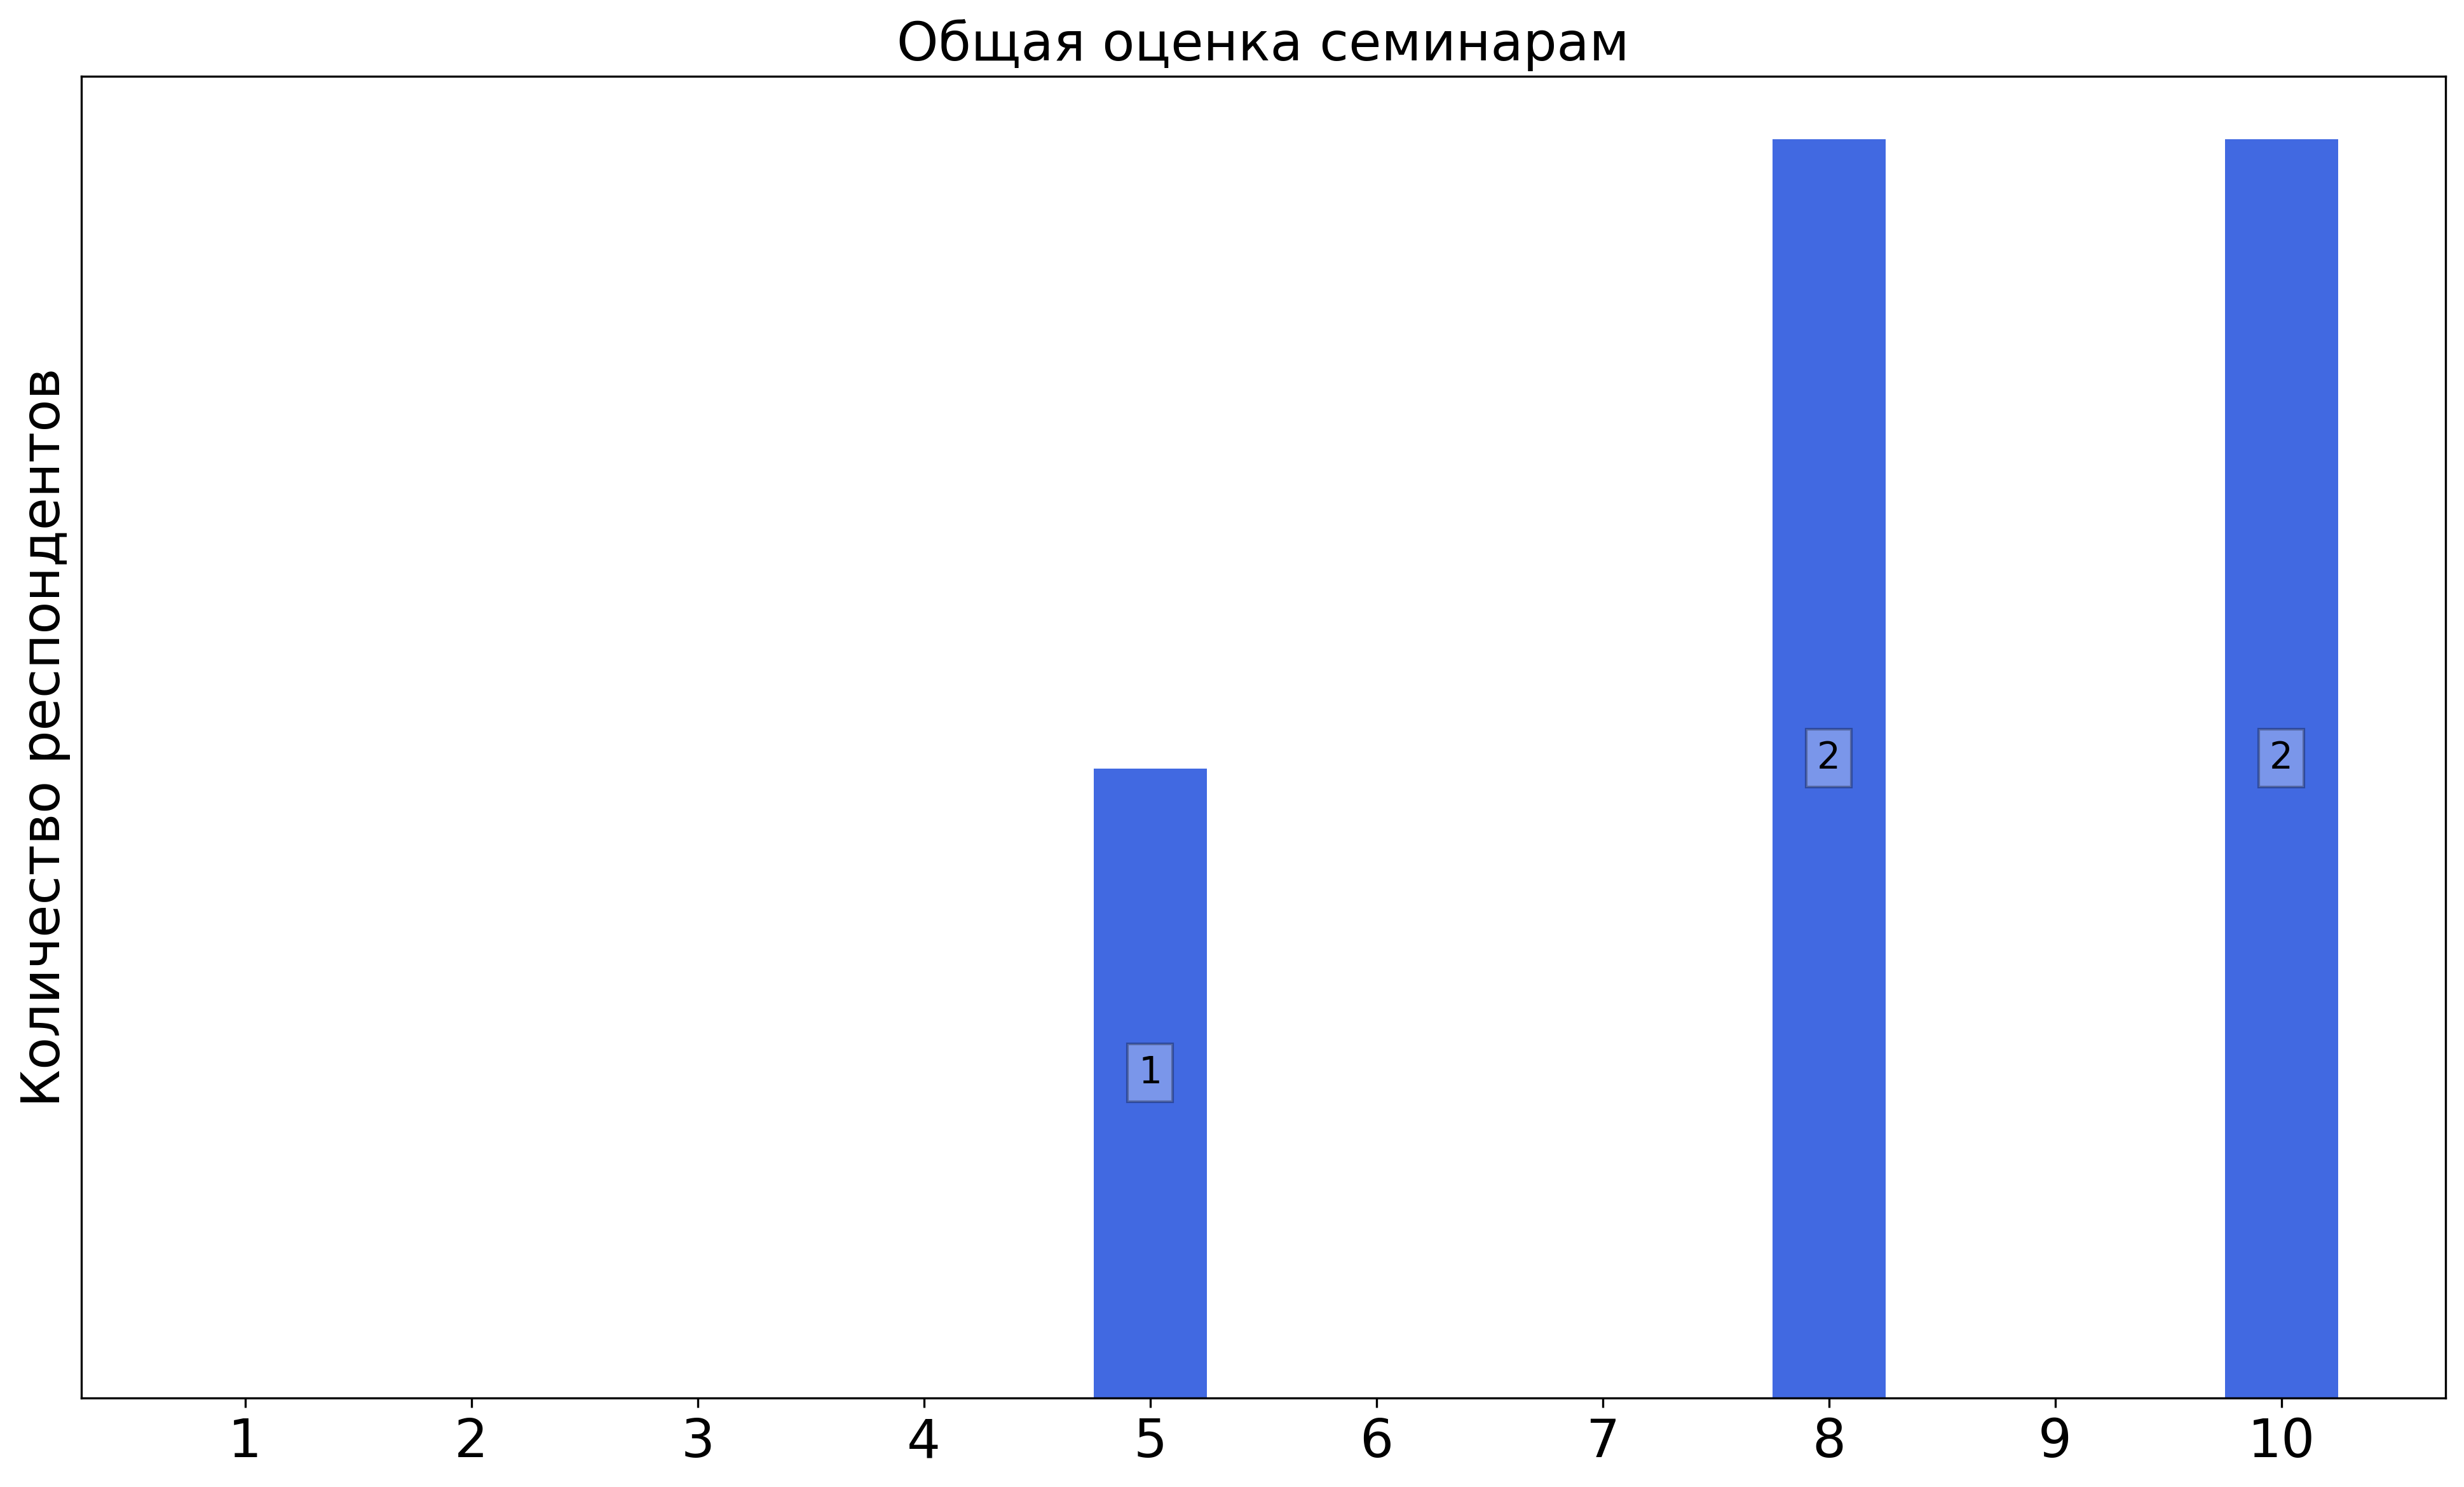
\includegraphics[width=\textwidth]{images/3 course/Общая физика - квантовая физика/seminarists-marks-Лапушкин Г.И.-3.png}
                \end{subfigure}	
                \caption{Оценки респондентов о качестве преподавания семинаров}
            \end{figure}

            \textbf{Комментарии студентов о семинаристе\protect\footnote{сохранены оригинальные орфография и пунктуация}}
                \begin{commentbox} 
                    Как преподаватель хороший, объясняет понятно, слишком много не требует
                    Иногда достает тем, что говорит "вы не сдадите гос, не напишите кр" и тд 
                \end{commentbox} 
        

        \subsubsection{Отзыв студентов о семинарах. Семинарист: Овчинкин В.А.}
            \begin{figure}[H]
                \centering
                \begin{subfigure}[b]{0.45\textwidth}
                    \centering
                    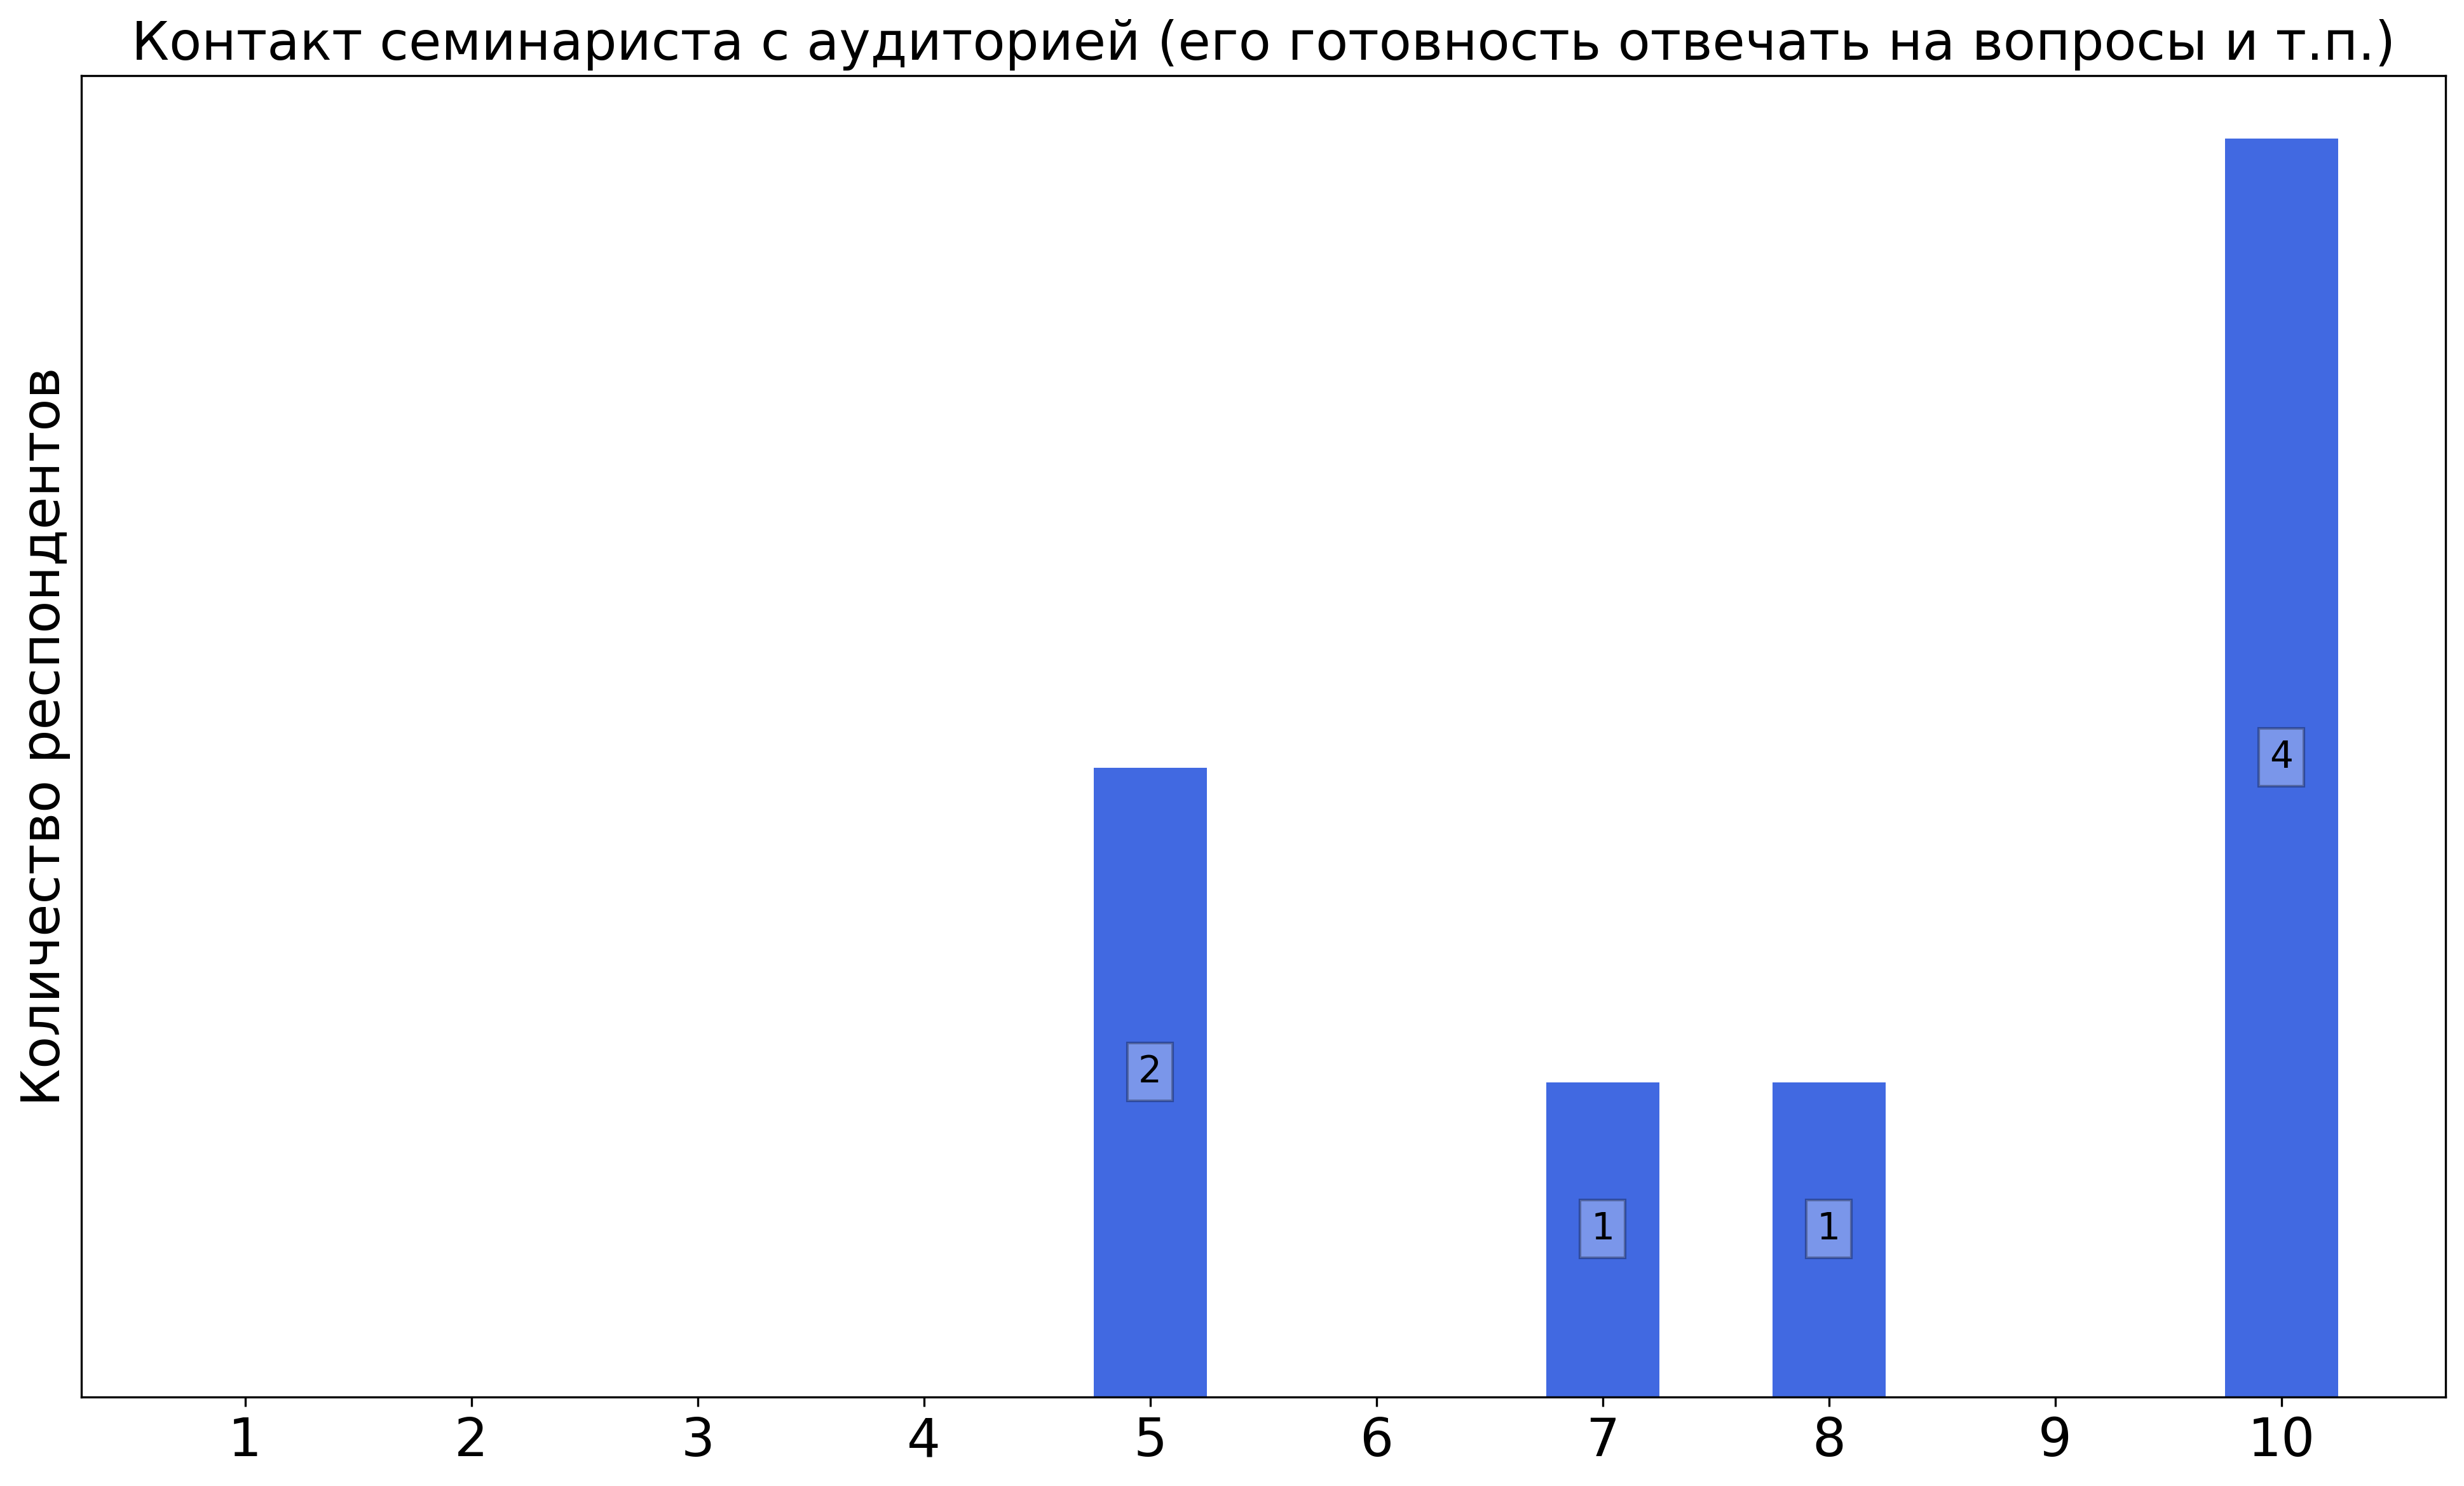
\includegraphics[width=\textwidth]{images/3 course/Общая физика - квантовая физика/seminarists-marks-Овчинкин В.А.-0.png}
                \end{subfigure}
                \begin{subfigure}[b]{0.45\textwidth}
                    \centering
                    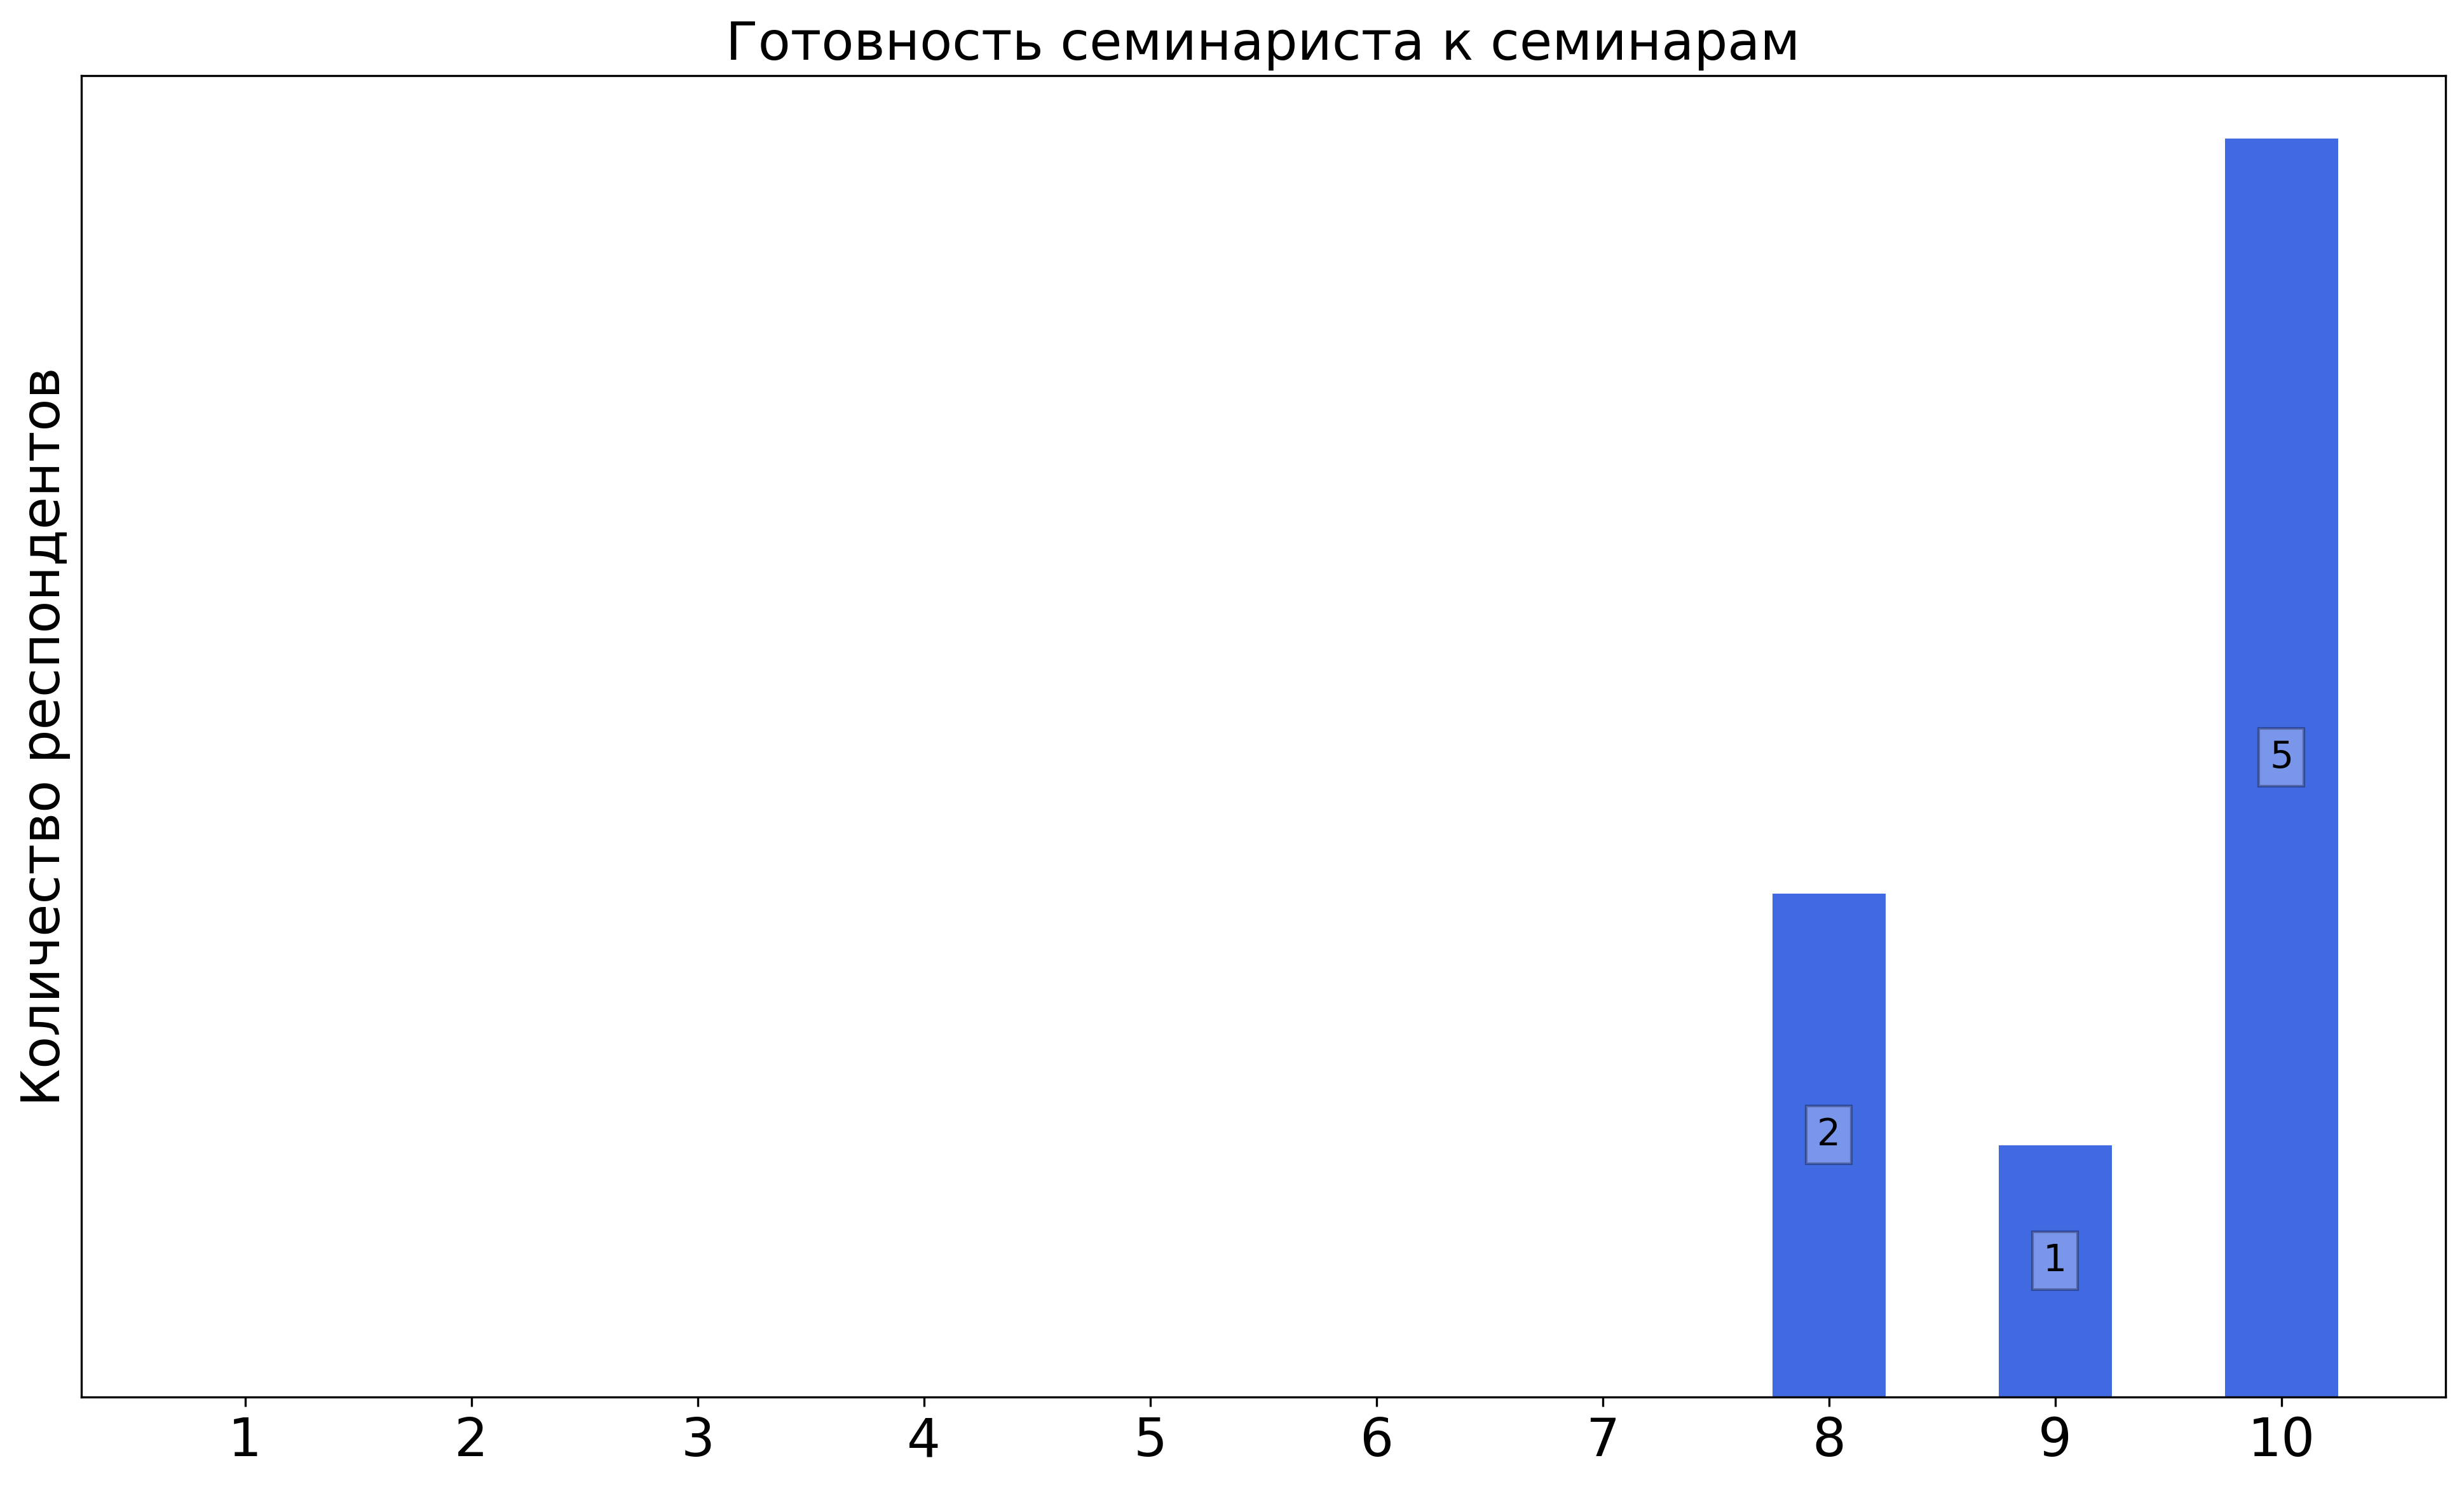
\includegraphics[width=\textwidth]{images/3 course/Общая физика - квантовая физика/seminarists-marks-Овчинкин В.А.-1.png}
                \end{subfigure}
                \begin{subfigure}[b]{0.45\textwidth}
                    \centering
                    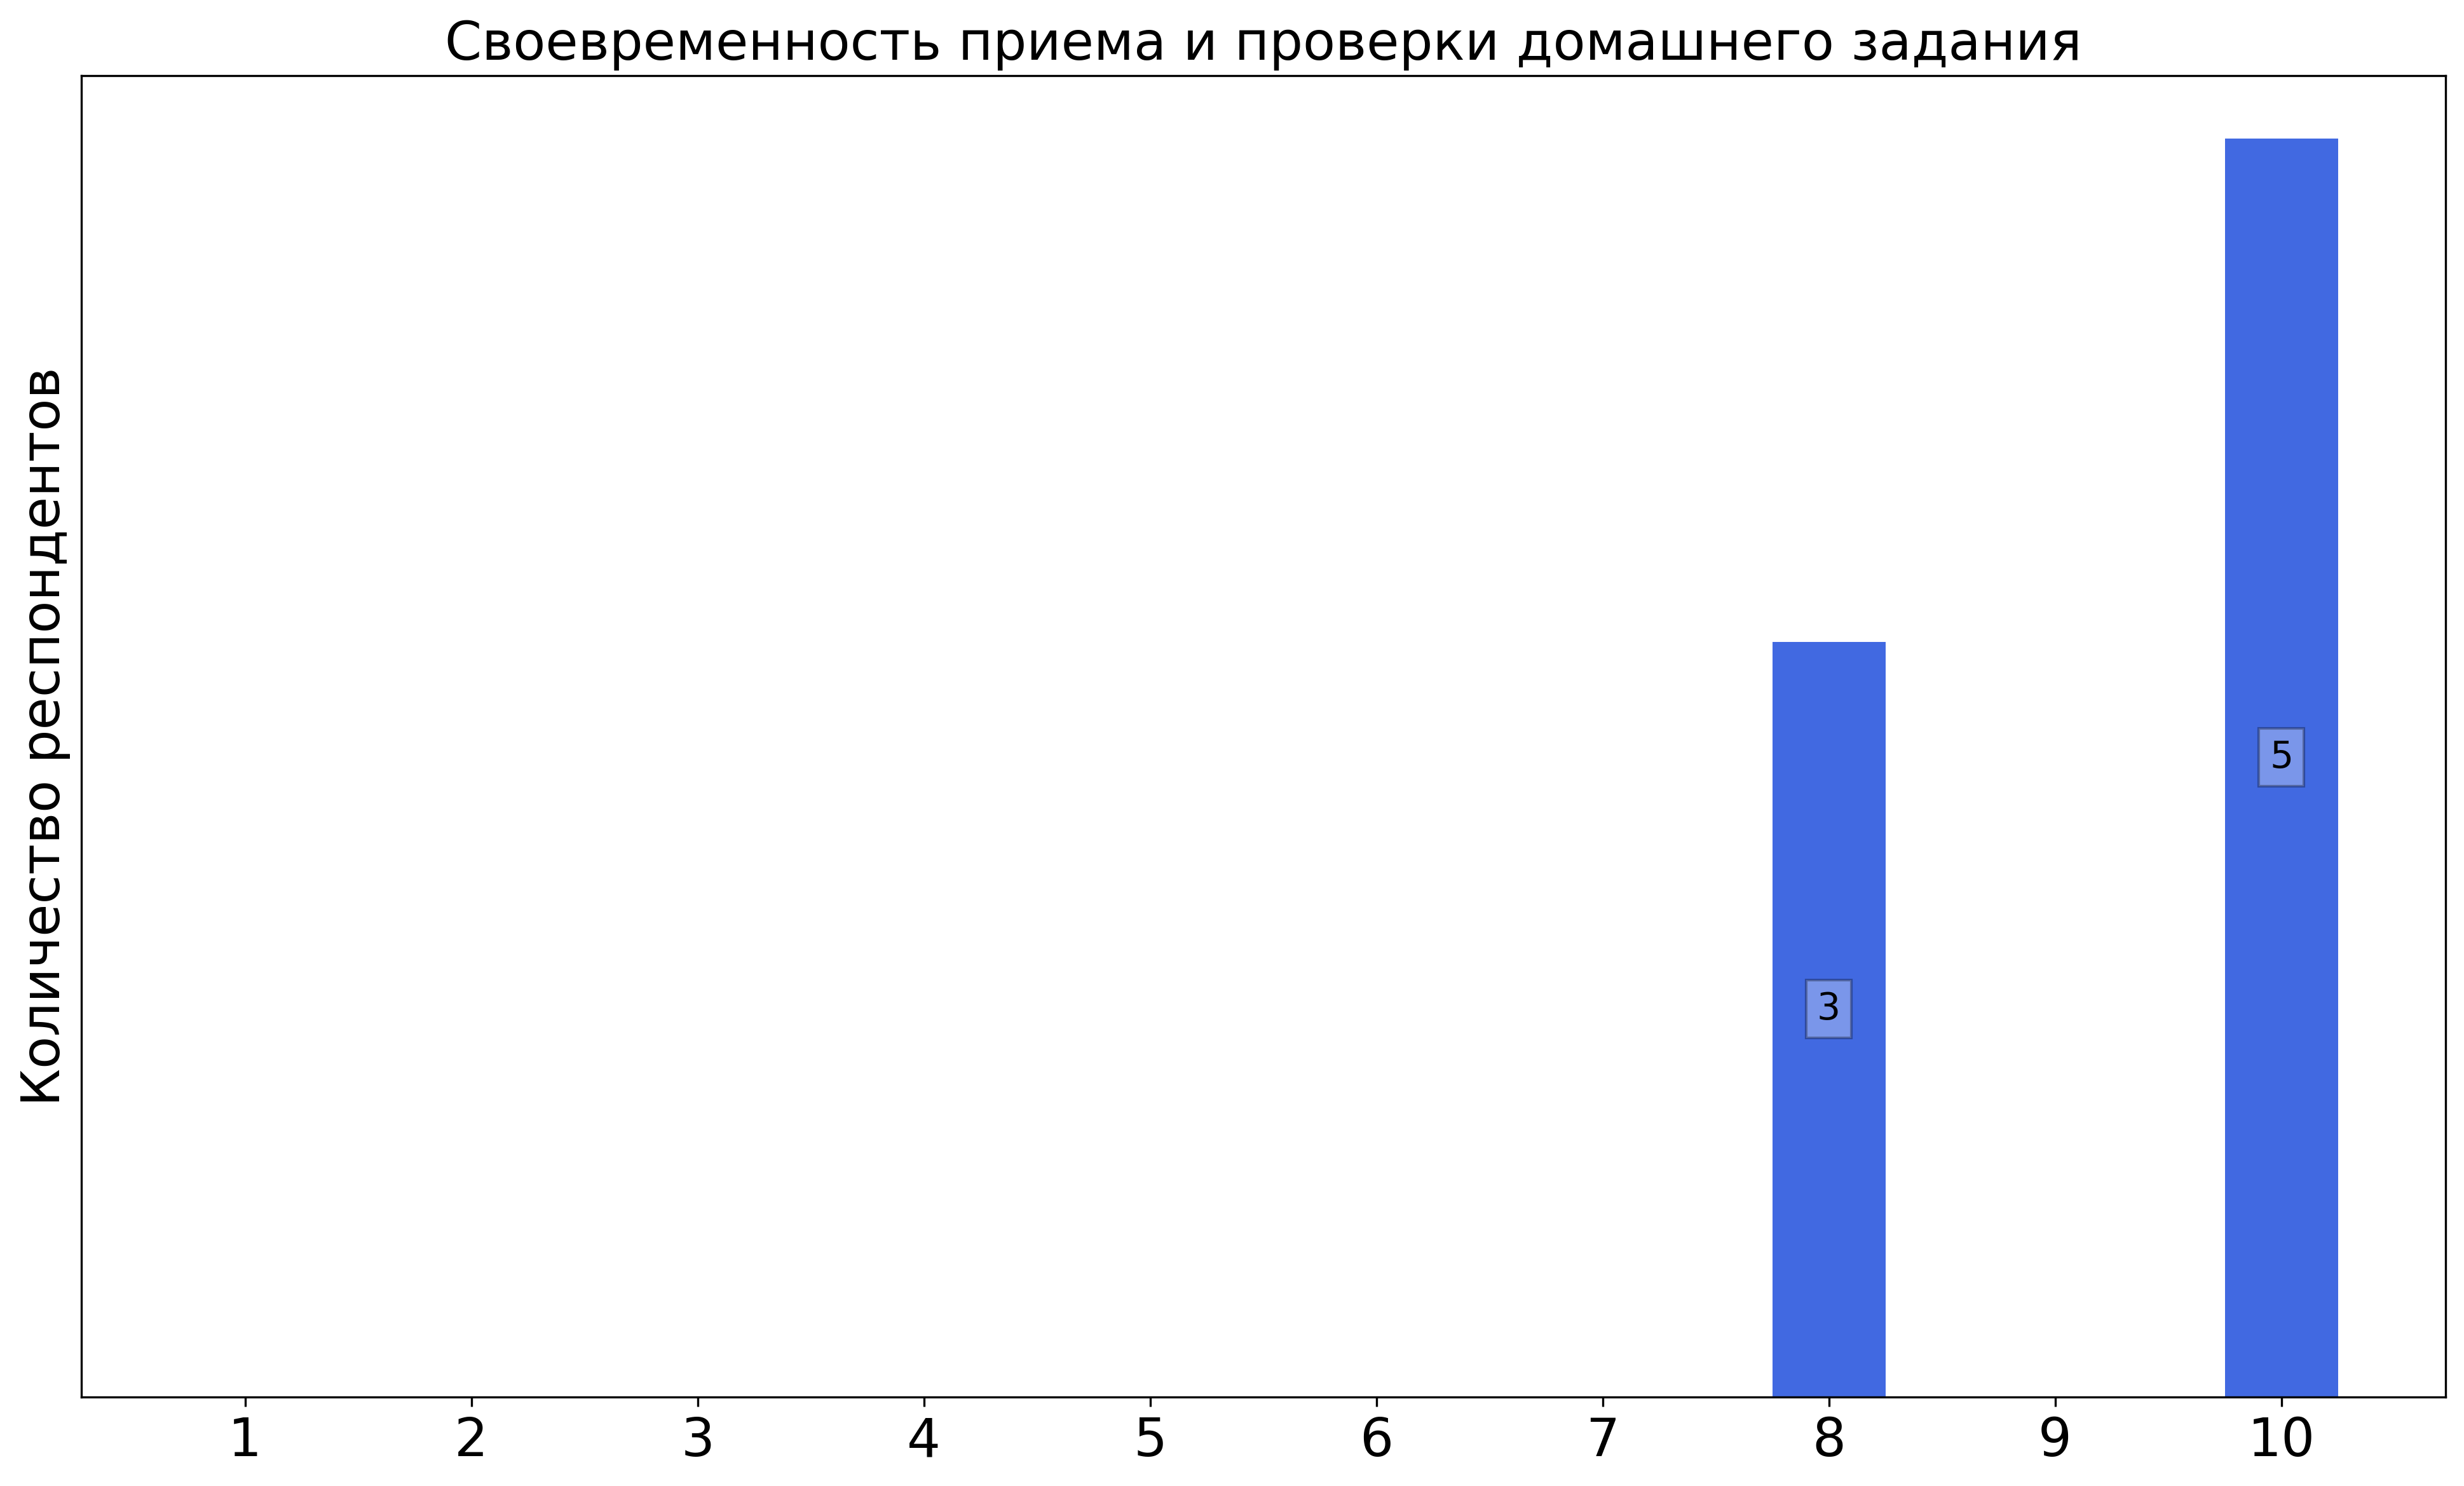
\includegraphics[width=\textwidth]{images/3 course/Общая физика - квантовая физика/seminarists-marks-Овчинкин В.А.-2.png}
                \end{subfigure}
                \begin{subfigure}[b]{0.45\textwidth}
                    \centering
                    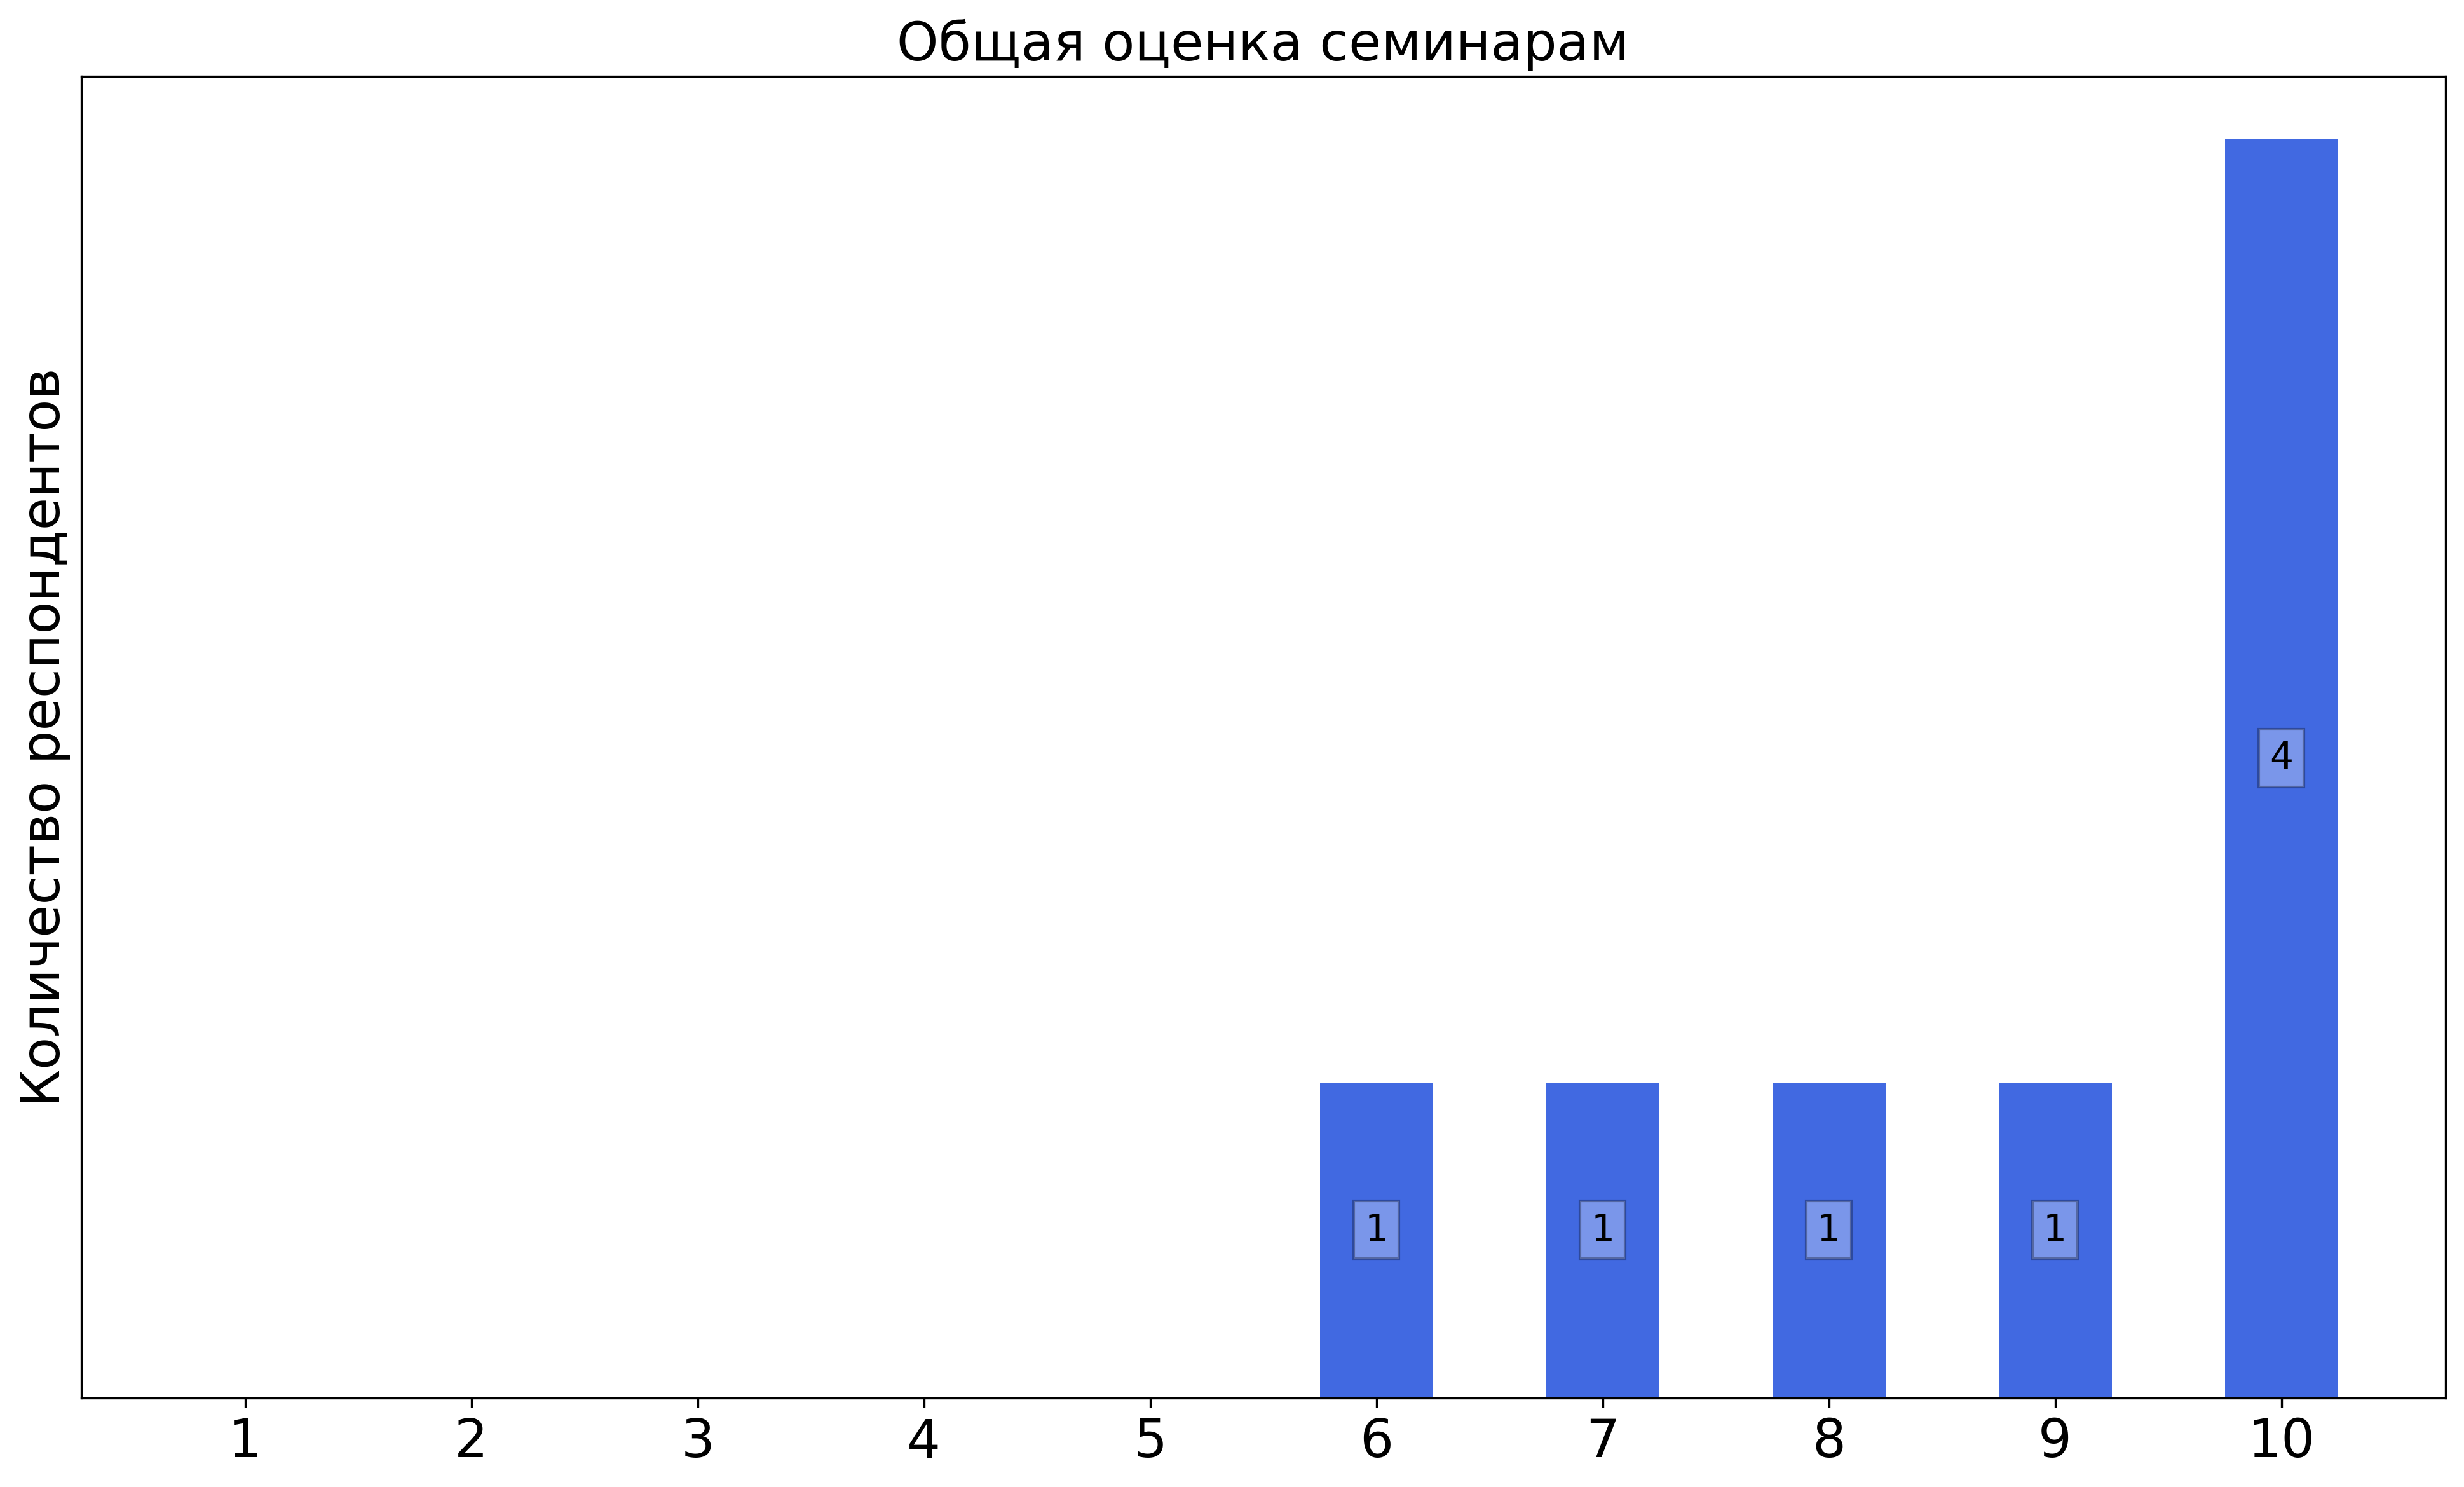
\includegraphics[width=\textwidth]{images/3 course/Общая физика - квантовая физика/seminarists-marks-Овчинкин В.А.-3.png}
                \end{subfigure}	
                \caption{Оценки респондентов о качестве преподавания семинаров}
            \end{figure}

            \textbf{Комментарии студентов о семинаристе\protect\footnote{сохранены оригинальные орфография и пунктуация}}
                \begin{commentbox} 
                    Очень благодарен за понятное объяснение материала! Не понравилась только система оценивания семинариста. Выставляемая оценка не редко зависела от отношения семинариста к обучающемуся. Явно заметна тенденция к выставлению более высоких оценок студентам, с которыми преподаватель давно знаком и находится в хороших, близких отношениях. 
                \end{commentbox} 
            
                \begin{commentbox} 
                    К сожалению, из семинаров я мало что понял. Ходил в надежде что семинарист лучше примет дз. 
                \end{commentbox}


        \subsubsection{Отзыв студентов о семинарах. Семинарист: Покотило И.Л.}
            \begin{figure}[H]
                \centering
                \begin{subfigure}[b]{0.45\textwidth}
                    \centering
                    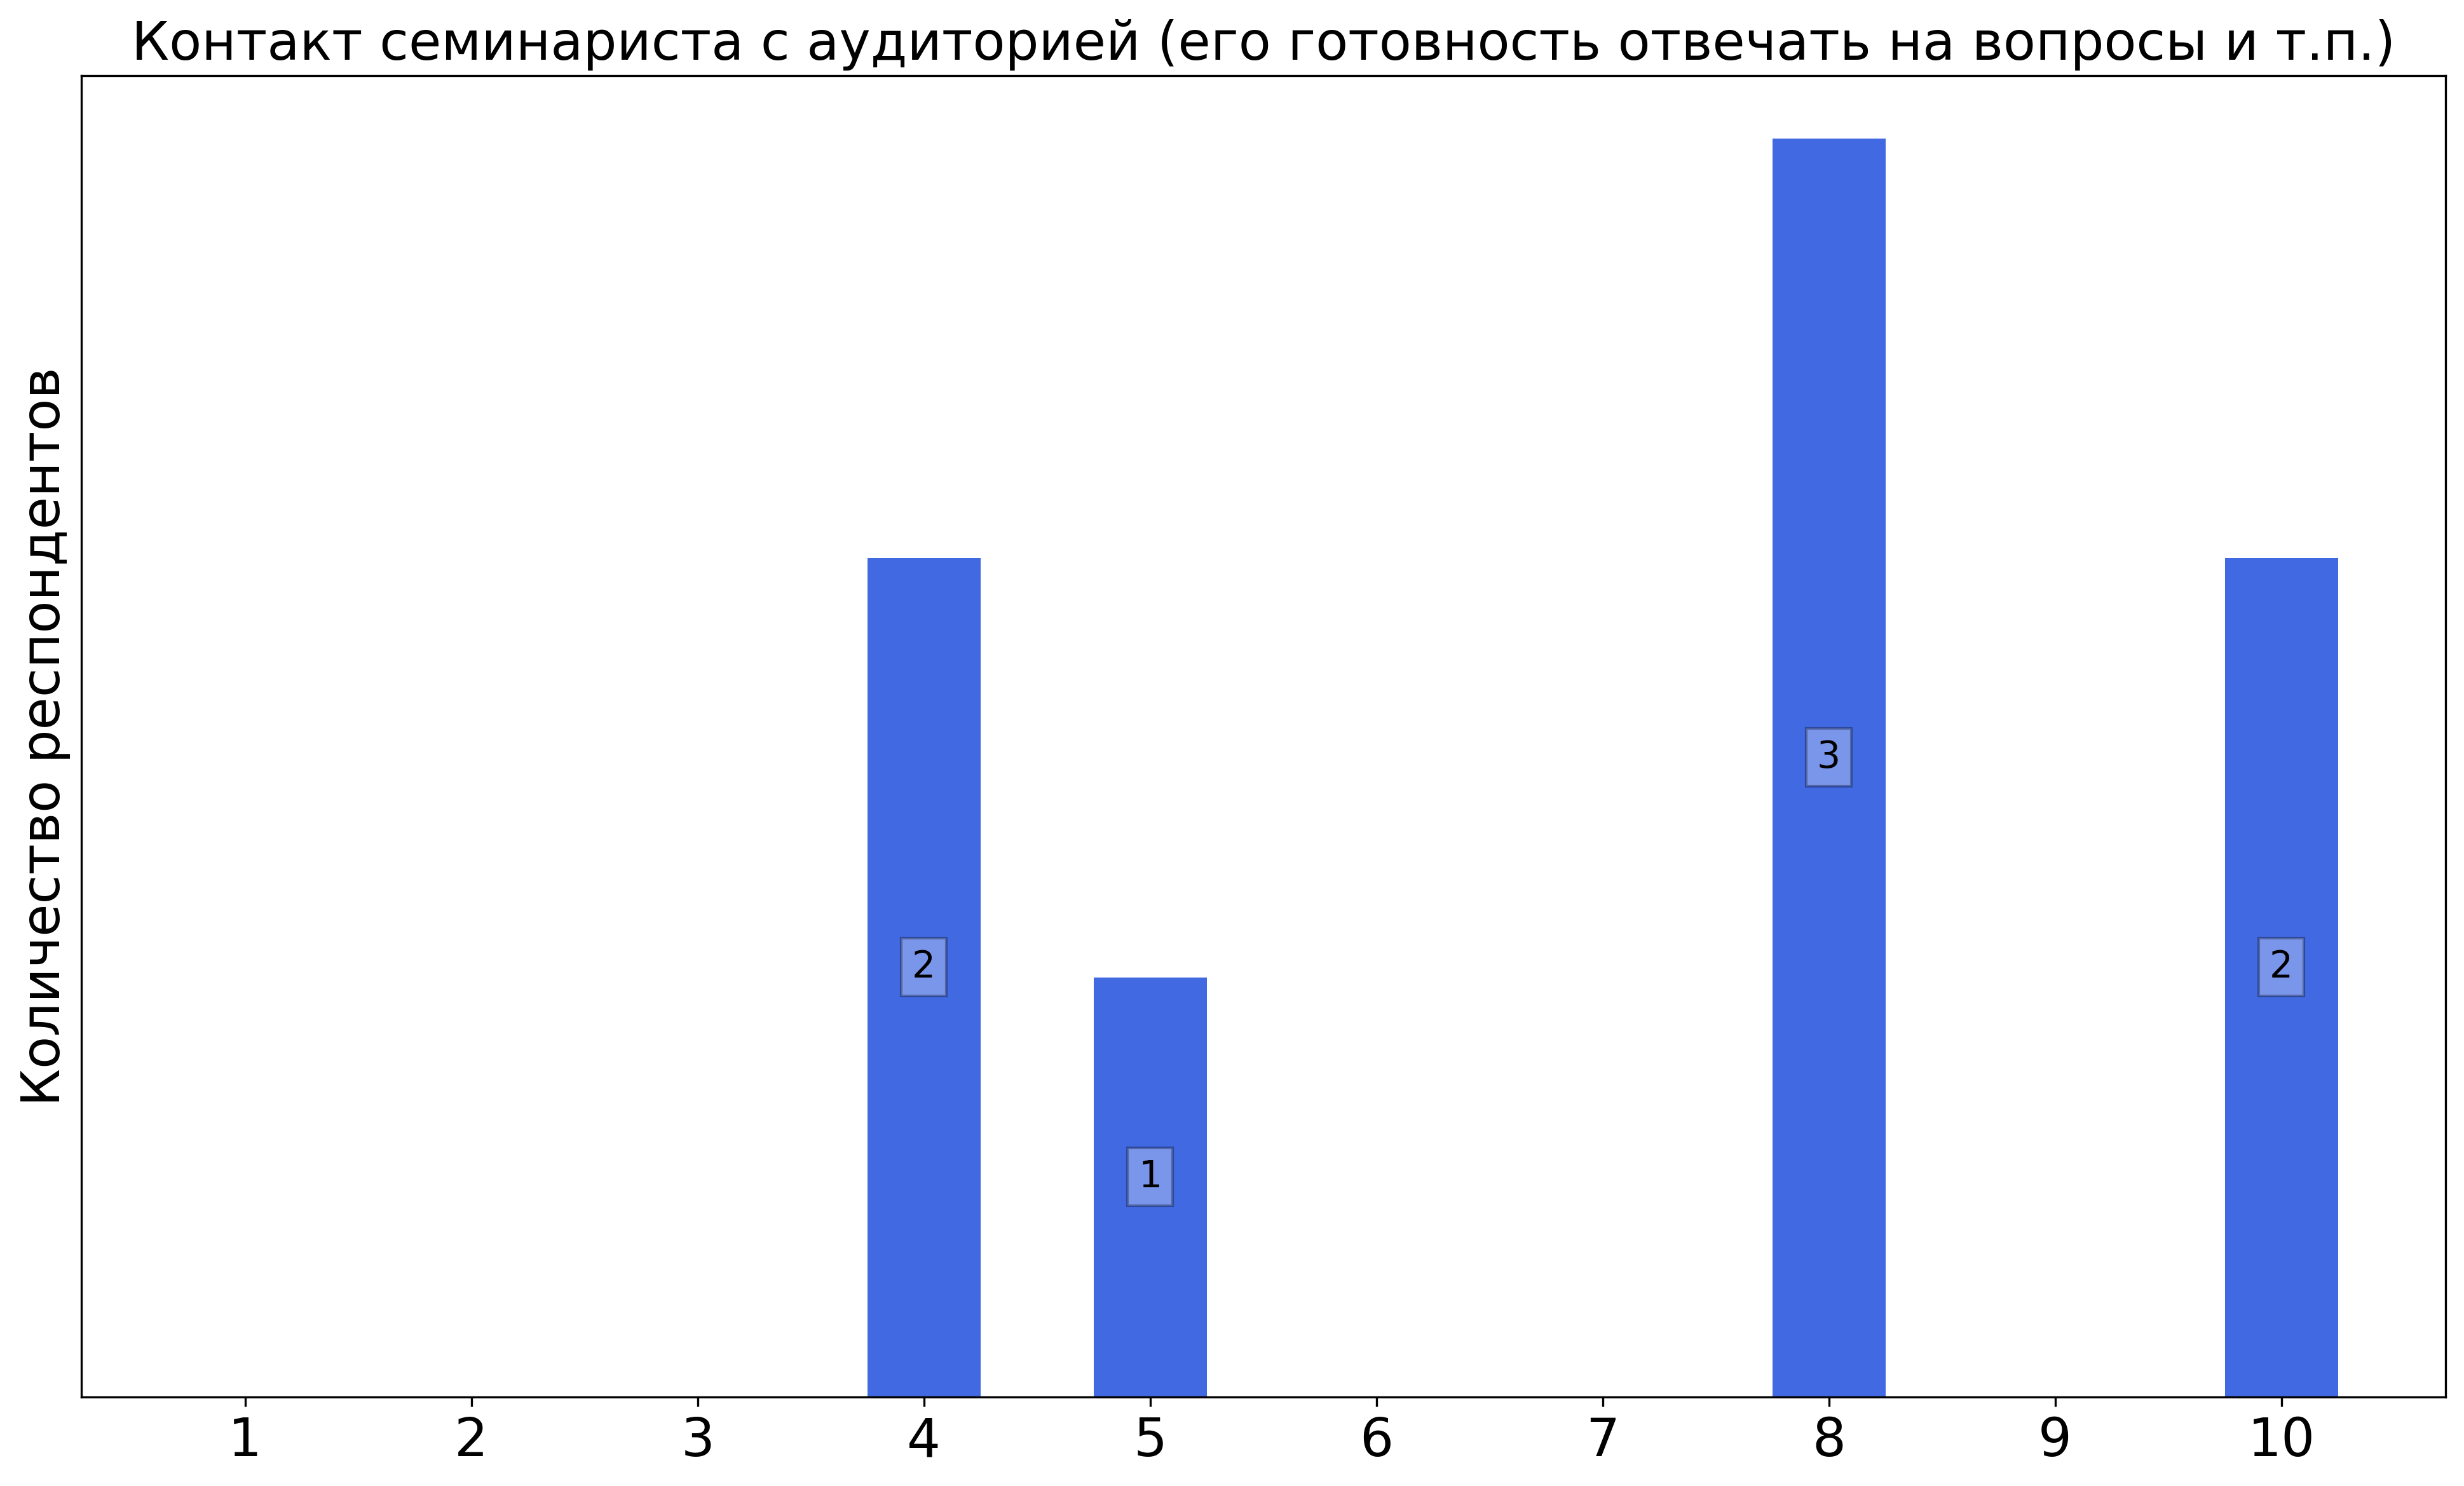
\includegraphics[width=\textwidth]{images/3 course/Общая физика - квантовая физика/seminarists-marks-Покотило И.Л.-0.png}
                \end{subfigure}
                \begin{subfigure}[b]{0.45\textwidth}
                    \centering
                    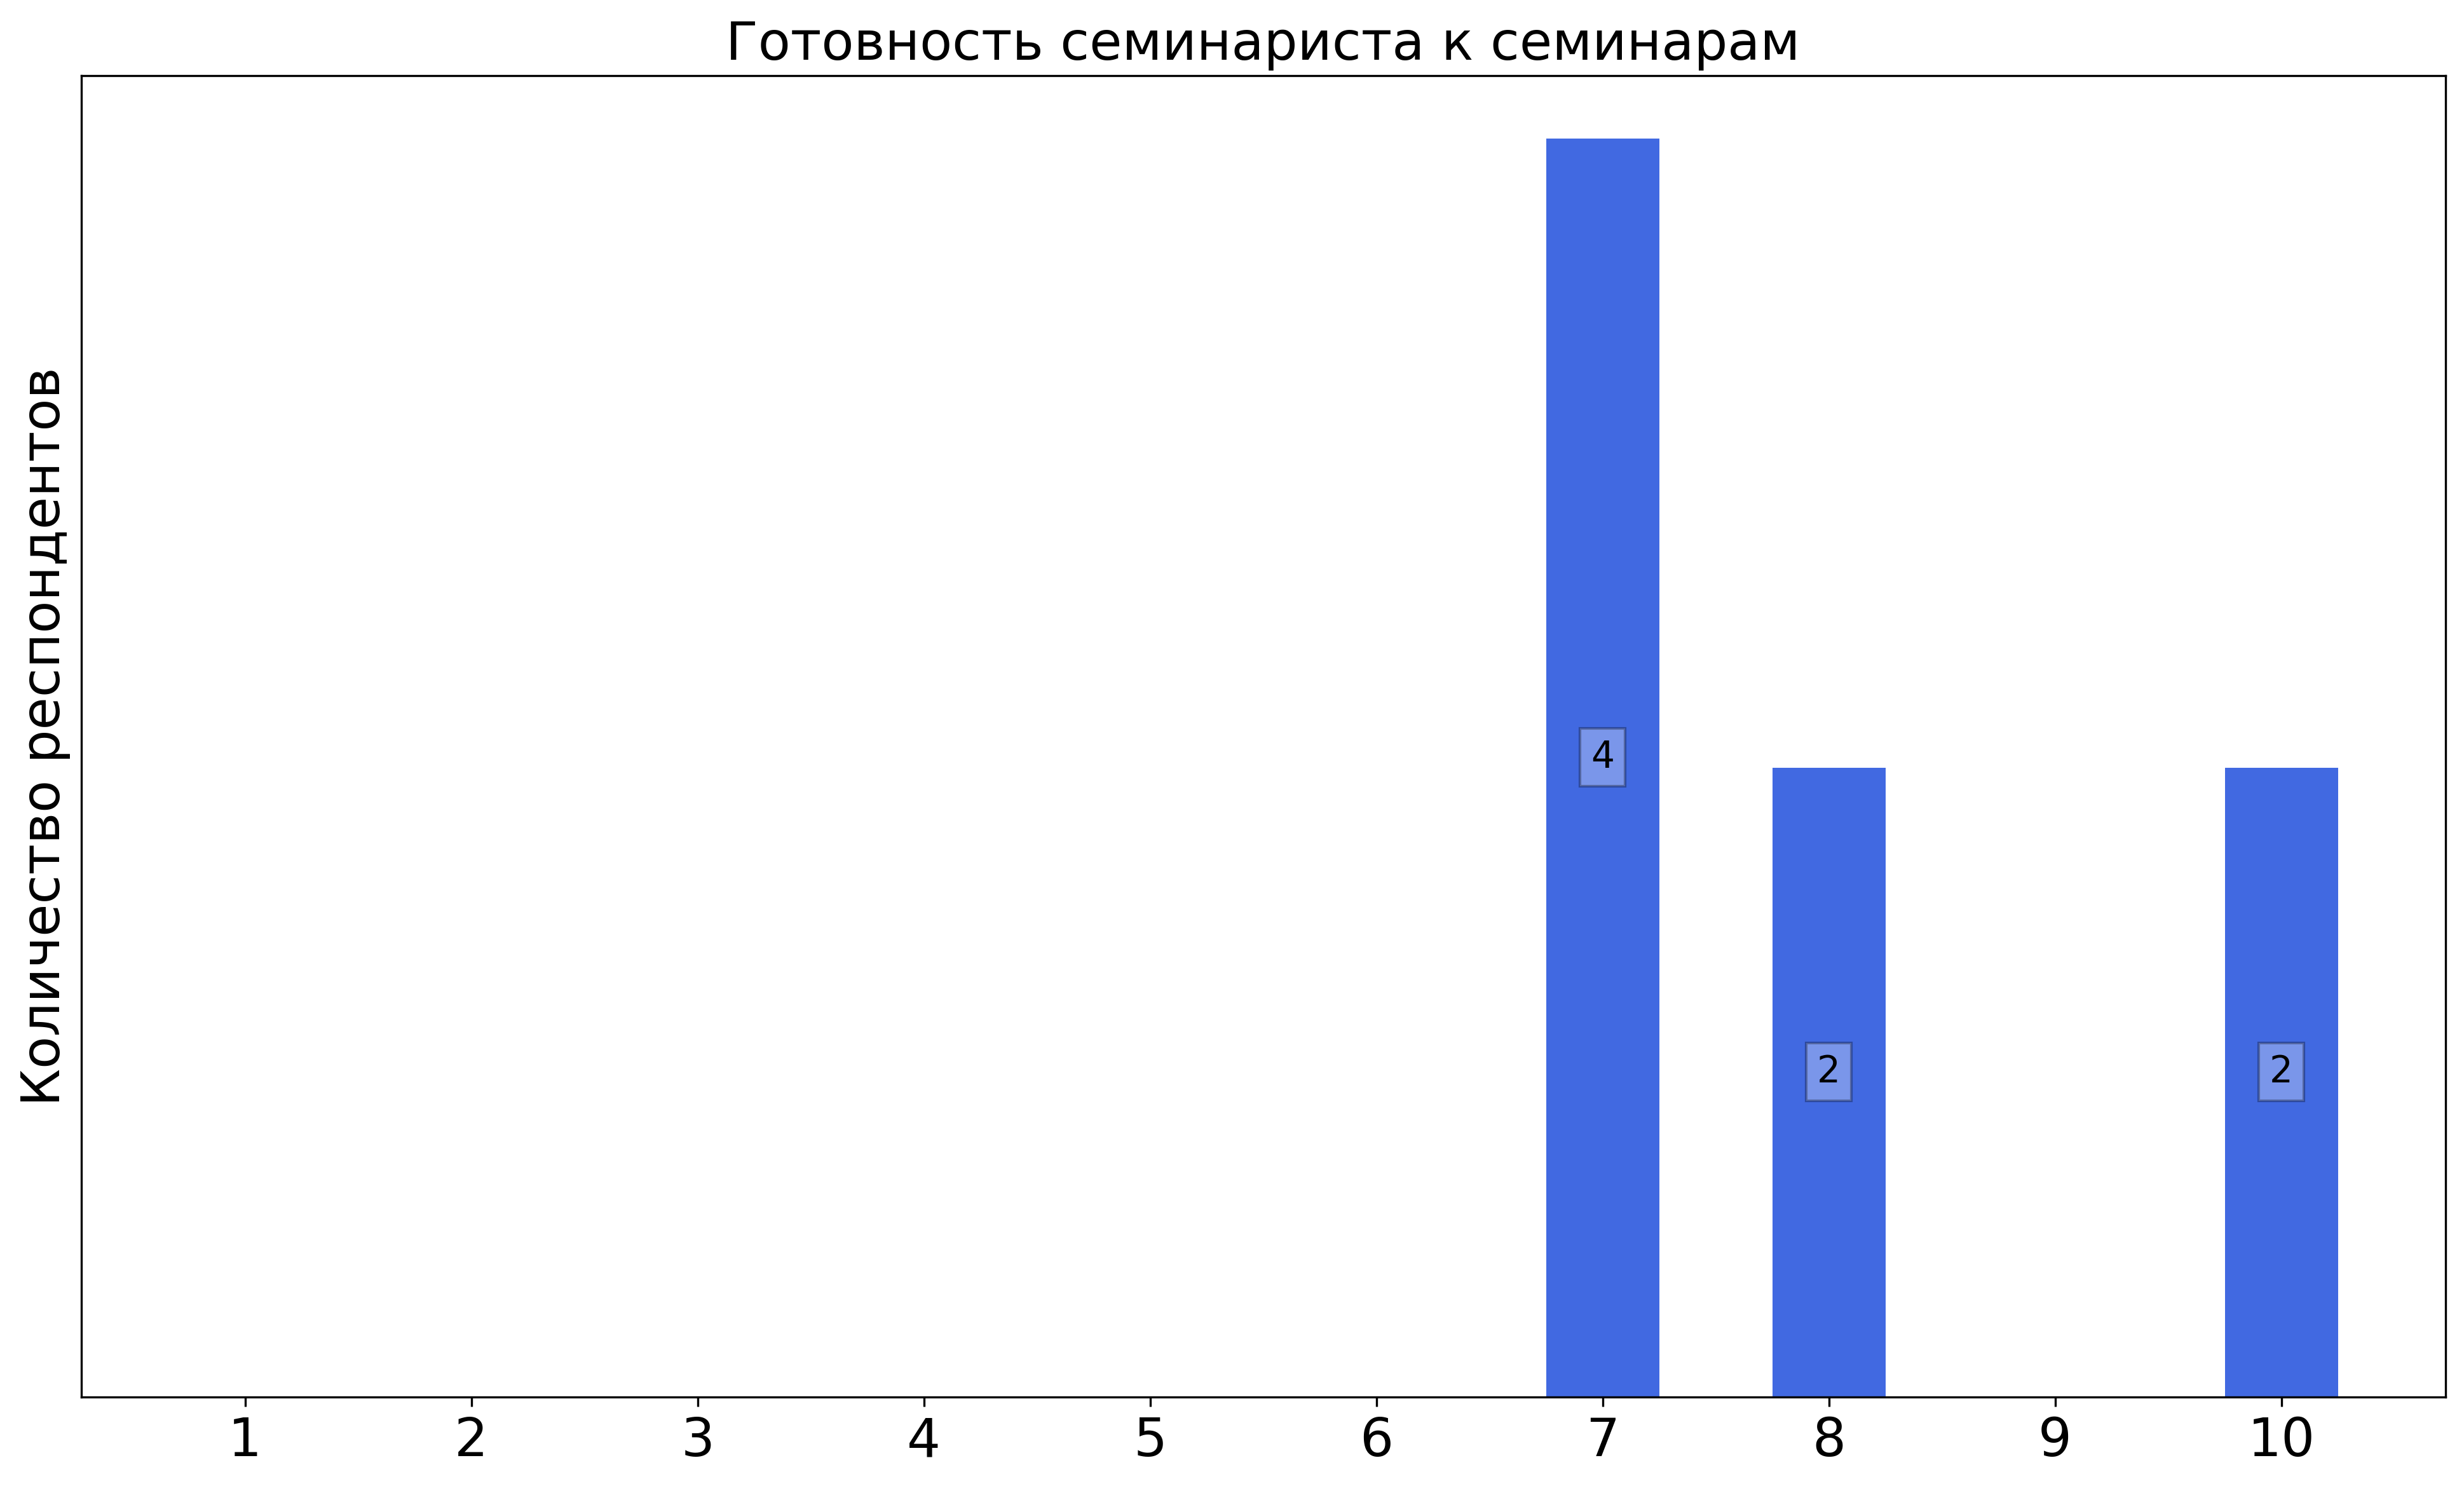
\includegraphics[width=\textwidth]{images/3 course/Общая физика - квантовая физика/seminarists-marks-Покотило И.Л.-1.png}
                \end{subfigure}
                \begin{subfigure}[b]{0.45\textwidth}
                    \centering
                    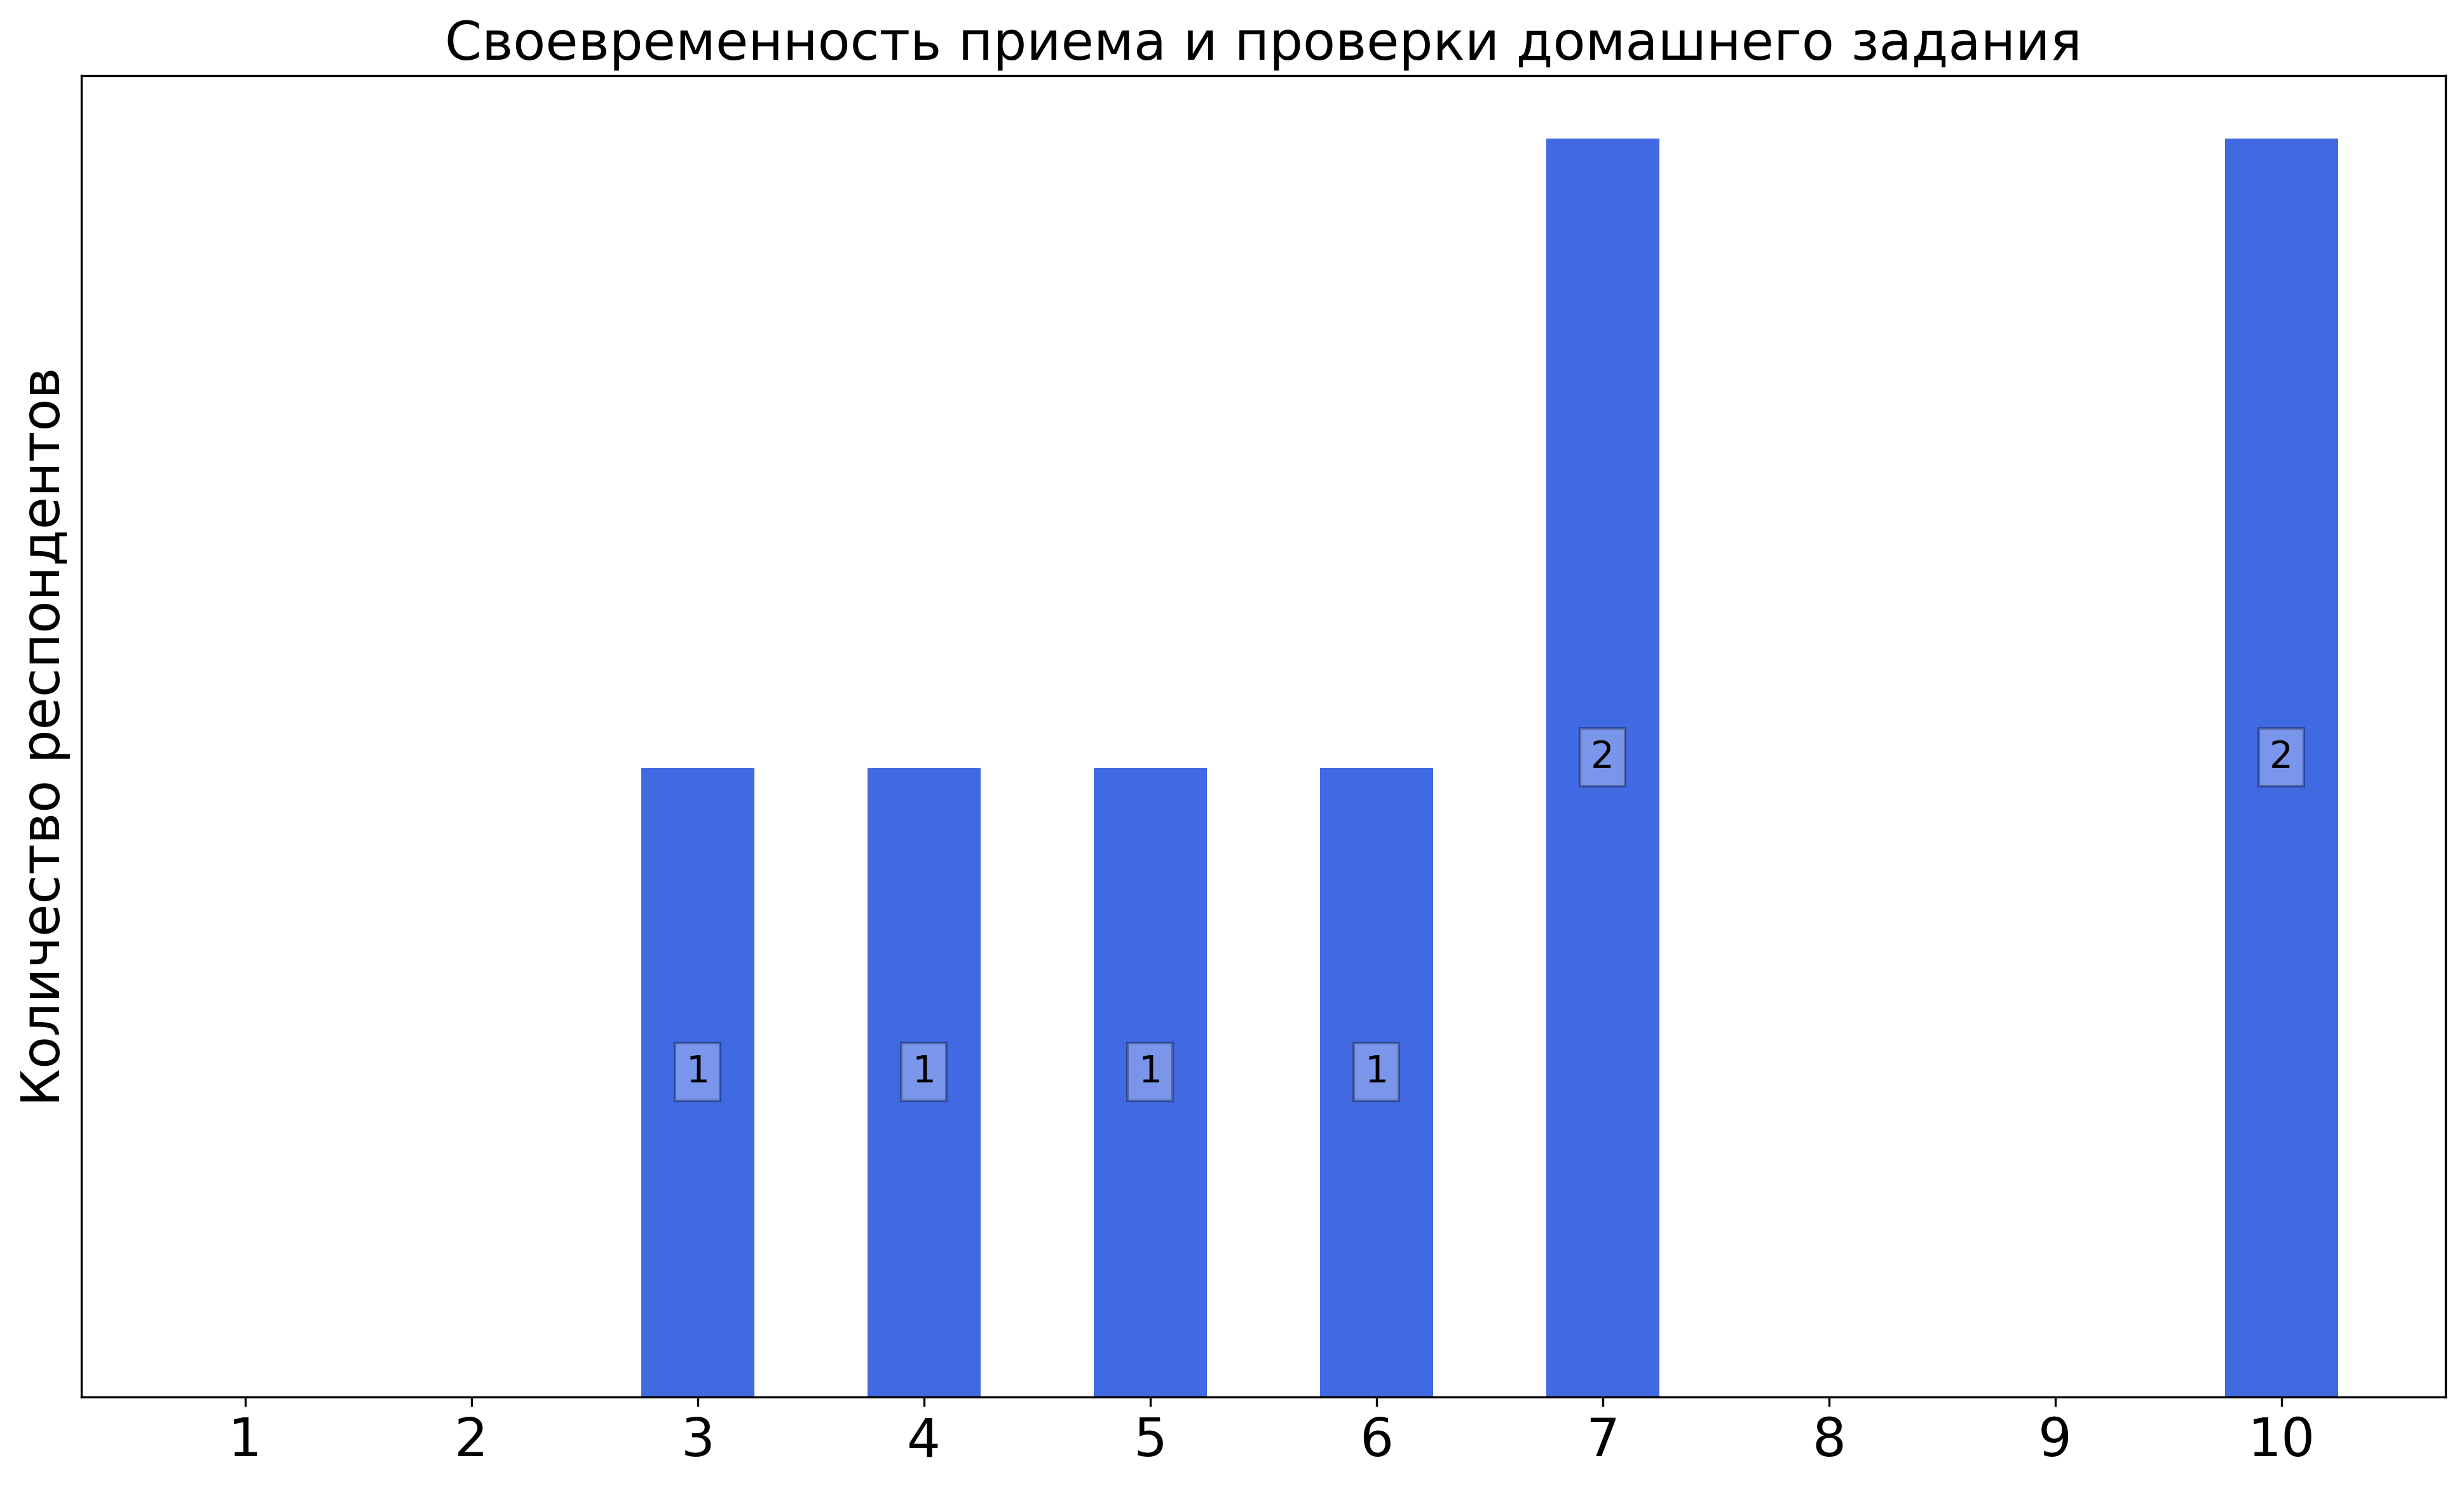
\includegraphics[width=\textwidth]{images/3 course/Общая физика - квантовая физика/seminarists-marks-Покотило И.Л.-2.png}
                \end{subfigure}
                \begin{subfigure}[b]{0.45\textwidth}
                    \centering
                    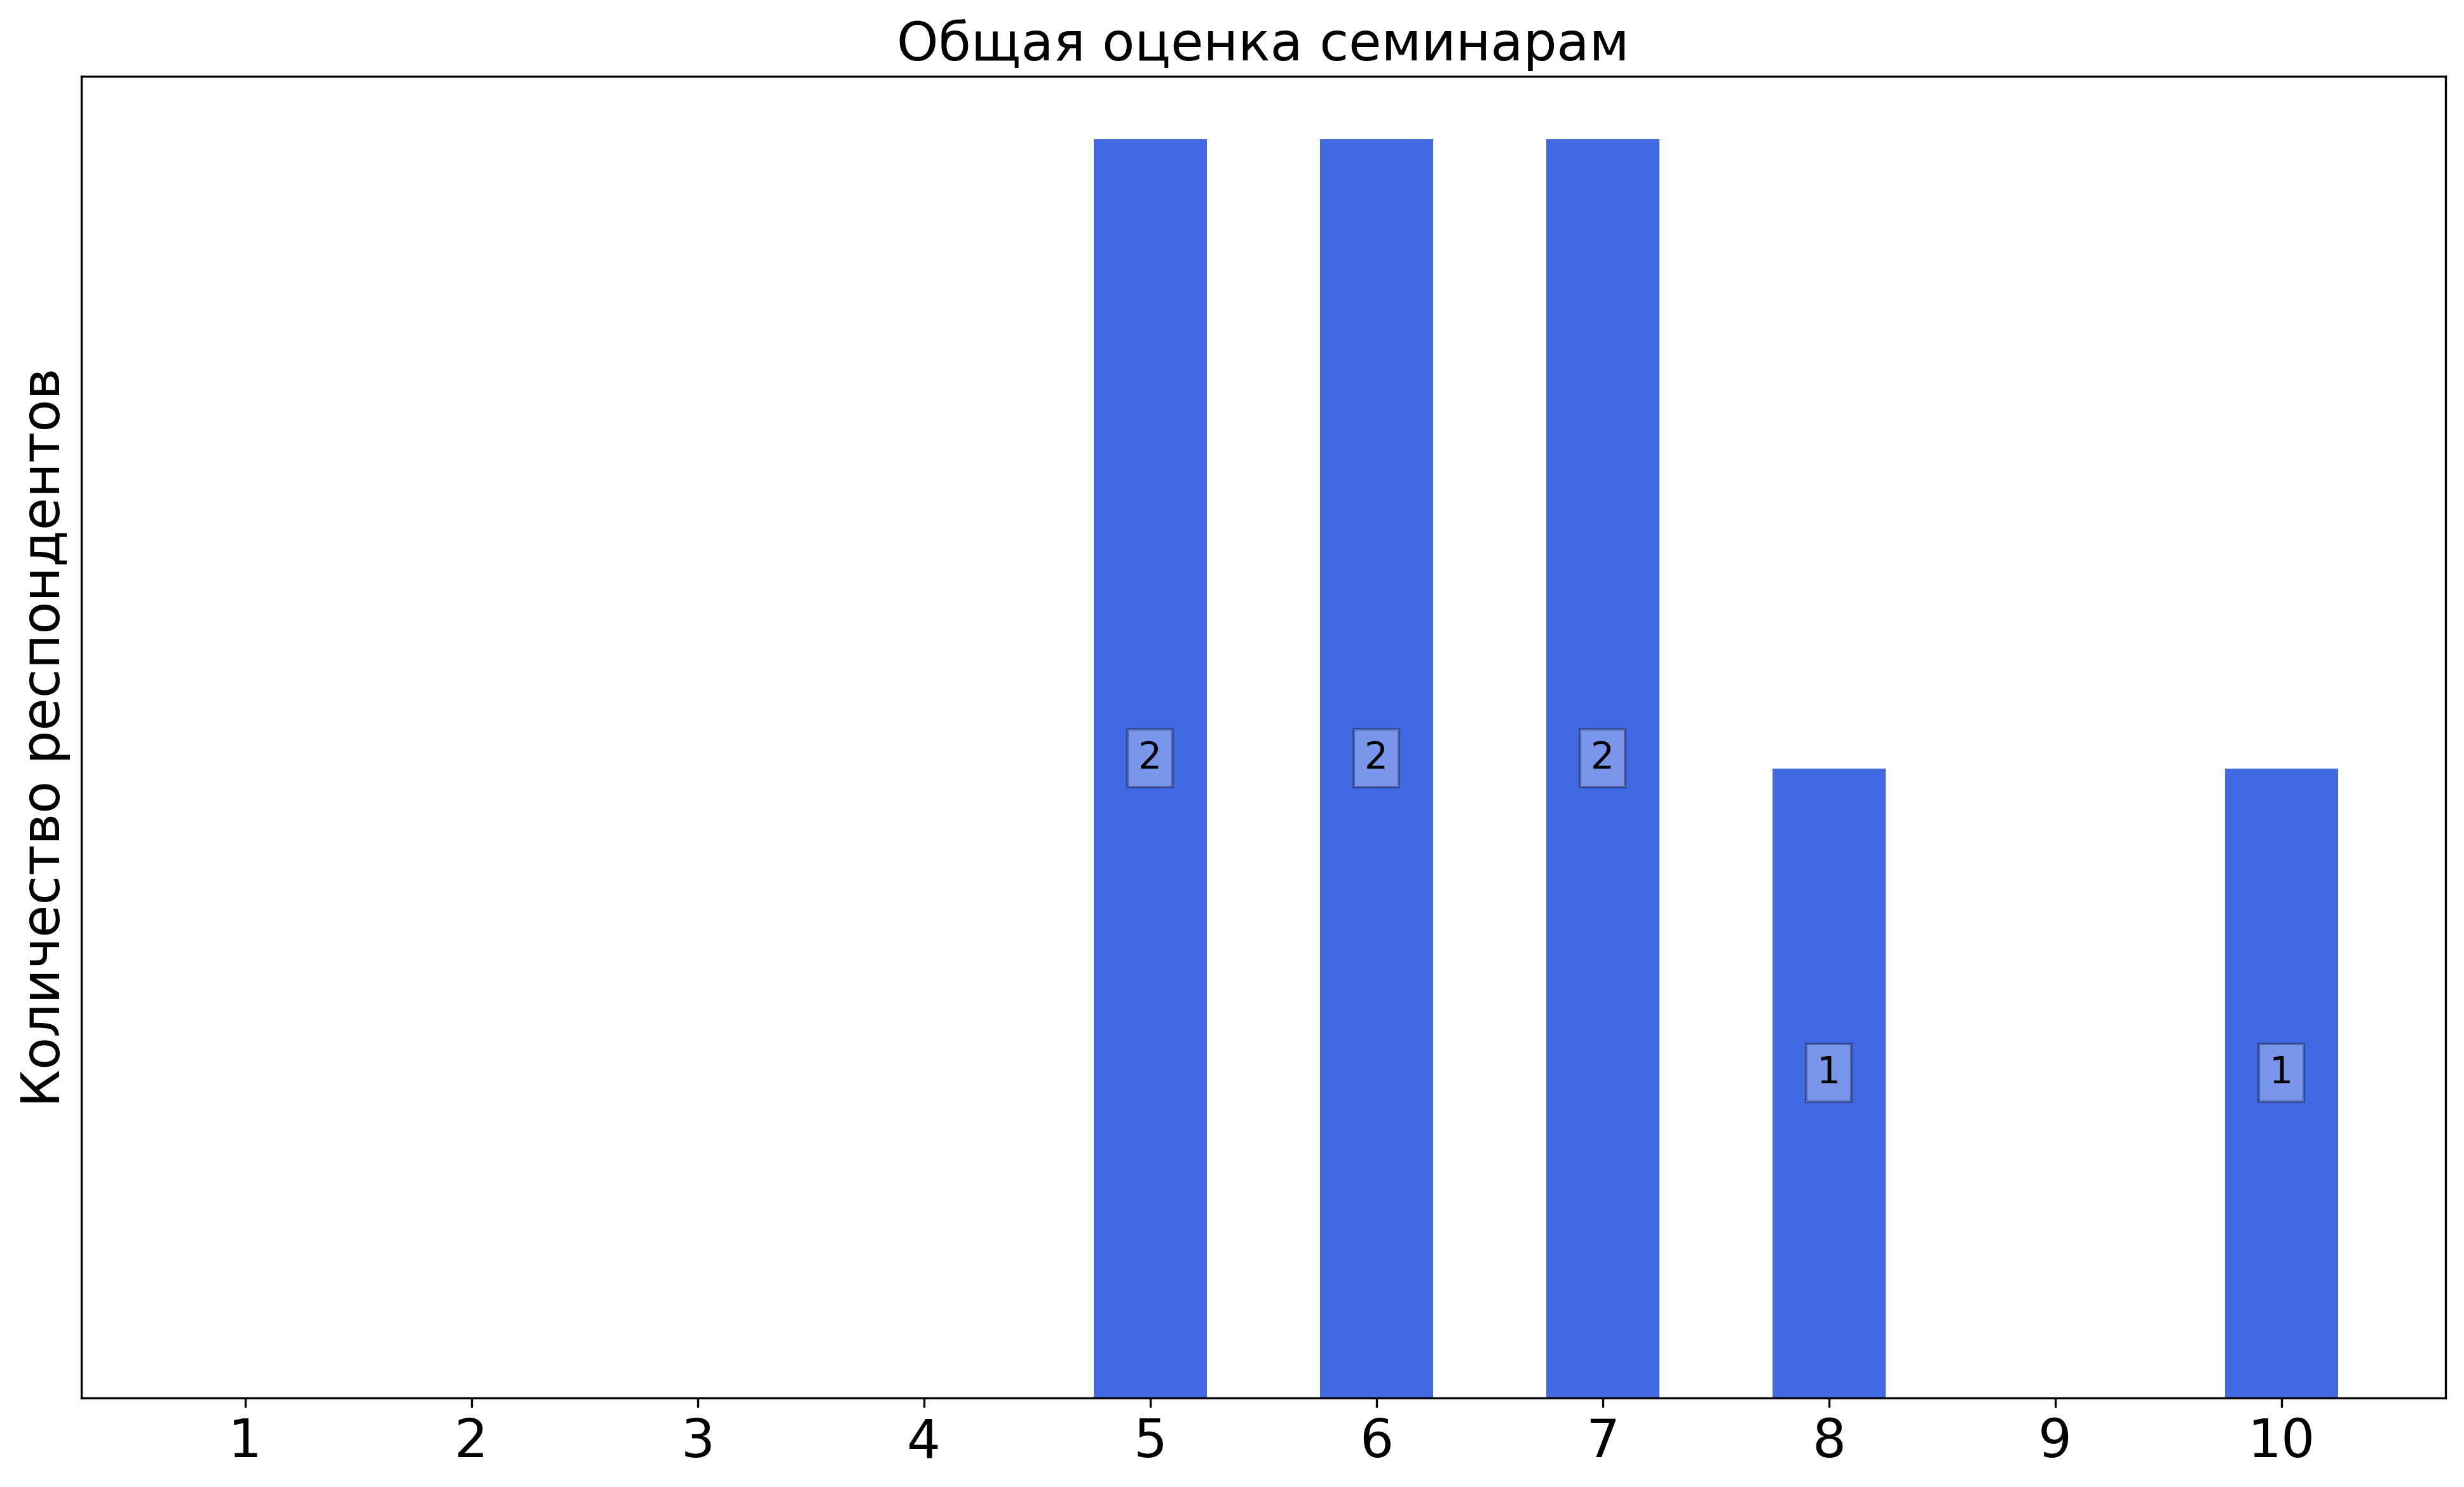
\includegraphics[width=\textwidth]{images/3 course/Общая физика - квантовая физика/seminarists-marks-Покотило И.Л.-3.png}
                \end{subfigure}	
                \caption{Оценки респондентов о качестве преподавания семинаров}
            \end{figure}

            \textbf{Комментарии студентов о семинаристе\protect\footnote{сохранены оригинальные орфография и пунктуация}}
                \begin{commentbox} 
                    Хороший преподаватель, иногда слишком много времени уделяет теории, не все успели разобрать, принимает дз опираясь на посещения семинаров. 
                \end{commentbox} 
            
                \begin{commentbox} 
                    Ирина Леонидовна разбирается в своем предмете, но семинары получается очень сумбурные из-за того, что пытается очень многое объяснить. 
                \end{commentbox} 
            
                \begin{commentbox} 
                    половину семестра не ходил на семинары, т.к. не видел смысла в этом 
                \end{commentbox} 
            
                \begin{commentbox} 
                    Покотило на своей волне, такое ощущение, что ведет семинары скорее для себя, чем для студентов. Немного душноватая. ДЗ не проверяет, контрольные сложные, оценивает своеобразно. Предмету научиться у нее тяжело, хочешь заботать кванты - иди к другому препу.
                \end{commentbox} 
            
                \begin{commentbox} 
                    Хороший семинарист, был на всех семинарах. 
                \end{commentbox} 


        \subsubsection{Отзыв студентов о семинарах. Семинарист: Стожков В.Ю.}
            \begin{figure}[H]
                \centering
                \begin{subfigure}[b]{0.45\textwidth}
                    \centering
                    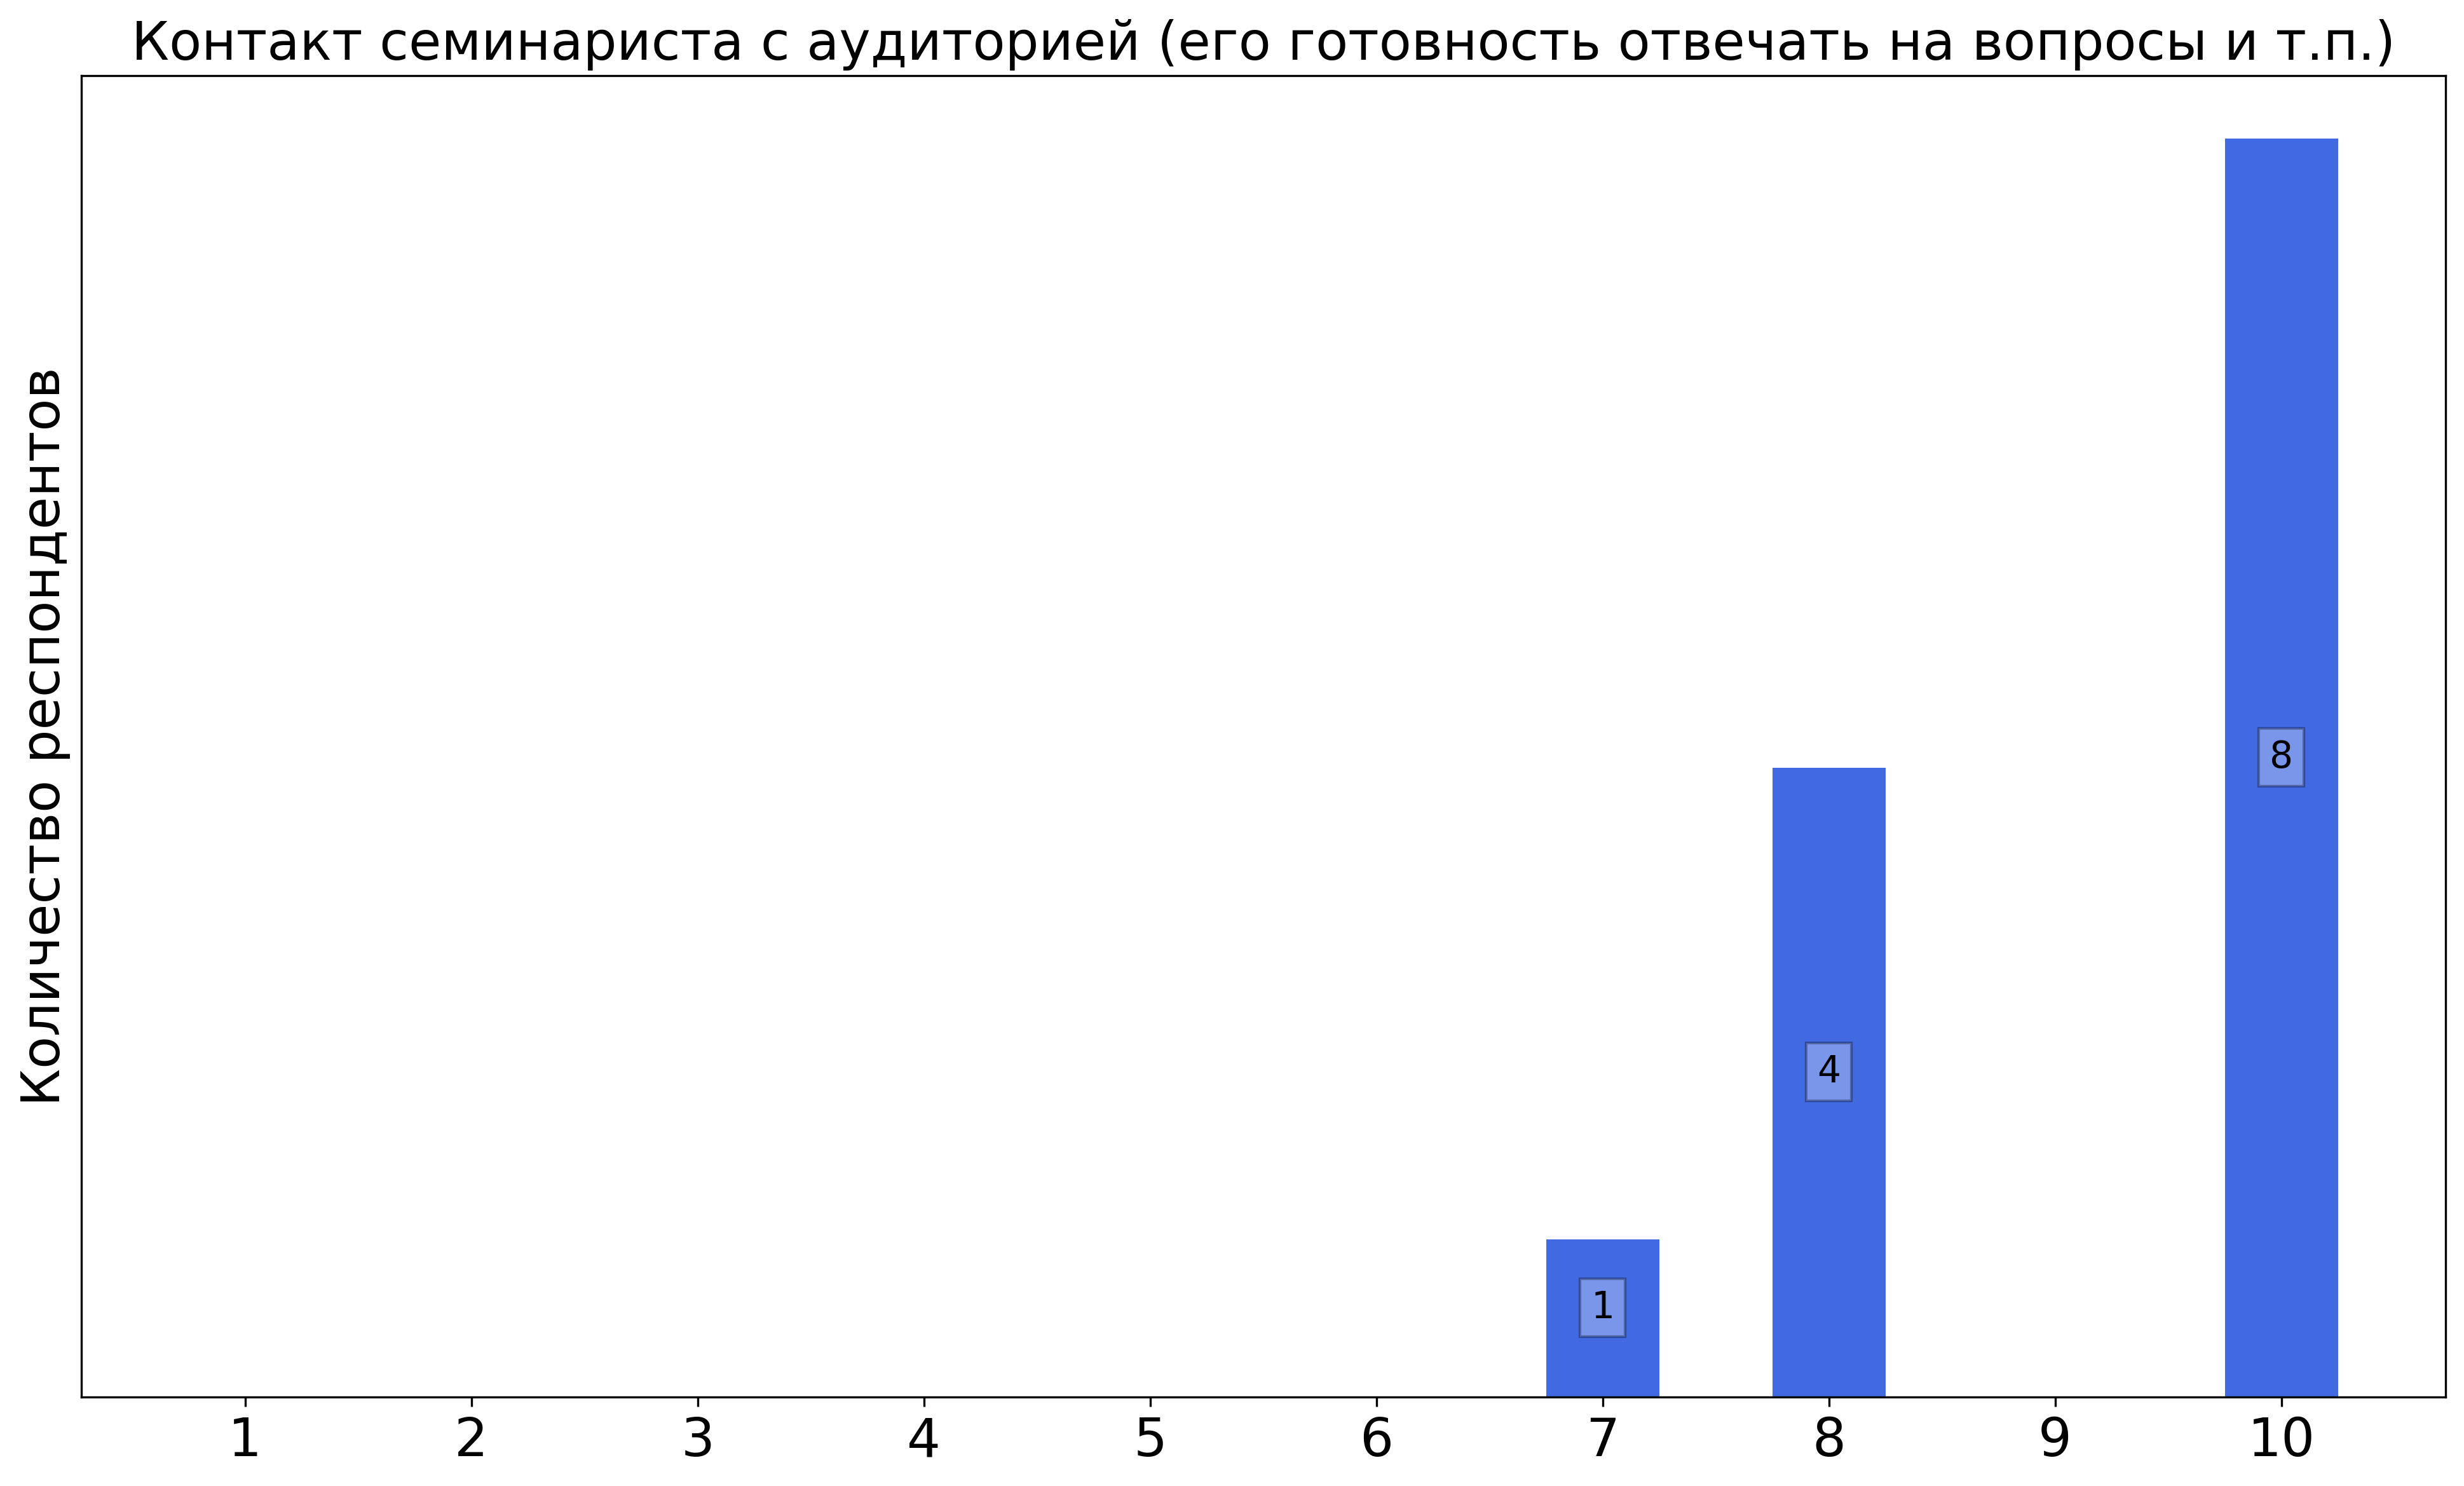
\includegraphics[width=\textwidth]{images/3 course/Общая физика - квантовая физика/seminarists-marks-Стожков В.Ю.-0.png}
                \end{subfigure}
                \begin{subfigure}[b]{0.45\textwidth}
                    \centering
                    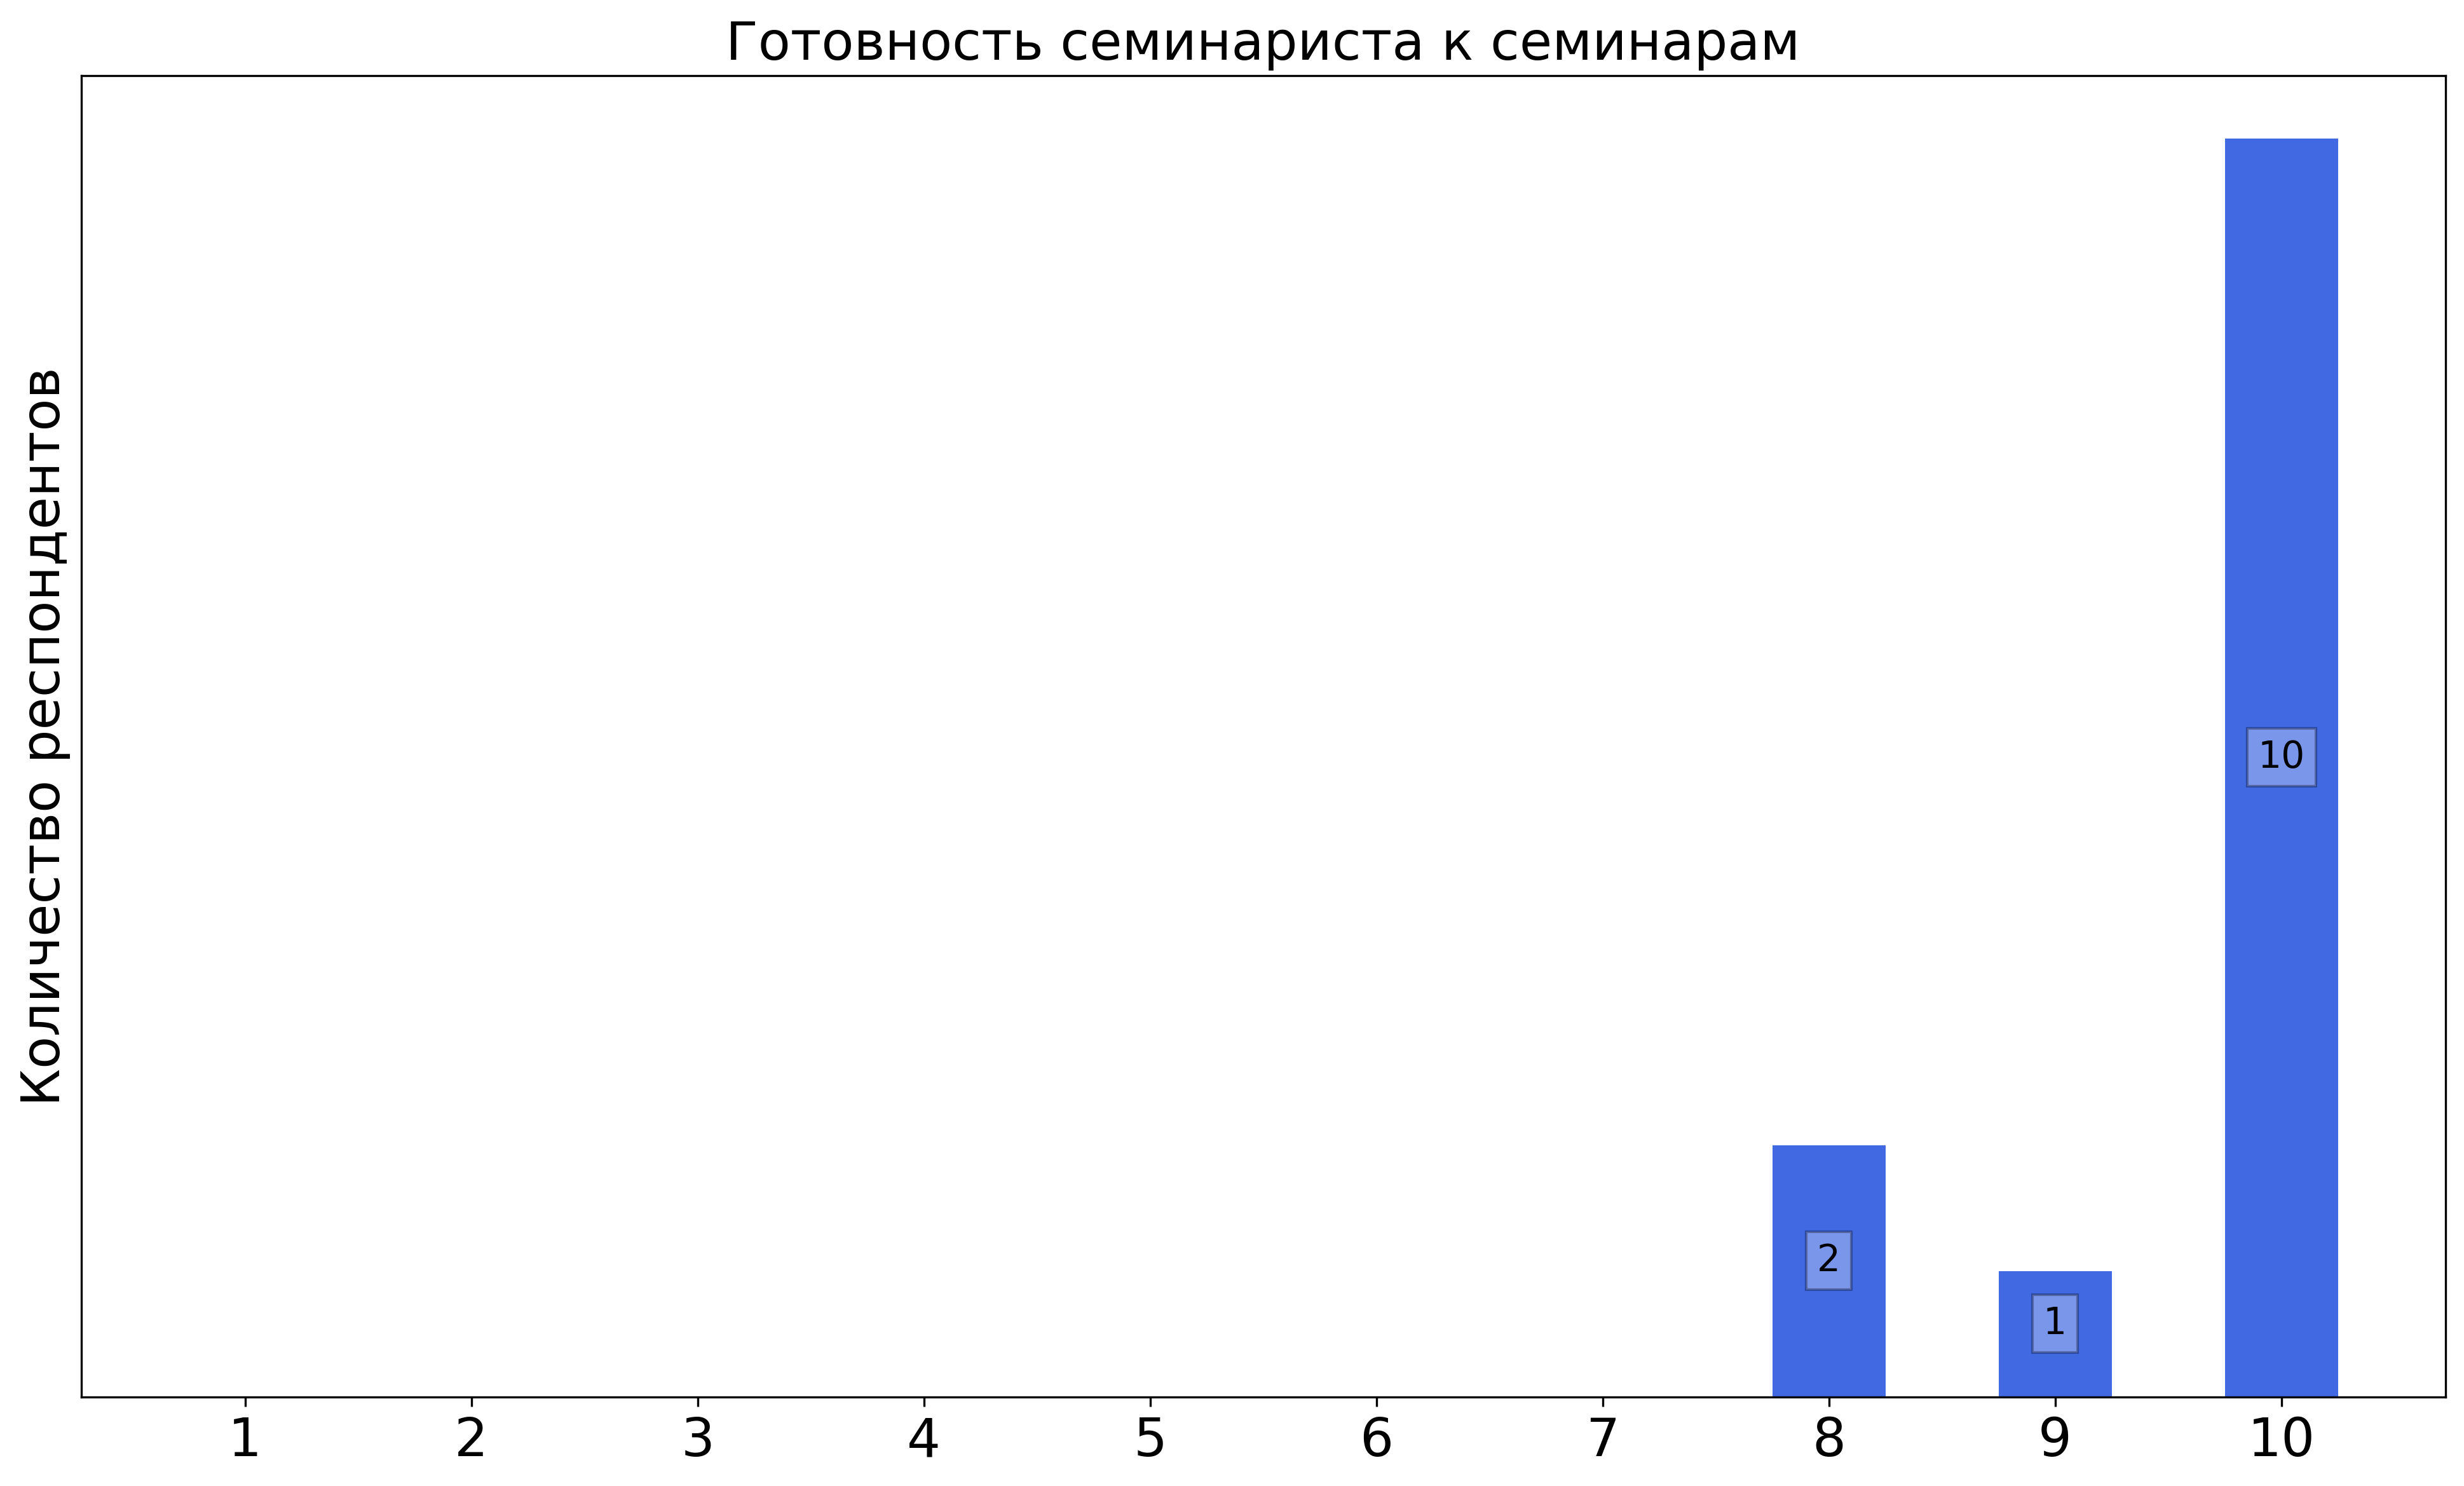
\includegraphics[width=\textwidth]{images/3 course/Общая физика - квантовая физика/seminarists-marks-Стожков В.Ю.-1.png}
                \end{subfigure}
                \begin{subfigure}[b]{0.45\textwidth}
                    \centering
                    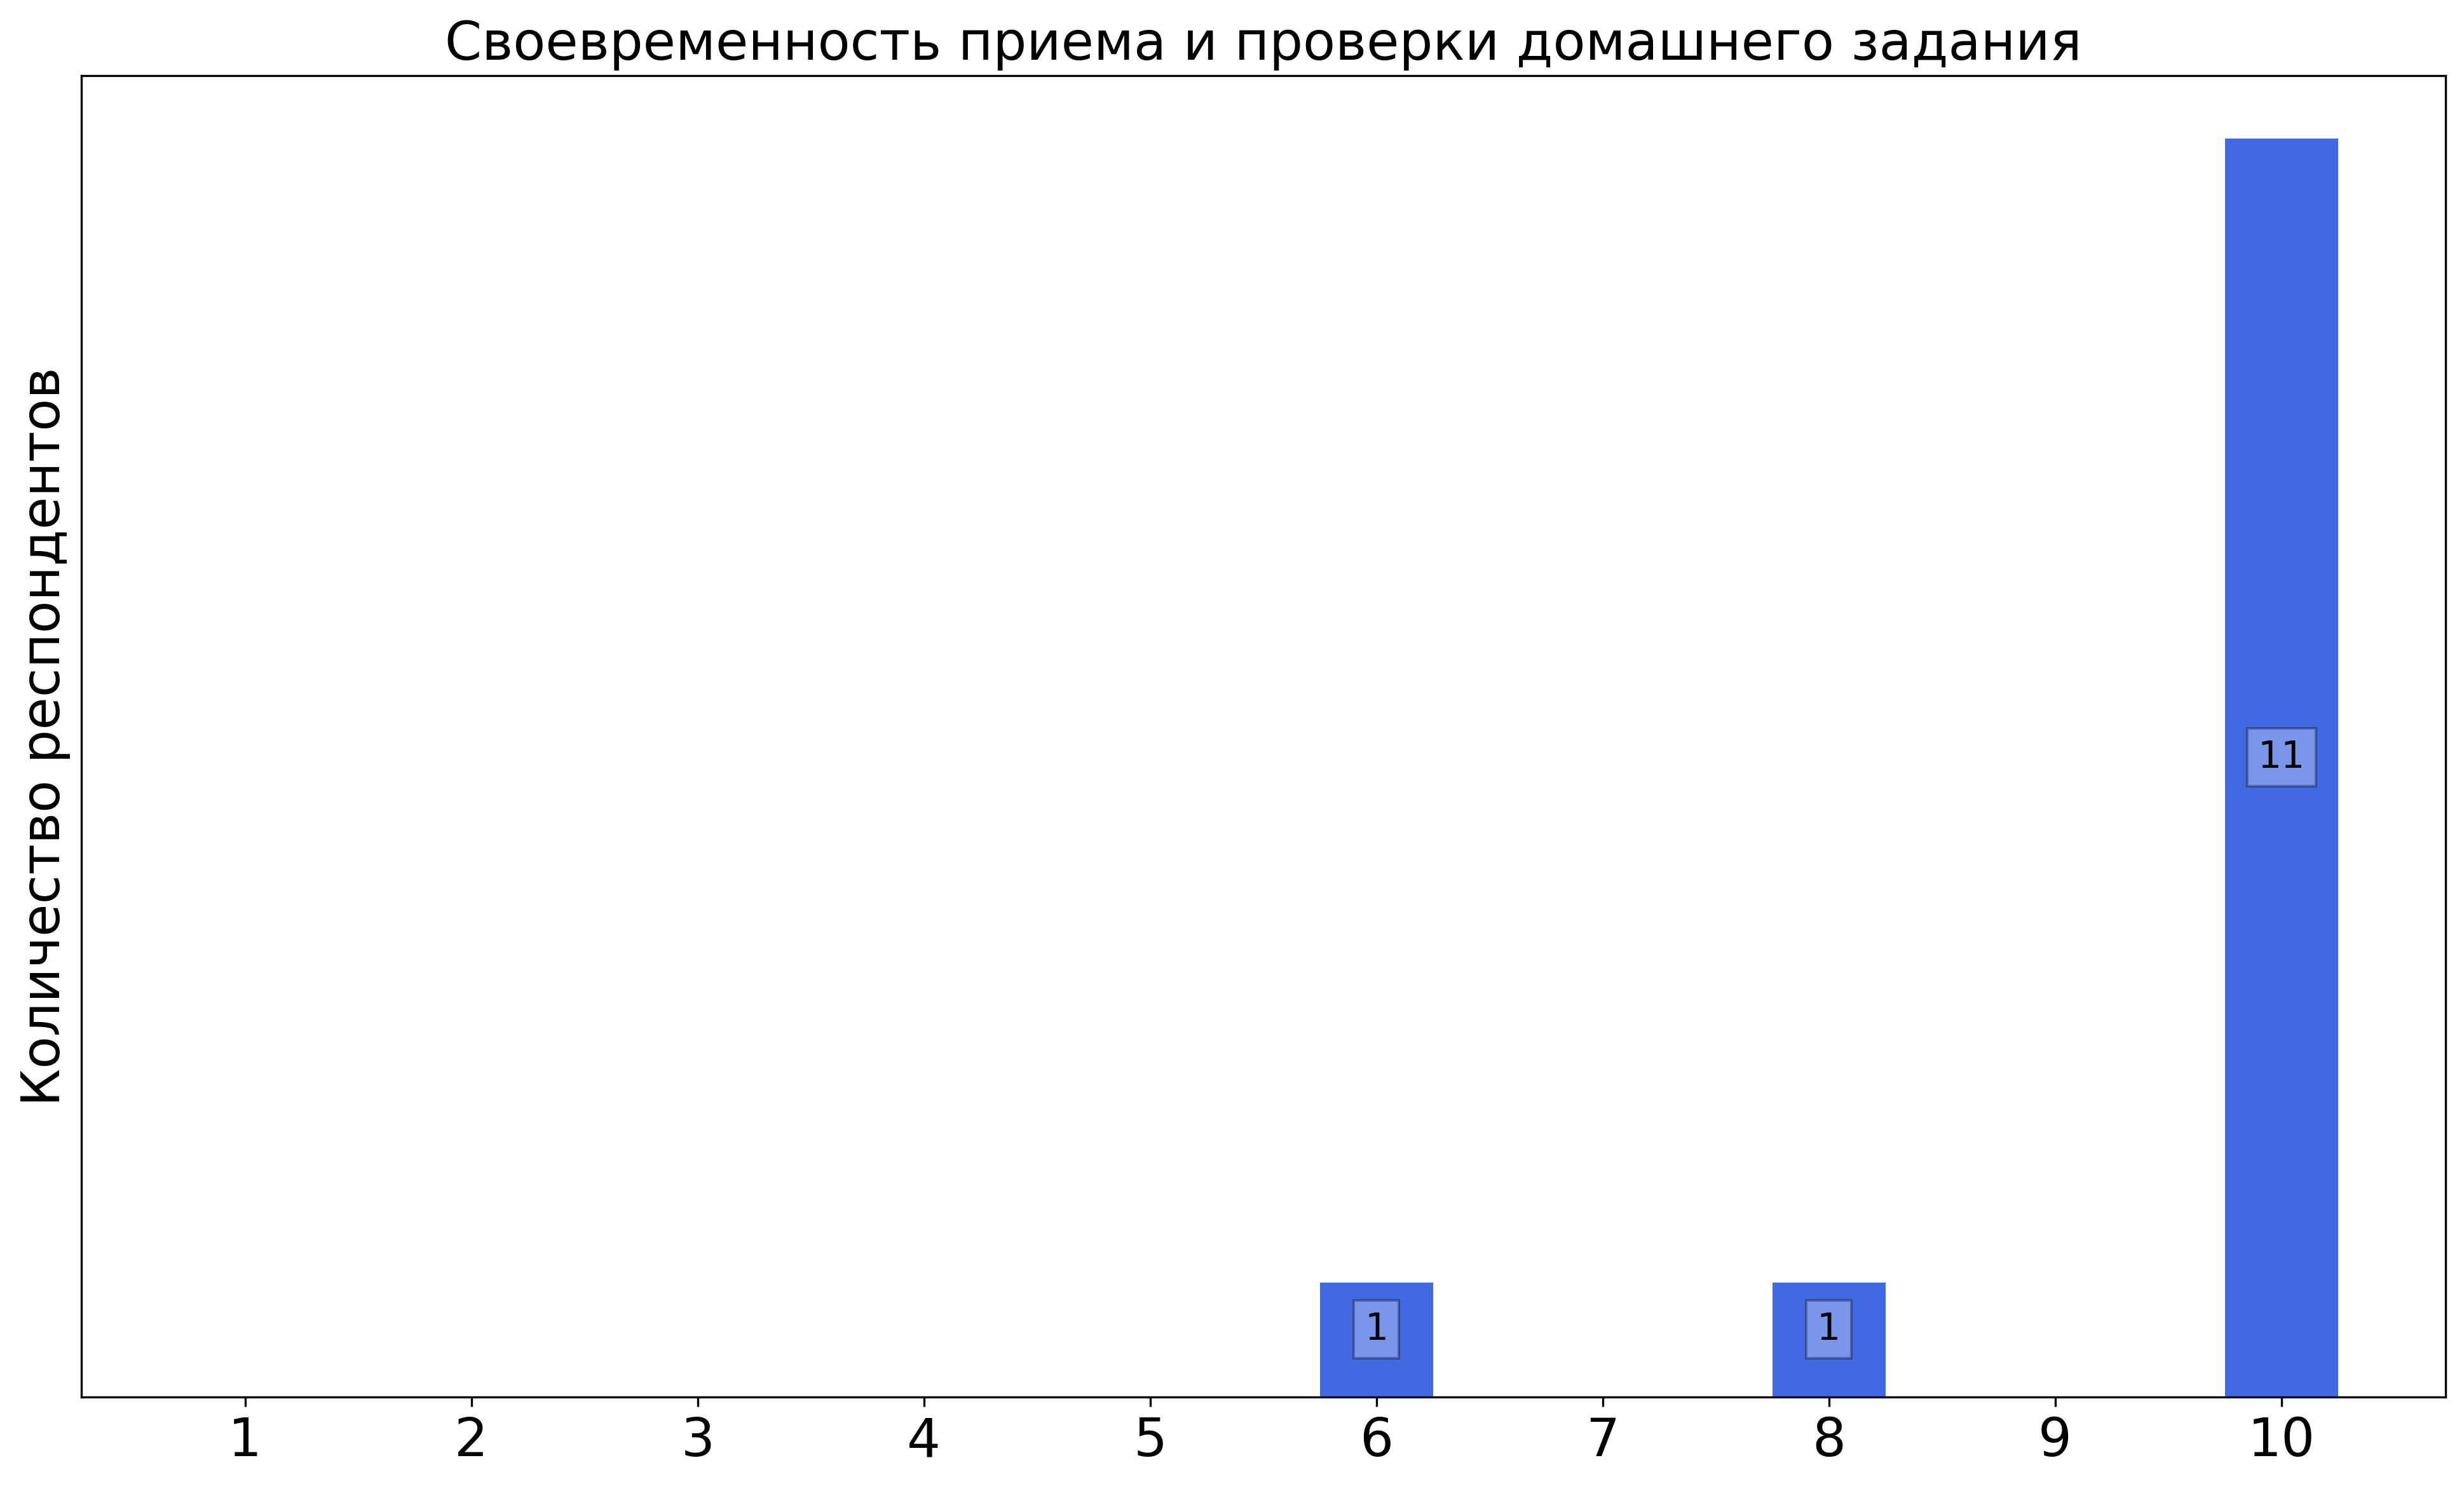
\includegraphics[width=\textwidth]{images/3 course/Общая физика - квантовая физика/seminarists-marks-Стожков В.Ю.-2.png}
                \end{subfigure}
                \begin{subfigure}[b]{0.45\textwidth}
                    \centering
                    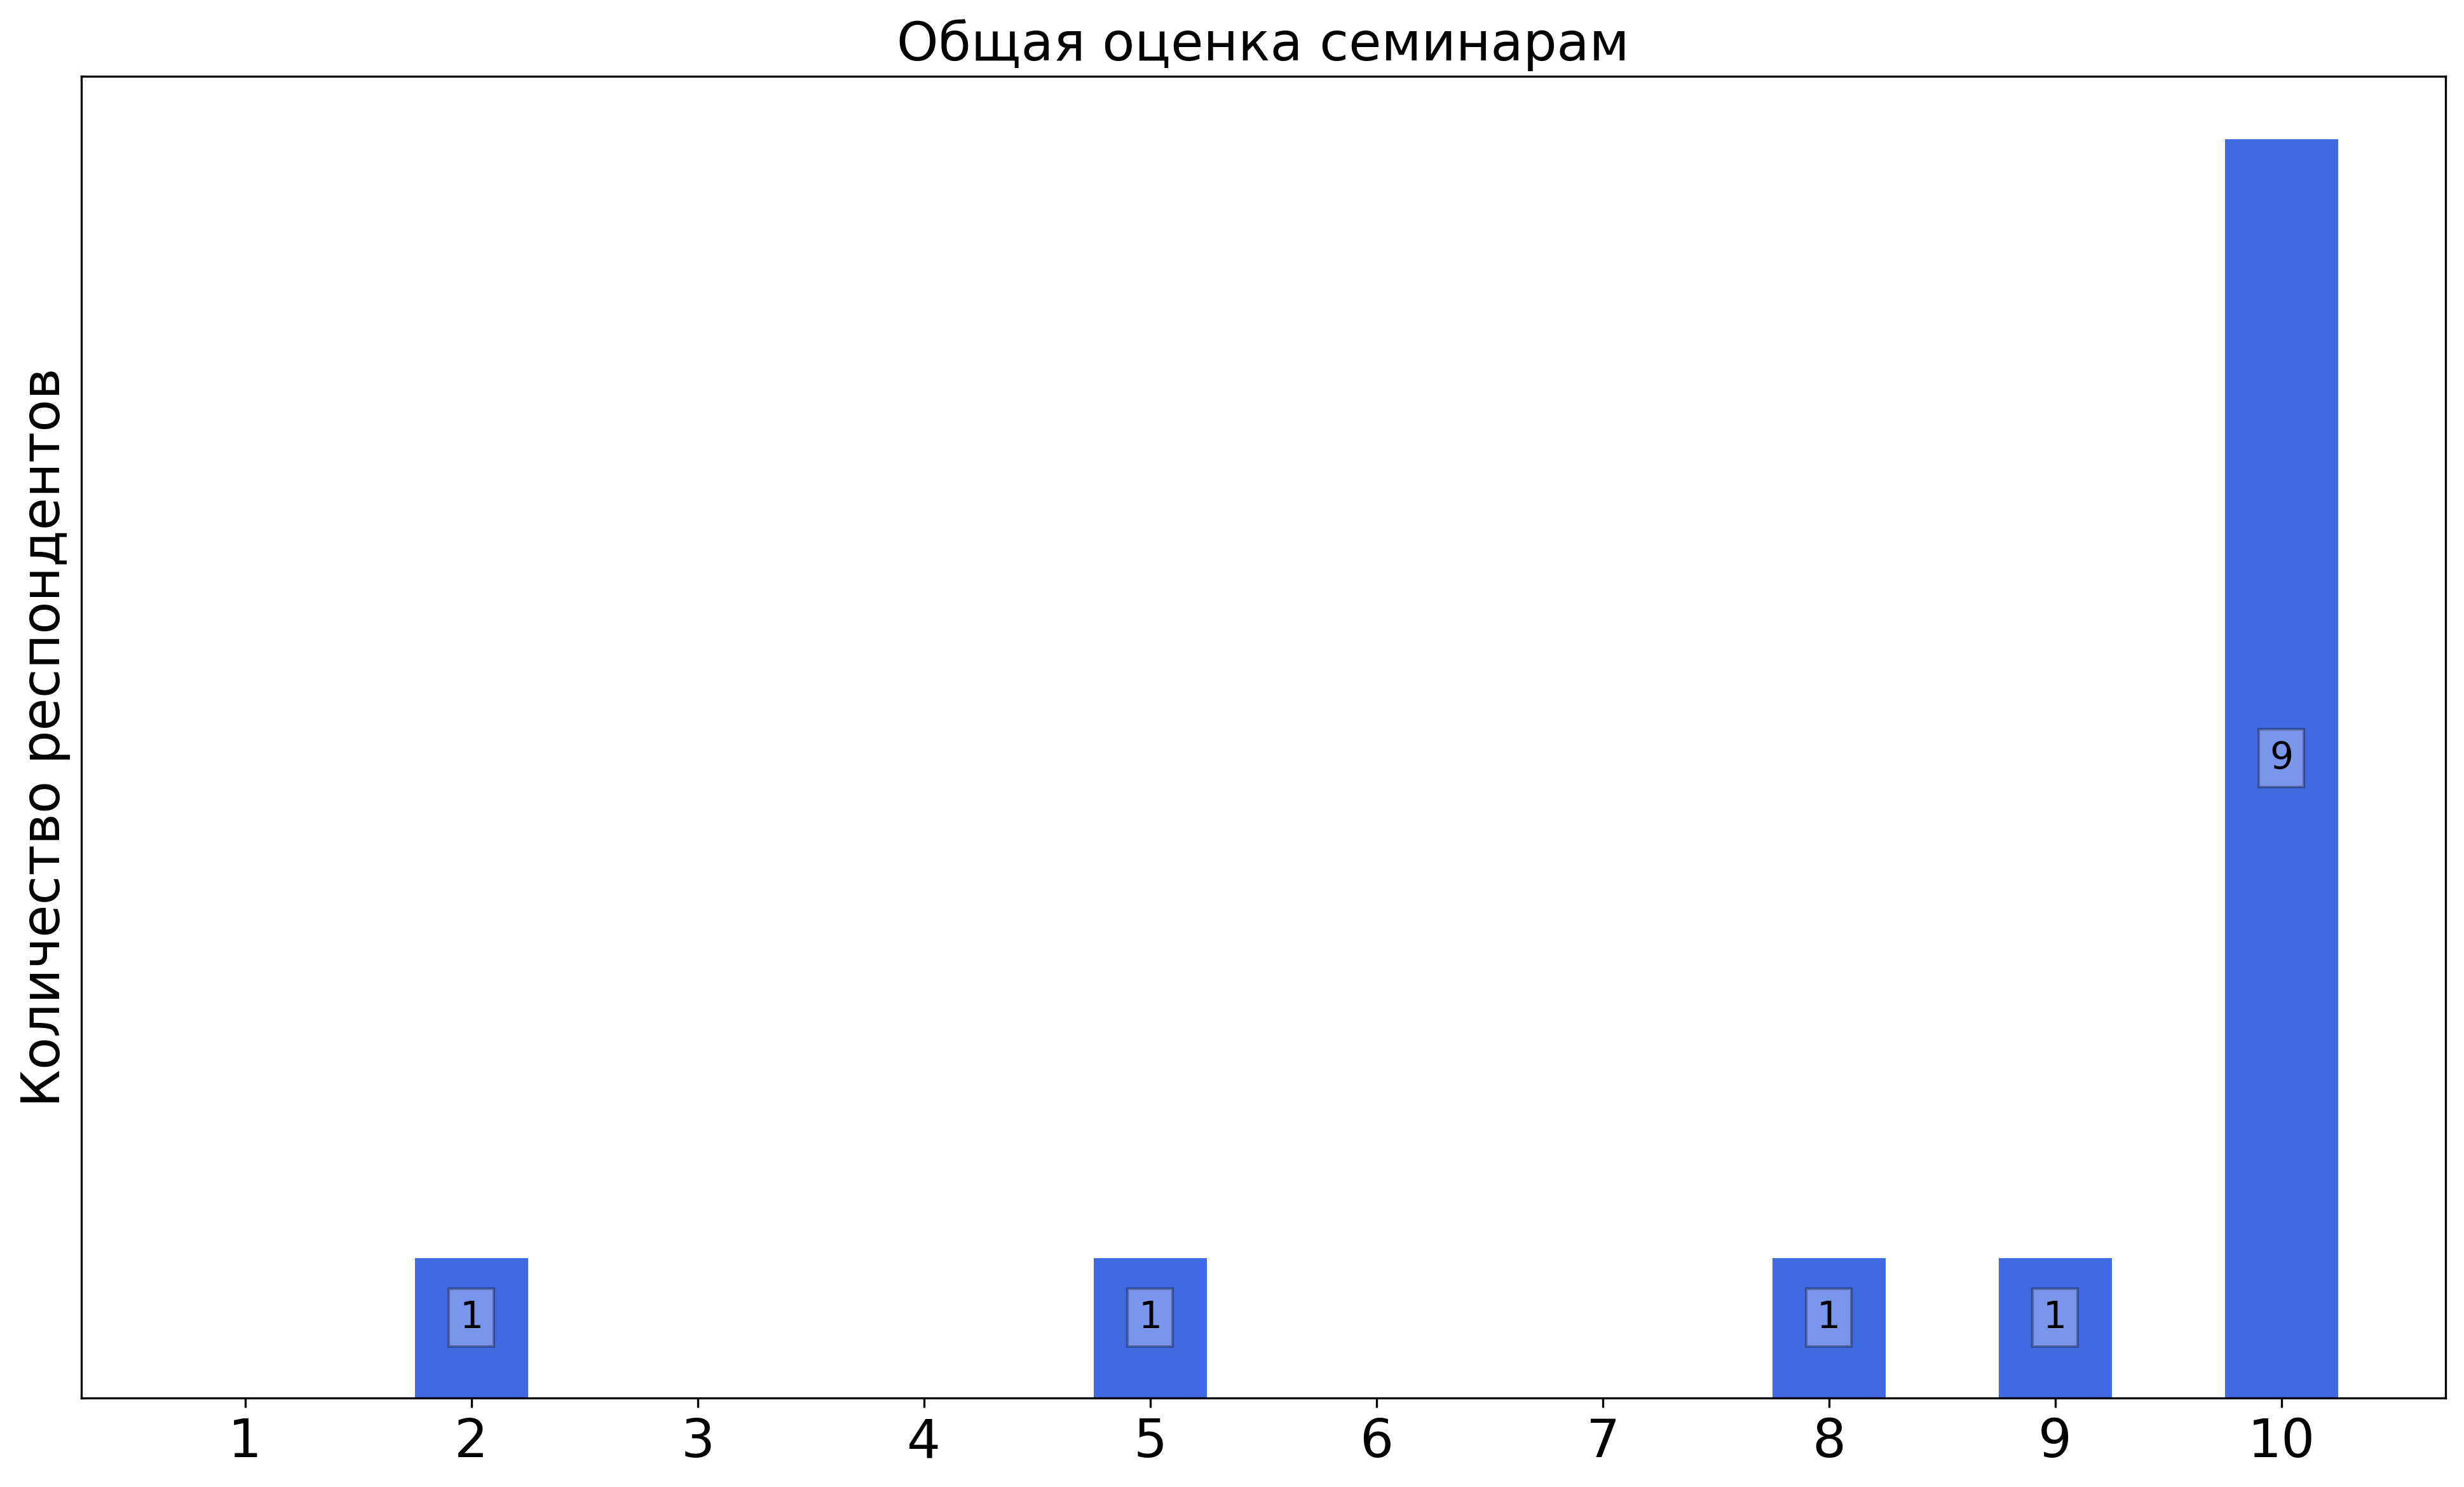
\includegraphics[width=\textwidth]{images/3 course/Общая физика - квантовая физика/seminarists-marks-Стожков В.Ю.-3.png}
                \end{subfigure}	
                \caption{Оценки респондентов о качестве преподавания семинаров}
            \end{figure}

            \textbf{Комментарии студентов о семинаристе\protect\footnote{сохранены оригинальные орфография и пунктуация}}
                \begin{commentbox} 
                    Говорит для меня весьма непонятно, но как семинарист очень халявный и как человек приятный. На сдачах дз и коллоквиуме приходилось ботать, поэтому в целом предмет был выучен 
                \end{commentbox} 

                \begin{commentbox} 
                    Стожков все также великолепен 
                \end{commentbox} 

                \begin{commentbox} 
                    Я была на паре семинарах Стожкова и поняла, что мне формат его семинаров абсолютно не подходит, он рассказывает очень быстро, почти без теор справки, поэтому мало что остаётся понятным(поэтому я перевелась к Жабину С.Н.) 
                \end{commentbox} 

                \begin{commentbox} 
                    Не проводил контрольные на семинарах, из-за чего добавилось 2 семинара на разбор тем. Рассказывает довольно быстро, но скорее дело в специфике дисциплины (слишком большой объем материала). Были сдачи дз отдельно от пар (максимум 2 человека одновременно). 
                \end{commentbox} 

    
        \subsubsection{Отзыв студентов о лабораторных работах. Преподаватель: Аникин Ю.А.}
            \begin{figure}[H]
                \centering
                \begin{subfigure}[b]{0.45\textwidth}
                    \centering
                    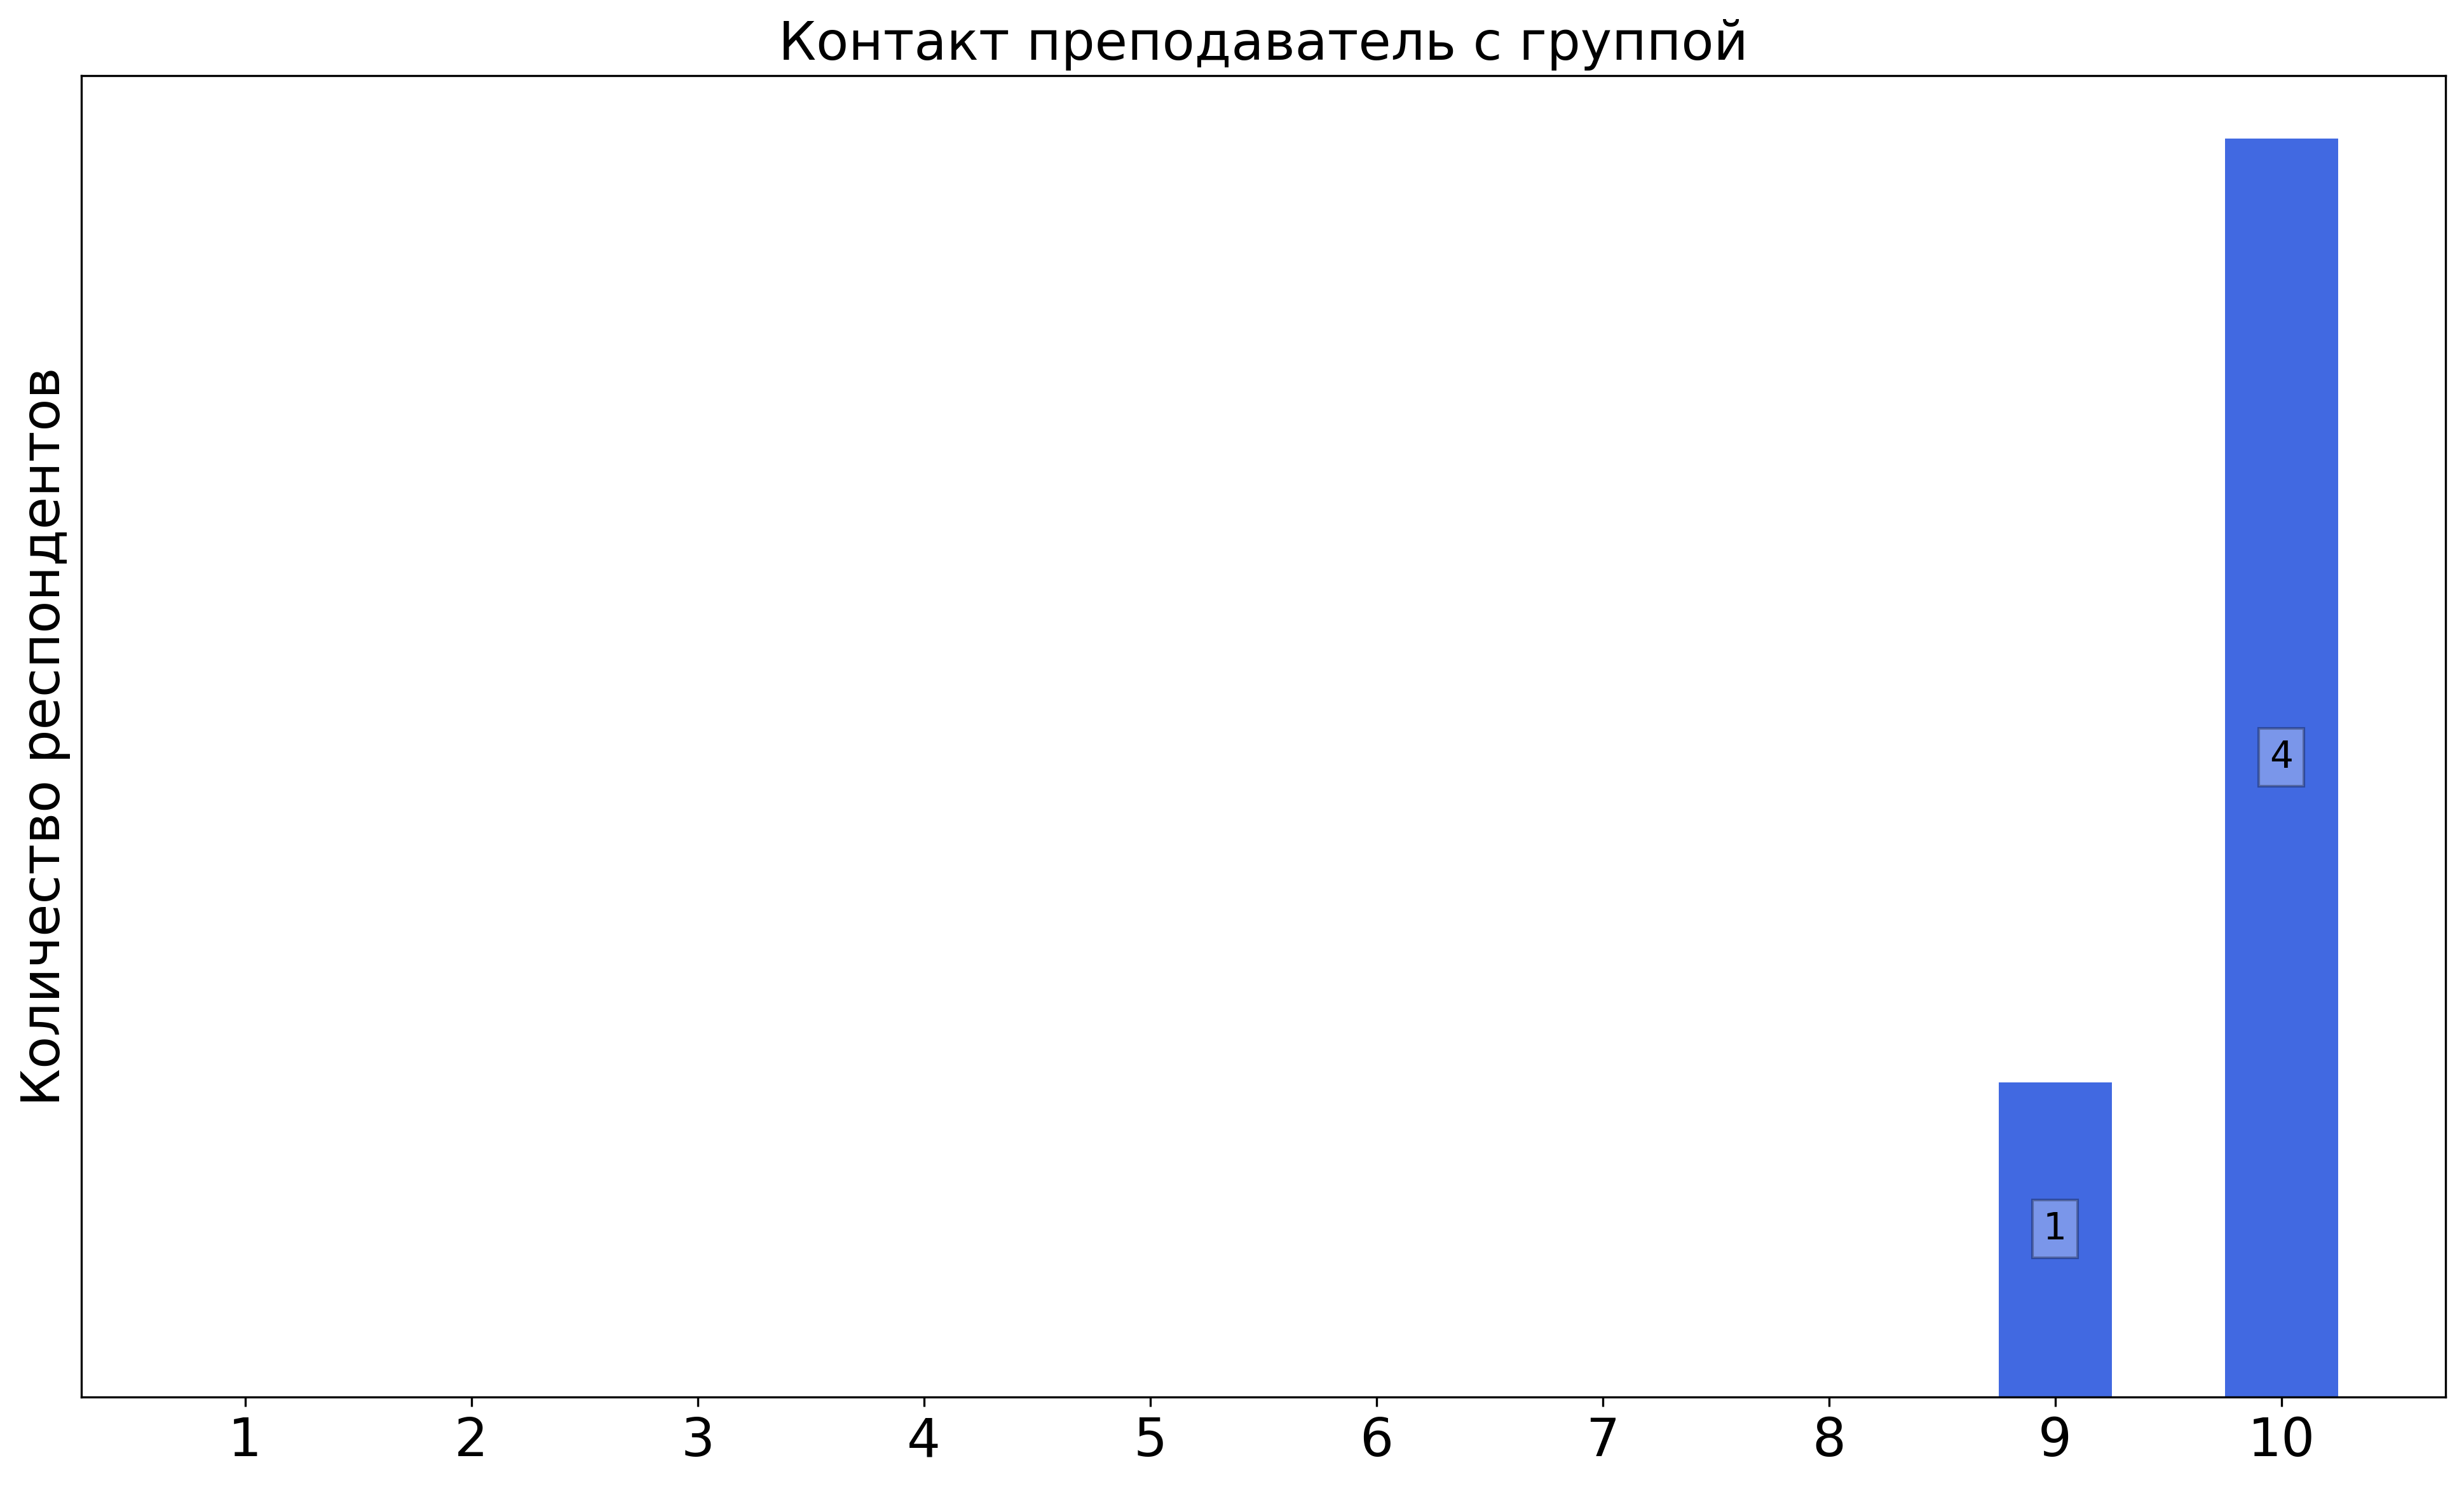
\includegraphics[width=\textwidth]{images/3 course/Общая физика - квантовая физика/labniks-marks-Аникин Ю.А.-0.png}
                \end{subfigure}
                \begin{subfigure}[b]{0.45\textwidth}
                    \centering
                    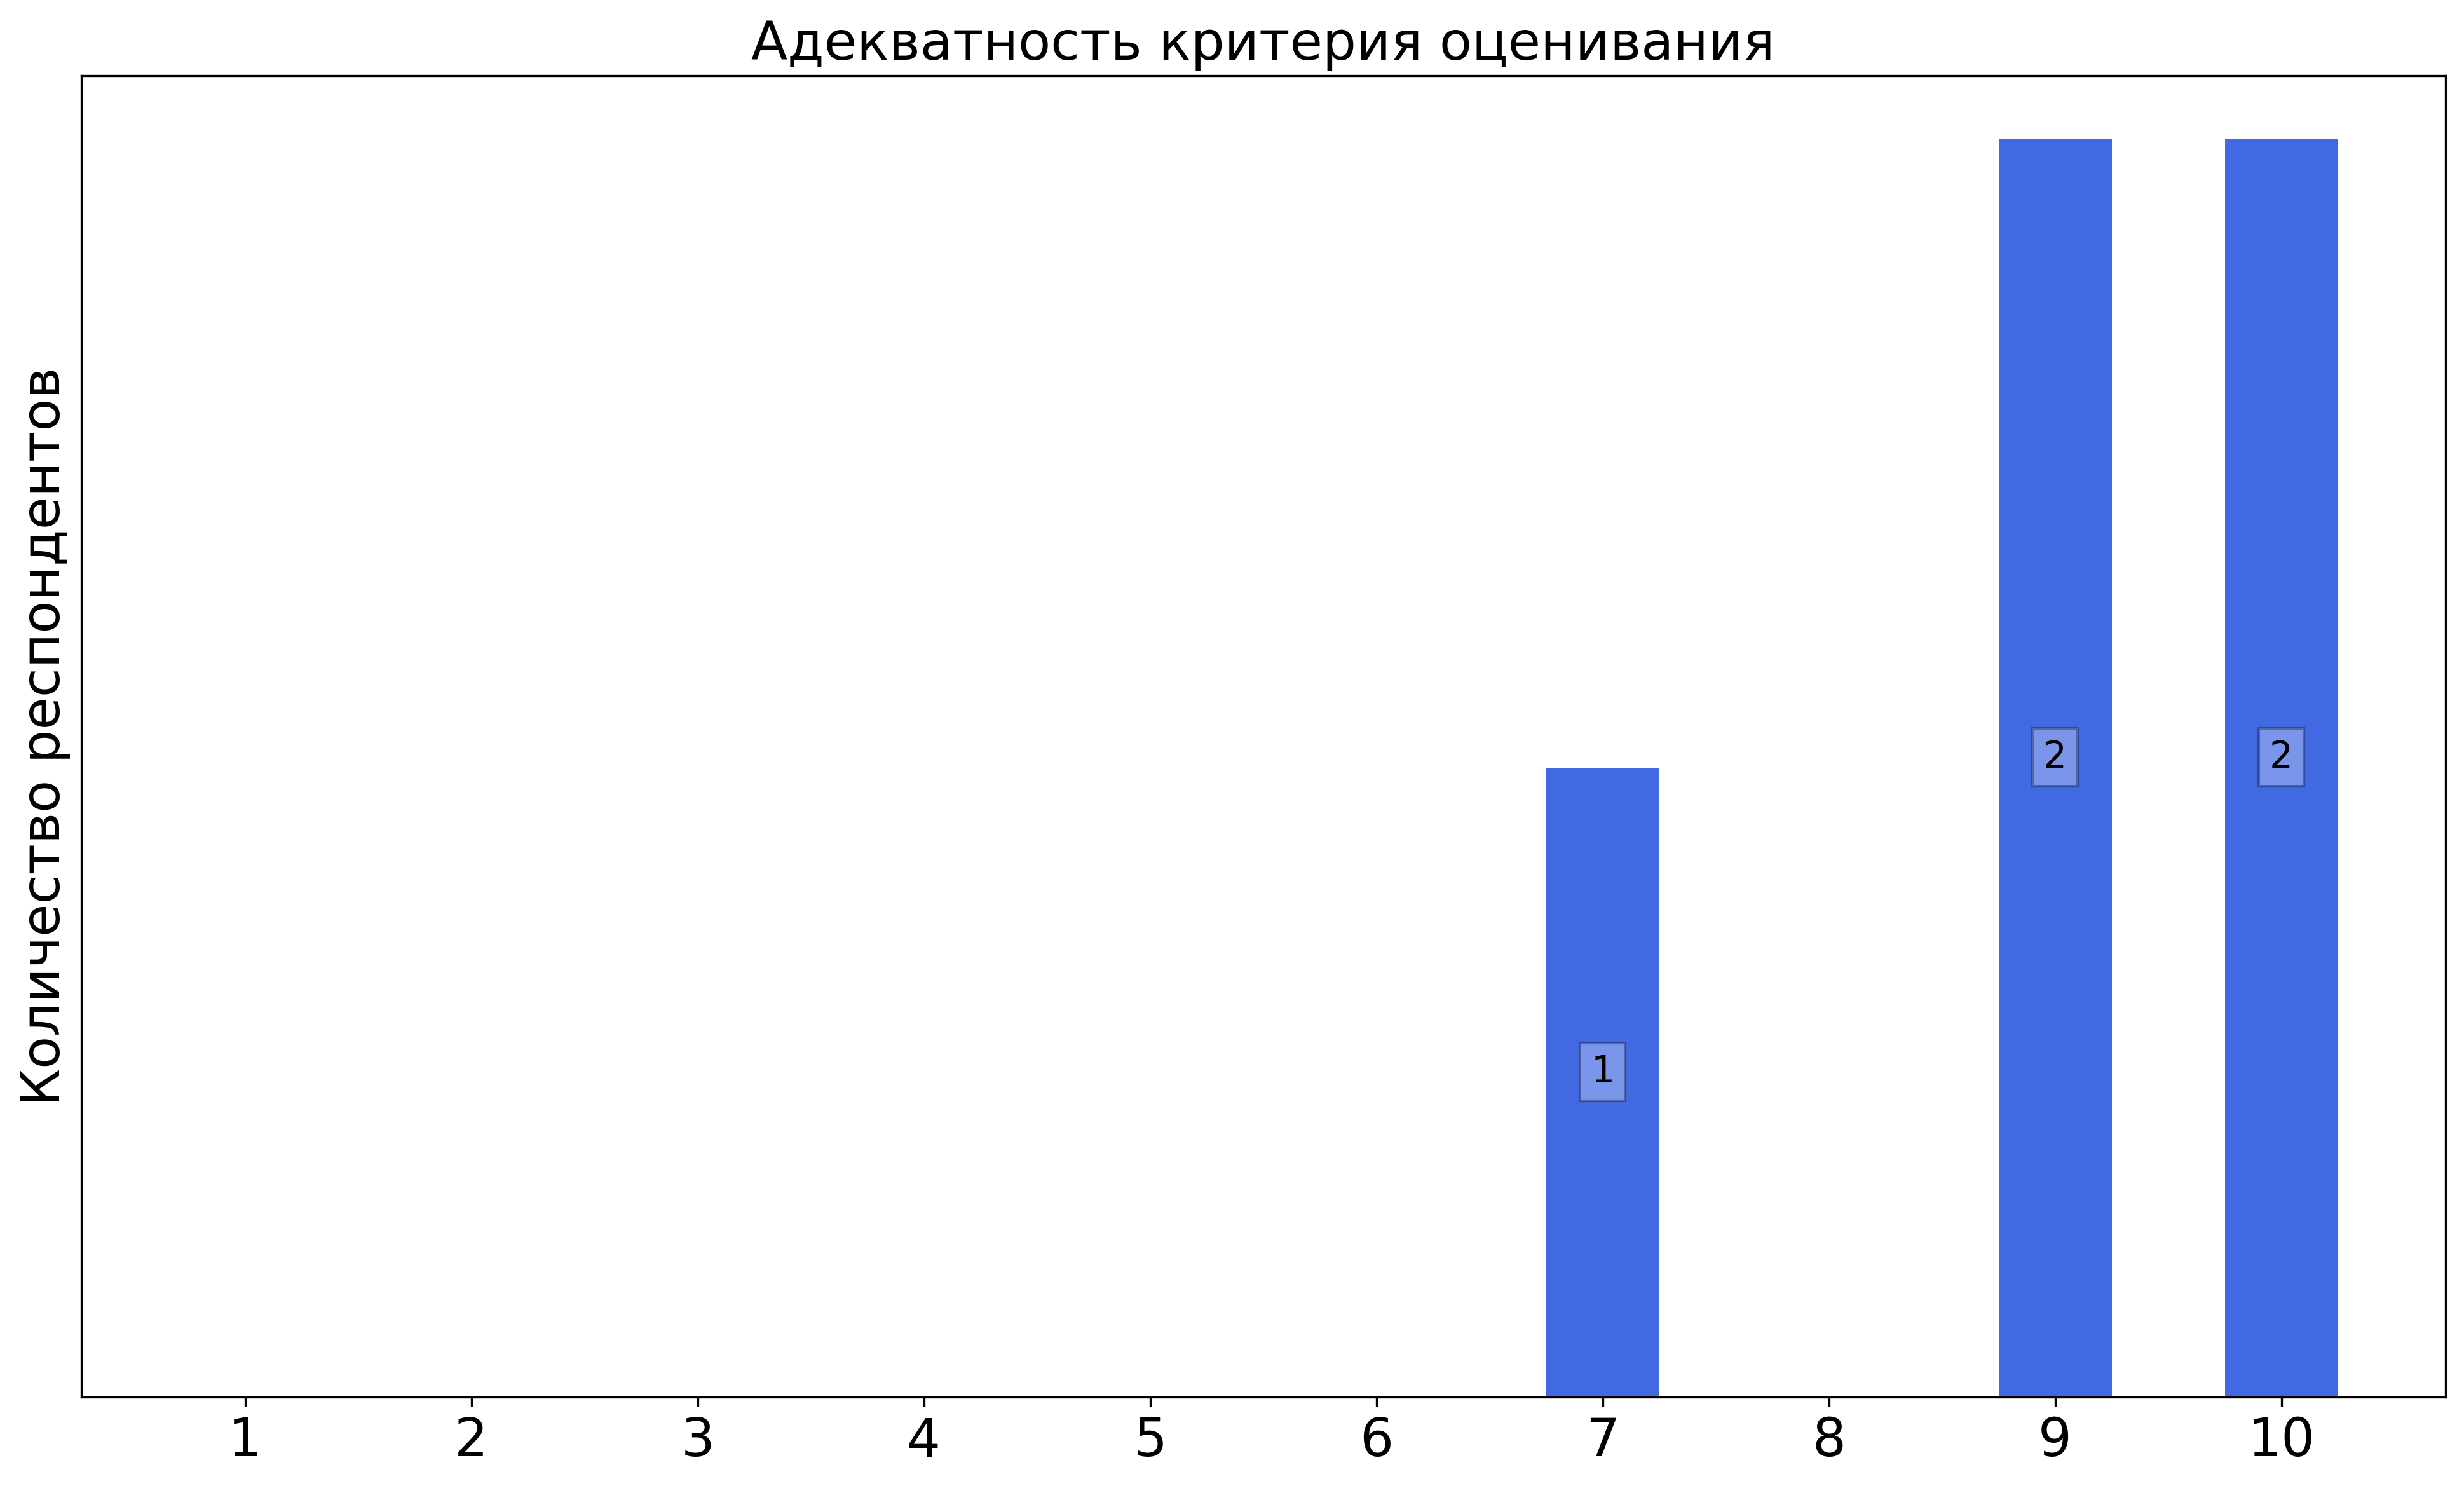
\includegraphics[width=\textwidth]{images/3 course/Общая физика - квантовая физика/labniks-marks-Аникин Ю.А.-1.png}
                \end{subfigure}
                \begin{subfigure}[b]{0.45\textwidth}
                    \centering
                    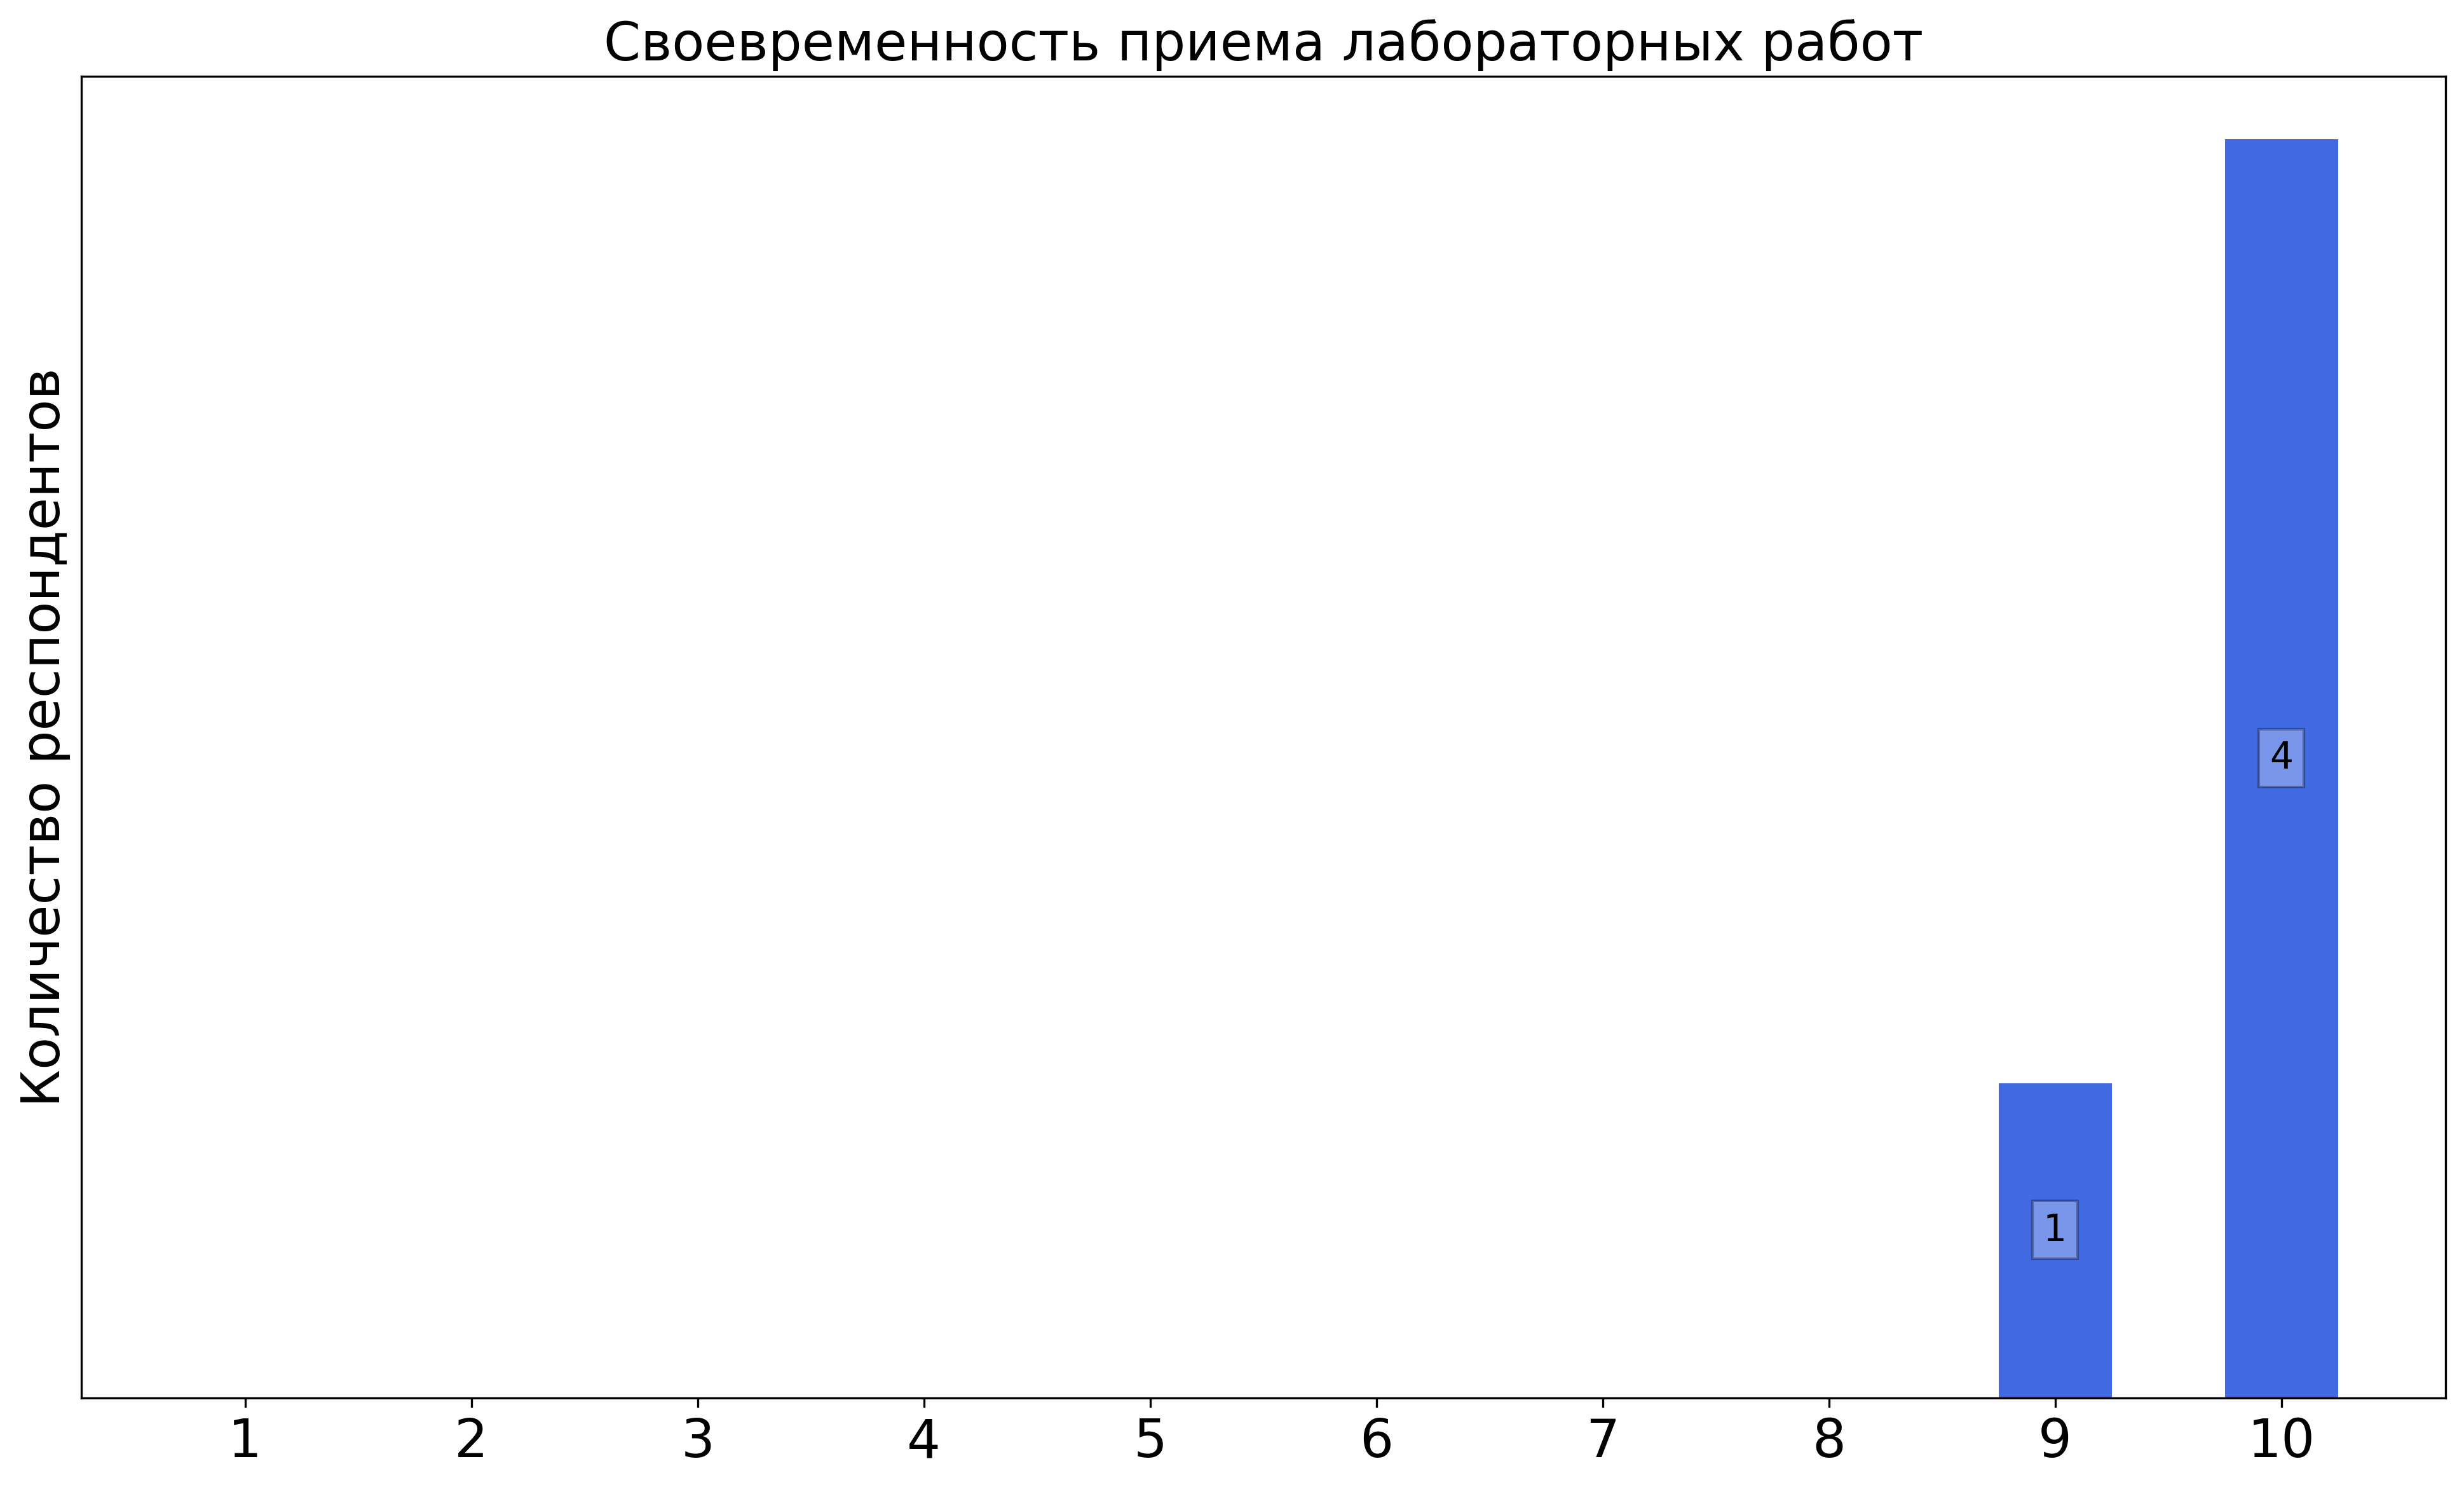
\includegraphics[width=\textwidth]{images/3 course/Общая физика - квантовая физика/labniks-marks-Аникин Ю.А.-2.png}
                \end{subfigure}
                \begin{subfigure}[b]{0.45\textwidth}
                    \centering
                    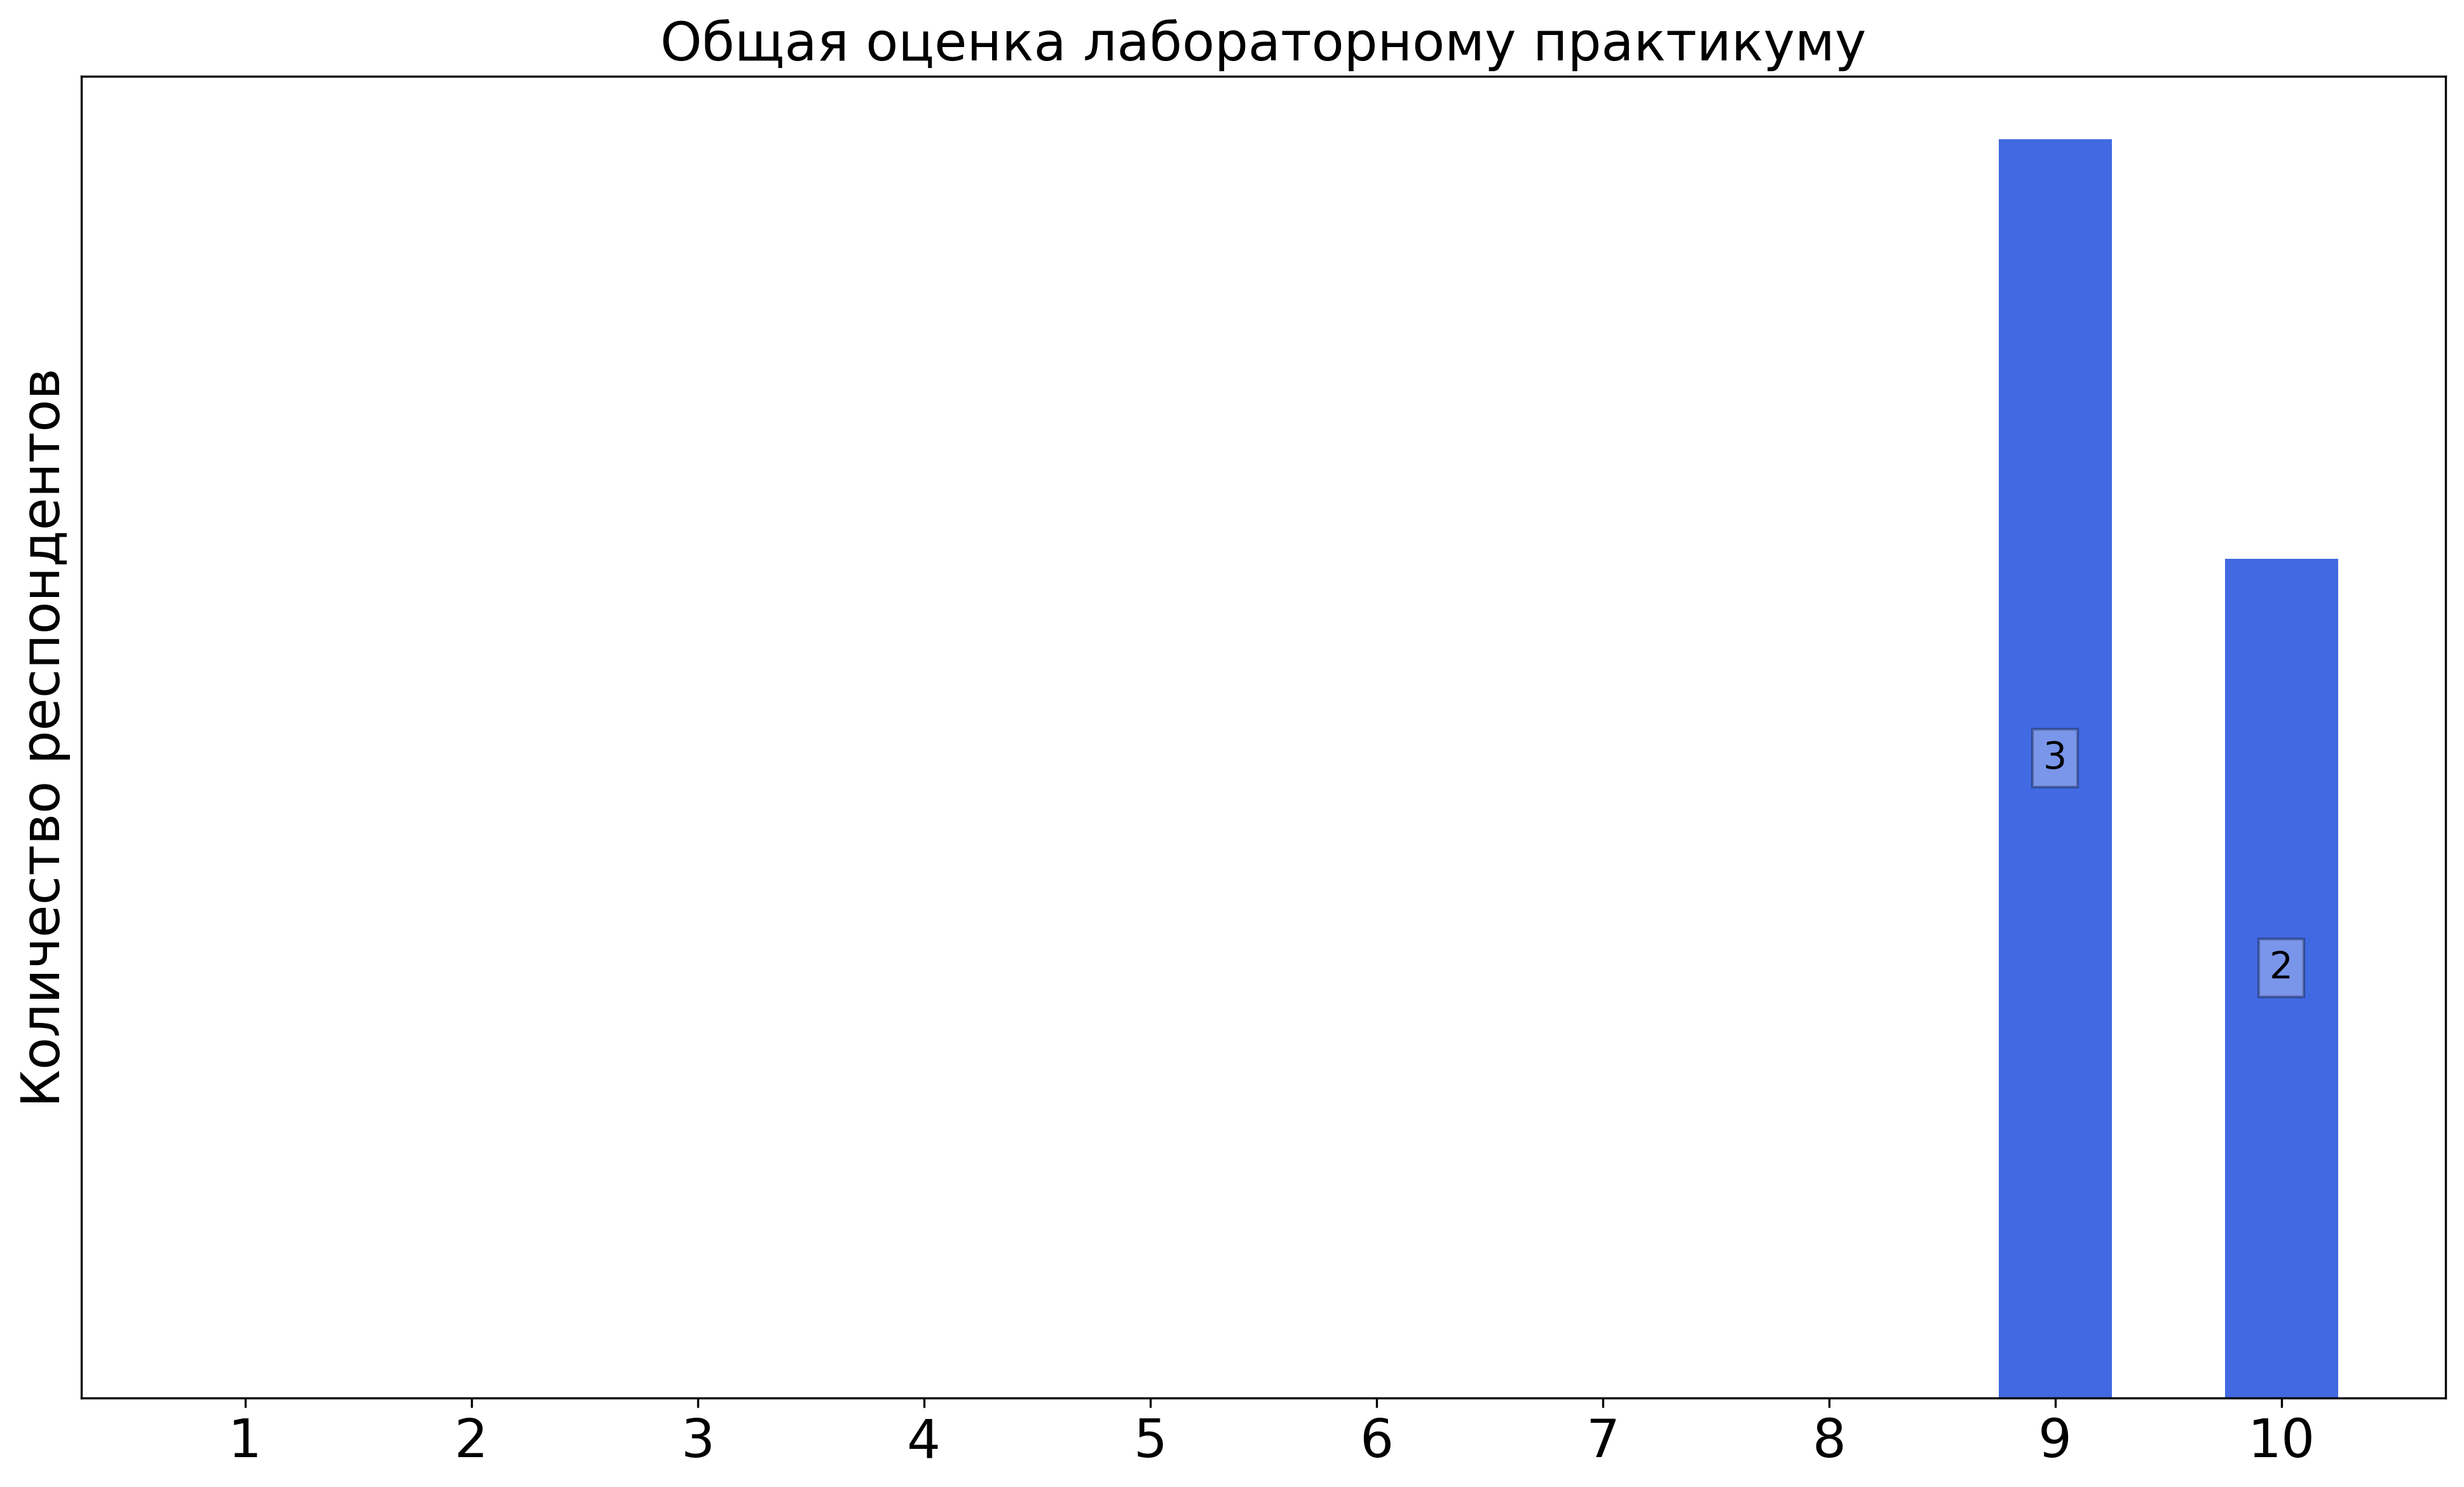
\includegraphics[width=\textwidth]{images/3 course/Общая физика - квантовая физика/labniks-marks-Аникин Ю.А.-3.png}
                \end{subfigure}	
                \caption{Оценки респондентов о качестве преподавания лабораторных работ}
            \end{figure}

            \textbf{Комментарии студентов о преподавателе\protect\footnote{сохранены оригинальные орфография и пунктуация}}
                \begin{commentbox} 
                    Не халява, но лабораторные были интереснын и весёлые с этим преподом 
                \end{commentbox} 
            
                \begin{commentbox} 
                    Перевелся к Архипову, у Аникина был во 2 семестре, знаком довольно хорошо с ним, качество лаб в 5 семестре по моим сведениям было весьма высокое без нереальных требований и с честным оцениванием 
                \end{commentbox}


                
        \subsubsection{Отзыв студентов о лабораторных работах. Преподаватель: Астраханцев Л.}
            \begin{figure}[H]
                \centering
                \begin{subfigure}[b]{0.45\textwidth}
                    \centering
                    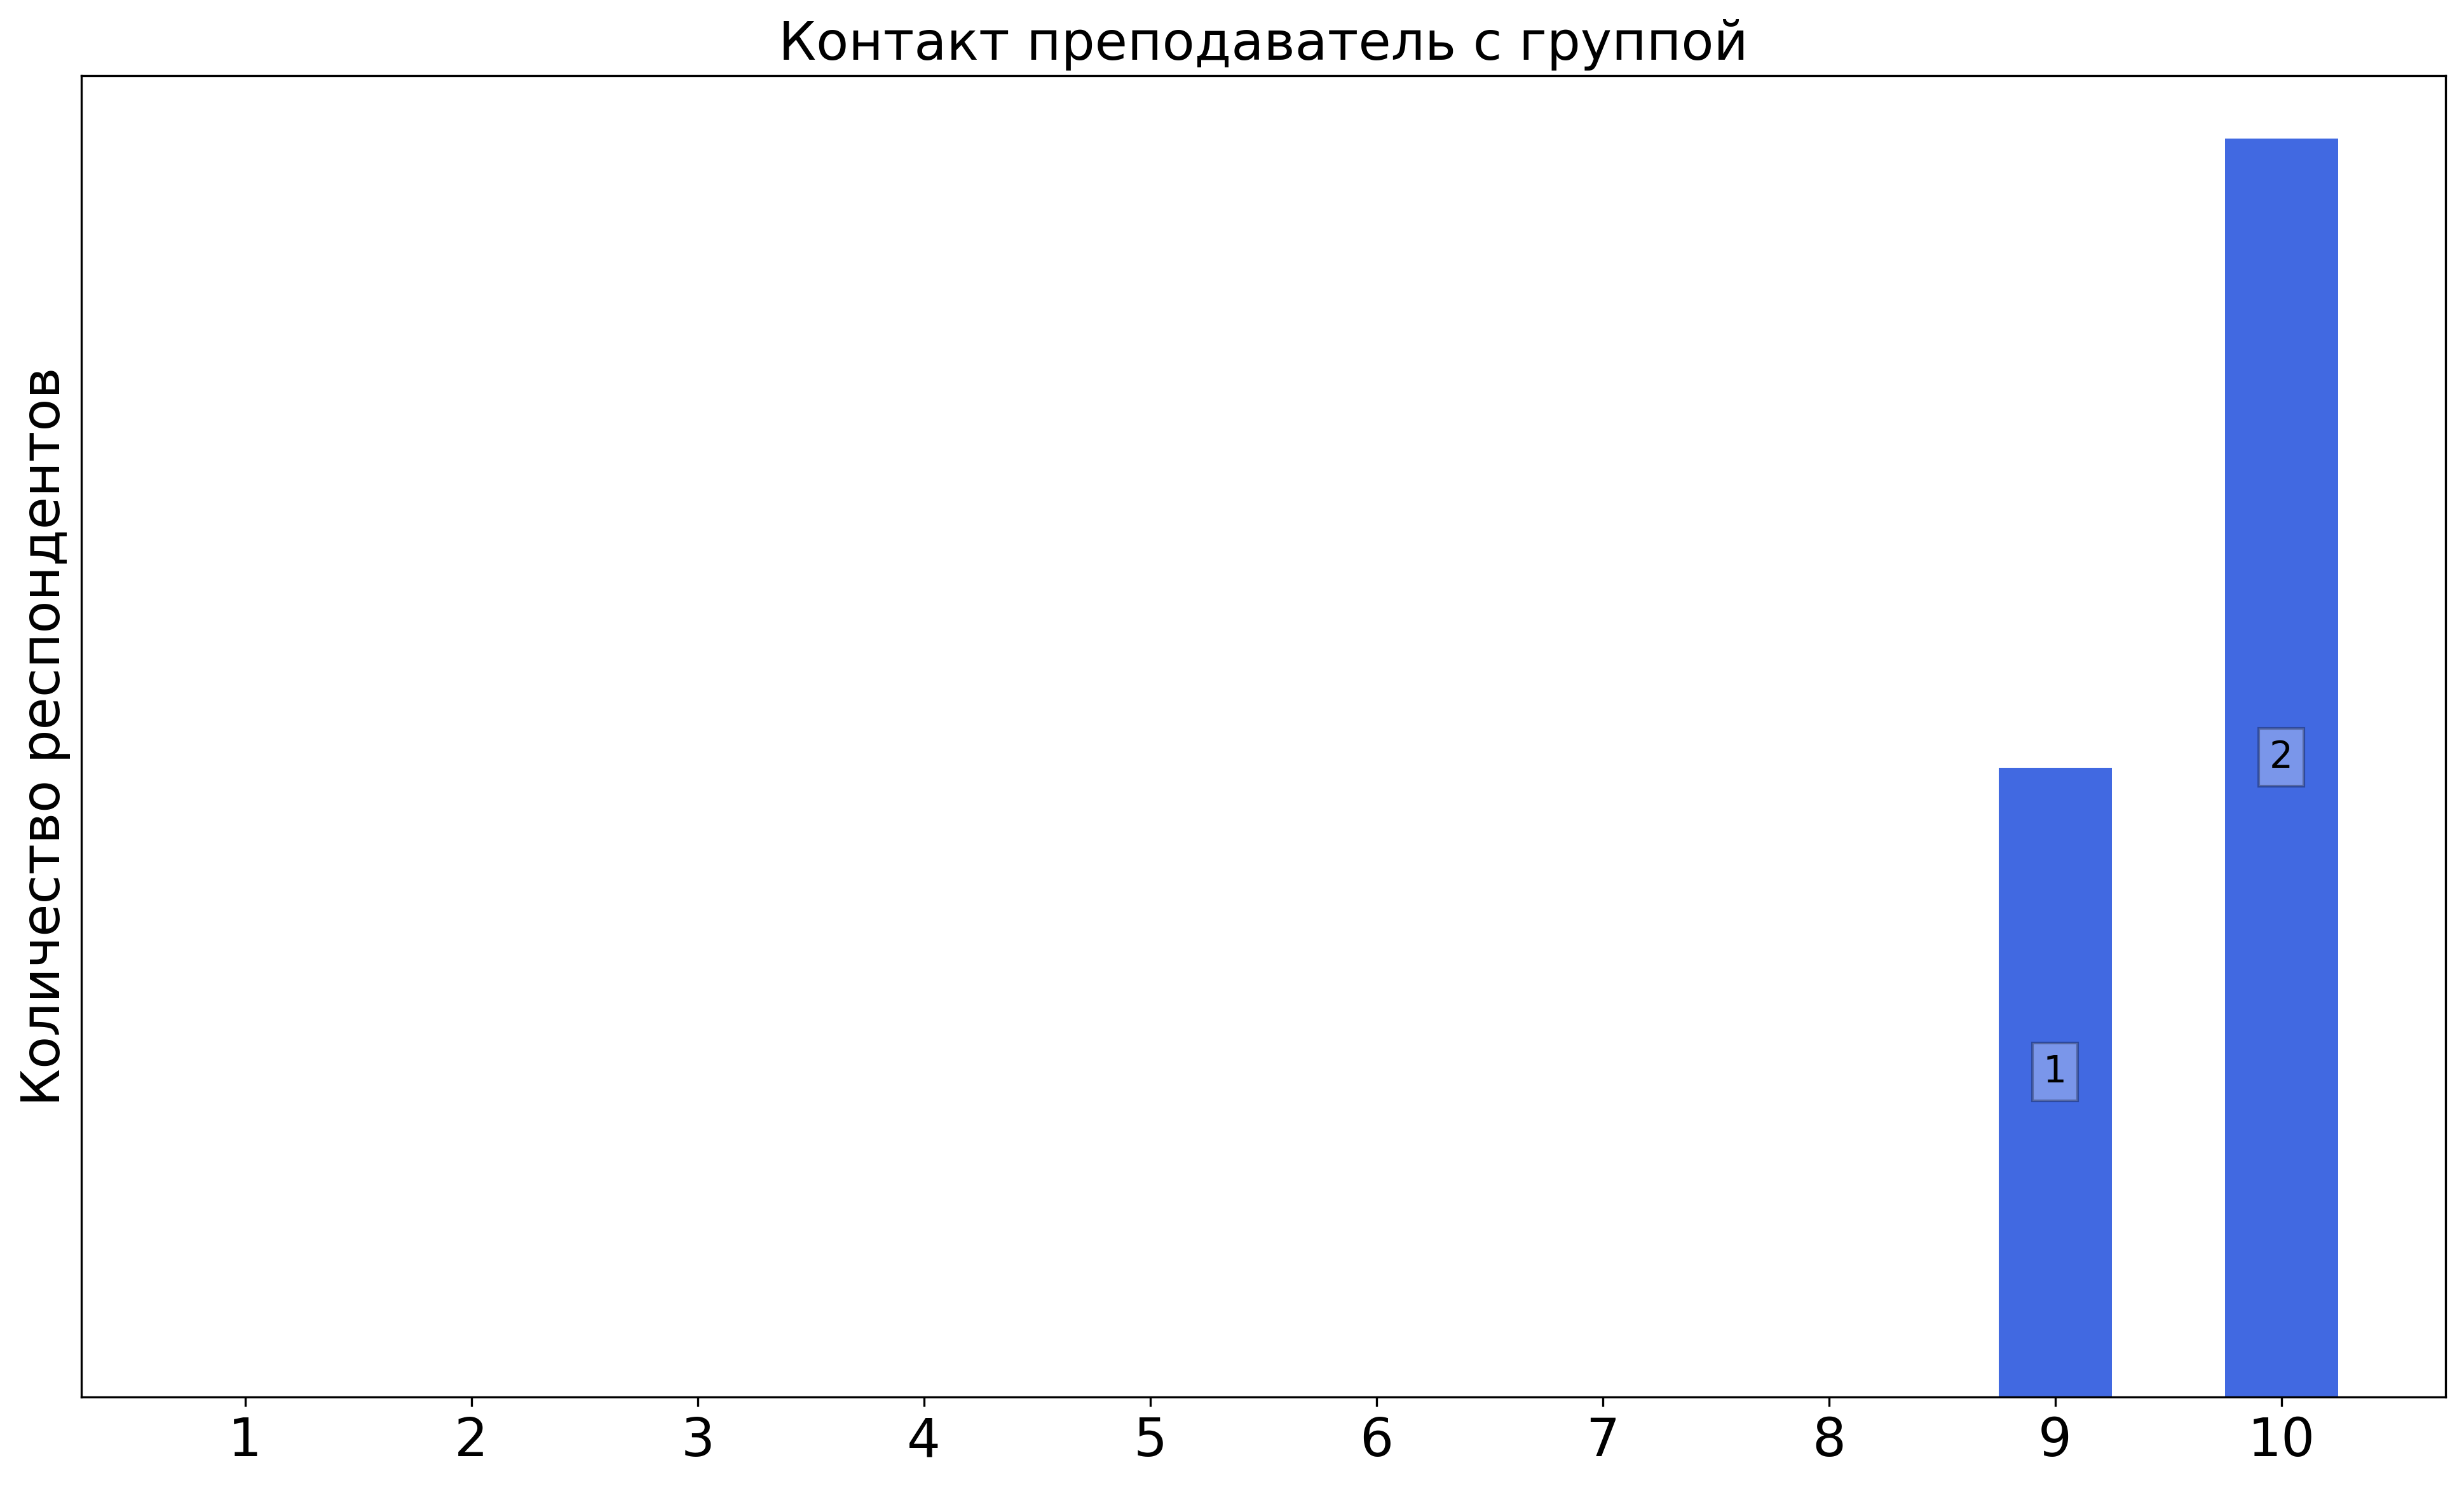
\includegraphics[width=\textwidth]{images/3 course/Общая физика - квантовая физика/labniks-marks-Астраханцев Л.-0.png}
                \end{subfigure}
                \begin{subfigure}[b]{0.45\textwidth}
                    \centering
                    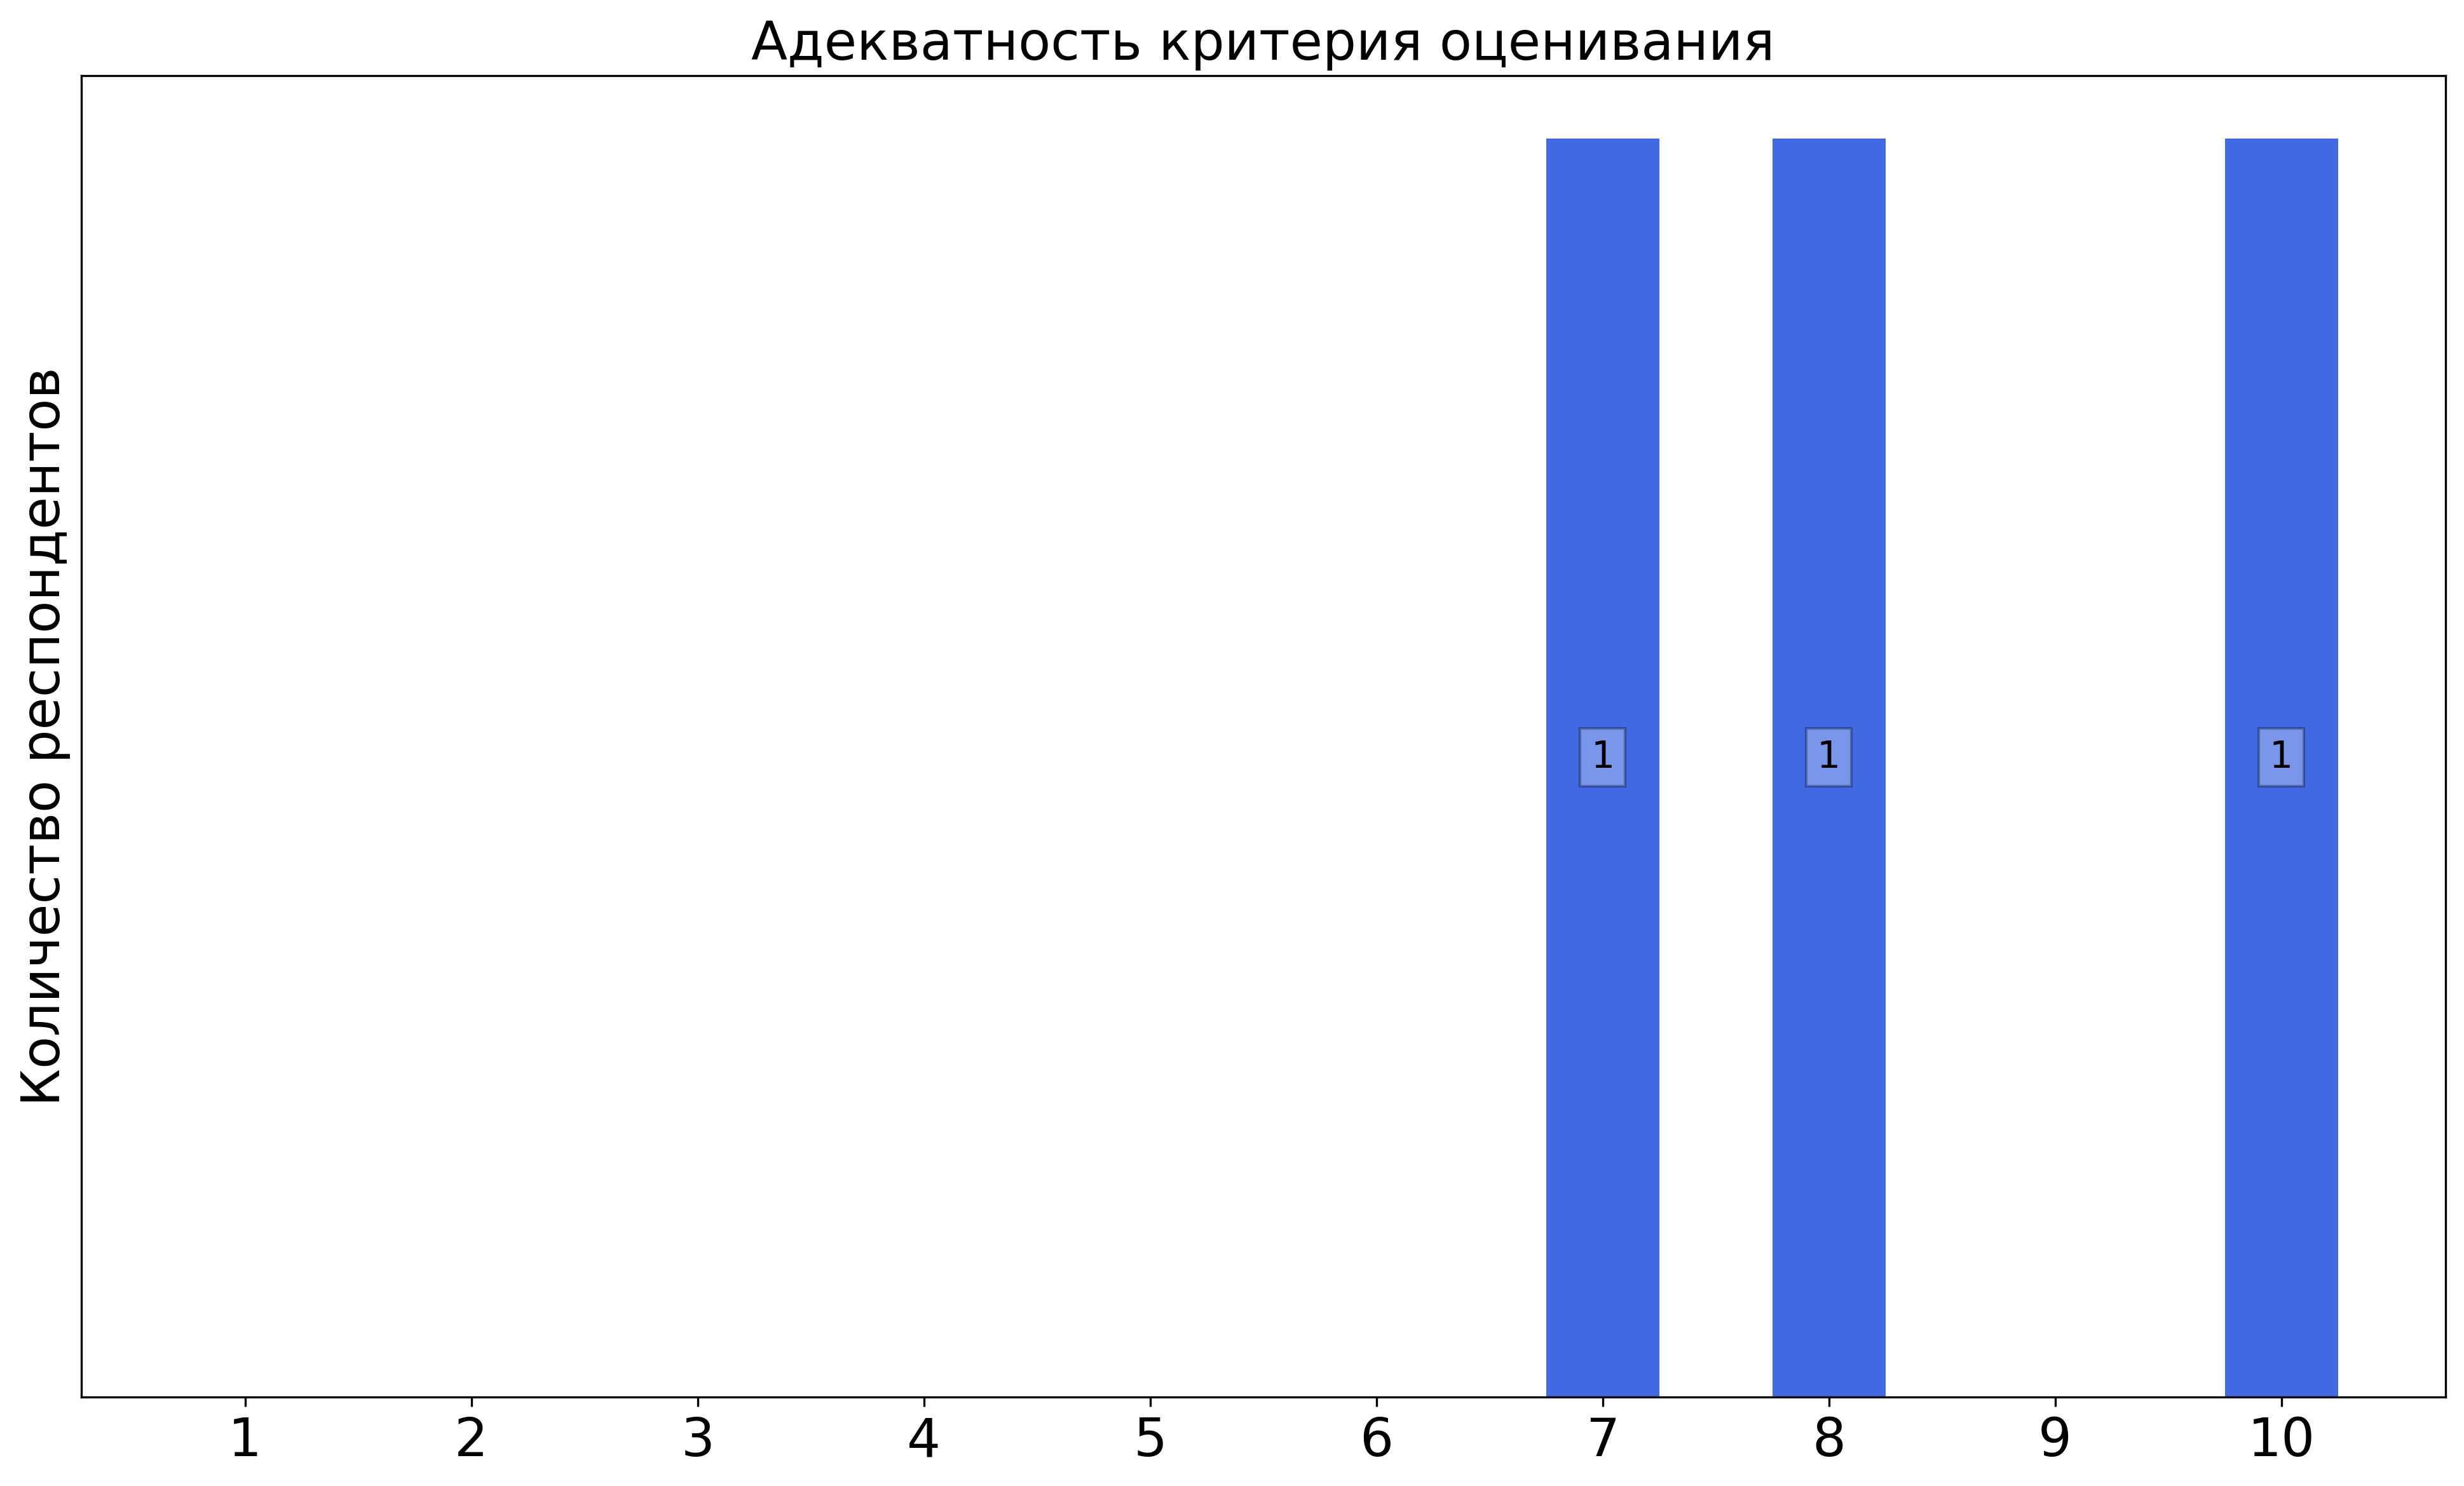
\includegraphics[width=\textwidth]{images/3 course/Общая физика - квантовая физика/labniks-marks-Астраханцев Л.-1.png}
                \end{subfigure}
                \begin{subfigure}[b]{0.45\textwidth}
                    \centering
                    \includegraphics[width=\textwidth]{images/3 course/Общая физика - квантовая физика/labniks-marks-Астраханцев Л.-2.png}
                \end{subfigure}
                \begin{subfigure}[b]{0.45\textwidth}
                    \centering
                    \includegraphics[width=\textwidth]{images/3 course/Общая физика - квантовая физика/labniks-marks-Астраханцев Л.-3.png}
                \end{subfigure}	
                \caption{Оценки респондентов о качестве преподавания лабораторных работ}
            \end{figure}

            \textbf{Комментарии студентов о преподавателе\protect\footnote{сохранены оригинальные орфография и пунктуация}}
                \begin{commentbox} 
                    Все сдачи проходили приятно, объяснял запутанные моменты 
                \end{commentbox}


                
        \subsubsection{Отзыв студентов о лабораторных работах. Преподаватель: Глазков В.Н.}
            \begin{figure}[H]
                \centering
                \begin{subfigure}[b]{0.45\textwidth}
                    \centering
                    \includegraphics[width=\textwidth]{images/3 course/Общая физика - квантовая физика/labniks-marks-Глазков В.Н.-0.png}
                \end{subfigure}
                \begin{subfigure}[b]{0.45\textwidth}
                    \centering
                    \includegraphics[width=\textwidth]{images/3 course/Общая физика - квантовая физика/labniks-marks-Глазков В.Н.-1.png}
                \end{subfigure}
                \begin{subfigure}[b]{0.45\textwidth}
                    \centering
                    \includegraphics[width=\textwidth]{images/3 course/Общая физика - квантовая физика/labniks-marks-Глазков В.Н.-2.png}
                \end{subfigure}
                \begin{subfigure}[b]{0.45\textwidth}
                    \centering
                    \includegraphics[width=\textwidth]{images/3 course/Общая физика - квантовая физика/labniks-marks-Глазков В.Н.-3.png}
                \end{subfigure}	
                \caption{Оценки респондентов о качестве преподавания лабораторных работ}
            \end{figure}

            \textbf{Комментарии студентов о преподавателе\protect\footnote{сохранены оригинальные орфография и пунктуация}}
                \begin{commentbox} 
                    Глазкова В. Н. - великолепин. Ответит на непонятные вопросы по лабе и если попросить, то объяснит сверхпрограммы лабы.  
                \end{commentbox} 

        
                
        \subsubsection{Отзыв студентов о лабораторных работах. Преподаватель: Гуденко С.В.}
            \begin{figure}[H]
                \centering
                \begin{subfigure}[b]{0.45\textwidth}
                    \centering
                    \includegraphics[width=\textwidth]{images/3 course/Общая физика - квантовая физика/labniks-marks-Гуденко С.В.-0.png}
                \end{subfigure}
                \begin{subfigure}[b]{0.45\textwidth}
                    \centering
                    \includegraphics[width=\textwidth]{images/3 course/Общая физика - квантовая физика/labniks-marks-Гуденко С.В.-1.png}
                \end{subfigure}
                \begin{subfigure}[b]{0.45\textwidth}
                    \centering
                    \includegraphics[width=\textwidth]{images/3 course/Общая физика - квантовая физика/labniks-marks-Гуденко С.В.-2.png}
                \end{subfigure}
                \begin{subfigure}[b]{0.45\textwidth}
                    \centering
                    \includegraphics[width=\textwidth]{images/3 course/Общая физика - квантовая физика/labniks-marks-Гуденко С.В.-3.png}
                \end{subfigure}	
                \caption{Оценки респондентов о качестве преподавания лабораторных работ}
            \end{figure}

        
        \subsubsection{Отзыв студентов о лабораторных работах. Преподаватель: Жабин С.Н.}
            \begin{figure}[H]
                \centering
                \begin{subfigure}[b]{0.45\textwidth}
                    \centering
                    \includegraphics[width=\textwidth]{images/3 course/Общая физика - квантовая физика/labniks-marks-Жабин С.Н.-0.png}
                \end{subfigure}
                \begin{subfigure}[b]{0.45\textwidth}
                    \centering
                    \includegraphics[width=\textwidth]{images/3 course/Общая физика - квантовая физика/labniks-marks-Жабин С.Н.-1.png}
                \end{subfigure}
                \begin{subfigure}[b]{0.45\textwidth}
                    \centering
                    \includegraphics[width=\textwidth]{images/3 course/Общая физика - квантовая физика/labniks-marks-Жабин С.Н.-2.png}
                \end{subfigure}
                \begin{subfigure}[b]{0.45\textwidth}
                    \centering
                    \includegraphics[width=\textwidth]{images/3 course/Общая физика - квантовая физика/labniks-marks-Жабин С.Н.-3.png}
                \end{subfigure}	
                \caption{Оценки респондентов о качестве преподавания лабораторных работ}
            \end{figure}

            \textbf{Комментарии студентов о преподавателе\protect\footnote{сохранены оригинальные орфография и пунктуация}}
                \begin{commentbox} 
                    Очень интересный человек и преподаватель, пытается донести всем главную суть. Достаточно халявный, в конце просто так повысил оценку 
                \end{commentbox} 
            
                \begin{commentbox} 
                    Часто опаздывал на занятия, на 1.5-2 часа. Контакт вроде через телеграмм был, но в основном не отвечал 
                \end{commentbox}

            
            
        \subsubsection{Отзыв студентов о лабораторных работах. Преподаватель: Зубович Н.Ю.}
            \begin{figure}[H]
                \centering
                \begin{subfigure}[b]{0.45\textwidth}
                    \centering
                    \includegraphics[width=\textwidth]{images/3 course/Общая физика - квантовая физика/labniks-marks-Зубович Н.Ю.-0.png}
                \end{subfigure}
                \begin{subfigure}[b]{0.45\textwidth}
                    \centering
                    \includegraphics[width=\textwidth]{images/3 course/Общая физика - квантовая физика/labniks-marks-Зубович Н.Ю.-1.png}
                \end{subfigure}
                \begin{subfigure}[b]{0.45\textwidth}
                    \centering
                    \includegraphics[width=\textwidth]{images/3 course/Общая физика - квантовая физика/labniks-marks-Зубович Н.Ю.-2.png}
                \end{subfigure}
                \begin{subfigure}[b]{0.45\textwidth}
                    \centering
                    \includegraphics[width=\textwidth]{images/3 course/Общая физика - квантовая физика/labniks-marks-Зубович Н.Ю.-3.png}
                \end{subfigure}	
                \caption{Оценки респондентов о качестве преподавания лабораторных работ}
            \end{figure}

            \textbf{Комментарии студентов о преподавателе\protect\footnote{сохранены оригинальные орфография и пунктуация}}
                \begin{commentbox} 
                    Спасибо большое Наталье Юрьевне за этот курс лабораторных работ. Самая лучший преподаватель по лабам за все 5 семестров. Сдачи и выполнения проходили крайне увлекательно. Обсуждали вместе теорию и установку во время выполнения, а на сдаче все вместе по очереди рассказывали о результатах, кто-то делал доклады об ученых или интересных явлениях в квантовой физике. Благодаря Наталье Юрьевне остались отличные знания в области квантовой физики. 
                \end{commentbox} 
            
                \begin{commentbox} 
                    Сами лабы прикольные, хотя мозги взрывают. Зубович лабник хороший. Сразу запоминает всех студентов, ко всем относится с уважением. При этом предмет свой знает и требует на базовом уровне этого и от студентов. Лабы принимаются легко, больше похоже на обсуждение теории, в конце которой всем ставит отлы 
                \end{commentbox}


        \subsubsection{Отзыв студентов о лабораторных работах. Преподаватель: Инжечик Л.В.}
            \begin{figure}[H]
                \centering
                \begin{subfigure}[b]{0.45\textwidth}
                    \centering
                    \includegraphics[width=\textwidth]{images/3 course/Общая физика - квантовая физика/labniks-marks-Инжечик Л.В.-0.png}
                \end{subfigure}
                \begin{subfigure}[b]{0.45\textwidth}
                    \centering
                    \includegraphics[width=\textwidth]{images/3 course/Общая физика - квантовая физика/labniks-marks-Инжечик Л.В.-1.png}
                \end{subfigure}
                \begin{subfigure}[b]{0.45\textwidth}
                    \centering
                    \includegraphics[width=\textwidth]{images/3 course/Общая физика - квантовая физика/labniks-marks-Инжечик Л.В.-2.png}
                \end{subfigure}
                \begin{subfigure}[b]{0.45\textwidth}
                    \centering
                    \includegraphics[width=\textwidth]{images/3 course/Общая физика - квантовая физика/labniks-marks-Инжечик Л.В.-3.png}
                \end{subfigure}	
                \caption{Оценки респондентов о качестве преподавания лабораторных работ}
            \end{figure}


            
        \subsubsection{Отзыв студентов о лабораторных работах. Преподаватель: Колдунов М.Ф.}
            \begin{figure}[H]
                \centering
                \begin{subfigure}[b]{0.45\textwidth}
                    \centering
                    \includegraphics[width=\textwidth]{images/3 course/Общая физика - квантовая физика/labniks-marks-Колдунов М.Ф.-0.png}
                \end{subfigure}
                \begin{subfigure}[b]{0.45\textwidth}
                    \centering
                    \includegraphics[width=\textwidth]{images/3 course/Общая физика - квантовая физика/labniks-marks-Колдунов М.Ф.-1.png}
                \end{subfigure}
                \begin{subfigure}[b]{0.45\textwidth}
                    \centering
                    \includegraphics[width=\textwidth]{images/3 course/Общая физика - квантовая физика/labniks-marks-Колдунов М.Ф.-2.png}
                \end{subfigure}
                \begin{subfigure}[b]{0.45\textwidth}
                    \centering
                    \includegraphics[width=\textwidth]{images/3 course/Общая физика - квантовая физика/labniks-marks-Колдунов М.Ф.-3.png}
                \end{subfigure}	
                \caption{Оценки респондентов о качестве преподавания лабораторных работ}
            \end{figure}

            \textbf{Комментарии студентов о преподавателе\protect\footnote{сохранены оригинальные орфография и пунктуация}}
                \begin{commentbox} 
                    Интересный опыт конечно, каждая сдача - беседа по всему разделу и самой лабе. Знать нужно все, чтобы хотя бы один человек из группы мог ответить на вопрос. Отчет не важен, но должен быть написан на бумаге. Оценка ставится как бы всей группе (коллективная ответственность, по словам самого преподавателя) в зависимости от того как много и по делу ты говорил. Если готовиться, оценки ставятся очень щедрые. 
                \end{commentbox}

        
        \subsubsection{Отзыв студентов о лабораторных работах. Преподаватель: Почернин И.Г.}
            \begin{figure}[H]
                \centering
                \begin{subfigure}[b]{0.45\textwidth}
                    \centering
                    \includegraphics[width=\textwidth]{images/3 course/Общая физика - квантовая физика/labniks-marks-Почернин И.Г.-0.png}
                \end{subfigure}
                \begin{subfigure}[b]{0.45\textwidth}
                    \centering
                    \includegraphics[width=\textwidth]{images/3 course/Общая физика - квантовая физика/labniks-marks-Почернин И.Г.-1.png}
                \end{subfigure}
                \begin{subfigure}[b]{0.45\textwidth}
                    \centering
                    \includegraphics[width=\textwidth]{images/3 course/Общая физика - квантовая физика/labniks-marks-Почернин И.Г.-2.png}
                \end{subfigure}
                \begin{subfigure}[b]{0.45\textwidth}
                    \centering
                    \includegraphics[width=\textwidth]{images/3 course/Общая физика - квантовая физика/labniks-marks-Почернин И.Г.-3.png}
                \end{subfigure}	
                \caption{Оценки респондентов о качестве преподавания лабораторных работ}
            \end{figure}

            \textbf{Комментарии студентов о преподавателе\protect\footnote{сохранены оригинальные орфография и пунктуация}}
                \begin{commentbox} 
                    Лабы прошли мимо меня. Опять же, я сам не был сильно заинтересован в этом предмете. Грубо говоря, ботал просто для "джентельменского набора".
                \end{commentbox}


        
        \subsubsection{Отзыв студентов о лабораторных работах. Преподаватель: Салмин В.В.}
            \begin{figure}[H]
                \centering
                \begin{subfigure}[b]{0.45\textwidth}
                    \centering
                    \includegraphics[width=\textwidth]{images/3 course/Общая физика - квантовая физика/labniks-marks-Салмин В.В.-0.png}
                \end{subfigure}
                \begin{subfigure}[b]{0.45\textwidth}
                    \centering
                    \includegraphics[width=\textwidth]{images/3 course/Общая физика - квантовая физика/labniks-marks-Салмин В.В.-1.png}
                \end{subfigure}
                \begin{subfigure}[b]{0.45\textwidth}
                    \centering
                    \includegraphics[width=\textwidth]{images/3 course/Общая физика - квантовая физика/labniks-marks-Салмин В.В.-2.png}
                \end{subfigure}
                \begin{subfigure}[b]{0.45\textwidth}
                    \centering
                    \includegraphics[width=\textwidth]{images/3 course/Общая физика - квантовая физика/labniks-marks-Салмин В.В.-3.png}
                \end{subfigure}	
                \caption{Оценки респондентов о качестве преподавания лабораторных работ}
            \end{figure}

            \textbf{Комментарии студентов о преподавателе\protect\footnote{сохранены оригинальные орфография и пунктуация}}  
                \begin{commentbox} 
                    Не понимал, почему нас так гоняют по теории, но к ГОСу я всё понял... 
                \end{commentbox} 

                \begin{commentbox} 
                    Курс очень интересный, но у моего лабника были достаточно странные критерии оценивания. Он почти не спрашивал теорию, но зато прямо на сдаче мы исправляли его замечания по поводу обработки данных, графиков и тд. Не скажу, что это было действительно полезно для понимания курса физики 
                \end{commentbox} 

                \begin{commentbox} 
                    Очень интересный преподаватель. За семестр научит правильно оформлять отчёт и обрабатывать данные так, если бы вы писали какую-нибудь научную работу. Требует автоматизировать измерения там, где это возможно (например, оцифровка фото осциллограммы, т.к. в ЛК стоят старые осциллографы без возможности записи на флешку), причём Салмин вам с удовольствием пояснит, почему лучше делать именно так. Позволяет править отчеты прямо на сдаче, что является большим плюсом. 
                \end{commentbox}


                
        \subsubsection{Отзыв студентов о лабораторных работах. Преподаватель: Сафонов А.И.}
            \begin{figure}[H]
                \centering
                \begin{subfigure}[b]{0.45\textwidth}
                    \centering
                    \includegraphics[width=\textwidth]{images/3 course/Общая физика - квантовая физика/labniks-marks-Сафонов А.И.-0.png}
                \end{subfigure}
                \begin{subfigure}[b]{0.45\textwidth}
                    \centering
                    \includegraphics[width=\textwidth]{images/3 course/Общая физика - квантовая физика/labniks-marks-Сафонов А.И.-1.png}
                \end{subfigure}
                \begin{subfigure}[b]{0.45\textwidth}
                    \centering
                    \includegraphics[width=\textwidth]{images/3 course/Общая физика - квантовая физика/labniks-marks-Сафонов А.И.-2.png}
                \end{subfigure}
                \begin{subfigure}[b]{0.45\textwidth}
                    \centering
                    \includegraphics[width=\textwidth]{images/3 course/Общая физика - квантовая физика/labniks-marks-Сафонов А.И.-3.png}
                \end{subfigure}	
                \caption{Оценки респондентов о качестве преподавания лабораторных работ}
            \end{figure}

            \textbf{Комментарии студентов о преподавателе\protect\footnote{сохранены оригинальные орфография и пунктуация}}
                \begin{commentbox} 
                    Довольно жесткий лабник. Невероятно умный, чего и требует от других. Принимает достаточно жестко. Не любит ставить удовлетворительно, поэтому отправляет иногда студентов доучивать материал. Отчет смотрит внимательно, особенно графики  
                \end{commentbox}

        
        \subsubsection{Отзыв студентов о лабораторных работах. Преподаватель: Стожков В.Ю.}
            \begin{figure}[H]
                \centering
                \begin{subfigure}[b]{0.45\textwidth}
                    \centering
                    \includegraphics[width=\textwidth]{images/3 course/Общая физика - квантовая физика/labniks-marks-Стожков В.Ю.-0.png}
                \end{subfigure}
                \begin{subfigure}[b]{0.45\textwidth}
                    \centering
                    \includegraphics[width=\textwidth]{images/3 course/Общая физика - квантовая физика/labniks-marks-Стожков В.Ю.-1.png}
                \end{subfigure}
                \begin{subfigure}[b]{0.45\textwidth}
                    \centering
                    \includegraphics[width=\textwidth]{images/3 course/Общая физика - квантовая физика/labniks-marks-Стожков В.Ю.-2.png}
                \end{subfigure}
                \begin{subfigure}[b]{0.45\textwidth}
                    \centering
                    \includegraphics[width=\textwidth]{images/3 course/Общая физика - квантовая физика/labniks-marks-Стожков В.Ю.-3.png}
                \end{subfigure}	
                \caption{Оценки респондентов о качестве преподавания лабораторных работ}
            \end{figure}

            \textbf{Комментарии студентов о преподавателе\protect\footnote{сохранены оригинальные орфография и пунктуация}}
                \begin{commentbox} 
                    Стожков Владимир Юрьевич прекрасен. Вот так, наверное, и должны вестись лабораторные работы. Небольшая беседа перед выполнением, и много обсуждений во время сдачи. Очень приятный. 10/10. К тому же и принимает довольно лояльно, если придерживаться дисциплины. 
                \end{commentbox}


        \subsubsection{Отзыв студентов о лабораторных работах. Преподаватель: Судаков О.А.}
            \begin{figure}[H]
                \centering
                \begin{subfigure}[b]{0.45\textwidth}
                    \centering
                    \includegraphics[width=\textwidth]{images/3 course/Общая физика - квантовая физика/labniks-marks-Судаков О.А.-0.png}
                \end{subfigure}
                \begin{subfigure}[b]{0.45\textwidth}
                    \centering
                    \includegraphics[width=\textwidth]{images/3 course/Общая физика - квантовая физика/labniks-marks-Судаков О.А.-1.png}
                \end{subfigure}
                \begin{subfigure}[b]{0.45\textwidth}
                    \centering
                    \includegraphics[width=\textwidth]{images/3 course/Общая физика - квантовая физика/labniks-marks-Судаков О.А.-2.png}
                \end{subfigure}
                \begin{subfigure}[b]{0.45\textwidth}
                    \centering
                    \includegraphics[width=\textwidth]{images/3 course/Общая физика - квантовая физика/labniks-marks-Судаков О.А.-3.png}
                \end{subfigure}	
                \caption{Оценки респондентов о качестве преподавания лабораторных работ}
            \end{figure}

            \textbf{Комментарии студентов о преподавателе\protect\footnote{сохранены оригинальные орфография и пунктуация}}
                \begin{commentbox} 
                    Лабник помогал при выполнении, шёл часто на встречу и оценивал в целом адекватно.  
                \end{commentbox} 
            
                \begin{commentbox} 
                    Довольно странные "загадки" на сдаче. 
                \end{commentbox}

                
        \subsubsection{Отзыв студентов о лабораторных работах. Преподаватель: Хан Ф.В.}
            \begin{figure}[H]
                \centering
                \begin{subfigure}[b]{0.45\textwidth}
                    \centering
                    \includegraphics[width=\textwidth]{images/3 course/Общая физика - квантовая физика/labniks-marks-Хан Ф.В.-0.png}
                \end{subfigure}
                \begin{subfigure}[b]{0.45\textwidth}
                    \centering
                    \includegraphics[width=\textwidth]{images/3 course/Общая физика - квантовая физика/labniks-marks-Хан Ф.В.-1.png}
                \end{subfigure}
                \begin{subfigure}[b]{0.45\textwidth}
                    \centering
                    \includegraphics[width=\textwidth]{images/3 course/Общая физика - квантовая физика/labniks-marks-Хан Ф.В.-2.png}
                \end{subfigure}
                \begin{subfigure}[b]{0.45\textwidth}
                    \centering
                    \includegraphics[width=\textwidth]{images/3 course/Общая физика - квантовая физика/labniks-marks-Хан Ф.В.-3.png}
                \end{subfigure}	
                \caption{Оценки респондентов о качестве преподавания лабораторных работ}
            \end{figure}

            \textbf{Комментарии студентов о преподавателе\protect\footnote{сохранены оригинальные орфография и пунктуация}}
                \begin{commentbox} 
                    Один из лучших лабников за все семестры - отлично расшаривается теория на совместном обсуждении на сдаче, всегда поможет понять лабу. Старается выглядеть строго. Сдачи очень долгие, обычно после 2х пар ещё задерживаемся на перемене. Оценки выставил очень приятные, несмотря на тяжелые сдачи. В лабах смотрел на адекватность и давал общие рекомендации, не забивал на отчет, учил его правильнее оформлять, но при этом не докапывался до погрешностей или того, где и как построен график - в общем, образцовый преподаватель кафедры общей физики. Единственное, что грустно - лабы с 9 утра - думать нереально  
                \end{commentbox} 
            
                \begin{commentbox} 
                    Отличный лабник, который вкладывается в работу, целью ставит усвоение студентами материала, развитие более глубокого понимания предмета. Перед лабой и во время сдачи обсуждается много теории, что хорошо сказывается на прохождении курса. Основной сложностью была сдача отчета, так как приходилось переделывать и пересылать по нескольку раз, если что-то его не устраивало, но это мелочи по сравнению с количеством и качеством пройденного материала. 
                \end{commentbox} 


        \subsubsection{Отзыв студентов о лабораторных работах. Преподаватель: Юрьев Ю.В.}
            \begin{figure}[H]
                \centering
                \begin{subfigure}[b]{0.45\textwidth}
                    \centering
                    \includegraphics[width=\textwidth]{images/3 course/Общая физика - квантовая физика/labniks-marks-Юрьев Ю.В.-0.png}
                \end{subfigure}
                \begin{subfigure}[b]{0.45\textwidth}
                    \centering
                    \includegraphics[width=\textwidth]{images/3 course/Общая физика - квантовая физика/labniks-marks-Юрьев Ю.В.-1.png}
                \end{subfigure}
                \begin{subfigure}[b]{0.45\textwidth}
                    \centering
                    \includegraphics[width=\textwidth]{images/3 course/Общая физика - квантовая физика/labniks-marks-Юрьев Ю.В.-2.png}
                \end{subfigure}
                \begin{subfigure}[b]{0.45\textwidth}
                    \centering
                    \includegraphics[width=\textwidth]{images/3 course/Общая физика - квантовая физика/labniks-marks-Юрьев Ю.В.-3.png}
                \end{subfigure}	
                \caption{Оценки респондентов о качестве преподавания лабораторных работ}
            \end{figure}

            \textbf{Комментарии студентов о преподавателе\protect\footnote{сохранены оригинальные орфография и пунктуация}}
                \begin{commentbox} 
                    Очень лоялен 
                \end{commentbox} 
            
                \begin{commentbox} 
                    Исключительно положительные эмоции. Сдачи длятся всегда все 2 пары, но выглядят в виде несложных задачек и разбора теории, где Юрий Вячеславович периодически уходит в ответы на всевозможные наши вопросы (по тонкостям работы, а иногда и по самой базе). Рассказывает понятно и действительно интересно. Честно, я б даже ему роль лектора предложил 
                \end{commentbox} 
            
                \begin{commentbox} 
                    Самый лучший лабник, все ушли с хорошими оценками и знаниями (сдачи лабораторных работ много чему научили) 
                \end{commentbox} 
            
                \begin{commentbox} 
                    Держит в аудитории все две пары, в это время рассказывает теорию и спрашивает насущные вопросы. Оценивает неадекватно лояльно, но это даже мотивирует разбираться в материале, ведь оценка в любом случае будет хорошей, а разочаровывать Юрьева совсем не хочет, ведь он всем видом показывает, что хочет научить и верит в нас. Приятный преподаватель. Так же один из самый хороших семестров по физлабам  
                \end{commentbox} 
            
                \begin{commentbox} 
                    Лучший лабник на кафедре. Все объясняет, перед работой всегда рассказывает теорию, на сдачах задает вопросы на понимание так, что после сдачи действительно разбираешься в проделанной работе. Всей группе поставил десятки. + очень приятный в общении 
                \end{commentbox} 

        
        \subsubsection{Прочие комментарии и предложения по улучшению курса}
            \begin{commentbox}
                Трудно объективно сказать, поскольку мной акцент на физику не был сделан. По ощущениям, лабораторные по физике после 1 курса уже не нужны: какой в этом смысл? За год как будто можно уже научиться считать погрешности и снимать измерения. А теория усваивается независимо
            \end{commentbox}

            \begin{commentbox}
                Лабы это самый тяжелый и трудоемкий предмет первые 5 семестров, причем совсем неясна их цель для таких факультетов, как РТ. Было бы классно, если бы лаб было в два раза меньше.
            \end{commentbox}

            \begin{commentbox}
                Поставить нормального лектора (например, Овчинкина В.А.)
            \end{commentbox}

            \begin{commentbox}
                Очень жаль, что общая физика не вызывает у студентов интереса и не пользуется спросом. Не знаю, как, но программу по этому предмету нужно переделывать, чтобы ребята занимались ею активнее и с желанием
            \end{commentbox}

            \begin{commentbox}
                На последних лекциях многие лекторы (я у Гаврикова заметил, другие тоже такой отзыв мне говорили) "скачут галопом по Европам" - есть ощущение, что курс был разработан лет 10 назад, а более актуальные данные пытаются уместить в последнюю лекцию и получается не очень. То же чувствуется и в последней неделе задавальнике, которая ощутима сложнее (или как минимум требует запоминания гораздо большего количества информации), чем остальная часть курса. А так курс реально крутой
            \end{commentbox}

            \begin{commentbox}
                Хоть мы и плевались на коллоквиум, приняли преподаватели его халявно и это правда помогло при подготовке к госу
            \end{commentbox}

            \begin{commentbox}
                Как по мне, в курсе общей физики одна существенная проблема: если студент до поступления на физтех учился в обычной школе, не особо участвовал в олимпиадах, то научиться качественно решать задачи по физике для него довольно трудно. Я посещала все семинары по физике, в некоторых семестрах даже доп семинары, но на письменном экзамене максимум получалось хор(7). Не знаю, возможно ли улучшить качество семинаров по физике... Наверное, семинары и так неплохие. Тогда единственным выходом является увеличение продолжительности семинаров по физике . Например, 2 пары вместо одной, чтобы разбирать больше задач и чтобы студенты сами практиковались возле доски под руководством преподавателя. Может показаться, что практиковаться студенты могут и дома, однако это не так: я отчаянно пыталась решать задачи дома самостоятельно после семинаров; но это съедало настолько много времени (несколько часов на 1 задачу, и не факт, что решена правильно), что выгоднее было пытаться осознанно переписать у шарящих ребят. И тогда, опять же, не прокачивается навык самостоятельного решения задач.
            \end{commentbox}

            \begin{commentbox}
                Просьба пересмотреть раздел курса, посвящённый ядерным реакциям, поскольку тема довольно непростая, а выделяется на неё не так много времени. По итогу к экзамену по этому разделу «каша» в голове. Предлагаю сократить часть тем этого раздела.
            \end{commentbox}

            \begin{commentbox}
                Решение задач никак не отражает понимание физики, на мой взгляд, ну как обычно
            \end{commentbox}

            \begin{commentbox}
                Совершено бесполезный курс для большинства ртшников
            \end{commentbox}

            \begin{commentbox}
                К сожалению, курс квантовой физики вообще не нужен ни одной кафедре на РТ, поэтому его наличие в учебном плане вызывает вопросы. Если бы курс общей физики состоял из 4 семестров, было бы только лучше, так как материал этих курсов полезен как минимум некоторой части студентов ФРКТ. В связи с этим особенно неуместным кажется введение коллоквиума по квантовой механике, заставляющий на зачётной неделе тратить время на бесполезный предмет. Ну, и ко всему курсу общей физики относится бессмысленность курса лабораторных работ. На мой взгляд, единственное, что с них можно вынести, - это методика обработки экспериментальных данных, что в достаточной степени покрывается первым семестром. В целом же эта часть курса достаточно оторвана от остальной программы, сами работы всегда выполняются не в том порядке, в котором темы излагаются на лекциях, а в произвольном, что иногда существенно затрудняет подготовку к ним, как и в принципе их смысл с точки зрения прояснения тех или иных явлений. 
            \end{commentbox}

            \begin{commentbox}
                Курс достаточно хаотичный и часто не видно связей между темами. По-хорошему (правда непонятно как) синхронизировать порядок тем лабораторных и с порядком тем в программе, сложно понимать, что происходит, если первая лабораторная по последней теме.
            \end{commentbox}